\documentclass[openany,twoside,frontopenright]{ip3thesis}
\usepackage[utf8]{inputenc}
\usepackage[T1]{fontenc}
\usepackage{lmodern}
\usepackage[british]{babel}
\usepackage[figuresright]{rotating}
\usepackage[draft=false,protrusion=true,expansion,shrink=10,stretch=10,]{microtype}
\makeatletter
\@ifpackageloaded{microtype}{%
	\providecommand{\disableprotrusion}{\microtypesetup{protrusion=false}}
	\providecommand{\enableprotrusion}{\microtypesetup{protrusion=true}}
}{%
	\providecommand{\disableprotrusion}{}
	\providecommand{\enableprotrusion}{}
}
\makeatother

\usepackage{cite}

\usepackage{amsmath,amsthm,amssymb}
\usepackage[hidelinks,draft=false]{hyperref}
\usepackage{booktabs}
\usepackage{xfrac}
\usepackage[force]{feynmp-auto}
\usepackage{multirow,relsize,slashed,textpos}
\usepackage{wasysym}
\usepackage{marvosym}
\usepackage{tikz}
\usepackage{braket} % Physics bra and ket notation
\usepackage{physics} % Physics bra and ket notation
\usepackage{mathrsfs}  
\usepackage{placeins}
\usepackage{booktabs} % enhance the tables
\usepackage{accents} % define new accents
\usepackage{multirow} % multiple rows in tables
\usepackage{float}
\usepackage{amsmath}
\usepackage{bm}

% The folder in which images are stored for this project.
% If this is enabled, the folder doesn't need to be specified in each
% call to \includegraphics, i.e
%   \includegraphics{picturename}
% rather than
%   \includegraphics{img/picturename}
%\graphicspath{./img}

\numberwithin{equation}{section}
\allowdisplaybreaks

% Makes the last line of a page flush with the bottom margin for neatness
%\raggedbottom
%\emergencystretch=1em
\flushbottom

% use these to make paragraphs not indented,
% and to separate consecutive paragraphs
\setlength{\parindent}{0pt}
\setlength{\parskip}{0.5em plus 3pt minus 3pt}

% Provide itemize without extra spacing
\newenvironment{itemize*}%
{\begin{itemize}%
	\setlength{\itemsep}{0pt}%
	\setlength{\parskip}{0pt}}%
{\end{itemize}}
\newenvironment{enumerate*}%
{\begin{enumerate}%
	\setlength{\itemsep}{0pt}%
	\setlength{\parskip}{0pt}}%
{\end{enumerate}}

% Format captions
\usepackage[]{caption}
\captionsetup[figure]{labelfont={bf},labelformat={default},labelsep=period,name={Fig.}}
\captionsetup[table]{labelfont={bf},labelformat={default},labelsep=period,name={Tab.}}
\usepackage{subcaption}

\setfloatlocations{figure}{tbp}
\setfloatlocations{table}{tbp}

% In align*, use this to number a particular line
% Rather than using align, and \nonumber-ing every other line
\newcommand\numberthis{\addtocounter{equation}{1}\tag{\theequation}}
% Change autoref names. Generally I want sections to be capitalised at all
% times, not just when starting a sentence.
% (I'm not sure whether all these are necessary nor what the defaults are)
\renewcommand{\equationautorefname}{equation}
\newcommand{\equationAutorefname}{Equation}
\newcommand{\sectionAutorefname}{Section}
\newcommand{\chapterAutorefname}{Chapter}
\newcommand{\subsectionAutorefname}{Subsection}
\newcommand{\subsubsectionAutorefname}{Subsection}
\newcommand{\algorithmAutorefname}{Algorithm}
% Annoyingly these defs need to come *after* \begin{document}, so add to begin
% document hook.
\AtBeginDocument{%
	\def\sectionautorefname{Section}%
	\def\chapterautorefname{Chapter}%
	\def\subsectionautorefname{Subsection}%
	\def\subsubsectionautorefname{Subsection}%
	\def\algorithmautorefname{Algorithm}%
}























%%% commands %%%%%%%%%%%%%%%%%%%%%%%%%%%%%%%%%%%%%%%%%%%%%%%
\newcommand{\marrow}[5]{%
    \fmfcmd{style_def marrow#1
    expr p = drawarrow subpath (1/4, 3/4) of p shifted 6 #2 withpen pencircle scaled 0.4;
    label.#3(btex #4 etex, point 0.5 of p shifted 6 #2);
    enddef;}
    \fmf{marrow#1,tension=0}{#5}}

\newcommand{\refeq}[1]{Eq.~(\ref{#1})}
\newcommand{\refeqs}[2]{Eqs.~(\ref{#1})~and~(\ref{#2})}
\newcommand{\refeqss}[3]{Eqs.~(\ref{#1}), (\ref{#2})~and~(\ref{#3})}
\newcommand{\reffig}[1]{Fig.~\ref{#1}}
\newcommand{\reffigs}[2]{Figs.~\ref{#1}~and~\ref{#2}}
\newcommand{\refsec}[1]{Section~\ref{#1}}
\newcommand{\refapp}[1]{Appendix~\ref{#1}}
\newcommand{\reftab}[1]{Table~\ref{#1}}
\newcommand{\refref}[1]{Ref.~\cite{#1}}
\newcommand{\refrefs}[2]{Refs.~\cite{#1}~and~\cite{#2}}

\def\abelian{abelian}
\def\nonabelian{non-abelian}
\def\lagrangian{lagrangian}
\def\eg{\emph{e.g.}}
\def\ie{\emph{i.e.}}
\def\aka{\emph{a.k.a.}}

\newcommand{\subsubsubsection}[1]{~\\[-2mm]\noindent {\textbf{#1}}\\[-5mm]\nopagebreak[0]}

\newcommand{\Dslash}{\ensuremath D\hspace{-0.24cm}\raisebox{1pt}{/}\hspace{0.05cm}}
\newcommand{\Xslash}{\ensuremath X\hspace{-0.26cm}\raisebox{1pt}{/}\hspace{0.06cm}}
\newcommand{\Wslash}{\ensuremath W\hspace{-0.3cm}\raisebox{1pt}{/}\hspace{0.06cm}}
\newcommand{\dslash}{\ensuremath \partial\hspace{-0.18cm}\raisebox{1pt}{/}\hspace{0.04cm}}
\newcommand{\gp}{\ensuremath g^\prime}
\newcommand{\nutrident}[4]{$\nu_{#1} \to \nu_{#2} {#3}^+ {#4}^-$}
\newcommand{\nubartrident}[4]{$\overline{\nu}_{#1} \to \overline{\nu}_{#2} {#3}^- {#4}^+$}
\newcommand*{\pbar}[1]{\accentset{(-)}{#1}}

\newcommand\nus{$\nu$STORM\ } 
\newcommand*\dif{\mathop{}\!\mathrm{d}}
\newcommand*\prob[2]{ P_{\nu_{#1} \to \nu_{#2}}}

%%%%%%% A few editorial macros. %%%%%%%

\definecolor{light-gray}{gray}{0.65}
\newcommand{\filler}[1]{{\color{light-gray}{#1}}}

\newcounter{CommentCount}
\setcounter{CommentCount}{1}

\newcommand{\marcom}[2]{\textsuperscript{\textcolor{#1}{\theCommentCount}}\marginpar{\textsuperscript{\textcolor{#1}{\theCommentCount}}\textcolor{#1}{{\small#1: #2}}}\stepcounter{CommentCount}}

\newcommand{\newtext}[2]{\textcolor{#1}{\ul{#2}}}

%%%%%%%%%%%%%%%%%%%%%%% Physics names

\def\minerva{MINER$\nu$A\ }
\def\sw{s_\textsc{w}}

\def\mphi{m_{\Phi}}
\def\mhiggs{m_{H}}
\def\lphi{\lambda_{\Phi}}
\def\lhiggs{\lambda_{H}}


\usepackage[toc,page]{appendix}


\begin{document}
\title{Neutrinos as probes of hidden sectors}
\subtitle{}
\author{Matheus Hostert}
\researchgroup{Institute for Particle Physics Phenomenology}
\maketitlepage*

\begin{abstract}
%
	This is some abstract about this thesis.
%
\end{abstract}


\begin{dedication*}
%
B\'arbara, Humberto and Luciana.
%
\end{dedication*}

\disableprotrusion
\tableofcontents*
\listoffigures
\listoftables
\enableprotrusion

\begin{declaration*}
%
	The work in this thesis is based on research carried out in the Department of
	Physics at Durham University. No part of this thesis has been
	submitted elsewhere for any degree or qualification.
%
\end{declaration*}

\begin{acknowledgements*}
%
	I would like to thank my supervisor Silvia Pascoli for her support. I am thankful to have had Peter Ballett as a supervisor and colleague during my studies.
  %
	My collaborators Carlos Arg\"uelles, Yuber Perez Gonzalez, Zahra Tabrizi and Yu-Dai Tsai. I am also grateful for the inspiration from  Pedro Machado and Renata Zukanovich Funchal.
\end{acknowledgements*}

%\dedicationtext{This thesis is dedicated to}


\cleardoublepage

\begin{epigraph*}
% 
% \begin{center}
% \centering 
% 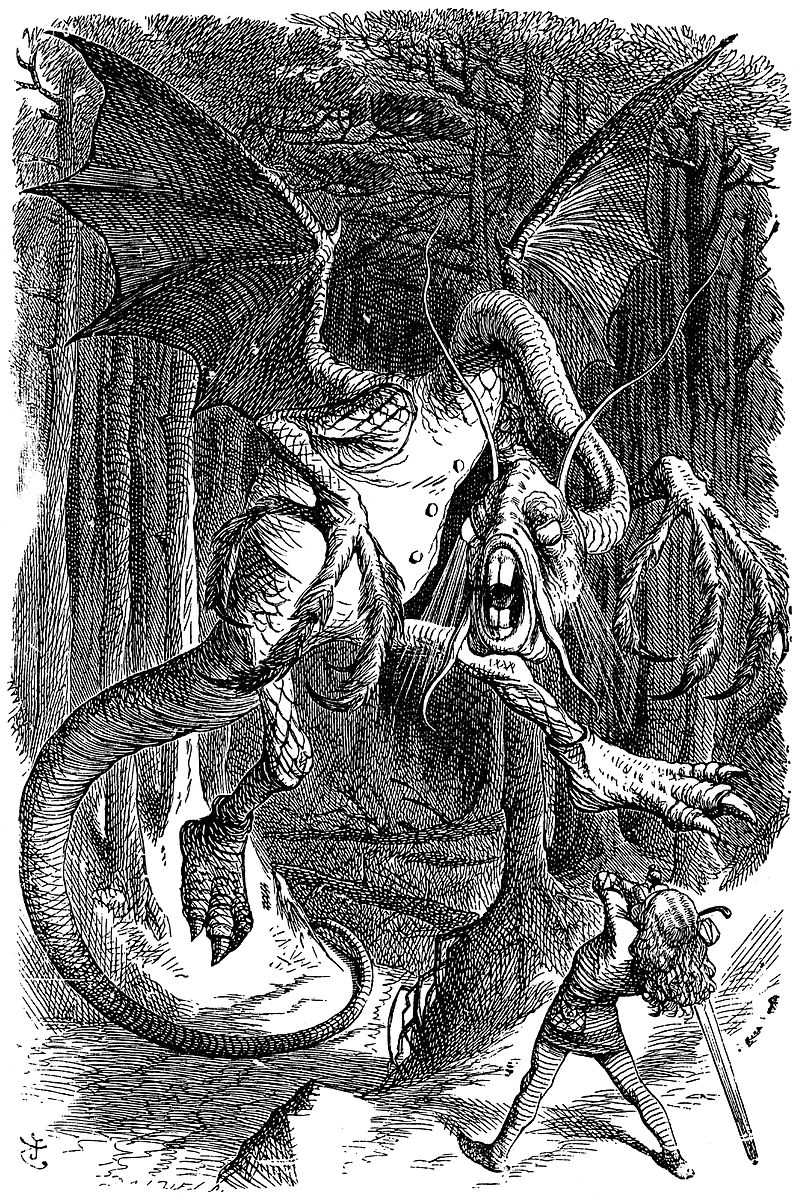
\includegraphics[width=1\textwidth]{img/Jabberwocky.jpg}
% 
% 	%"It seems very pretty," she said when she had finished it, "but it's rather hard to understand!" (You see she didn't like to confess, even to herself, that she couldn't make it out at all.) "Somehow it seems to fill my head with ideas—only I don't exactly know what they are!
% 	"It seems very pretty, [...] somehow it seems to fill my head with ideas—only I don't exactly know what they are!
% 	\source{Through the Looking-Glass, and What Alice Found There}{Lewis Carroll}
% \end{center}
\end{epigraph*}



\chapter{Introduction}

%%%%%%%%%%%%%%%%%%%%%%%%%%%%%%%%%%%%%%%%%%%%%%%%%%%%
\graphicspath{{}{introduction/}{Diagrams/}}

These are exciting times in high-energy physics. The Standard Model (SM), our most powerful and well-tested theory of particles and their interactions, triumphs across the experimental landscape and proves to be much more robust than ever anticipated. Yet, as we will see throughout this thesis, once confronted with some of the simplest questions about the Universe, it provides unsatisfactory answers and, most surprisingly, little theoretical guidance on what may lie beyond. While there is no guarantee that the questions we ask are indeed ``good'' ones, to many, the limitations of the SM attest to the need of a new paradigm in particle physics. Whatever it may be, it makes the series of negative results in particle physics all the more thrilling. Uncertain moments like the one we live are frequent in the history of physics. For many times we saw established theoretical expectations and increasingly fine-tuned models making way for elegant theories like Special Relativity, for new particles such as the neutrino and for new ideas like spontaneous symmetry breaking (SSB).

In practice, of course, such grandiose endeavors are reduced to much less noble but no less important efforts. The frequency of negative results and the need to over-constrain our models make the search for new physics a true exercise in patience. Nevertheless, it is in a persistent and curious spirit that this thesis stands. The common theme of the work developed here is that of \emph{hidden neutrino physics}, both in the sense of rare neutrino processes and of hidden sectors beyond the SM. Hidden, dark or secret are all terms associated with new particles that hide not at high energies with $\mathscr{O}(1)$ couplings, but rather at lower scales with couplings to the SM that are much smaller than one. With the exciting theoretical and experimental prospects in neutrino and dark matter physics, we believe that it is all the more timely to think harder about what neutrinos, hidden particles of their own, may teach us about this type of hidden physics. 

We start this thesis by reminding ourselves of the main features and limitations of the SM in this chapter, and delving into unique aspects of neutrino physics in the next. This way, we hope to set the scene and motivate the direction we pursue in the following chapters. Indeed, the processes of neutrino trident production and neutrino-electron scattering we discuss in Chapter 3 are a testimony of the unique properties of neutrinos and the bright prospects in experimental neutrino physics. As a concrete example, we will see in Chapter 4 how such signatures probe new gauge interactions much weaker than those in the SM ($g \lesssim 10^{-3}$). The fact that neutrinos are the only neutral fermions in the SM also has interesting consequences for mass generation and naturally connects them to neutral hidden sectors. We explore this connection with a specific model at hand in Chapter 5, scrutinizing its phenomenology at short-baselines in Chapter 6. Finally, in Chapter 7 we look towards the far future and highlight the impact of a near-future entry-level neutrino factory in neutrino physics.

\section{The Standard Model}

The Standard Model (SM) of particle physics is a Yang-Mills theory~\cite{Yang:1954ek} of strong, weak and electromagnetic (EM) particle interactions based on an $SU(3) \times SU(2) \times U(1)$ local gauge symmetry. The first remarkable aspect of the theory is in the fact that it relies on the same idea that explains Maxwell's equations, the principle of gauge invariance. In this way, it is hard to pin down the official conception of the SM, although it is widely associated with the appearance of a model first developed by Sheldon L. Glashow~\cite{Glashow:1961tr}, Steven Weinberg~\cite{Weinberg:1967tq} and Abdus Salam~\cite{Salam:1968rm}. Unconcerned with quarks and the strong force, this spontaneously broken $SU(2) \times U(1)$ local gauge symmetry already reflected most of what we know about the electroweak (EW) interactions of leptons nowadays. In fact, the spontaneous broken symmetry that was used already predicted the existence of a charged massive vector boson, the $W^\pm$, a neutral massive vector boson, the $Z$, and of a massless generator of the unbroken $U(1)_{\rm EM}$ group, the photon $\gamma$. Beyond unifying the weak and EM forces, the breaking through the Higgs mechanism~\cite{Higgs:1964ia,Higgs:1964pj} implied that an additional scalar particle, the higgs boson $H$, had to exist. This last prediction was experimentally validated after the discovery of a neutral scalar boson at the LHC in 2012~\cite{Chatrchyan:2012xdj,Aad:2012tfa}, the last SM particle to be experimentally observed.

The strong force had a much richer and more turbulent history. The quark model, developed by Murray Gell-Mann and George Zweig~\cite{Zweig:1981pd,GellMann:1964nj} in 1964, had great success in explaining the growing number of hadronic resonances found by experiments. However, it was not until asymptotic freedom was discovered in non-Abelian gauge theories~\cite{Gross:1973id,Politzer:1973fx} that quantum chromodynamics (QCD) was really born. QCD is an $SU(3)$ local gauge theory describing the interaction of quarks and gluons, and is vastly different from any other theory we will encounter in this thesis. Its uniqueness is best exemplified through color confinement, the property that colored particles must always be present in bound colorless states, called hadrons. For QCD, confinement is guaranteed below the scale $\Lambda_{\rm QCD} \approx 250$ MeV, below which strong processes are non-perturbative. This is to be contrasted with asymptotic freedom, where the strong interactions between quarks and gluons become asymptotically weaker at higher energies. The presence of new degrees of freedom other than quarks and gluons at low energies, namely the hadrons, is a clear evidence of a phase transition and makes QCD a unique topic within the SM. At times we will refer to known results in this theory, but it usually has little bearings on electroweak physics.

\subsection{Fields and symmetries}

We now set out for a more precise definition of the SM field content, discussing some details of local gauge invariance. All fermion fields in the SM are Weyl fields of either definite left-handed (LH) or right-handed (RH) chirality. An equivalent statement is that SM fields are eigenvectors of $\gamma_5$: $\gamma_5 \psi_R = \psi_R$ for RH, and $\gamma_5 \psi_L = - \psi_L$ for LH fields. This is an important feature that allows us to work with 2 component Weyl spinors and makes explicitly manifest the chiral nature of weak interactions. The LH field content and their representation under the different gauge groups is shown in \reftab{tab:SMcharges}. Note that only LH particles transform non-trivially under $SU(2)_L$. Also shown is the Higgs field $H$, a complex scalar field, doublet under $SU(2)$. As we will see in the next section, $H$ is responsible for the breaking of $SU(2)_L \times U(1)_Y \to U(1)_{\rm EM}$.
%
\renewcommand{\arraystretch}{1.4}%
\begin{table}[t]
 \begin{tabular}{lccccccccccc}
 \hline
    & $Q_L^\alpha$& $L^\alpha$ & $\overline{u_R^\alpha\vphantom{d}}$ & $\overline{d_R^\alpha}$ & $\overline{e_R^\alpha\vphantom{d}}$ & &$H$ & & $G$ & $W$ & $B$\\
    \hline
  SU$(3)_c$ & $\bm{3}$ & $\bm{1}$& $\overline{\bm{3}}$ & $\overline{\bm{3}}$ & $\bm{1}$ & & $\bm{1}$ & & $\bm{8}$ & $\bm{1}$ & $\bm{1}$ \\
  SU$(2)_L$& $\bm{2}$ & $\bm{2}$ & $\bm{1}$ & $\bm{1}$& $\bm{1}$& & $\bm{2}$ & & $\bm{1}$ & $\bm{3}$ & $\bm{1}$ \\
  U$(1)_Y$ & $1/3$ & $-1$ & $-4/3$ & $2/3$ & $2$ & & $1$ & & $0$ & $0$ & $1$ \\
  \hline
 \end{tabular}
 \caption[SM field content.]{The representation of the SM left-handed Weyl fields, complex scalar and gauge bosons under each gauge group of the SM. For $U(1)_Y$, the charge is shown instead. All fermions carry a flavour index $\alpha = e, \mu$ or $\tau$.\label{tab:SMcharges}}
\end{table}
\renewcommand{\arraystretch}{1.0}%
%
From the observed EM charges $Q_{\rm EM}$, the $SU(2)_L$ isospin $T_3$, and by virtue of the Gell-Mann-Nishijima formula~\cite{Nakano:1953zz,Gell-Mann:1956iqa}
%
\begin{equation}
 Q_{\rm EM} = T_3 + \frac{Y}{2},
\end{equation}
%
the hypercharge $Y$ of each SM field is fixed. The \emph{local} gauge transformation of the matter fields are given by
\begin{equation}
\psi  \to \exp{i g \theta^a(x) T^a } \psi,
\end{equation}
where $g$ is the gauge coupling constant, $a$ counts the number of generators $T^a$, and $\theta^a(x)$ are arbitrary parameters that depend on space-time coordinates $x^\mu$. To achieve local gauge invariance, we require the following gauge fields associated with each group:
%
\begin{equation}
 SU(3)_C: \{G_1 (x), \cdots, G_8 (x)\}, \quad SU(2)_L:  \{W_1(x), W_2(x), W_3(x)\}, \quad U(1)_Y: B(x),
\end{equation}
%
corresponding to the eight gluons, the $SU(2)$ gauge fields and the hypercharge field. Note that the number of gauge fields matches the number of generators in each group, \eg\ for $SU(N)$ there are $N^2 -1$ generators. For the original $SU(2)\times U(1)$ theory, this implied that in addition to the charged gauge fields, which explained Fermi's theory for beta decays, and the observed massless photon, there must have been an additional neutral gauge field corresponding to some linear combination of $W^3$ of $SU(2)_L$ and $B$ of $U(1)_Y$. This striking prediction was in fact first confirmed by Gargamelle, a bubble chamber experiment, through the observation of accelerator neutrinos scattering into final states with no charged leptons~\cite{Hasert:1973ff}. 

The SM is a non-Abelian theory, since its symmetry group contains direct products of two $SU(N)$, $N > 1$, groups. The generators of a given group equipped with commutators form a Lie Algebra, obeying $[T^a, T^b] = i f^{abc} T_c$, with $f^{abc}$ being the group structure constant. In the special case $f^{abc} = 0$, the generators commute and the group is said to be Abelian, like in the case of $U(1)_Y$. Otherwise, the group is non-Abelian and the theory displays a much richer underlying dynamics. Take an $a$-dimensional Yang-Mills theory and define $\bm{\theta} = T^a \theta^a$ and $U = e^{i g \bm{\theta}}$. We can now perform gauge transformations on the relevant matter fields $\psi$, gauge fields $\bm{A}_\mu = T_a A_\mu(x)^a$ and derivatives of matter fields as follows
%
\begin{equation}
\psi \to U \psi, \quad \bm{A}_\mu \to U \bm{A}_\mu U^{-1} - \frac{i}{g} (\partial_\mu U) U^{-1}, \quad \partial_\mu \psi \to U \partial_\mu \psi +  \psi (\partial_\mu U).
\end{equation}
%
As we can see, the last term is not invariant due to the local character of the gauge transformations. To preserve gauge invariance, a covariant derivative, transforming as $D_\mu \to U D_\mu U^{-1}$, now replaces the ordinary derivative. It is defined as 
\begin{equation}
D_\mu = \partial_\mu + ig \bm{A},\quad \text{such that} \quad D_\mu\psi \to U D_\mu\psi, \,\,\implies\,\,\overline{\psi} i\slashed{D}\psi \to \overline{\psi} i \slashed{D} \psi. 
\end{equation}
%
The invariant term above is the fermion kinetic term. Beyond fermion propagation, it is the main way to describe fermion-gauge interactions in the SM. In particular, the full covariant derivative in the SM is given by
%
\begin{equation}
 D_\mu = \partial_\mu + ig \,W_\mu^a\tau_a + i\frac{Y}{2} g^\prime \,B_\mu + i\frac{g_s}{2} \,G_\mu^b\lambda_b,
\end{equation}
%
where $\tau_a = \sigma_a/2$ are the generators built from Pauli matrices acting on the doublets of $SU(2)_L$, and $\lambda_b$ the generators built from the Gell-Mann matrices acting on the triplet representations of $SU(3)_c$. The factors of $1/2$ come from the canonical  This also fixes the different gauge couplings of the SM. Finally, the gauge invariant kinetic terms for the gauge bosons are 
%
\begin{equation}
\mathscr{L}_{\rm Gauge} = -\frac{1}{4} G^{a}_{\mu\nu} G_a^{\mu\nu} - \frac{1}{4} W^{a}_{\mu\nu} W_a^{\mu\nu} -\frac{1}{4} B_{\mu\nu} B^{\mu\nu},
\end{equation}
%
where $F^a_{\mu \nu} = \partial_\mu F^a_\nu - \partial_\nu F^a_{\mu} - g_F f^{abc} F_{b\,\mu} F_{c\,\nu}$ with $g_F$ the relevant gauge coupling. The kinetic term in Abelian theories concern only the propagation of gauge bosons, however, for non-Abelian groups the term proportional to $g_F$ in $F^a_{\mu \nu}$ introduces interactions among the gauge bosons proportional to $g$ and $g^2$. Therefore, a non-Abelian theory is already an interacting theory without the addition of any matter fields.


\subsection{Spontaneous symmetry breaking}

So far we have only discussed the gauge and fermionic content of the SM. The scalar sector is, in fact, quite special. The only scalar particle, the higgs boson, is responsible for spontaneously breaking $SU(2)_L\times U(1)_Y$ to $U(1)_{\rm EM}$ after it acquires a non-zero vacuum expectation value (vev). This introduces a mass scale in the theory which, apart from dimensionless couplings, sets the scale of EW physics. Note that because it is a scalar particle, a non-zero vev does not violate the symmetries of space-time, namely Lorentz invariance. The higgs is a complex scalar field and a doublet under  $SU(2)_L$, and so we can write
%
\begin{equation}
  H =  \frac{1}{\sqrt{2}} \left( \begin{matrix}  G_1^+ + i G_2^+ \\  h^0 + i G_3^0 \end{matrix} \right) =  \frac{e^{i G_a \tau^a}}{\sqrt{2}} \left( \begin{matrix} 0 \\  h \end{matrix} \right).
\end{equation}
%
The relevant Lagrangian in the SM reads
%
\begin{equation}
\mathscr{L}_{\rm higgs} \supset \left( D^\mu H \right)^\dagger \left( D_\mu H \right) - V(H), \qquad V(H) = \mu^2 H^\dagger H + \lambda \left( H^\dagger H \right)^2.	
\end{equation}
%
where $\mu^2$ has mass dimension 2, being the only dimensionful parameter in the SM. If $\mu^2 < 0$, minimizing the potential $V(H)$ requires $\bra{0} H \ket{0} = \left( 0, \,\, v/\sqrt{2} \right)^T$, where $v^2 = - \mu^2 /\lambda$ is the vev chosen to lie in the real and neutral direction. We now can then expand around the true vacuum of the theory by redefining the fields $G_a \to G_a/v$ and $h \to h + v$. At this point, a rewriting of the potential reveals the mass and interactions of every component of the scalar doublet. Note, however, that it contains no mass terms for $G_1$, $G_2$ and $G_3$. These are the Goldstone bosons of the theory, and although they are massless, they do possess interactions with the scalar and gauge boson fields. One way to understand their role is to perform an $SU(2)_L \times U(1)_Y$ gauge transformation in our Lagrangian such that the resulting higgs doublet reads
%
\begin{equation}
H \to e^{- i G_a \tau^a/v} H =  \frac{1}{\sqrt{2}}\left( \begin{matrix}  0 \\ h + v \end{matrix} \right).
\end{equation}
%
This transformation must also be applied to the gauge fields, fixing the gauge. This particular choice is rather convenient and is known as the unitary gauge. We then find
%
\begin{align}
 \mathscr{L}_{\rm higgs} &\supset - \frac{1}{2} m_h^2 h^2 - \lambda v h^3 - \frac{\lambda}{4} h^4  \nonumber\\ &\qquad\qquad +  M_\textsc{w}^2 W_\mu^\dagger W^\mu \left[ 1 + \frac{2 h}{v} + \frac{h^2}{v^2}\right] + \frac{M_\textsc{z}^2}{2} Z_\mu Z^\mu \left[ 1 + \frac{2 h}{v} + \frac{h^2}{v^2}\right],
\end{align}
%
where $m_h = \sqrt{2\lambda}\, v = 125.18 \pm 0.16$ GeV~\cite{PDG}. Most importantly, after SSB, the higgs kinetic term has given us three massive and one massless vector bosons, defined as
\begin{equation}
 W^\pm_\mu = \frac{1}{\sqrt{2}} \left(W^1_{\mu} \mp i W^2_{\mu} \right), \quad Z_\mu = c_\textsc{w} W^3_\mu - s_\textsc{w} B_\mu, \quad A_\mu = c_\textsc{w} B_\mu - s_\textsc{w} W^3_\mu.
\end{equation}
% 
where $s_\textsc{w}$ ($c_\textsc{w}$) is the sine (cosine) of the weak angle, defined by $c_\textsc{w} = g/\sqrt{g^2 + g^{\prime\,2}}$. These fields correspond to the mediators of the weak charged-current interactions ($M_\textsc{W} = g v/2 = 80.387\pm 0.016$ GeV~\cite{PDG}), weak neutral-current ($M_\textsc{z} = M_\textsc{w}/c_\textsc{w} = 91.1876\pm0.0021$ GeV~\cite{ALEPH:2005ab}) neutral boson and the massless photon $A_\mu$, mediator of the unbroken EM interactions. They interact with the higgs boson via the triple and quadruple vertex terms above. The interactions with matter are obtained from the fermion kinetic terms, where the charged, neutral and electromagnetic currents are defined and written as
%
\begin{equation*}
\mathscr{L}_{\rm NC} = e \,{J}_\mu^\gamma A^\mu + \frac{g}{c_\textsc{w}}\, {J}_\mu^Z Z^\mu, \quad {J}_\mu^\gamma =  \overline{\psi} Q_{\rm EM} \gamma_\mu \psi, \quad %
{J}_\mu^Z = \overline{\psi} \gamma_\mu \left[ \left( \frac{T_3}{2} - Q_{\rm EM} s_\textsc{w}^2 \right) - \frac{T_3}{2} \gamma^5\right] \psi,
\end{equation*}
\begin{equation}
\mathscr{L}_{\rm CC} = \frac{g}{\sqrt{2}}  \, \left( {J}_\mu^+ W^{\mu \,+} + {J}_\mu^- W^{\mu \,-} \right), \quad
%
{J}_\mu^+ = \frac{1}{2} \overline{\psi}_u \gamma_\mu \left( 1 - \gamma^5\right) \psi_d + {\rm h.c.},
\end{equation}
%
where $\psi \in \{ \nu_L, e_L, u_L, d_L, e_R, u_R, d_R \}$, and $\psi_{u,\,d}$ denoting fermions with $T_3 = \pm 1/2$. From the weak currents we note two important aspects: \emph{i)} weak interactions indeed violate parity and possess a $V-A$ structure, \emph{ii)} charged-current interactions are purely LH as they should be since no RH fields are charged under $SU(2)_L$. After SSB, only the EM current is conserved $\partial^\mu J_\mu^\gamma = 0$. 

In the discussion above, we fixed the gauge of the SM to simplify the EW Lagrangian. This is not necessary and, in fact, another possibility is to keep all terms involving the Goldstone fields $G_a$ and eliminate off-diagonal kinetic terms of the type $Z_\mu\partial^\mu G_3$ by introducing the following gauge breaking Lagrangian to the SM
\begin{equation}
 \mathscr{L}_{\rm R_\xi} = -\frac{\left(\partial_\mu A^\mu\right)^2}{2 \xi_\gamma} - \frac{\left(\partial_\mu Z^\mu + \xi_Z M_Z G_3^0 \right)^2}{2 \xi_Z} - \frac{\left|\partial_\mu W^{\mu\,-} + i \xi_W M_W G^- \right|^2}{2 \xi_W}.
\end{equation}
This is known as the $R_\xi$ gauge, where the explicit dependence on the gauge breaking parameters $\xi$ serves as a useful diagnostic of gauge invariance in physical observables. The Lorentz gauge is recovered for $\xi = 0$ and the Feynman-'t Hooft gauge with $\xi = 1$. The additional advantage of using this method is that it allows us to trace the Goldstone degrees of freedom. The pseudoscalar fields $G^\pm$ and $G_3$ end up behaving very similarly to the $W^\pm$ and $Z$ gauge bosons. In fact, at high-energies it can be shown that the Goldstone bosons are equivalent to the longitudinal polarization states of their respective gauge bosons~~\cite{Cornwall:1974km,LlewellynSmith:1973yud}. This is known as the Goldstone boson equivalence theorem, and it turns out to be very important to understand processes like $W_L \, W_L$ and $Z_L \,Z_L$ scattering. At very high-energies and without the Higgs boson, such processes grow indefinitely ($\sigma \propto s$), spoiling the unitarity of the $S$-matrix. The fact that this problem was solved by including contributions from $h$ exchange provided a no-lose theorem for the LHC: either the higgs boson would be discovered, or new physics must appear to unitarize these processes. 

\subsection{Fermion masses}

The EW sector is also responsible for the generation of fermion masses in the SM. As noted before, all LH fermions in the SM are $SU(2)_L$ doublets, just like the higgs. This allows us to construct the so-called Yukawa terms,
%
\begin{equation}
 \mathscr{L}_{\rm Yukawa} =  y_e \left(\overline{L}_\alpha H\right) e_R +  y_u \left(\overline{Q}_L \tilde{H} \right) u_R + y_d \left(\overline{Q}_L H \right) d_R  + \,\, {\rm h.c.},
\end{equation}
%
where we defined the charge-parity (CP) conjugated higgs field $\tilde{H} = i \sigma_2 H^* = ( h + v + i G_3, \,\, G_1 - i G_2  )^T$. After SSB, these interaction terms endow charged-leptons and quarks with a dirac mass term of the form
\begin{equation}
 m_\psi \overline{\psi} \psi = m_\psi \left( \overline{\psi}_L \psi_R +\overline{\psi}_R \psi_L \right),\quad {\rm with} \quad m_\psi = \frac{y_\psi \, v}{2},
\end{equation}
where $\psi_{L,\,R} = P_{L,\, R} \, \psi = (1 \mp \gamma_5)\, \psi/2 $ are the chiral projections of the fermion field $\psi$. To include all three families of fermions we promote $y_\psi \to \bm{y}_\psi$, a $3\times3$ matrix. 

In the quark sector, the Yukawa matrix is off-diagonal and the different generations mix. The physical quark masses are found after rotating the up and down quarks, left and right, as $u_{L,\, R}^\alpha = \left(V_{L,\,R}^{u\,*} \right)_{\alpha i} u^i_{L,\, R}$ and $d_{L,\, R}^\alpha = \left(V_{L,\,R}^{d\,*} \right)_{\alpha i} d^i_{L,\, R}$. The diagonal mass matrix is then $\bm{m}^{u,\,d} = \bm{V}_L^{u,\,d} \bm{y}_{u,\,d} \bm{V}_R^{u,\, d\,\dagger} v/\sqrt{2}$. Note that after this procedure we cannot help but introduce mixing in the charged current. This defines the Cabbibo-Kobayashi-Maskawa (CKM) matrix~\cite{Cabibbo:1963yz,Kobayashi:1973fv}, $\bm{V}_{\rm CKM} = \bm{V}_L^u \bm{V}_L^{d\, \dagger}$. The CKM matrix is nearly diagonal, so the mixing between quark flavour and mass eigenstates is small. From the unitarity of the rotation matrices, neutral currents remain invariant 
\begin{equation}
\sum_{\alpha,\, \beta} \overline{\psi}_L^\alpha \,\Gamma^\mu \, \psi_L^\beta = \sum_{i,\,j} \overline{\psi}_L^i \, \left( \sum_{\alpha,\, \beta} (V_L)_{\alpha i} (V_L^*)_{\beta j}\right) \,\Gamma^\mu\, \psi_L^j =  \sum_{i,\,j} \overline{\psi}_L^i \, \,\Gamma^\mu\, \psi_L^j,
\end{equation}
%
where $\Gamma^\mu$ are the neutral-current couplings and gamma matrices.  Crucially, the latter have no flavour dependence and so the SM forbids flavour changing neutral currents (FCNC). This mechanism was first proposed by Glashow, Illiopoulous and Maiani to explain why decays of the type $K^0 \to \mu \mu$ were unobserved. Famously referred to as the GIM mechanism, this relies on the flavour universal nature of SM neutral currents and on the unitarity of the CKM. As we will see, this mechanism also plays an important role in the neutrino sector and in many extensions of the SM.

Summarizing, we saw how a single parameter with massive dimensions in the scalar potential of the SM leads to SSB. This is then ``propagated'' to the rest of the SM through the higgs kinetic terms and Yukawa couplings. At this point it is possible to appreciate two problems with the SM mass generation mechanism. Firstly, it implies that all Yukawa couplings are just parameters to be inferred from the measured masses of particles. That is, the SM makes no statements and provides no explanations as to why the Yukawas that we observe in nature are what they are. This is known as the flavour puzzle: what explains the different observed values of the fermion masses? This problem is aggravated when we consider the lepton sector, where neutrino masses and mixing are drastically different from the quark sector. The second problem concerns the neutrino sector, and is perhaps the biggest motivation behing studying neutrino physics. The SM predicts exaclty massless neutrinos in the absence of $\nu_R$ fields. Although  

Before moving on to more speculative topics, a few comments are in order. EW SSB seems to be, as far as we know, a real phenomenon. It explains why the symmetries of the SM were so well hidden the first place: true symmetries of Nature seem to not be shared by the vacuum. While the evidence for EW SSB comes mainly from studying fundamental particles, its consequences do not concern only particle physics. EW physics helps us understand the past and future of our own Universe. In the early Universe, at hight temperatures, it is expected that the EW symmetry is restored~\cite{Kirzhnits:1972ut,Dolan:1973qd,Weinberg:1974hy}. If this is the case, the EW phase transition provides a unique test of the higgs mechanism and points to a completely different Universe from our own, where finite temperature effects and non-perturbative physics play a major role. In addition, we have no reason to expect the vacuum structure of the Universe to be as simple as in the discussion above. After all, the stability of our own vacuum is not even guaranteed within the SM~\cite{Cabibbo:1979ay,Degrassi:2012ry}. Radiative corrections to the higgs self-coupling $\lambda$ alter the shape of the scalar potential and imply we may live in a local, rather than global, minimum of the potential. For these reasons, studying the higgs sector, confirming that it generates all fermion masses in the SM and why it seemingly fails to do so in the case of the neutrino are all important questions worth pursuing.

\begin{figure}
 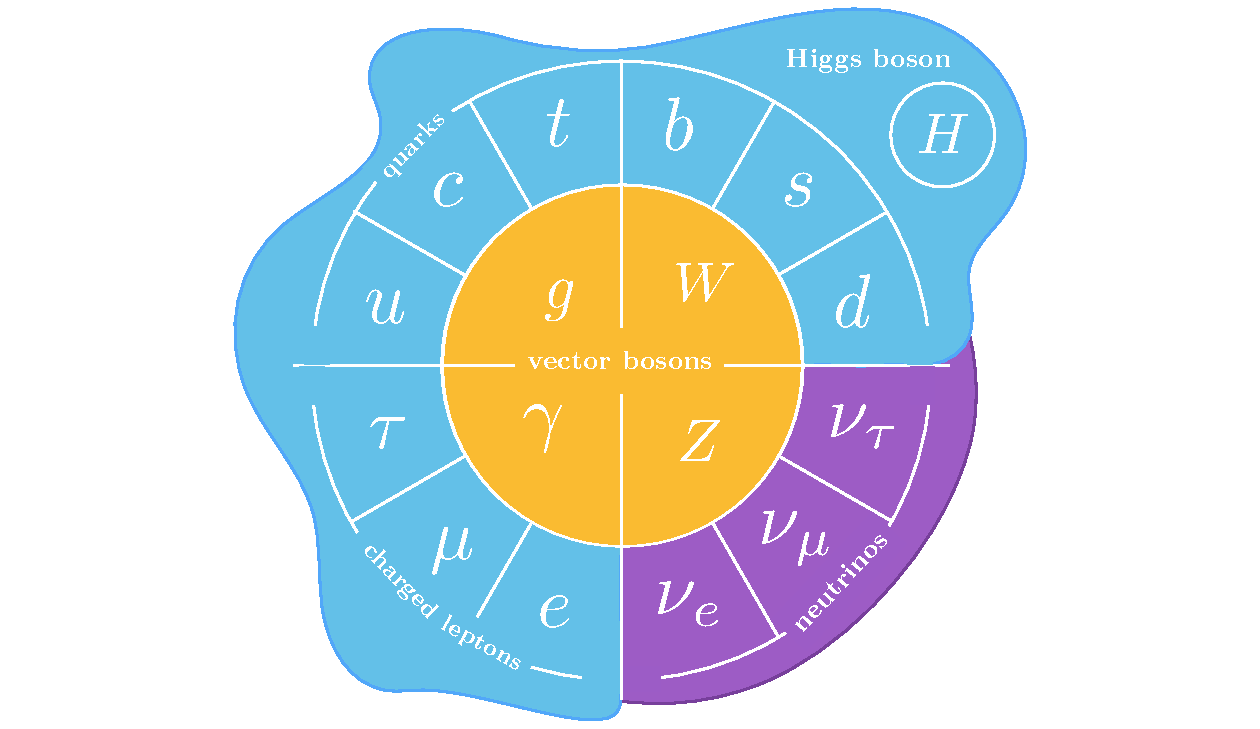
\includegraphics[width=0.96\textwidth]{SM_zoo.pdf}
 \caption{Artistic rendering of the particles in the Standard Model. \label{fig:SM_diagram}}
\end{figure}



%%%%%%%%%%%%%%%%%%%%%%%%%%%%%%%%%%%%%%%%%%%%%%%%%%%%%%%%%%%%%%%%%%%%%%%%%%%%%%%%
%
% BSM!!!!!!
%
%%%%%%%%%%%%%%%%%%%%%%%%%%%%%%%%%%%%%%%%%%%%%%%%%%%%%%%%%%%%%%%%%%%%%%%%%%%%%%%

\section{Evidence for Beyond the Standard Model physics}

The most important building aspects and building blocks of the SM have been laid out above. Now, a different question will concern us: is this theory sufficient to explain fundamental particles and their interactions? We have already stumbled upon a few problems of the SM, but even before that one must already suspect that the SM is not a final theory. It does not explain gravity. This tells us that the SM should be treated as an effective theory valid up until the Planck mass $M_{\rm Pl} = \left(\hbar c/ 2 G_{\rm Newton}\right)^{1/2} \approx 10^{19}$ GeV, where the effects of gravity are expected to be large~\footnote{This is a naive expectation based on the observation that the Schwarzschild radius $\ell_s = 2 G_{\rm Newton} m/c^2$ and the Compton wavelength $\ell_c = h /mc$ of a particle become comparable at $m \approx M_{\rm Pl}$.}. This very own fact already brings us to one of the most controversial evidences for beyond the Standard Model (BSM) physics.

\paragraph{The hierarchy problem} The lack of evidence for new physics at the LHC can be argued to be more than just unfortunate. If no new physics is indeed present between the EW and the Planck scale, then the cut-off of the SM, beyond which the effective field theory is no longer valid, is $\Lambda = M_{\rm Pl}$. This implies that unless symmetries are at play, terms of dimensions $d$ are suppressed or are of the order of $\Lambda^{4-d}$. However, in the SM $m_h^2 \ll \Lambda$, suggesting a fine-tuning of many orders of magnitude. Quantum corrections to the higgs mass, $m_h^2 = m^2_{\rm bare} + \delta m_h^2$, are dominated by the top quark and go as $\delta m_h^2 = y_t^2 \Lambda^2 / 8 \pi^2$. This quadratically divergent result implies that to obtain the observed light higgs mass, whatever new physics that may appear at the scale $\Lambda$ (possibly even below $M_{\rm Pl}$) must cancel the fermion loops to order $m_h^2/ \Lambda^2$. In other words, the matching condition for the renormalization of $m_h^2$ parameter becomes fine-tuned to order $m_h^2/ \Lambda^2$ in the presence of such cut-off. Supersymmetric theories are notorious candidates that solve this problem, but so far we are yet to find any evidence for them. One may argue that indeed there exists a ``desert'' between the EW and the Planck scale, and that some miraculous mechanism is at play in quantum gravity that may solve the fine-tuning problem. In that case, a solution to all following items in this list must be found there, or somewhere outside the realm of particle physics.

\paragraph{The strong-CP problem} The QCD Lagrangian admits the following field-strength contraction term
%
\begin{equation}
 \mathscr{L} \supset \frac{\theta \alpha_s^2}{8\pi} G_{\mu\nu}^a \tilde{G}_a^{\mu\nu},\quad {\rm where }  \quad \tilde{G}^a_{\mu\nu} = \frac{\epsilon_{\mu\nu\rho\sigma}}{2} {G}^{a\, \rho\sigma}.
\end{equation} 
This can be shown to be a surface term (a total divergence in the action) and can be neglected in perturbative calculations. Nevertheless, this term induces CP violation in the strong sector via non-perturbative effects, leading to a large electric dipole moment for free neutrons~\cite{Crewther:1979pi}, which is orders of magnitude above the experimental upper limits~\cite{Afach:2015sja}. The most popular scenario to explain the smallness of $\theta$ is the Peccei-Quinn symmetry~\cite{Peccei:1977ur}, a global chiral $U(1)$. The breaking of this symmetry leads to the prediction of a Goldstone boson, the axion.

\paragraph{Matter-antimatter asymmetry} The observed baryon asymmetry of the Universe contradicts the standard Cosmology, which predicts that matter and anti-matter were created in equal amounts in the Big Bang. The SM does not provide enough source of CP violation to explain this phenomenon. Popular scenarios to explain this are EW baryogenesis and Leptogenesis, where the latter relies on the CP violation from a heavy neutrino sector and its translation into a baryon asymmetry through Spharelon processes.

\paragraph{Dark matter} Measurements of the redshift of galaxy clusters in the 1930's~\cite{Zwicky:1933gu} and galaxy rotation curves in the 70's~\cite{Rubin:1970zza}, are among the pioneering work that showed that the gravitational potential in such astrophysical scales is much deeper than the one extrapolated from luminous matter. Already at the time, astronomers would refer to the source of this additional gravitational influence as Dark Matter (DM). As Astrophysics and Cosmology evolved, concrete evidence for DM continued to build up. Evidence for DM is now present at a variety of scales, from the precise measurements of the cosmic microwave background (CMB)~\cite{Akrami:2018vks}, the matter distribution in galaxy cluster mergers~\cite{Clowe:2006eq}, and the observed large scale structure of the Universe~\cite{Blumenthal:1984bp}. In fact, from CMB power spectrum we can infer the DM density today as~\cite{Akrami:2018vks}
\begin{equation}
 \Omega_{\rm DM} h^2 = 0.1200\pm0.0012
\end{equation}
with $\Omega_{\rm DM} = \rho_{\rm DM}/\rho_c$ the energy density of DM in units of the critical density $\rho_c \approx 10^{-26}$ kg/m$^3$, and $h = H_0/(100$ km s$^{-1}$/Mpc$^{-1}) = 0.674\pm0.005$ the scaled Hubble expansion rate. This is roughly five times larger than the density of baryons, understood as all other non-relativistic matter. The latter is also measured through the relative abundances of light elements during Big Bang Nucleosynthesis (BBN)~\cite{Cooke:2013cba}, where DM plays no role and providing further evidence for non-baryonic DM.

The nature of DM is not yet understood and many possibilities are under discussion. Modified gravity models explain local astrophysical observations, but struggle to explain all CMB datasets and X-ray observations of mergers of galaxy clusters~\cite{Famaey:2011kh}. Primordial black holes~\cite{Barack:2018yly} have also been put forward as DM candidates and have triggered great interest due to their connection to the detection of gravitational waves. However, the most popular hypothesis at this point remains that DM is made of new particles. This new state better be neutral, to have evaded our detection, and sufficiently long-lived, so that it may linger until today after its production in the early Universe. The fluid of such particles would have to display negligible pressure and viscosity, and to have been created cold so as to help form clumpy structures in the Universe with its gravitational influence. This points us to a particle that is massive, collisionless and, yet, very abundant today. Most notably, DM models have often focused on the possibility of a weakly-interacting massive particle (WIMP). In this paradigm, DM particles, say $\chi$, are produced in the early Universe through its weak interactions with the SM plasma. At later times, approximately at temperatures of the order of the DM mass $m_{\chi}$, DM production stops and annihilation into SM particles dominates. As the Universe cools and expands, the DM gas is diluted and annihilation is no longer effective, \emph{freezing-out} the DM population at around $T \approx m_{\chi}/20$. In particular, the relic density obtained in this mechanism is of the order $\Omega_\chi H_0^2 \approx 0.1 \,{\rm pb}/ \sigma$, where $\sigma$ stands for the thermally averaged cross section of $\chi$ annihilation into SM particles. The fact that $\sigma\approx 1$ pb allows to reproduce the current DM density and is of the order of typical weak cross sections (as in mediated by weak bosons) is known as the WIMP-miracle. WIMP DM is a collisionless and thermal candidate, although DM candidates that are non-thermal, or collisionless, or both exist.

\paragraph{Neutrino masses} One of the most important evidences for BSM physics is the fact that neutrinos have mass. This comes from the plethora of experimental evidence for neutrino oscillations, which we explore in the next chapter. Put simply, neutrino oscillation data requires at least 2 non-zero and non-degenerate massive neutrinos. Although one might argue that this is solved by the mere addition of at least 2 RH neutrino states to the SM which are complete singlets of the symmetry, this simple extension still requires further study and experimental confirmation. In addition, such states would be the only SM particle to admit a Majorana mass term of the type $M \,\overline{\nu^c}_R \nu_R$, and unless new symmetries are introduced, there is no reason to expect that $M$ is exactly zero. Therefore, it is customary to think that neutrino masses are the first indications of physics beyond the SM observed in controlled laboratory conditions.   

\section{Extending the Standard Model}

In extending the SM one may take several approaches. We can be guided by experimental results and tensions, by increased symmetries and elegance in our theories, or by complete agnosticism. While we lack a single compelling evidence for the direct detection of a new particle, we can interpret many of the problems outlined above as evidence for new states. The existence of DM and neutrino masses, in particular, suggests (but does not require) that these new states may be a new sector of electromagnetically neutral particles. Here, the SM provides no guidance for their masses or symmetries, and so a mixture of all three approaches outlined before is common in the literature. This thesis is no exception.

Dark sectors are a typical prediction of theories with 


Our BSM extensions all involve light and hidden new states, which have evaded detection to the smallness of their couplings to the SM. This point of view is compelling from a DM and neutrino perspective.

only neutral particle in the SM , in the spotlight 

In this sense, our job is to search ``under the lightpost'', using current and future experiments to look for new physics in a opportunistic way. Not only is this a cheap and viable exercise, it would offers an explanation as to why the SM performs so well as a theory and against most experimental tests. A modular view of the Universe, with the visible SM sector and potential dark sectors barely influencing each other wou

Given the hints that dark sectors beyond the SM may exist, we would like to investigate all the possible ways the particles in this sector may interact with the SM. One way to tackle this question is to build effective field theories, where one studies all operators which are allowed by the content and symmetries of the SM. The idea is to construct a series of $d>4$ operators in $1/\Lambda^{d-4}$, where $\Lambda$ is the scale of the new physics. This approach thrives on its generality, but can become complicated very quickly with growing $d$. Most importantly, the scale $\Lambda$ is assumed to be large, so that all new degrees of freedom have been integrated out of the theory. This is suitable for extensions involving particles which are very heavy, but the series is no longer well defined for new physics that is light and kinematically accessible at our experiments. In this case, the kinematics of the new particles play a role, forcing us to write down the field content and symmetry group of the new physics. This is the approach we will follow in this thesis.

\subsection{Portals to hidden sectors}

We would like our SM extensions to follow specific guiding principles and organize them in a meaningful way. One way to do so is to study all the low dimension neutral operators that the SM has to offer. In contrast to effective field theories, we want renormalizable operators with $d<4$ which are also gauge invariant. As it turns only a few such operators exist, which we usually refer to as \emph{portals}. We dedicate this section to presenting these.

\paragraph{Neutrino portal} Arguably the most motivated portal, this $d=5/2$ operator can be written as
\begin{equation}
\left( \overline{L}^\alpha_a \cdot \tilde{H}\right), %= \left( \left(\nu^\alpha_L\right)_a \,\, \left(e_L\right)_a \right)
\end{equation}
%
where we made the spinor index $a$ explicit. Any fermion field which couples to this operator acquires couplings to SM neutrinos. This typically induces off-diagonal mass terms in the Lagrangian, leading to mixing between the new species and all massive neutrinos in the broken phase of the SM. The new particle is then commonly referred to as \emph{heavy neutral lepton} or right-handed neutrino, though its chirality is a matter of convention.

\paragraph{Vector portal} Any new vector particle $X^\mu$ may couple to the $d=2$ field strength of the SM hypercharge
\begin{equation}
B_{\mu\nu},
\end{equation}
through its own field strength tensor $X^{\mu\nu}$. The resulting term, $B_{\mu\nu} X^{\mu\nu}$, is a off-diagonal kinetic term for the massive bosons and is sometimes called the \emph{kinetic mixing} operator. To work in a basis of physical states with diagonal kinetic terms, where the propagators are in their standard form, one usually performs a field redefinition. If much lighter than the EW scale, the new vector particle couples primarily to the EM current, hence the name dark photon. If heavy, it can also couple to the NC and is therefore referred to as a dark $Z$. Models with the term 
%
\begin{equation}
 Z_\mu X^\mu 
\end{equation}
%
also come up in the literature, where it is said that \emph{mass-mixing} between the new vector particle and the SM $Z$ exists. This term is not gauge invariant, but may arise in the broken phase of BSM theories with additional doublet scalars, like in two-higgs-doublet models (2HDM). In this case, several charged degrees of freedom typically appear and experimental constraints tend to be more severe.

\paragraph{Higgs portal} New scalar particles can couple to the $d=2$ bilinear 
%
\begin{equation}
 H^\dagger H,
\end{equation}
%
the only renormalizable portal with no free Lorentz or spinor indices. In this case there are two possibilities for a scalar to couple to the SM, depending on its charges. We can write  $H^\dagger H \, S^\dagger S$ for a charged, or $H^\dagger H\, S $ for a singlet complex scalar. The latter term is the only super-renormalizable operator connecting the SM fields to new physics which is allowed. Beyond important consequences for EW SSB, these operators typically inherit the higgs couplings to matter fields, and may be hard to search for due to the smallness of the SM Yukawa couplings. A very simple BSM model with such portal arises in scalar singlet $S$ extensions, where one generates the term $H^\dagger H \, S^\dagger S$~\cite{Silveira:1985rk}. Remarkably, this extension can also have consequences to the "little hierarchy" problem, as the new scalar also contributes to the Higgs self-energy~\cite{Craig:2013xia}.


\paragraph{Fermionic currents}

A whole set of neutral operators in the SM come from the fermionic currents
\begin{equation}
 J^\mu \equiv \overline{\Psi} \gamma^\mu \Psi,
\end{equation}
where $\Psi \in \{Q_L, L, u_R, d_R, \ell_R\}$. This provides SM currents which can be associated with new conserved charges, which in turn may be promoted to a local or global gauge symmetry. The first condition is that it be locally conserved $\partial_\mu J^\mu = 0$. 

\paragraph{Pseudo-scalar} Axions~\cite{Weinberg:1977ma}.






\chapter{Aspects of neutrino physics}
\graphicspath{{}{theory/}{Diagrams/}}

This chapter is dedicated to studying some important and more technical aspects of neutrino physics for the rest of the thesis. We start by reviewing some of the most popular models to explain non-zero neutrino masses beyond the SM. This will be useful to introduce neutrino masses and mixing, with which we can comment on neutrino oscillations in vacuum and in matter. We then move on to discuss the usual approach to studying neutrinos in the laboratory, focusing on accelerator experiments. We will find that it is hard to ignore the strong force in many of the most important neutrino cross sections.

%%%%%%%%%%%%%%%%%%%%%%%%%%%%%%%%%%%%%%%%%%%%%%%%%%%%%%%%%%%%%%%%
%
% MASS MODELS
%
%%%%%%%%%%%%%%%%%%%%%%%%%%%%%%%%%%%%%%%%%%%%%%%%%%%%%%%%%%%%%%%%%%

\section{Mass Mechanisms}

Understanding the theoretical origins of neutrino mass and mixing is a worthwhile but ambitious task. The possibilities are endless and the high-scale dynamics, typical of many neutrino mass models, is hard to test in the laboratory. Presently, it is fair to say there are more neutrino mass models than ways to test them. Nonetheless, many of these models possess similar features and just a couple of low energy observables is sufficient to probe a large class of models. These models may rely on the seesaw mechanism, on radiative effects or in extended scalar sectors. On top of that, new symmetries and fundamental forces may also be at play, making the theories more predictive. We will now explore a small fraction of this model space.

We have already alluded to the first possibility to introduce light neutrino masses in the SM. All that is needed are at least two RH neutrino fields, singlets under all SM symmetries. We shall refer to them as $N^\alpha$, where $\alpha$ is their generation index. This may be chosen to be $\alpha = e, \mu, \tau$ or any combination of two of these. The full new neutrino mass Lagrangian then becomes
%
\begin{equation}\label{eq:typeILagrangian}
 \mathscr{L}_{\nu-{\rm mass}} = \overline{N}^\alpha i\slashed{\partial} N_\alpha - y^\nu_{\alpha\beta} \left( \overline{L}^\alpha \widetilde{H} \right) N^\beta - \left(y^\nu_{\alpha\beta}\right)^* \overline{N^\beta} \left( \widetilde{H}^T  L^\alpha\right)  - M_{\alpha \beta} \overline{N^c}^\alpha N^\beta,
\end{equation}
%
where $N^c = C \overline{N}^T$ with $C$ the charge conjugation matrix ($C = i \gamma^2 \gamma^0$ in the Dirac and Weyl representation). The middle terms endow neutrinos with Dirac masses, but the last one is a new ingredient. This is the Majorana mass matrix for the new RH neutrinos, and it is allowed by the symmetries of the model. It does, however, violate any $U(1)$ symmetry associated with the fields $N$, as
%
\begin{equation}
 N \to e^{i\theta} N \,\implies\, \overline{N^c} N \to e^{2i\theta}\overline{N^c} N.
\end{equation}
%
So if $N$ are assigned lepton number, then the accidental global symmetries of the SM $B-L$ and $L$ are violated by the Majorana mass term. If we insist and set $L(N)=0$, then the Dirac mass term will, instead, explicitly break these global symmetries. This interesting observation, together with the fact that gauging $B-L$ leads to an anomaly-free theory with three RH neutrinos, has led proposals of Dirac neutrino mass models with gauged and unbroken $B-L$~\cite{Heeck:2014zfa}. On top of that, the scale of the entries in $\textbf{M}$ is not set by the Higgs vev and, therefore, may be wildly different from the EW scale. We may argue that it has to be small, since in the limit that all $M_{\alpha\beta}\to0$, the SM symmetry is enhanced and the theory is said to be technically natural in the t'Hooft sense. Regardless of our argument to prevent this term, one thing is clear, a purely Dirac neutrino mass model has to deal with the fact that the neutrino Yukawas are extremely small $y^\nu/y^t \approx 10^{-12}$. If the arbitrariness of Yukawa couplings in the SM already made us uncomfortable, this SM extension dramatically worsens the picture. Of course, we may be tempted to ignore the flavour puzzle and just stop here. This solution, however, as underwhelming as it is, is not unique. Many other models for neutrino masses exist and, while we cannot rule all of them out, it is worthwhile to study the alternatives.

In the same way that the $N$ particles admitted a Majorana mass term, we may wonder if the SM may also provide a similar term for the LH states. Clearly $SU(2) \times U(1)$ invariance forbids any renormalizable operator that would give rise to this operator before SSB, but at $d=5$, we can write the so-called Weinberg operator
%
\begin{equation}\label{eq:weinberg}
 \mathscr{L}_{d=5} = \frac{c_{\alpha\beta}}{\Lambda} \left( \overline{L^c} \widetilde{H}^* \right) \left( \widetilde{H}^\dagger L  \right) \to  \frac{c_{\alpha\beta}}{\Lambda} \frac{v^2}{2} \overline{\nu_L^c}^\alpha \nu_L^\beta
\end{equation}
%
where we go from the unbroken to the broken phase. This operator is, in fact, the only $d=5$ operators allowed in the SM effective field theory (SMEFT). The fact that the lowest dimension non-renormalizable operator in the SMEFT gives neutrino masses is, yet again, another indication that neutrino masses point towards BSM physics. Unfortunately, assuming the coefficients to be $\mathcal{O}(1)$ and saturating the upper bound on the sum of neutrino masses $m_\nu \lesssim 0.1 $ eV, we are led to conclude that $\Lambda \approx 10^{14}$ GeV, eerily close to the Planck scale. There is, however, no reason to expect the couplings of the theory to be large and for the mass mechanism to be simple. Technical naturalness, for instance, is commonly invoked to claim that the mass mechanism may reside at low scales, where we trade unreachable energies for tiny couplings. We will shortly see all tree-level UV-completions to the Weinberg operator. Of course, neutrino masses need not be tree-level effects, and loop-induced mechanisms for generating Dirac or Majorana neutrino masses are also important. In this case, the smallness of neutrino masses is explained through loop suppression factors. We come back to these issues in \refsec{sec:seesaws}.


The mass term induced by \refeq{eq:weinberg} turn out to be of the Majorana kind. Testing this hypothesis is extremely difficult because of the smallness of $m_\nu$. Any process containing lepton number violation (LNV), the hallmark of Majorana neutrinos, will be suppressed by $m_\nu^2/E^2$, where $E$ is the typical energy involved. Another way to understand this is that any process where the operator above is important must be sensitive to the effects of neutrino mass, which we have yet to measure. Curiously, this holds also for neutrino oscillations. In that case, one might also worry about additional phases that appear in the Majorana case, but these can be shown to drop out. Currently, the most promising search for the Majorana nature of neutrinos is neutrinoless double-beta decay ($0\nu\beta\beta$), $(A,Z)\to(A,Z+2) + e^- + e^-$. This process is only allowed if neutrinos are Majorana, and should be contrasted with double-beta decays ($2\nu\beta\beta$), where two neutrinos are present in the final state.  



\subsection{Conventional Seesaw Mechanisms}\label{sec:seesaws}

There exist only three ways to UV complete the Weinberg operator at tree-level. These correspond to introducing a new fermion which is a singlet of $SU(2)_L$, a new scalar that transforms as a triplet of $SU(2)_L$ or a new fermion that also transforms as a triplet. These models are usually referred to as the Type I~\cite{Minkowski:1977sc,Mohapatra:1979ia,Yanagida:1979as,GellMann:1980vs}, Type II~\cite{Konetschny:1977bn,Cheng:1980qt,Lazarides:1980nt,Schechter:1980gr,Mohapatra:1980yp} and Type III~\cite{Foot:1988aq} seesaw mechanism, respectively. They are shown in \reffig{fig:seesaw_mechanisms} and we discuss each one individually below.
%
\begin{figure}[t]
\centering
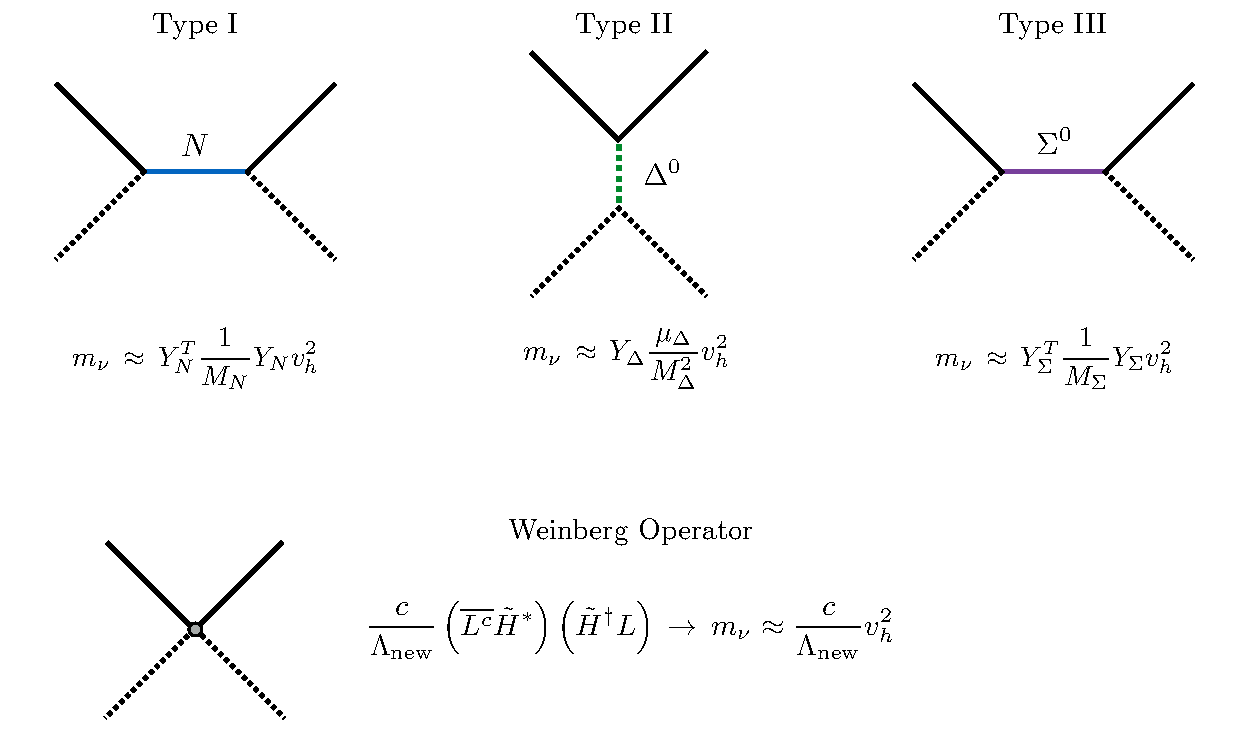
\includegraphics[width=\textwidth]{seesaw_mechanisms.pdf}
\caption[The tree-level UV completions of the Weinberg operator.]{The tree-level UV completions (top) of the $d=5$ Weinberg operator (bottom) with their respective contributions to light neutrino masses.\label{fig:seesaw_mechanisms}}
\end{figure}
%


\paragraph{Type I} The Lagrangian for this extension is precisely the one in \refeq{eq:typeILagrangian}. For convenience, let us work in the single generation case. We collect all mass terms into a single mass matrix of the form
%
\renewcommand{\arraystretch}{0.8}
\begin{equation}
  -\mathscr{L}_{\nu-{\rm mass}} \supset \frac{1}{2} \left( \begin{matrix}  \overline{\nu_L} & \overline{N^c} \end{matrix} \right) \left( \begin{matrix}  0 &  m \\ m & M_N \end{matrix} \right)  \left( \begin{matrix} \nu_L^c \\ N \end{matrix} \right) \,+\, {\rm h.c.},
\end{equation}
%
where $m = y^\nu_N v/\sqrt{2}$ and $M_N$ is the Majorana mass for $N$. Diagonalizing this mass matrix with a simple rotation $R(\theta)$, we find
%
\begin{equation}
 m_{1,2} = \frac{M_N \pm \sqrt{M_N^2 - 4m^2}}{2},\quad {\rm with}  \quad\tan{2 \theta} = \frac{2 m}{M_N}.
\end{equation}
%
In the so-called seesaw limit ($m \ll M_N$), this simplifies to 
%
\begin{equation}
 m_{1} \approx -\frac{m^2}{M_N} = \frac{(y^\nu_N v)^2}{2 M_N}, \quad m_2 \approx M_N  \quad {\rm with}, \quad \theta \approx \frac{m}{M_N},
\end{equation}
%
where the seesaw mechanism is in action: the large separation of scales between $m$ and $M_N$ explains the smallness of the light neutrino masses $m_1$. Saturating the upper bound on neutrino masses $m_1 \approx 0.1$ eV, we can infer that
\begin{equation}
 \left(y^\nu_N\right)^2 \approx 3 \times 10^{-15} \, \left(\frac{M_N}{{\rm GeV}} \right), \qquad \theta^2 \approx 10^{-10} \, \left(\frac{M_N}{{\rm GeV}} \right)^{-1}.
\end{equation}
%
Again, we conclude that the scale of new physics for couplings of $\mathcal{O}(1)$ lies at $M_N \approx 10^{15}$ GeV, in this case with very small mixing angles between the light states and the flavour $N$. Of course, this is only a naive scaling and becomes more complicated in the full three generation case~\cite{Casas:2001sr}. Nevertheless, it shows that heavy neutrinos at reasonably low scales are a reachable candidate to realise the seesaw mechanism, provided we are comfortable with small values for $y^\nu_N$.

\paragraph{Type II} In the presence of a scalar $\bm{\Delta}$, triplet under $SU(2)$, we can write
%
\begin{equation}\label{eq:typeIILagrangian}
 - \mathscr{L}_{\nu-{\rm mass}} \supset y^\nu_\Delta \, \overline{L^c} i\sigma_2 \bm\Delta L, \quad {\rm with}\quad \bm{\Delta} = \left( \begin{matrix} \Delta^+/\sqrt{2} & \Delta^{++} \\ \Delta^0 & -\Delta^+/\sqrt{2} \end{matrix} \right),
\end{equation}
%
where new charged scalars are appear. The scalar potential acquires the term
\begin{equation}
 -V(H,\Delta) \supset  \mu_\Delta H^T \,i\sigma_2\bm{\Delta} H + M_\Delta^2 \Tr{\bm{\Delta}^\dagger\bm{\Delta}},
\end{equation}
%
and is in general much more complicated. One can show that the neutral component acquires a vev $\langle \Delta^0 \rangle \approx \mu_\Delta v^2/M_\Delta^2$, where we ignored additional mixing terms between the Higgs and the new scalar degrees of freedom~\cite{Arhrib:2011uy}. This vev, then gives neutrinos mass through \refeq{eq:typeIILagrangian}, which interestingly, is linear in the neutrino Yukawa and suppressed by the typical mass scale of $\Delta$
%
\begin{equation}
 m_1 \approx y^\nu_\Delta  \frac{\mu_\Delta \,v^2}{M_\Delta^2}.
\end{equation}
%
The field $\bm{\Delta}$, in fact, carries lepton number $L=2$, and so the LNV parameter $\mu_\Delta$ being small is a technically natural choice. In this model, the vev of $\Delta^0$ is constrained to be very low, $\langle \Delta^0 \rangle \lesssim 5$ GeV, as $\bm{\Delta}$ contributes to the EW gauge boson masses through its kinetic term ${\rm Tr}\left[ (D_\mu \bm{\Delta})^\dagger (D^\mu\bm{\Delta}) \right]$. Finally, we can see for $m_1 \approx 0.1$ eV, we get
%
\begin{equation}
 y^\nu_\Delta \approx \left( \frac{1 {\rm eV}}{ \mu_\Delta}\right)  \, \left( \frac{M}{1 \,{\rm TeV}}\right)^2,
\end{equation}
%
suggesting a clear target for experimental searches around at EW scale.

\paragraph{Type III} The fermionic triplet couples to the doublets through
%
\begin{equation}\label{eq:TypeIII}
 - \mathscr{L}_{\nu-{\rm mass}} \supset y^\nu_\Sigma \, \overline{L} \bm{\Sigma} H, \quad {\rm with } \quad 
\bm{\Sigma} = \left( \begin{matrix} \Sigma^0 &  \Sigma^+/\sqrt{2} \\ \Sigma^-/\sqrt{2} & - \Sigma^0 \end{matrix} \right).
\end{equation}
%
In this case, the scalar sector may remain unchanged and the field $\Sigma^0$ behaves very similarly to the field $N$ in the Type I seesaw. Analogously to the Type I, we can write 
%
\begin{equation}
 m_1 \approx \frac{(y^\nu_\Sigma v)^2}{2 M_\Sigma}.
\end{equation}
%
This model is much less explored in the literature, but its phenomenology is quite rich. The term related to charged-leptons in \refeq{eq:TypeIII} induces charged-lepton mixing, and leads to rare processes such as $\mu\to e\gamma $ and $\mu \to e e e $ already at tree-level, contrary to the Type-I seesaw where they appear at one loop.

\subsection{Low-Scale Seesaw Variants} All of the previous models may be searched for at low or high energy ranges, but for large Yukawa couplings, are regarded as high-scale solutions to the neutrino problem. Exceptions to this arise in construction where additional symmetry arguments are at play. Most famous are the Inverse Seesaw (ISS)~\cite{Mohapatra:1986bd,GonzalezGarcia:1988rw} and the Linear Seesaw (LSS)~\cite{Wyler:1982dd,Akhmedov:1995ip,Akhmedov:1995vm}, where the lightness of neutrino masses is explained by an approximate conservation of lepton number, and the Extended Seesaw (ESS)~\cite{Kang:2006sn,Barry:2011wb,Zhang:2011vh}, where new hierarchies appear in the heavy sector. All these extensions arise from introducing a additional neutral fermions to the Type I seesaw particle content. In particular, in the single generation case, the most general mass matrix we can construct with the new fermions $N$ and $S$ is given by~\cite{LopezPavon:2012zg}
%
\begin{equation} \label{eq:typeIvariants}
   -\mathscr{L}_{\nu-{\rm mass}} \supset \frac{1}{2} \left( \begin{matrix}  \overline{\nu_L} & \overline{N} &  \overline{S} \end{matrix} \right) \left( \begin{matrix}  0 &  m & \epsilon \\ m & \mu^\prime & \Lambda  \\ \epsilon & \Lambda & \mu \end{matrix} \right)  \left( \begin{matrix} \nu_L^c \\ N^c \\ S^c \end{matrix} \right) \,+\, {\rm h.c.}
\end{equation}
%
Note that lepton number, defined as $L = L_e + L_\mu+L_\tau+L_N+L_S$, is violated by $\mu$, $\mu^\prime$ and $\epsilon$ if we assign, as usual, $L_N = - L_S$. From the diagonalization of this mass matrix, we learn that 
\begin{equation}
 m_1 = \frac{\mu m^2 - 2 \epsilon m\Lambda  + \epsilon^2 \mu^\prime }{\Lambda^2 - \mu \mu^\prime}.
\end{equation}
%
Therefore, we see that if all LNV parameters are set to zero, neutrino masses vanish. In the same way, if we set $\epsilon,\mu \to 0$, then we also get vanishing neutrino masses, at tree level. This accidental cancellation is very peculiar, and will be realised in the model introduced in Chapter 5. As it turns out, $\mu^\prime$ breaks lepton number, and so radiative corrections can be large, responsible for the light neutrino masses in this case. 

The ISS model can be recovered in the limit $\Lambda \gg m \gg \mu \gg \mu^\prime, \epsilon$. Now, the smallness of neutrino masses are controlled by the LNV parameter $\mu$, which is small due to approximate conservation of $L$, and suppressed by $1/\Lambda^2$, realising the seesaw mechanism. In this way, the additional neutrino states combine into a pseudo-Dirac pair, with a mass of $m_{2,3} \approx \Lambda \mp (\mu+\mu^\prime)/2$. These type of models predict small LNV, but the new heavy fermions will reside at much smaller scales while mainting the Yukawa couplings large. The LSS is another special case where $\Lambda \gg m \gg \epsilon \gg \mu^\prime,\mu$. In this case the light neutrino mass is \emph{linear} in $m$ and suppressed by $\epsilon/\Lambda^2$. 


In the ESS limit, $\mu^\prime \gg \Lambda, m \gg \mu, \epsilon$, LNV is large and the light neutrino masses are suppressed by the scale $\mu^\prime$. The seesaw, in this case, happens both for light and intermediate neutrinos, and so light new fermions are typical predictions of the model, of interest to the literature on scale sterile neutrinos.

% These models have been extensively studied in the framework of Minimal Flavour Violation (MFV)~\cite{Gavela:2009cd}, where the only source of flavour violation is assumed to be equal to that in the SM (through Yukawa couplings). 
%
\begin{figure}[t]
\centering
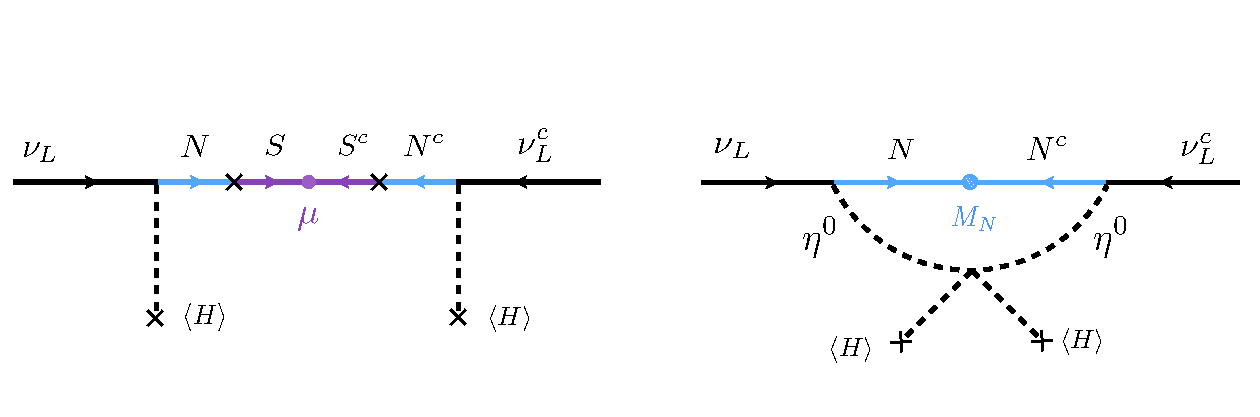
\includegraphics[width=\textwidth]{LNV_diagrams.pdf}
\caption[Diagrams for inverse seesaw and scotogenic model.]{On the left, the inverse seesaw flavour diagram for Majorana neutrino masses. On the right, the flavour diagram for the scotogenic mode. Arrows represent lepton number. \label{fig:LNVdiagrams}}
\end{figure}
%
\subsection{Radiative Masses}\label{sec:radiative}

A further possibility to generate the Weinberg operator is that Majorana neutrino masses arise from higher-order diagrams in perturbation theory. Since in the SM $L$ is an accidental symmetry, neutrino masses vanish at all orders, but this may not be the case in a generic SM extension. For instance, neutrino masses may arise at $n$ loops, in which case a naive estimate for the scale of new physics is
%
\begin{equation}
 \frac{c}{\Lambda} \approx  \left( \prod_{i}^\text{\# of vertices} g_i \right) \left(\frac{1}{4\pi}\right)^{2n} \frac{1}{M},
\end{equation}
%
where $g_i$ stand for the new couplings of the theory and $M$ is a new mass scale. The loop suppression factor is of interest since it lowers the scale $\Lambda$ without the need for small couplings or large masses. Many models for radiative neutrino masses exist, where typically new particles are introduced together with a new symmetry that prevents any of the mechanisms discussed previously to take place. 

The most illustrative example is perhaps the \emph{scotogenic} model~\cite{Ma:2006km}, sometimes also referred to as the radiative seesaw. Here, new SM singlet fermions $N$ are introduced together with $\eta$, a copy of the Higgs doublet with $\eta = (\eta^+, \eta^0\,)^T$ and $Y_\eta = Y_{H} = 1$. To forbid tree-level masses, an additional $Z_2$ discrete symmetry is introduced, under which all new states are odd ($N \to -N$ and $\eta \to -\eta$) and all SM particles are even (\eg, $L \to L$). In the single generation case, the new fermion mass terms are
%
\begin{equation}
-\mathscr{L}_{\nu-{\rm mass}} \supset \frac{M_N}{2} \overline{N^c} N + \left[y^N \left(\overline{L} \, \widetilde{\eta} \right) N \,+\, {\rm h.c.} \right],
\end{equation}
%
where the Yukawa term $(\overline{L} \widetilde{H}) N$ is not allowed by virtue of the $Z_2$ symmetry. The scalar potential now contains 
%
\begin{equation}
 V(H,\eta) \supset m_{\eta}^2 \eta^\dagger \eta + \frac{\lambda^\prime}{2} \left[ \left( H^\dagger \eta\right)^2 + \left( \eta^\dagger H \right)^2 \right],
\end{equation}
%
where $m_\eta^2 > 0$ and $\eta^0 = (\eta_R + i \eta_I)/\sqrt{2}$ acquires no vev. After SSB, we end up with an additional neutral scalar $\eta_R$ and neutral pseudo-scalar $\eta_I$ of masses $m_{R,\, I}^2 = m_\eta^2 \pm \lambda^\prime v^2/2$. The one-loop neutrino masses are then given by 
%
\begin{equation}
 m_1 = \frac{1}{2}\left(\frac{y^N}{4\pi}\right)^2 M_N \left[ \frac{m_R^2}{m_R^2 - M_N^2 } \ln \left( \frac{m_R^2}{M_N^2} \right) - \frac{m_I^2}{m_I^2 - M_N^2 } \ln \left( \frac{m_I^2}{M_N^2} \right) \right].
\end{equation}
%
In this case, we can see the loop suppression and the new Yukawas. To find what mass scale appears in the denominator, we may choose a limit. For $M_N \gg m_\eta$, we find $m_1 \propto \lambda^\prime v^2/M_N$ up to loop factors and the Yukawas, while for $M_N \ll m_\eta$, we have $m_1 \propto \lambda^\prime v^2 M_N/m_\eta^2$. The diagram on the right in \reffig{fig:LNVdiagrams} explicitly shows how this dependence comes about. 

Note that due to the $Z_2$ symmetry, $N$ and $\eta^0$ define a dark sector, with the lightest particle being a DM candidate. Despite the absence of the neutrino portal operator in this case, neutrino mixing between light states and the flavour $N$ is generated at one loop. In addition, the $\eta^\pm$ provides a strong connection between the SM and the dark sector. Many models for radiative neutrino masses display similar features to these, where new dark states often solve the neutrino and DM puzzle at the same time. This connection is explored in more detail in Chapter 5. Beyond one loop, neutrino mass models have been studied up to three-loop level~\cite{Krauss:2002px}.

\section{Neutrino Mixing} Now that we have a series of concrete models to generate neutrino masses, we would like to understand the consequences of massive neutrinos at low energies and how we learned about their mass. For our current purposes, we will focus purely on the $SU(2)$ breaking operator for Majorana and Dirac neutrino masses
%
\begin{equation}\label{eq:lowEmasses}
 \mathscr{L}_{\nu-{\rm mass}}^{\rm M} = \frac{M_{\alpha \beta}}{2} {\overline{\nu_L^c}^\alpha \nu_L^\beta} \,+\, {\rm h.c.,} \qquad %
 \mathscr{L}_{\nu-{\rm mass}}^{\rm D} = \frac{y^\nu_{\alpha \beta} v}{\sqrt{2}} \,{\overline{\nu_L}^\alpha N^\beta} \,+\, {\rm h.c.,}
\end{equation}
%
where the former Lagrangian describes purely Majorana neutrinos, and the latter describes purely Dirac neutrinos with the addition of three $N$ states to the SM. We will work with only three $N$ states for simplicity, any number greater than two is analogous. Similarly to the quark sector, we would like to diagonalize these mass matrices and find the relevant mixing matrix. We proceed with the two cases in parallel and start by rotating all fields independently with unitary matrices
%
\begin{align}
\nu_L^\alpha \to U^\nu_{\alpha k} \nu_L^k, \qquad & N^\alpha \to V^\nu_{\alpha k} N^k \nonumber\\
 e_L^\alpha \to U^e_{\alpha k} e_L^k,\qquad & e_R \to V^e_{\alpha k} e^k,
\end{align}
%
where $U$ ($V$) rotates LH (RH) fields. From \refeq{eq:lowEmasses}, it is clear that the diagonalization is slightly different in the two cases. The diagonal mass matrices are 
%
\begin{equation}
\textbf{M} \to \hat{\textbf{M}} = \textbf{U}^{\nu\,T} \textbf{M} \textbf{U}^\nu, \qquad   \textbf{Y} \to \hat{\textbf{Y}} = \textbf{U}^{\nu\,\dagger} \textbf{Y} \textbf{V}^\nu,
\end{equation}
%
where $\textbf{M}$ and $\textbf{Y}$ are diagonal matrices~\footnote{Note that in the Dirac case, the mass matrix $\textbf{Y}$ is diagonalized by its singular value decomposition, and in the Majorana case we assumed $\textbf{M}$ to be complex \emph{symmetric} and the special case of Takagi factorization applies.}. The CC Lagrangian defines lepton mixing through the Pontecorvo-Maki-Nakagawa-Sakata (PMNS) matrix~\cite{Pontecorvo:1957qd,Maki:1962mu}
%
\begin{equation}
\overline{e_L}^\alpha \gamma_\mu P_L \nu_L^\alpha \to \overline{e_L}^k P_L \, \left(U_{\rm PMNS}\right)_{kj} \,\nu_L^j, \qquad \textbf{U}_{\rm PMNS} = \textbf{U}^{e\,\dagger} \textbf{U}^\nu.
\end{equation}
%
At this point, we can identify the charged-lepton fields $e^k$ with their gauge basis (\ie, their flavour and mass basis coincide $\alpha \sim k$) and define the LH flavour neutrino field $\widehat{\nu}^\alpha = \left(U_{\rm PMNS}\right)_{\alpha j} \nu_L^j$. This is the relevant field for all neutrino CC interactions, but it does not have a well-defined mass. For simplicity, we will now adopt the notation $\widehat{\nu}^\alpha \equiv \nu^\alpha$.
%
\begin{figure}[t]
\centering
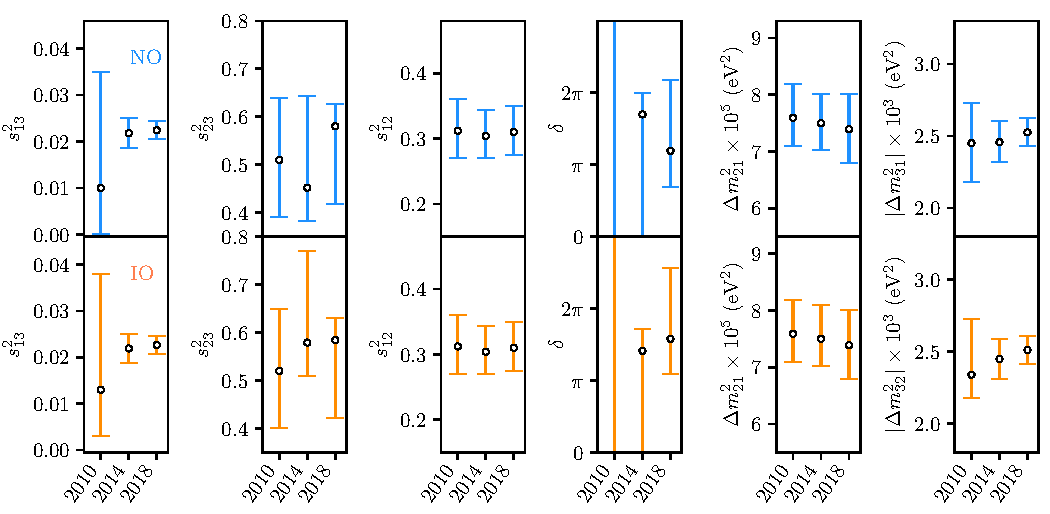
\includegraphics[width=\textwidth]{plots/precision2.pdf}
  \caption[Oscillation global-fit comparison between 2010, 2014 and 2018 datasets.]{The neutrino oscillation global-fit results in 2010~\cite{Schwetz:2011qt}, 2014~\cite{Gonzalez-Garcia:2014bfa} and 2018~\cite{Esteban:2018azc}. We show the best-fit point, together with the $3\sigma$ regions for normal ordering (NO) and inverted ordering (IO).\label{fig:measurements}}
\end{figure}
%

The PMNS mixing matrix is responsible for neutrino mixing and its entries are model dependent, arising from the flavour structure of the neutrino Yukawas and Majorana masses. In the general case, it is parametrized by
\renewcommand{\arraystretch}{0.9}
\begin{align}\label{eq:neu:UmixFull}
U_{\rm PMNS}&= \left(
\begin{matrix}
1 & 0        & 0\\
0 & c_{23}   & s_{23}\\
0 & -s_{23}  & c_{23}\\
\end{matrix}
\right)\hspace{-1ex}\left(
\begin{matrix}
c_{13}              & 0  & s_{13}e^{-i\delta} \\
0                   & 1  & 0                  \\
-s_{13}e^{-i\delta} & 0  & c_{13}             \\
\end{matrix}
\right)\hspace{-1ex}\left(
\begin{matrix}
c_{12}  & s_{12} & 0 \\
-s_{12} & c_{12} & 0 \\
0       & 0      & 1 \\
\end{matrix}
\right) D, 
% \hspace{-1ex}\left(
% \begin{matrix}
% 1               & 0                 & 0 \\
% 0               & e^{i\alpha_2/2} & 0 \\
% 0               & 0                 & e^{i\alpha_3 / 2}
% \end{matrix}
% \right),
% \nonumber\\
% &=\left(
% \begin{matrix}
% U_{e 1}& U_{e 2}  & U_{e 3}\\
% U_{\mu 1} & U_{\mu 2} & U_{\mu 3}\\
% U_{\tau 1} & U_{\tau 2} & U_{\tau 3}\\
% \end{matrix}
% \right),
\end{align}
%
where $c_{ij} = \cos{\theta_{ij}}$ and $s_{ij}= \sin{\theta_{ij}}$ are the cosine and sine of the mixing angles to be measured from oscillation data. The matrix $D = {\rm diag}\{1,e^{i\alpha_2/2}, e^{i\alpha_3/2}\}$ contains additional phases that are physical when neutrinos are Majorana. As we will see in the next section, oscillation data can shed light on all mixing angles, mass-squared differences $m^2_{ij} = m_i^2 - m_j^2$, and on the CP-violating phase $\delta$. Neutrino oscillations are insensitive, however, to any Majorana phases.

Immense efforts to measure all parameters in the PMNS have been carried out in the past 26 years. In \reffig{fig:measurements}, we show the relative precision reported by a global-fit to neutrino oscillation data, comparing the data release from after the Neutrino conferences of 2010~\cite{Schwetz:2011qt}, 2014~\cite{Gonzalez-Garcia:2014bfa} and 2018~\cite{Esteban:2018azc}. All three mixing angles and two mass-squared splittings have been succesfully measured to at least $3\sigma$, with the exception of the CP-violating phase $\delta$, which is still largely unknown. Another interesting development is our knowledge of the mass ordering. This is a measurement of the sign of $\Delta m^2_{3\ell}$, where $\ell = 1$ for normal ordering (NO) and $\ell = 2$ for inverted ordering (IO). While currently the global-fit in Ref.~\cite{Esteban:2018azc} displays a mild preference for NO ($\Delta \chi^2 = 4.7$), future measurements are needed. For $\Delta m^2_{21}$, this sign is known, as it strongly impacts the matter potential of solar neutrinos.


\subsection{Neutrino Oscillations}

Neutrino oscillations arise when a superposition of neutrino mass eigenstates is produced, propagates macroscopic distances and scatters inside a detector. Given sufficiently long baselines, neutrino flavour transitions may always occurs due to mixing, but for a non-trivial dependence on baseline distances, coherence must be preserved throughout the process. In this section, we will make these statements more precise and derive the standard formula for the oscillation probability $P(\nu_\alpha \to \nu_\beta)$ in vacuum (matter effects are discussed in \refsec{sec:matter_effects}). This exercise can be done in multiple ways and most often derivations rely on plane-wave neutrino states. This approach leads to correct expressions for $P(\nu_\alpha \to \nu_\beta)$ in virtually all cases of interest, but it is a rather poor conceptual description of oscillations and relies on unphysical assumptions. Instead, we will derive the oscillation formula from a quantum mechanical wave packet approach, and encounter a few conditions for oscillations to happen. More sophisticated treatments in Quantum Field Theory (QFT), often called the \emph{external} wave packet approach, have been known for some time~\cite{Cardall:1999ze,Beuthe:2001rc,Giunti:2002xg}, and their results have been shown to be directly mapped onto the \emph{internal} wave packet approach~\cite{Akhmedov:2010ms} we discuss here. Nonetheless, neutrino oscillations are notorious for being conceptually confusing and the correct method to compute such processes is still debated in the literature~\cite{Kobach:2017osm}. We may seek consolation in the fact that a few aspects are common to all approaches, for instance, the ultra-relativistic nature of the mass states through expansions of $\sqrt{m^2 + p^2}$ and the need for momentum uncertainties in the initial and final neutrino processes.
%
\begin{figure}[t]
\centering
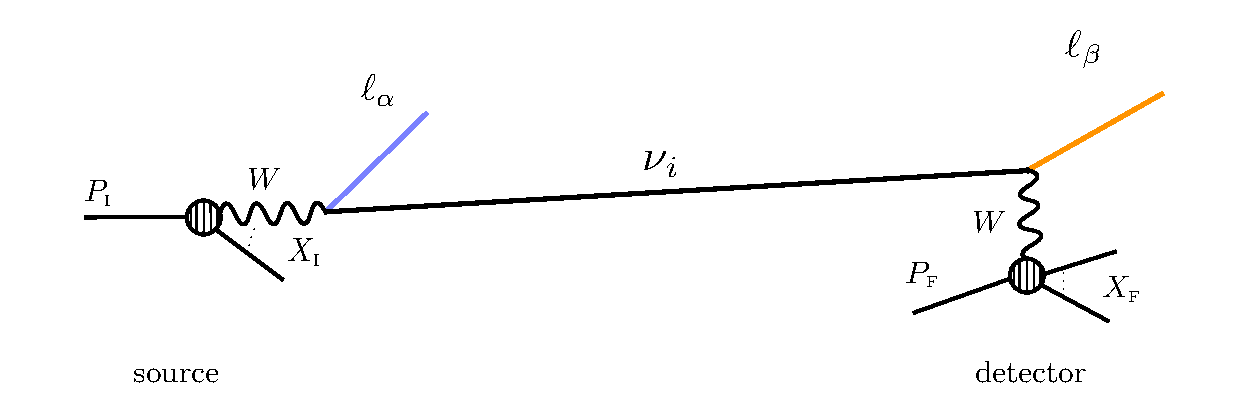
\includegraphics[width=\textwidth]{oscillations_diagram.pdf}
  \caption[Neutrino oscillations diagram.]{The usual set-up of an oscillation experiment. We show the source, where a process $P_\textsc{i} \to \nu_\alpha \, X_\textsc{i}$ happens (note that $P_\textsc{i}= \ell_\alpha$ is allowed and that $P_\textsc{i}$ may be a scattering process), and the detector, where $\nu_\beta \,P_i \to \ell_\beta \,X_\text{f}$. \label{fig:oscillations_diagram}}
\end{figure}
%

Our setup typical of neutrino oscillations experiments and is represented in \reffig{fig:oscillations_diagram}. We will first discuss the role of production and detection processes, and then later study the oscillations \emph{per se}. Initially, a neutrino flavour state $\nu_\beta$ is produced in a CC reaction at the source, $P_\textsc{i} \to \nu_\beta X_\textsc{i}$. More precisely, a state $\ket{f}$ is produced,
%
\begin{equation}\label{eq:flavour_source}
 \ket{f} = \hat{S} \ket{P_\textsc{i}}, \quad \hat{S} \approx  \hat{1} - i \int \dd^4 x \, H_{\rm int}^{\rm CC} (x),
\end{equation}
%
where $\hat{S}$ is the S-matrix operator approximated to first order in weak coupling and
%
\begin{equation}
 H_{\rm int}^{\rm CC} (x) = \sqrt{2} G_F\, \sum_\alpha \overline{\nu}_\alpha (x) \gamma^\mu P_L \ell_\alpha(x) \, J_\mu (x) \,+\, {\rm h.c.},
\end{equation}
%
is the interaction Hamiltonian between the neutrino current and the current $J_\mu(x)$ that describes the transition $P_\textsc{i} \to X_\textsc{i}$. After $\ell_\alpha$ and the final particles interact with the medium, $\ket{f}$ is projected out onto the state $\bra{\ell_\alpha,\,X_\textsc{i}}\ket{f}$, which ought to ensure that the neutrino state produced is a superposition of massive states weighed by the PMNS matrix elements $U_{\alpha i}^*$ and other kinematic factors. Note that this may differ from the usual definition of a flavour state $\ket{\nu^\alpha} = U_{\alpha i}^* \ket{\nu_i}$, which can be misleading in this situation as these do have a definite mass and do not span a Fock space (for a recent and illuminating discussion on this issue, see Ref.~\cite{Cozzella:2018zwm}). We want to work instead with the eigenstates of the free Hamiltonian, which are the ones with a definite mass and that can easily be evolved in time. With this in mind, we define the following amplitude
%
\begin{equation}
 A_{\alpha k}(\vec{p},h)^P \equiv \bra{\nu_k(\vec{p},h),\ell_\beta,X_{\textsc{i}}} \hat{S}\ket{P_\textsc{i}}, \quad {\rm with} \quad A_{\alpha k}(\vec{p},h) = U^*_{\alpha k} M_{\alpha k}(\vec{p},h),
\end{equation}
%
where we factored out a mixing angle in the definition of $M_{\alpha k}$ and made the helicity index $h$ explicit. By virtue of the completeness relation with massive neutrino eigenstates, we can insert the identity in $\bra{\ell_\alpha,\,X_\textsc{i}}\ket{f}$ and define a \emph{normalized} neutrino flavour state as
%
\begin{equation}
 \ket{\nu_\alpha}^P = N_P \,\sum_{k, h} \, \int \dd^3 p\, A^P_{\alpha k} (\vec{p},h) \ket{\nu_k(\vec{p},h)}, \quad N_P^{-2} = \sum_{k,h} \int \dd^3 p \, \left|A^P_{\alpha k} (\vec{p},h)\right|^2.
\end{equation}
%
An analogous discussion holds for the detection process $\nu_\beta \, P_\textsc{f} \to \ell_\beta \, X_\textsc{f}$, where a detection flavour state $\ket{\nu_\alpha}^D$ with an amplitude for detection $A_{\alpha k}(\vec{p},h)^D$ can be defined. Before we move on to a discussion about oscillations, we want to emphasize two points. First, the normalization of the flavour state is a clear sign that we are working in a quantum mechanical description. To compute probabilities, we rely on normalized states. In a QFT description, however, the normalization is not necessary, but neither is the concept of $P_\textsc{i} \to X_\textsc{i}$ in the first place. There, the full process $P_\textsc{i} \, P_\textsc{f} \,\to\, X_\textsc{i}\, X_\textsc{f}\, \ell_\alpha \, \ell_\beta$ in \reffig{fig:oscillations_diagram} can be compute directly through the use of long-distance propagators. If the production, propagation and detection parts of the amplitude squared factorize, an object analogous to the oscillation probability can be extracted. This factorization is implicitly assumed in our calculation. Secondly, the decay rate of the $P_\text{I}$ particle can be computed as
%
\begin{equation}
 \left|A^P\right|^2 =  \left|  \bra{\nu_\alpha (\vec{p},h),\ell_\beta, X_{\textsc{i}}} \hat{S} \ket{P_\textsc{i}}  \right|^2 = \sum_{k,h} \,|U_{\alpha k}|^2\, \int \dd^3 p \, \left|M^P_{\alpha k} (\vec{p},h) \right|^2,
\end{equation}
%
and it becomes evident that the decay rate is given by the \emph{incoherent} sum of the decay rate into different massive neutrinos. No interference is present as the states $\ket{\nu_k}$ are assumed to be orthonormal to each other. This remains true in the QFT description~\cite{Giunti:2002xg}.

Now, one is left to compute the functions $M_{\alpha k}$. This is a rather involved process, but one can show that the form of these functions resemble simple wave packets~\cite{Akhmedov:2010ms}. In doing so, many approximations are necessary, in particular, that of ultra-relativistic neutrinos. More precisely, the most relevant assumptions are \emph{i)} flipped-helicity terms ($h=+1$ for neutrinos), suppressed by $m_k^2/E_k^2$, are ignored, \emph{ii)} all neutrinos travel in the same direction, $\vec{p} \to p$, and \emph{iii)} the production and detection processes are not sensitive to the neutrino mass differences, amounting to replacing $M_{\alpha k} \approx M_\alpha$. Under these assumptions, we are justified to take normalized gaussian wave packets for production and detection flavour states as an \emph{ansatz},
%
\begin{equation}
 \ket{\nu_\alpha}^i =  \sum_{k}  U^*_{\alpha k} \, \int \dd p \, \psi_k^i (p) \,\ket{\nu_k({p})}, \quad%
 %
 \psi_k^i (p) = \left(2\pi\,\sigma_p^{i\, 2}\right)^{-1/4} \exp\left[ - \frac{(p-p_k)^2}{4 \sigma_p^{i\, 2}} \right],
\end{equation}
%
with $\sigma_p^i$ being the spread around the central momenta $p_k$ and $i=P,D$.

Now that the flavour states are written in terms of the eigenstates of the free Hamiltonian, we know how to evolve them and how to write the flavour transition amplitude after a time $t$ and distance $L$
%
\begin{align}
 A(\nu_\alpha \to \nu_\beta) &= \bra{\nu_\beta^D} e^{-i \hat{E} t + i \hat{P} L} \ket{\nu_\alpha^P}
 \nonumber \\ &= N \,\sum_k U_{\alpha k}^* U_{\beta k} \int \dd p \exp\left[ -i E_k(p) t + ip L - (p -p_k)^2/4 \sigma_p^2\right],
\end{align}
where $E_k(p) = \sqrt{p^2 + m_k^2}$ and $N$ is a normalization factor coming from the normalization of the wave packets and a single integral over $p$. We have also defined the global uncertainty on momentum $\sigma_p^{-2} = \left(\sigma_p^{P}\right)^{-2} + \left(\sigma_p^{D}\right)^{-2}$. This may also be related to the global uncertainty on production and detection positions through $\sigma_x \sigma_p \approx 1/2$. Finally, to integrate over the remaining $p$ integral, we can Taylor expand around the central wave packet momentum
%
\begin{equation}
 E_k(p) \approx E_k + v_k (p-p_k), \quad{\rm with}\quad v_k = \left.\frac{\partial E_k(p)}{\partial p}\right|_{p=p_k} = \frac{p_k}{E_k},  \quad E_k = \sqrt{p_k^2 + m_k^2}.
\end{equation}
%
Performing the final integral over $p$, integrating over $t$ (an unmeasured quantity) and squaring the amplitude, one obtains a formula for the oscillation probability
%
\begin{equation}
 P(\nu_\alpha \to \nu_\beta) = \sum_{k,j} U_{\alpha k}^*U_{\alpha j}U_{\beta k}U_{\beta j}^* \, e^{-2\pi i L/L^{\rm osc}_{kj}} \, P^{\rm coh}_{kj} \, P^{\rm loc}_{kj},
\end{equation}
%
where we defined
%
\begin{equation}
  P^{\rm loc}_{kj} = \exp\left( -2 \pi^2 \xi^2 \left(\frac{\sigma_x}{L_{kj}^{\rm osc}} \right)^2 \right),\quad  P^{\rm coh}_{kj} = \exp\left( \frac{L \left|\Delta m^2_{kj} \right|^2}{16 E^2 \sigma_x} \right),
\end{equation}
%
with the important scales of the problem identified as
%
\begin{equation}
 L_{kj}^{\rm osc} = \frac{4 \pi E}{\Delta m_{kj}^2}, \quad  p_k \approx E - (1-\xi) \frac{m_k^2}{2E}, \quad E_k \approx E + \xi \frac{m_k^2}{2E},
\end{equation}
with $\xi$ measuring the deviation from ultra-relativistic behaviour. The factors $P^{\rm coh}_{kj}$ and $P^{\rm loc}_{kj}$ are related to the coherence of the propagating wave packets and the localization of the source (or detector), respectively.
%

For most applications, $P^{\rm coh}_{kj} = P^{\rm loc}_{kj} = 1$, and one recovers the standard oscillation formula. A more useful way of writing it is
%
\begin{align}
 P(\nu_\alpha \to \nu_\beta) =
 \delta_{\alpha\beta} &- 2\sum_{k>j} \Re{U_{\alpha k}^*U_{\alpha j}U_{\beta k}U_{\beta j}^*} \left[ 1- \cos\left( \frac{\Delta m^2_{kj} L}{2E}\right) \right] \nonumber\\
 %
 &- 2\sum_{k>j} \Im{U_{\alpha k}^*U_{\alpha j}U_{\beta k}U_{\beta j}^*} \sin \left( \frac{\Delta m^2_{kj} L}{2E}\right).
\end{align}
%
Note that for very small distances, $L/E\to0$, no oscillations happen, $P(\nu_\alpha \to \nu_\beta) = \delta_{\alpha\beta}$. For very large $L/E \to \infty$, the oscillatory arguments are large and the oscillations are averaged out, although flavour transitions are still allowed. 

\subsection{Matter Effects}\label{sec:matter_effects}

Neutrinos are neutral particles and their rare interactions allow them to propagate through matter without losing energy in collisions with the medium particles. Nevertheless, in a similar fashion to photons, neutrinos undergo coherent forward scattering, acquiring an effective refractive index in the presence of a medium. In contrast to photons, which undergo Compton scattering, neutrinos are only charged under the weak force and undergo CC and NC interactions. Therefore, matter effects are present whenever the medium displays a net weak charge, provided by neutrons, protons and electrons in the case of the Earth. The weakness of these interactions at low energies, however, implies that matter effects are only important when neutrinos have transversed sufficiently large distances or are in a sufficiently dense environment. In addition, for such effects to be observable in the flavour evolution of neutrinos, different neutrino flavour fields must exhibit different interactions with the medium. In the SM, this is possible only due to the CC interactions that are exclusively present between electron-neutrinos and electrons in the medium.

We will now comment on the impact of matter in the flavour evolution, and derive the neutrino interaction potential. We want to avoid the complications from the previous discussion due to coherence and focus on the effects of matter. We merely note that similar conditions to the ones we found in the previous section apply for oscilation probabilities in matter to be well-defined, and with this caveat we proceed with a plane-wave picture of the flavour evolution. By applying the same momentum approximation and assuming neutrinos to be relativistic, we can write the Schr\"oedinger equation in matrix form as 
%
\begin{equation}\label{eq:matter_evolution}
 i \frac{\dd}{\dd x} \ket{\nu_\alpha} = \left[ U \frac{\hat{m}^2}{2E} U^\dagger + \hat{V}(x) \right] \ket{\nu_\alpha}, 
\end{equation}
%
where we used $H_0 \ket{\nu_\alpha} \approx U \left[ p \hat{1} + \hat{m}^2/2 p \right] U^\dagger \ket{\nu_\alpha} $ and $t \approx x$. Here, $\hat{V}(x)$ is a matrix containing the interaction potential of each neutrino flavour with the background. Note that $\hat{V}(x)$ depends on the density profile of matter particles. Solving this equation is a much more complicated task than in the vacuum case and analytical solutions are only known in specific cases, such as when the matter density is constant. In general, this may be solved numerically for a given choice of $\hat{V}(x)$, although several perturbative expansions exist. In this sense, the problem reduces to finding the appropriate potential and solving \refeq{eq:matter_evolution}.

The neutrino matter potential arises from finite temperature and finite density corrections to the neutrino dispersion relation. The derivation of the potential following the approach of Refs.~\cite{Notzold:1987ik,Nieves:1989ez} can easily be modified to early Universe physics and to exotic astrophysical media such as supernovae and environments with large magnetic fields. The dispersion relation arises from
%
\begin{equation}
 \det{\slashed{k} - \Sigma} = 0,
\end{equation}
%
ensuring non-trivial solutions to the Dirac equation $(\slashed{k} - \Sigma)\nu_L = 0$, with $k^\mu$ the neutrino four-momentum and $\Sigma$ its self-energy. For LH neutrino states $\nu_L$, we can write the neutrino self-energy in the most general form and make explicit the background dependent contribution as~\cite{Weldon:1982aq}
%
\begin{equation}
  \Sigma = m - \left( a_L \slashed{k} + b_L \slashed{u} + c_L [\slashed{k},\slashed{u}] \right) P_L.
\end{equation}
%
where $u$ is the 4-velocity of the medium, $a_L$, $b_L$ and $c_L$ are scalar functions of Lorentz invariants $w=k \cdot u$ and $\kappa=(w^2 - k^2)^{1/2}$, and $m$ is the vacuum neutrino mass. The presence of the medium introduces a preferential frame, namely the rest frame of the medium with $u = (1,0,0,0)$. Also note that in vacuum, only terms proportional to $\slashed{k}$ exist, and the pole of the neutrino propagator is unchanged. To lowest order in $g^2/m_\textsc{w}^2$, only $b_L$ contributes and it is proportional to the medium particle-antiparticle asymmetry. Higher order terms of the form $g^2/m_\textsc{w}^4$~\cite{DOlivo:1992lwg} complicate the picture, but can be safely neglected in the Earth, for instance. The neutrino self-energy is, in fact, a gauge-dependent quantity, and the physical observables of interest are the dispersion relations, $(1-a_L)(w-\kappa)- b_L = 0$ for neutrinos and $(1-a_L)(w+\kappa) - b_L = 0$ for antineutrinos. To lowest order, however, the dispersion relations are much simpler,
%
\begin{equation}
 w \approx \kappa + \frac{m^2}{2\kappa} + V_{\rm eff}, \quad V_{\rm eff} = -b_L,
\end{equation}
%
where we defined the effective potential, which for ultra-relativistic neutrinos arises precisely from the difference between the total and kinetic energy $V_{\rm eff} = w - \kappa$. This also shows us how to calculate the neutrino refractive index $n =\kappa/w$.
%
\begin{figure}[t]
 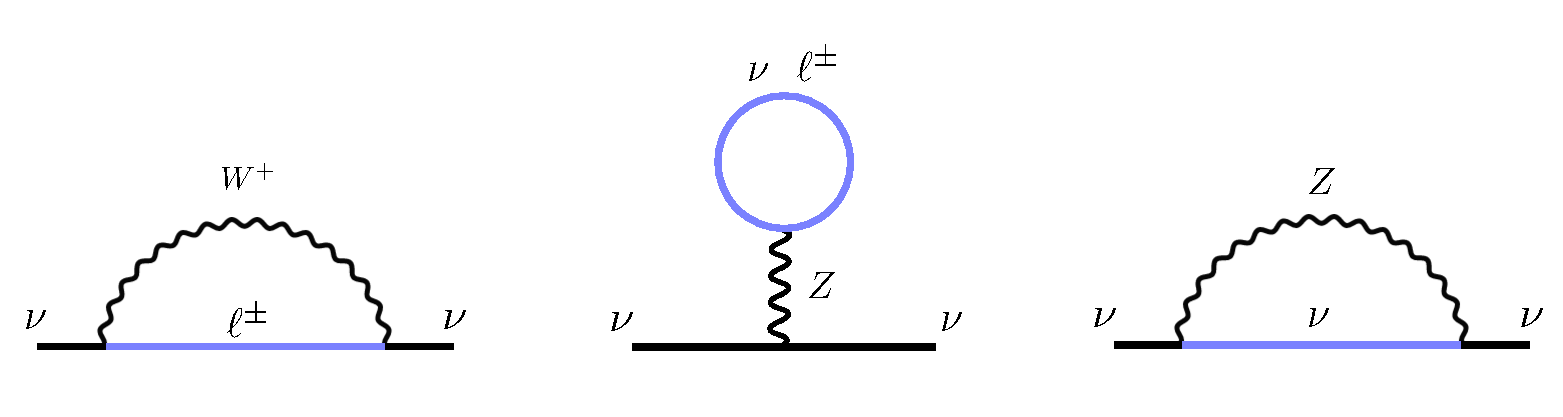
\includegraphics[width=\textwidth]{thermal_diagrams.pdf}
  \caption[Finite temperature corrections to $\Sigma$.]{Finite temperature and density corrections to the neutrino self-energy. These can be used to infer the effective matter potential for neutrinos.\label{fig:thermal_diagrams}}
\end{figure}

Now the problem reduces to computing $\Sigma$ in finite temperature field theory. For most applications of thermal mass calculations, replacing vacuum propagators by the thermal propagators from the real-time formalism is sufficient. In particular, the fermion thermal propagator of interest is
%
\begin{equation}
 S(P) = (\slashed{p} + m)\left[ \frac{1}{P^2 - m^2 +i\epsilon } + i 2\pi \delta(P^2 - m^2) f(P)\right],
\end{equation}
%
with $f(P) = \left\{ \exp\left[(|P\cdot u| - {\rm sgn}(P \cdot u) \,\mu_f)/T\right] + 1\right\}^{-1}$ is the occupational number of the fermions in the thermal bath of temperature $T$ and chemical potential $\mu_f$. Similar expressions exist for bosonic propagators. Finally, as an example, explicit computation of the tadpole self-energy contribution in \reffig{fig:thermal_diagrams} yields
%
\begin{equation}
 \Sigma = -i \frac{g^2}{16 c_\textsc{w}^2}\int \frac{\dd^4 P}{(2\pi)^4} \gamma^\mu P_L \,iS(P+K) \,\gamma^\nu \, P_L \,iD_{\mu\nu} (P),  \quad D_{\mu\nu} = \frac{-g_{\mu\nu} + \frac{P_\mu P_\nu}{M_Z^2}}{P^2 - M_Z^2 + i\epsilon}.
\end{equation}
%

By explicit computation in the rest frame of the medium, the potential for neutrinos of flavour $\alpha$ on a zero-temperature background of protons, neutrons and electrons is
%
\begin{align}
 V^e_\alpha =& -\frac{G_F}{\sqrt{2}} \left( 1-4s^2_\textsc{w} - 2\delta_{\alpha e}\right) \left( N_e - N_{\overline{e}} \right),\nonumber\\%
 V^p_\alpha =& \frac{G_F}{\sqrt{2}} \left( 1-4s^2_\textsc{w} \right) \left( N_p - N_{\overline{p}} \right),\nonumber\\%
 V^n_\alpha =& -\frac{G_F}{\sqrt{2}} \left(N_n - N_{\overline{n}} \right),
\end{align}
%
where $N_f = 2 \int \dd^3P f(P)/(2\pi)^3 $ are the number density of the background particles. For antineutrino an overall minus sign is introduced. Note the total $\nu_e$ potential is the only one where CC interactions contribute, and so it is the sole responsible for non-trivial flavour evolution in \refeq{eq:matter_evolution}. One may wonder about radiative corrections to these potentials in the SM and whether additional flavour non-universality can be achieved through the difference in charged-lepton masses. These effects, however, are known to be extremely small in the SM~\cite{Botella:1986wy}, where $\left(V_\tau - V_\mu\right)/V_e \approx 5 \times 10^{-5}$ for a neutral unpolarized medium like the Earth. 


\section{Neutrinos in the Laboratory}

To find a source of neutrinos, all we have to do is to look for environments where the weak force is prominently manifested. Natural candidates are nuclear reactors, having played a crucial role in the discovery of the neutrino. Fortunately, the list does not stop there. Abundant neutrino sources include the Sun, the atmosphere, the Big-Bang, particle accelerators and more violent astrophysical environments such as supernovae, active galactic nuclei and others. In this thesis, we will focus mostly on accelerator neutrinos.

Accelerator experiments typically produce neutrinos with energies of a few GeV to achieve $\mathcal{O}(1)$ oscillation phases $\Delta m^2_{\rm atm} L/E$ within thousands of km. Drastically different energy regimes are impractical either due to diluted fluxes at longer baselines ($\Phi \propto 1/L^2$), or due to thresholds to produce muons in CC interactions ($E_\nu > m_\ell + m_\ell^2/2 m_{\mathcal{H}}$ in reactions of the type $\nu_\ell \mathcal{H} \,\to\, \ell^\pm \mathcal{H}^\prime$). Proton beams with multi-GeV energies are used to produce neutrinos through the following steps: the protons are directed onto a dense target, the charged mesons produced in the proton-on-target collisions are focused with magnetic fields into a decay pipeline, and charged particles are absorbed further down the line. This allows the mesons to decay into neutrinos, most often through $\pi^\pm \to \overset{(-)}{\nu_\mu}\, \mu^\pm$. These experiments produce neutrinos within a wide range of energies, giving rise to wide-band beams. The shape and normalization of the neutrino flux produced are hard to model due to hadro-production and focusing uncertainties~\cite{Aliaga:2016oaz}. This comes mainly from the difficulty in describing hadron-nucleus interactions, their attenuation in propagation and, ultimately, by lack of data. In this way, the expected neutrino event rate in neutrino detectors inherits two sources of uncertainties which are difficult to disentangle: the unoscillated flux spectra and the neutrino-matter cross sections. 

For oscillation physics, however, one is only interested in disentangling uncertainties in the event rate and the effects of oscillations. One effective method to achieve this is to build near detectors, where unoscillated rate is measured, as well as far detectors, where oscillations have developed. By definition, near detectors have to be limited by the systematics of the experiment, and so require a large number of neutrino interactions. These are dominated by the processes shown in \reffig{fig:interactions_diagram} and their NC analogues. Because these processes are often subject to large nuclear effects (see below), other cleaner probes, such as neutrino-lepton scattering offer a better probe of the weak interactions in isolation. This argument will be essential when we search for \emph{stronger than weak} neutrino interactions (new interactions with 4-Fermi coupling constants with $G_X > G_F$). 
%
\begin{figure}[t]
\centering
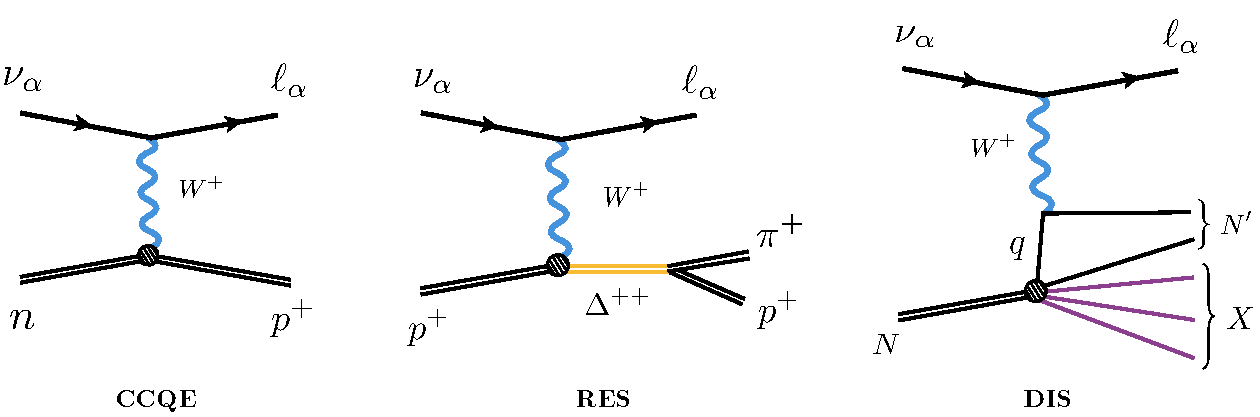
\includegraphics[width=\textwidth]{interactions.pdf}
  \caption[Neutrino nucleon interactions.]{The CC neutrino-nucleon scattering relevant for GeV neutrinos.From left to right, the CC quasi-elastic (CCQE), resonant (RES) and deep-inelastic scattering (DIS) regimes. Analogous diagrams exist for NC scattering. \label{fig:interactions_diagram}}
\end{figure}
%

\subsection{Interactions and Challenges}

Despite interacting exclusively through the weak force, when the neutrino scatters on a target nucleus, the visible final states are subject to the influence of the nuclear force. Opting for dense materials with large nuclei is preferred for oscillation physics, but as more precision is required in oscillation measurements, more control over the nuclear effects is needed. The near and far measurements of the neutrino flux helps in reducing systematics, but the neutrino flux at the near site is different from the oscillated flux at the far site, both in shape and in flavour composition. In this way, understanding how nuclear effects and neutrino cross sections depend on neutrino energy $E_\nu$ and neutrino flavour is of great importance. Let us comment on a few examples. Even in the crudest approximation for a nucleus, that of a $T=0$ Fermi gas of free protons and neutrons, nucleon final states are Pauli blocked and the occupation number of these fermions suppresses the total cross section. For realistic nuclei, these nucleons also display Fermi motion with momenta in the rest frame of the nucleus, $|p_N| \lesssim 250$ MeV, that are comparable to the incoming neutrino energy. On their way out of the nucleus, struck nucleons may also exchange EM charge, knock-out additional particles or be absorbed by the nuclear medium. 
%
\begin{figure}[t]
\centering
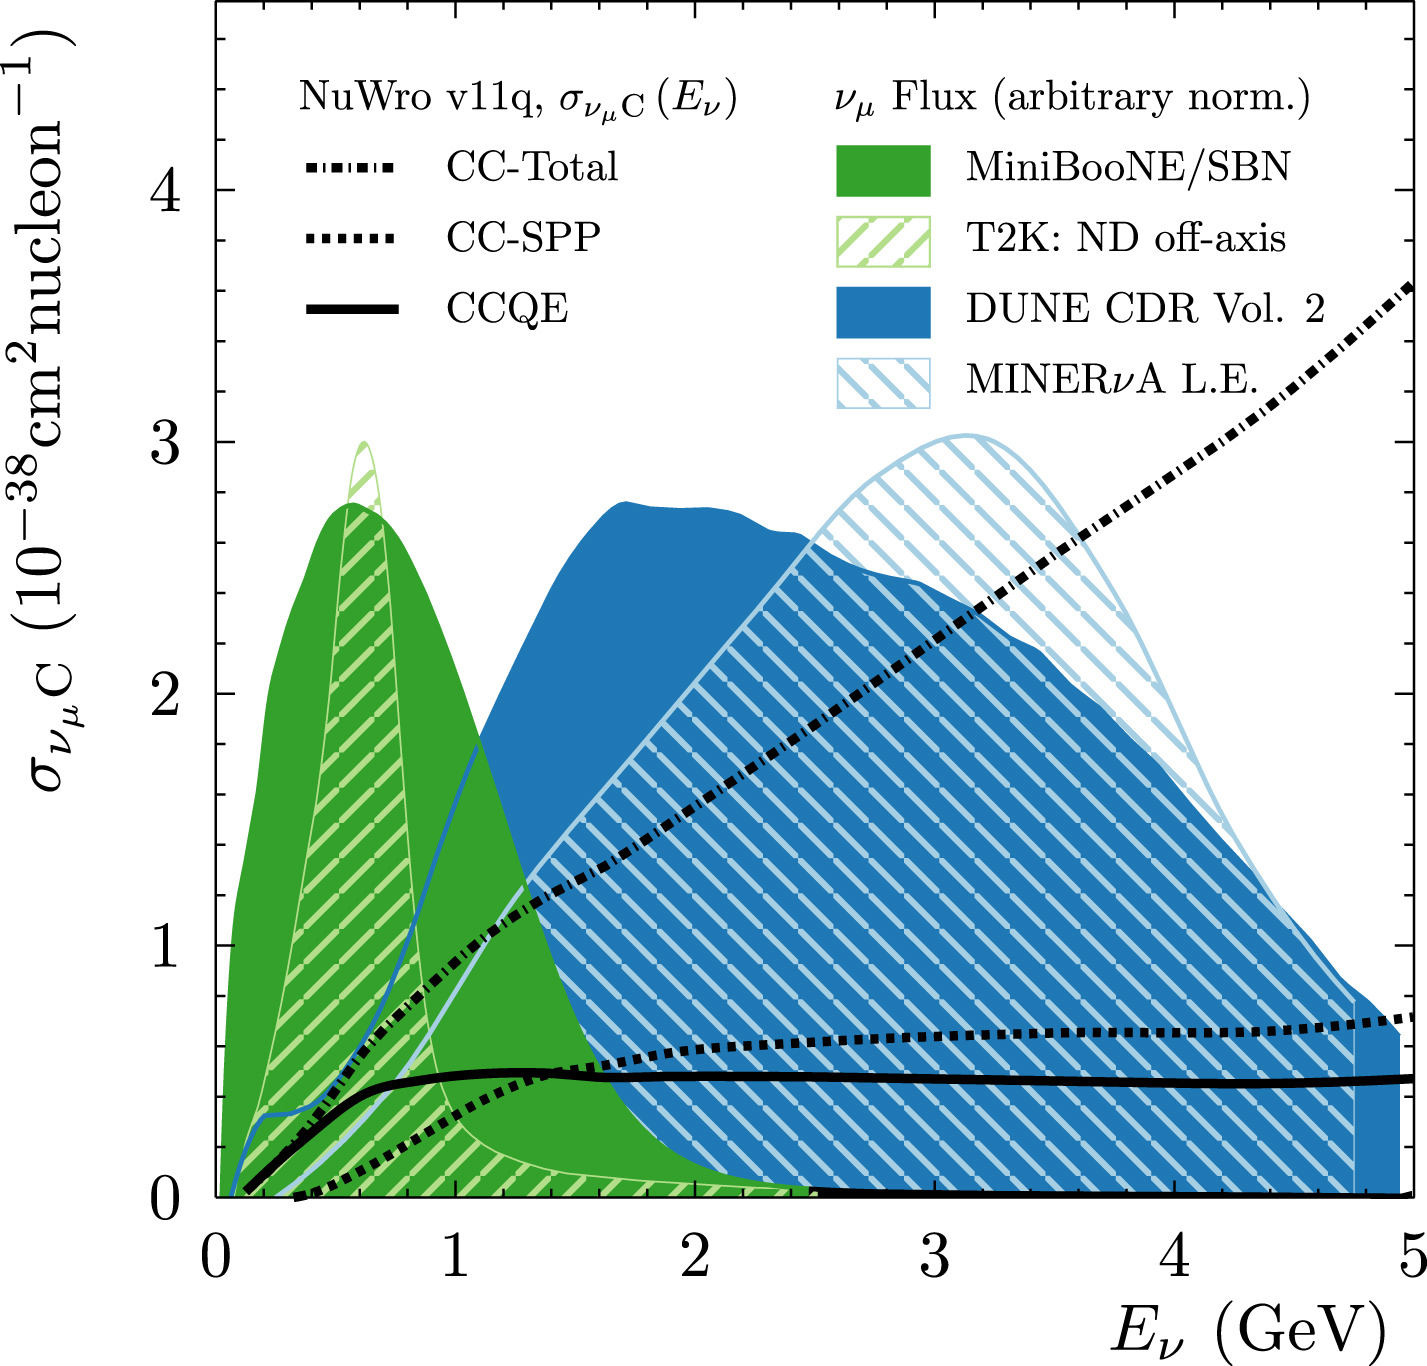
\includegraphics[width=0.5\textwidth]{cross_sections.jpg}
  \caption[Neutrino cross sections and the neutrino flux of current and future accelerator experiments.]{Figure from Ref.~\cite{Betancourt:2018bpu} showing the NuWro prediction for $\nu_\mu-^{12}C$ cross section per nucleon for {CCQE} scattering, CC single pion production (CC-SPP, dominated by {RES} diagrams), and for total CC scattering (including {DIS}). Overlaid are some of the neutrino fluxes of MINER$\nu$A, MiniBooNE, SBN, T2K off-axis and a projection for DUNE. \label{fig:compare_cross_sections}}
\end{figure}
%
The importance of nuclear effects is perhaps most famously illustrated by the measurement of the CC quasi-elastic (CCQE) process by the MiniBooNE~\cite{AguilarArevalo:2010zc} experiment. MiniBooNE is an accelerator experiment where a neutrino flux with an average energy of $\langle E_\nu \rangle \approx 800 $ MeV is directed towards a detector filled with mineral oil, made mostly of $CH$ molecules. A disagreement of $20\%$ was observed between the MC prediction and the data, unless the axial mass $M_A$ was set to be $\approx1.32$ GeV, much larger than the world-average of $M_A = 1.03 \pm 0.02$ GeV. This was later understood as a missing contribution from two-particle two-hole meson exchange currents (where the neutrino interacts with a nucleon pair, rather than with an individual nucleon), shown to be as large as $30\%$ of the CCQE cross section used by the experiment~\cite{Nieves:2011yp}.

The most common interactions of neutrino with the nucleons in the detector are displayed in \reffig{fig:interactions_diagram}. Below $\lesssim1$ GeV, CCQE scattering is most common, but at larger energies the resonant (RES) contributions start to become more important. The decay of the intermediate resonance is also affected by the nuclear medium and this has to be implemented in a nuclear-model-dependent way, such as in the so called microscopical models. Another approach is that of macroscopic models, where one makes use of the partially conserved axial current (PCAC) to relate the neutrino cross sections with the meson-nucleus cross section~\footnote{In short, PCAC is the result of the spontaneous breaking of the chiral symmetry $SU(2)_L \times SU(2)_R$ in the quark sector. Because this symmetry is explicitly broken by quark masses, the pion is massive (although quite light compared to the $\eta$ meson, for instance) and therefore the pseudo-Golstone boson of the theory.}. The PCAC relation for neutrino scattering holds only for the $q^2 = (k_1 - k_2)^2 \to 0$ limit, where the incoming neutrino momenta $k_1$ is parallel to the outgoing lepton momenta $k_2$. This is a good approximation of the cross section at large energies, but breaks down at low energies, where it is very often used~\cite{Hernandez:2009vm}. For larger neutrino energies $E_\nu\gtrsim 3$ GeV, the deep-inelastic scattering (DIS) regime start to dominate. Here, the cross section calculations are much more reliable, although nuclear effects are still in place (see Ref.~\cite{}, for instance). Past neutrino scattering experiments such as NuTeV, CCFR and CHARM operated at neutrino energies in the tens and hundreds of GeV, and provided the most precise measurements of the neutrino DIS cross sections to date. All the processes we just discussed are now  implemented in several neutrino event generators, the most popular being GENIE~\cite{Andreopoulos:2009rq}, GiBUU~\cite{Buss:2011mx}, NEUT~\cite{Hayato:2002sd} and NuWro~\cite{Juszczak:2005zs}. Different neutrino-nucleus cross section models are implemented in these generators, but one typically relies on tuning to pre-existing data to make predictions. For illustration, in \reffig{fig:compare_cross_sections} we show the NuWro predictions for CC cross sections, overlaid on neutrino fluxes in current and future accelerator experiments.







\chapter{Neutrino Scattering}
%%%%%%%%%%%%%%%%%%%%%%%%%%%%%%%%%%%%%%%%%%%%%%%%%%%%
\graphicspath{{}{tridentSM/figs/}{tridentSM/}{Diagrams/}}

This chapter is dedicated to the study of rare neutrino scattering processes. Before we can explore the possibilities to constrain new physics, it is very important we understand our theoretical predictions in the SM. In this thesis we will see that leptonic and semi-leptonic neutrino scattering is a crucial tool to understanda and go beyond the SM. This chapter is dedicated to a refresher on neutrino-electron scattering and to original work developed on the calculation and phenomenology of neutrino trident scattering. These two processes were the object of study of experiments back in the 80's and 90's, but the high beam luminosity achieved at current neutrino experiments and expected at future facilitites (typically beyond $10^{21}$ protons on target), the relatively large fiducial masses of high-$Z$ materials (typically 100~ton) of modern detectors, and improved particle idenditification (PID) capabilities allows to return to this topic at lower energies ($E_\nu =$ few~GeV) with a refreshed approach.

\section{Neutrino-electron scattering}

Neutrino-electron scattering has long been a valuable probe of both the SM and potential new physics \cite{Marciano:2003eq,deGouvea:2006hfo,PhysRevD.93.093019,Lindner:2018kjo}. It is important to note that in the presence of novel leptophilic currents, experiments searching for $e^+e^-$ tridents would also observe anomalous $\nu-e$ event rates. In fact, given the larger statistics present in the $\nu-e$ scattering sample, this channel is expected to provide the leading constraints in our scenarios with tree-level couplings to electrons. 

In order to compute the $\nu-e$ cross section in the presence of the new leptophilic interactions we need to consider an analogous modification of the NC scattering amplitude
% neutrino-electron scattering amplitude in the presence of new physics. This is a purely leptonic amplitude and can be written as
\begin{align}
    \mathcal{M}_{\rm \nu_\alpha-e} = - \frac{G_F}{\sqrt{2}}  & \left[\bar{u}(k_2)\gamma^\mu(1-\gamma_5)u(k_1)\right] \nonumber\\ & \times \left[\bar{u}(p_2)\gamma_\mu(C^{\rm V}_\alpha-C^{\rm A}_\alpha\gamma_5)u(p_1)\right],
\end{align}
where the vector ($C_V$) and axial ($C_A$) effective couplings include both the SM and BSM contributions
%
\begin{subequations}
\begin{align}
%
C^{\rm V}_\alpha &= -\frac{1}{2}+2s^2_{\rm W} + \delta_{\alpha e} + \frac{Q^{\rm V}_{e} Q^{\rm L}_{\alpha} }{2\sqrt{2}G_F} \frac{(g^\prime)^2}{M_{Z^\prime}^2+2m_eT_e},\\
%
C^{\rm A}_\alpha &= -\frac{1}{2} + \delta_{\alpha e} + \frac{Q^{\rm A}_{e} Q^{\rm L}_{\alpha} }{2\sqrt{2} G_F} \frac{(g^\prime)^2}{ M_{Z^\prime}^2 + 2m_e T_e},
\label{eq:c_prescription_nue}
%
\end{align}
\end{subequations}
with, as usual, $s_{\rm W}\equiv\sin\theta_{\rm W}$, being $\theta_{\rm W}$ the weak angle and $T_e$ is the kinetic energy of the recoil electron. The loop-induced kinetic mixing in the $L_\mu-L_\tau$ model also induces a $\nu - e$ coupling
%
\begin{equation}
C^{\rm V}_\alpha = -\frac{1}{2}+2s^2_{\rm W} + \delta_{\alpha e} + \frac{1 }{\sqrt{2}G_F} \frac{g^\prime \, e\, \varepsilon(q^2)}{M_{Z^\prime}^2+2m_eT_e}.
\end{equation}
%
The differential cross section is then given by 
%
\begin{align}\label{nuexsection}
  \frac{d\sigma_{\nu_{\alpha}-e}}{dT_e} = \frac{2m_eG_F^2}{\pi} \Bigg[ \left(C^{\rm L}_\alpha\right)^2 &+\left(C^{\rm R}_\alpha\right)^2\left(1-\frac{T_e}{E_\nu}\right)^2\nonumber\\&-C^{\rm L}_\alpha C^{\rm R}_\alpha \, m_e \frac{T_e}{E_\nu^2} \Bigg].
\end{align}
%
where the left and right handed constants are given by
%
\begin{align*}
%
C^{\rm L}_\alpha \equiv \frac{1}{2}\left(C^{\rm V}_\alpha + C^{\rm A}_\alpha\right) \qquad\text{and}\qquad
%
C^{\rm R}_\alpha \equiv \frac{1}{2}\left(C^{\rm V}_\alpha - C^{\rm A}_\alpha\right).
%
\end{align*}
%
For antineutrino scattering one obtains the cross section by exchanging $C_{\alpha}^{\rm L} \leftrightarrow C_{\alpha}^{\rm R}$. 

\subsection{Kinematics} The kinetic energy of the outgoing electron is bounded by kinematics and the energy resolution of the detector, which effectively sets a threshold energy $T_{\rm th}$ such that
%
\begin{align}
  T_{\rm th}  \le T_e \le T_{\rm max},
\end{align}
%   
with $T_{\rm max} = 2E_\nu^2/m_e+2E_\nu$, the maximum kinetic energy attainable. We define the effective total cross section for an initial neutrino energy $E_\nu$ as
%
\begin{equation}\label{eq:effective_nue_xsec}
\sigma_\text{eff}(E_\nu,T_\text{th}) = \int_{T_\text{th}}^{T_{\rm max}} \frac{d\sigma}{dT_e}\,dT_e.
\end{equation}
%
This definition also ensures that the enhancement due to very light mediators becomes constant at around $\sqrt{2 m_e T_\text{th}}$, as discussed in \refref{Lindner:2018kjo}. This is a consequence of the detector threshold and of the 2-body kinematics of the process. Finally, electroweak radiative corrections have been computed in the SM \cite{Bahcall:1995mm,Passera:2000ug}, but 
will not be included here. Since they correspond to a change of a few percent we do not expect them to affect very much our results.


\subsection{Measurements}

MINERvA

CHARM-II, CHARM, 

TEXONO, GEMMA, DAYA BAY?

Solar neutrinos - BOREXINO, SNO, Super-K

\section{Neutrino trident scattering}

Trident events are processes predicted by the SM as the result of (anti)neutrino-nucleus scattering with the production of a charged lepton pair \cite{Czyz:1964zz,Lovseth:1971vv,Fujikawa:1971nx,Brown:1971qr,Koike:1971tu}, $\pbar{\nu}_{\alpha}+{\cal{H}} \to \pbar{\nu}_{\alpha \,{\rm{or}} \, \kappa(\beta)} + \ell_{\beta}^- + \ell_\kappa^+ +{\cal{H}}$, $\{\alpha,\beta,\kappa\}\in \{e,\mu,\tau\}$\footnote{Throughout the manuscript we will consider ${\alpha,\beta, \kappa}$ as flavour indexes.} where $\cal{H}$ denotes a hadronic target. Depending on the (anti)neutrino and charged lepton flavours in the final-state, the process will be mediated by the $Z^0$ boson, $W$ boson or both. Coherent interactions between (anti)neutrinos and the atomic nuclei are expected to dominate these processes as long as the momentum transferred $Q$ is significantly smaller than the inverse of the nuclear size \cite{Czyz:1964zz}. For larger momentum transfers incoherent elastic and deep-inelastic scattering become increasingly relevant \cite{Magill:2016hgc}.
%
Although this process exists for all combinations of same-flavour or mixed flavour charged-lepton final-states, to this day only the $\nu_\mu$-induced dimuon mode, $\pbar{\nu}_\mu + {\cal{H}} \to \pbar{\nu}_\mu  + \mu^+ + \mu^- + {\cal{H}}$, has been observed. The first measurement of this trident signal performed by CHARM II~\cite{Geiregat:1990gz} is also the one with the largest statistics: 55 signal events in a beam of neutrinos and antineutrinos with $\langle E_\nu \rangle \approx 20$ GeV. Other measurements by CCFR~\cite{Mishra:1991bv} and NuTeV~\cite{Adams:1998yf} at larger energies soon followed.

As the measurement of trident events may provide a sensitive test of the weak sector~\cite{Brown:1973ih} as well as placing constraints on physics beyond the SM~\cite{Mishra:1991bv,Gaidaenko:2000hg,Altmannshofer:2014pba,Kaneta:2016uyt,Ge2017,Magill:2017mps,Falkowski:2018dmy} it is relevant to investigate how to probe it further at current and future neutrino experiments. Atmospheric neutrinos, for instance, may provide a feasible measurement of the dimuon channel, as pointed out in \refref{Ge2017}\footnote{The authors of \refref{Ge2017} have performed the full calculation of the trident process and made their code publicly available.}. Other trident modes were also re\-cog\-ni\-zed to be relevant by the authors of Ref.~\cite{Magill:2016hgc} who calculated the cross sections for trident production in all possible flavour combinations and estimated the number of events expected for the DUNE and SHiP experiments. They used the Equivalent Photon Approximation (EPA)~\cite{Belusevic:1987cw} to compute the cross section in the coherent and incoherent regimes of the scattering. The EPA, however, is known to breakdown for final state electrons~\cite{Kozhushner:1962aa, Shabalin:1963aa, Czyz:1964zz} leading, as we will demonstrate here, to an overestimation of the cross section that in some cases is by more than 200\%. 

In this work, we present a unified treatment of the coherent and incoherent trident calculation beyond the EPA for all modes. We then compute the number and distribution of events expected in each mode at various near detectors, devoting particular attention to the case of liquid argon (LAr) detectors, as they are expected to lead the field of precision neutrino scattering measurements over the next few decades thanks to their excellent tracking and calorimetry capabilities. Finally, we address the likely backgrounds that may hinder these experimental searches --- a question that we believe to be of utmost importance given the rarity of the process, and one that has been omitted in earlier sensitivity studies \cite{Magill:2016hgc,Altmannshofer:2014pba}. 

This paper is organized as follows. In Sec.~\ref{sec:xsec}, we explain how to correctly calculate the trident SM cross sections, comparing our results to the EPA and explicitly showing the breakdown of this approximation. In Sec.~\ref{sec:LAr}, we discuss the trident event rates and kinematic distributions at the near detectors of several present and future neutrino oscillation experiments based on LAr technology: the three detectors of the Short-Baseline Neutrino (SBN) Program at Fermilab~\cite{SBNproposal} and the near detector for the long-baseline Deep Underground Neutrino Experiment (DUNE)~\cite{Acciarri:2016ooe,DUNECDRvolII}, also located at Fermilab. We also consider the potential gains from an optimistic future facility: a 100 t LAr detector subject to the novel low-systematics neutrino beam of the Neutrinos from STORed Muons ($\nu$STORM) project~\cite{Soler:2015ada,nuSTORM2017}. 
%
We discuss the sources of background events at these facilities, providing a GENIE-level analysis \cite{Andreopoulos2009} of how to reduce these backgrounds and assessing the impact they are expected to have on the trident measurement. 
%
In Sec.~\ref{sec:others}, we discuss other near detectors that use more conventional technologies: the Interactive Neutrino GRID (INGRID)~\cite{Abe:2011xv,Abe:2015biq,Abe:2016fic,Abe:2016tez}, the on-axis iron near detector for T2K at J-PARC, as well as three detectors at the Neutrino at the Main Injector (NuMI) beamline at Fermilab, the one for the Main INjector ExpeRiment $\nu$-A (MINER$\nu$A)~\cite{Altinok:2017xua,MINERvA:2017} and the near detectors for the Main Injector Oscillation Search (MINOS)~\cite{Adamson:2014pgc,AlpernBoehm} and the Numi Off-axis $\nu_e$ Appearance (NO$\nu$A) experiment~\cite{Wang:Biao,sanchez_mayly_2018_1286758}. 
%

%%%%%%%%%%%%%%%%%%%%%%%%%%%%%%%%%%%%%%%%%%%%%%%%%%%%
\section{Trident Production Cross Section}\label{sec:xsec}

In this section we consider neutrino trident production in the SM, defined as the process where a (anti)neutrino scattering off a hadronic system ${\cal H}$ produces a pair of same-flavour or mixed flavour charged leptons 
%
\begin{equation}
\pbar{\nu}_{\alpha}(k_1) \,+\, {\cal H}(P) \,\to\, \pbar{\nu}_{\alpha^\prime} (k_2) \,+\, \ell_\beta^- (p_-)  \,+\, \ell_\kappa^+ (p_+) \,+\, {\cal H}(P^\prime),
\label{eq:indices}
\end{equation}
%
where $\beta (\kappa)$ corresponds to the flavour index of the negative (positive) charged lepton in both neutrino and antineutrino cases. 
%
Neutrino trident scattering can be divided into three regimes depending on the nature of the hadronic target: coherent, incoherent elastic and deep inelastic, when the neutrino scatters off the nuclei, nucleons and quarks, respectively. At the energies relevant for neutrino oscillation experiments, the deep inelastic scattering contribution amounts at most to 1\% of the total trident production cross section \cite{Magill:2016hgc} and we will not consider it further.

The cross section for trident production has been calculated before in the literature, both in the context of the $V-A$ theory~\cite{Czyz:1964zz,Lovseth:1971vv,Fujikawa:1971nx} and in the SM~\cite{Brown:1973ih}, while the EPA treatment was developed in Refs.~\cite{Kozhushner:1962aa,Shabalin:1963aa,Belusevic:1987cw}. Most calculations have focused on the coherent channels \cite{Czyz:1964zz,Lovseth:1971vv,Fujikawa:1971nx,Brown:1973ih,Belusevic:1987cw} but the incoherent process has been considered in \cite{Czyz:1964zz,Lovseth:1971vv}. More recently, calculations using the EPA have been performed for coherent scattering with a dimuon final-state \cite{Altmannshofer:2014pba}, and for all combinations of hadronic targets and flavours of final-states in \cite{Magill:2016hgc}. While the EPA is expected to agree reasonably well with the full calculation for coherent channels with dimuon final-states, the assumptions of this approximation are invalid for the coherent process with electrons in the final-state \cite{Kozhushner:1962aa,Shabalin:1963aa,Czyz:1964zz}. 
%
For this reason, we perform the full $2\to 4$ calculation without the EPA in a manner applicable to any hadronic target, following a similar approach to Refs.~\cite{Czyz:1964zz,Lovseth:1971vv}. Our treatment of the cross section allows us to quantitatively assess the breakdown of the EPA in both coherent and incoherent channels for all final-state flavours, an issue we come back to in Sec.~\ref{sec:EPAbreakdown}.

We write the total cross section for neutrino trident production off a nucleus ${\cal N}$ with $Z$ protons and $(A-Z)$ neutrons as the sum
%
\begin{equation}
\sigma_\mathrm{\nu {\cal N}} = \sigma_\mathrm{\nu c} +\sigma_\mathrm{\nu d}\, ,
\end{equation}
where $\sigma_\mathrm{\nu c}$ ($\sigma_\mathrm{\nu d}$) is the coherent (incoherent) part of the cross section. 
%
%%%%%%%%%%%% SM DIAGRAMS %%%%%%%%%%%%%%%%
\unitlength = 0.9mm
\begin{figure}[t]
% \centering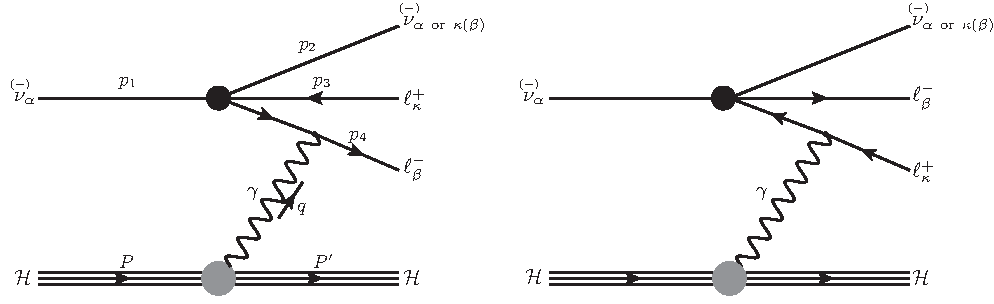
\includegraphics[width=\textwidth]{tridentSM/figs/SM-trident.pdf}
\centering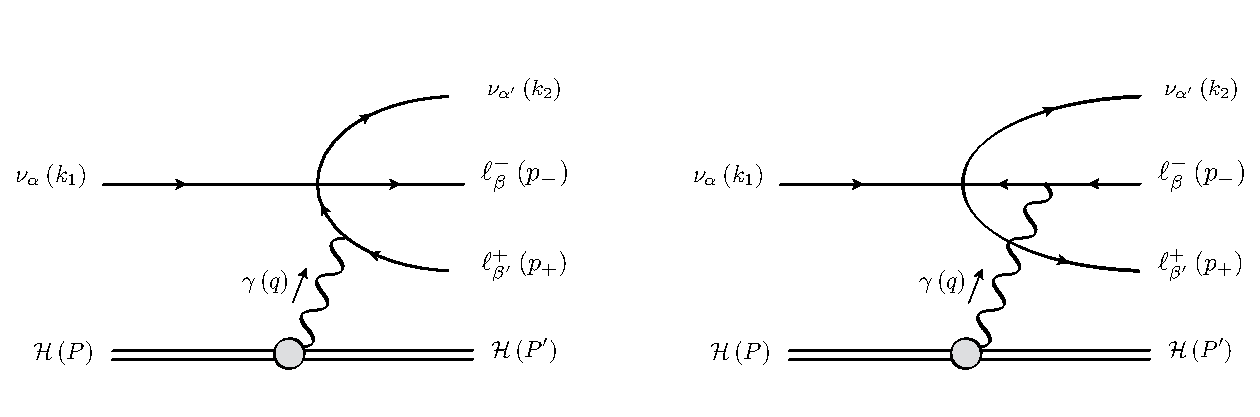
\includegraphics[width=\textwidth]{Neutrino_trident_production.pdf}
\caption[Neutrino trident production with a contact approximation.]{Diagrams contributing to the neutrino trident process in the four-point interaction limit of the Standard Model.  
\label{fig:Tdiagrams}}
\end{figure}

%%%%%%%%%%%%%%%%%%%%%%%%%%%%%%%%%%%%%%%%%
%
The relevant diagrams for these processes in the coherent or incoherent 
regimes involve the boson $Z^0$, $W$ or both mediators, depending on the particular mode. In the four-point interaction limit, depicted in \reffig{fig:Tdiagrams}, these reduce to only two contributions\footnote{An additional diagram involving a $WW\gamma$ vertex has also been neglected, since it is of order $1/M_W^4$.}, one where the photon couples to the negatively and one to the positively charged lepton. 
In Table \ref{tab:tridentmodes}, we present the processes we will consider in this thesis as well as the SM contributions present in each. Although our formalism applies also to processes with final-state $\tau$ leptons, the increased threshold and their suppressed cross section makes them irrelevant for the experiments of interest in this study and we do not consider them further.
%
The trident amplitude for a coherent (${\rm X=c}$) or incoherent (${\rm X=d}$) scattering regime can be written as
%
\begin{equation}
i \mathcal{M} = \mathrm{L}^\mu (\{p_i\},q) \, \frac{-ig_{\mu \nu}}{q^2} \, \mathrm{H}_{\rm X}^{\nu}(P,P^{\prime})\, ,
\end{equation}
%
where $\{p_i\}=\{k_2,p_-,p_+\}$ is the set of outgoing leptonic momenta. $ \mathrm{L}^\mu (\{p_i\},q)$ is the total leptonic amplitude 
%
\begin{align}
\mathrm{L}^\mu & \equiv - \frac{ie G_F}{\sqrt{2}}[\bar{u}(k_2)\gamma^\tau(1-\gamma_5)u(k_1)] \times 
\bar{u}(p_-)\left[\gamma_\tau(V-A\gamma_5)\frac{1}{(\slashed{q}-\slashed{p}_+ - m_+)}\gamma^\mu \right . \nonumber \\ 
& \left . + \gamma^\mu \frac{1}{(\slashed{p}_- -\slashed{q}-m_-)} \gamma_\tau (V-A \gamma_5) \right] v(p_+)\, ,
\label{eq:Lmu}
\end{align}
%
and $\mathrm{H}_{\rm X}^{\nu}(P,P^{\prime})$ is the total hadronic amplitude
\begin{align}
H_{\rm X}^\nu  &\equiv \langle {\cal H}(P) \vert J_\mathrm{E.M.}^\nu (q^2)\vert {\cal H}(P^\prime)\rangle\, ,
\label{eq:Hmu}
\end{align}
%
with  $q \equiv P - P^\prime$ denoting the transferred momentum, $m_+$ ($m_-$) the positively (negatively) charged lepton mass and ${J}^\nu_{\rm{E.M.}} (q^2)$ the electromagnetic current for the hadronic system ${\cal H}$ (a nucleus or a nucleon). The flavour indices have been ommitted from the vector $V$ and axial $A$ couplings, determined by $V \equiv g_{V}^{\alpha^\prime} \delta_{\alpha\alpha^\prime}\delta_{\beta\beta^\prime}+\delta_{\alpha^\prime \beta^\prime}\delta_{\alpha\beta}$ and $A \equiv g_{A}^{\alpha^\prime} \delta_{\alpha\alpha^\prime}\delta_{\beta\beta^\prime}+\delta_{\alpha^\prime \beta^\prime}\delta_{\alpha\beta}$ in accordance to~\refeq{eq:indices} and shown in~\reftab{tab:tridentmodes}.
%
\begin{table}[t]
\begin{center}
\begin{tabular}{cccc}
\hline
Trident channel &  SM Contributions & V & A \\
\hline
${\nu}_\mu\, {\cal H} \to {\nu}_\mu\, \mu^- \mu^+\,  {\cal H}$  & CC + NC &$\sfrac{1}{2} + 2 \,\sw^2$&$\sfrac{1}{2}$\\
${\nu}_\mu\, {\cal H} \to {\nu}_\mu\,  e^- e^+\, {\cal H}$ & NC&$-\sfrac{1}{2} + 2 \,\sw^2$&$-\sfrac{1}{2}$\\
${\nu}_\mu\, {\cal H} \to {\nu}_e\,  e^+ \mu^-\, {\cal H}$  & CC&$1$&$1$\vspace{2ex}\\
${\nu}_e\, {\cal H} \to {\nu}_e\,  e^- e^+\, {\cal H}$ &  CC + NC &$\sfrac{1}{2} + 2 \,\sw^2$&$\sfrac{1}{2}$\\
${\nu}_e\, {\cal H} \to {\nu}_e\,  \mu^- \mu^+\, {\cal H}$ & NC &$-\sfrac{1}{2} + 2 \,\sw^2$&$-\sfrac{1}{2}$\\
${\nu}_e\, {\cal H} \to {\nu}_\mu\,  \mu^+ e^-\, {\cal H}$ & CC &$1$&$1$\\

\hline
\end{tabular}
\end{center}
\caption[Neutrino trident production channels and their SM contributions.]{\label{tab:tridentmodes} Neutrino trident processes considered in this thesis. Antineutrino induced channels are analogous.}
\end{table}
%

We can write the differential cross section as
\begin{align}
\frac{\dd^2 \sigma_{\nu  {\rm X}}}{\dd Q^2 \dd \hat{s}}= \frac{1}{32  \pi^2(s-M_{\cal H}^2)^2}\frac{\mathrm{H}_{\rm X}^{\mu\nu}\mathrm{L}_{\mu\nu}}{Q^4}\, ,
\end{align}
where $s = (k_1 + P)^2$, $\hat{s} \equiv 2\,(k_1 \vdot q)$, $Q^2 = -q^2$ and $M_{\cal H}$ is the mass of the hadronic target. We have also introduced the hadronic tensor $\mathrm{H}_{\rm X}^{\mu \nu}$
%
\begin{align}
\mathrm{H}_{\rm X}^{\mu\nu} &\equiv \overline{\sum_{\rm{spins}}}  \left(\mathrm{H}_{\rm X}^\mu\right)^* \mathrm{H}_{\rm X}^\nu.
%
\end{align}
The two scattering regimes in which the hadronic tensor is computed will be discussed in more detail in Sec.~\ref{sec:had}. The leptonic tensor, $\mathrm{L}^{\mu \nu}$, integrated over the phase space of the three final-state leptons, $\dd^{3} \Pi \left(k_1 + q; \{p_i\}\right)$, and merely summed over final and initial spins is given by
%
\begin{equation}
\mathrm{L}^{\mu \nu} (k_1, q) \equiv  \int \dd ^{3} \Pi \left(k_1 + q; \{p_i\}\right) \left( \sum_{\rm{spins}} \left(  \mathrm{L}^\mu \right)^*  \mathrm{L}^\nu  \right)\, .
\label{eq:Lmunu}
\end{equation}
We can use $\mathrm{L}^{\mu \nu}$ to define two scalar functions, one related to the longitudinal ($\mathrm{L}_{\mathrm{L}}$) and the other to the transverse ($\mathrm{L}_{\mathrm{T}}$) polarization of the exchanged photon
\begin{equation}
\mathrm{L}_{\mathrm{T}} = -\frac{1}{2}\left( g^{\mu \nu} - \frac{4Q^2}{\hat{s}^2} k_1^\mu k_1^\nu \right) \mathrm{L}_{\mu \nu}, \quad \mathrm{and} \quad \mathrm{L_{L}} =  \frac{4Q^2}{\hat{s}^2} k_1^\mu k_1^\nu \mathrm{L}_{\mu \nu}\, .\label{eq:LT_LL}
\end{equation}
%
This allows us to write the differential cross section as a sum of a longitudinal and a transverse contribution \cite{Hand:1963bb} as follows
%
\begin{align}
\frac{\dd^2 \sigma_{\nu  {\rm X}}}{\dd Q^2 \dd \hat{s}} &= \frac{1}{32 \pi^2} \frac{1}{\hat{s}\,Q^2} \left [ h_{\rm X}^\mathrm{T}(Q^2, \hat{s}) \, \sigma^\mathrm{T}_{\nu \gamma} (Q^2, \hat{s}) + h_{\rm X}^\mathrm{L}(Q^2, \hat{s}) \, \sigma^\mathrm{L}_{\nu \gamma} (Q^2, \hat{s}) \right] \, ,\label{eq:full_diff_xsec}
\end{align}
%
where we have defined two functions for the flux of longitudinal and transverse virtual photons 
%
\begin{subequations}
\label{eq:splitting_function}
\begin{align}
%
h_{\rm X}^\mathrm{T}(Q^2, \hat{s})  &\equiv \frac{2}{(E_\nu M_{\cal H})^2} \left[ k_{1 \mu} k_{1\nu} -\frac{\hat{s}^2}{4 Q^2} \, g_{\mu \nu} \right]\mathrm{H}_{\rm X}^{\mu \nu} , \quad \text{and} \\ \quad
h_{\rm X}^\mathrm{L}(Q^2, \hat{s})  &\equiv \frac{1}{(E_\nu M_{\cal H})^2} \, k_{1\mu} k_{1\nu}\, \mathrm{H}_{\rm X}^{\mu \nu}\, ,
%
\end{align}
%
\end{subequations}
%
and two leptonic neutrino-photon cross sections associated with them\footnote{Note that we include a factor of $1/2$ in $\sigma^\mathrm{T}_{\nu \gamma}$ to match the polarization averaging of the on-shell cross section: $\sigma_{\nu \gamma}^{\rm on-shell} = \frac{1}{2 \hat{s}} \left( \overline{\sum}_r (\epsilon_r^\mu)^* \epsilon^\nu_r \, {\rm L}_{\mu\nu} \right) \big\vert_{Q^2=0} = \frac{1}{4 \hat{s}} \left( - g^{\mu\nu} L_{\mu\nu}\right) \big\vert_{Q^2=0} = \frac{{\rm L_T}}{2 \hat{s}}\big\vert_{Q^2=0} = \sigma_{\nu\gamma}^\text{T}(0,\hat{s})$.}
%
\begin{equation}
\sigma^\mathrm{T}_{\nu \gamma} (Q^2, \hat{s})  = \frac{\mathrm{L_T}}{2 \hat{s}}\, , \quad \mathrm{and} \quad
\sigma^\mathrm{L}_{\nu \gamma} (Q^2, \hat{s})  = \frac{\mathrm{L_L}}{\hat{s}}\, .
\end{equation}
%
The kinematically allowed region in the $(Q^2,\hat{s})$ plane can be obtained by considering the full four-body phase space, as in~\cite{Czyz:1964zz,Lovseth:1971vv,Fujikawa:1971nx}. The limits for such physical region are given by
\begin{subequations}\label{eq:qslimts}
	\begin{align}
		Q_{\rm min}^2&=\frac{M_{\cal H} \hat{s}^2}{2E_\nu(2E_\nu M_{\cal H}-\hat{s})},&\  
        Q_{\rm max}^2&=\hat{s}-m_L^2,\label{eq:qlimts}\\
        \hat{s}_{\rm min}&=\frac{E_\nu}{2E_\nu + M_{\cal H}}\left[m_L^2+2E_\nu M_{\cal H} -\Delta\right]&\  
        \hat{s}_{\rm max}&=\frac{E_\nu}{2E_\nu + M_{\cal H}}\left[m_L^2+2E_\nu M_{\cal H} +\Delta\right],\label{eq:shatlimts}
	\end{align}
\end{subequations}
%
with $m_L\equiv m_++m_-$, and
%
\begin{align*}
	\Delta \equiv \sqrt{(2E_\nu M_{\cal H}-m_L^2)^2-4M_{\cal H}^2 m_L^2}\,.
\end{align*}
%
Let us emphasize that \refeq{eq:full_diff_xsec} is an exact decomposition, and does not rely on any approximation of the process. In the following section, we will show how to calculate the flux functions $h_{\rm X}^\mathrm{T}$ and $h_{\rm X}^\mathrm{L}$ from Eq.~\ref{eq:splitting_function} in different scattering regimes. The total cross section for the process can then be computed by finding $\sigma^\mathrm{L}_{\nu \gamma}$ and $\sigma^\mathrm{T}_{\nu \gamma}$ from Eqs.~(\ref{eq:Lmu}), (\ref{eq:Lmunu}) and (\ref{eq:LT_LL}) and integrating over all allowed values of $Q^2$ and $\hat{s}$. Note that $\sigma^\mathrm{L}_{\nu \gamma}$ and $\sigma^\mathrm{T}_{\nu \gamma}$ are universal functions for a given leptonic process and need only to be computed once.

%%%%%%%%%%%%%%%%%%%%%%%%%%%%%%%%%%%%%%%%%%%%%%%%%%%%%%%%%%%%%%
\subsection{Hadronic Scattering Regimes}\label{sec:had}

Depending on the magnitude of the virtuality of the photon, $Q = \sqrt{-q^2}$, the hadronic current can contribute in different ways to the trident process. Thus, given the decomposition in \refeq{eq:full_diff_xsec}, the change in the hadronic treatment translates to computing the flux factors $h_{\rm X}^\mathrm{T}$ and $h_{\rm X}^\mathrm{L}$ for each scattering regime.  From those flux factors, $\sigma_{\nu\mathrm{c}}$ and $\sigma_{\nu\mathrm{d}}$ can be calculated.

%%%%%%%%%%%%%%%%%%%%%%%%%%%%%%%%%%%%%%%%%%%%%%%%%%
\subsubsection{Coherent Regime (${\rm H}^{\mu \nu}_{\rm c}$)}

In the coherent scattering regime the incoming neutrino interacts with the whole nucleus without resolving its substructure. For this to occur frequently, we need small values of $Q$. Despite the relatively large neutrino energies in contemporary neutrino beams, this is still allowed for trident.

In this regime, the hadronic tensor $\mathrm{H}^{\mu\nu}_\mathrm{c}$ for a ground state spin-zero nucleus of charge $Z e$ can be written in terms 
of the nuclear electromagnetic form factor $F(Q^2)$, discussed in more detail in Appendix~\ref{app:formfactors}, as
%
\begin{equation}
\mathrm{H}^{\mu \nu}_\mathrm{c} =  4Z^2 e^2 \left| F (Q^2)\right|^2 \left(P^\mu - \frac{q^\mu}{2}\right) \left(P^\nu - \frac{q^\nu}{2}\right).
\end{equation}
%
From Eq.~\ref{eq:splitting_function}, we find that the transverse and longitudinal flux functions for the coherent regime are
%
\begin{subequations}\label{eq:hcoh}
\begin{align}
h^\mathrm{T}_\mathrm{c}(Q^2, \hat{s})  &=  8 Z^2 e^2   \left(1 - \frac{\hat{s}}{2E_\nu M} - \frac{\hat{s}^2}{4 E_\nu^2 Q^2}\,\right) |F (Q^2)|^2\, , \\
h^\mathrm{L}_\mathrm{c}(Q^2, \hat{s})  &=  4 Z^2 e^2  \left(1 - \frac{\hat{s}}{4E_\nu M}\right)^2 |F (Q^2)|^2\, ,
\end{align}
\end{subequations}
where $E_\nu$ is the energy of the incoming neutrino and $M$ is the nuclear mass. For a fixed value of $\hat{s}$ in the physical region, the $h^{\rm T}_{\rm c}$ flux function becomes zero at $Q_{\rm min}$ while the longitudinal component does not. This different behaviour can be seen explicitly in their definitions, Eqs. \eqref{eq:hcoh}, as the terms in the parenthesis in $h^{\rm T}_{\rm c}$ cancel each other at $Q_{\rm min}$. This does not occur for $h^{\rm L}_{\rm c}$ since the physical values of $\hat{s}$ are always smaller than $E_\nu M$ in this hadronic regime. 
Due to this fact, $Q_{\rm min}$, which according to  Eq.\ \eqref{eq:qlimts} depends on  both the  neutrino energy and target material, can be approximated to
\begin{align*}
	Q_{\rm min} \approx \frac{\hat{s}}{2E_{\nu}},
\end{align*}
which only depends on the incoming neutrino energy. On the other hand, as $Q$ becomes large, the flux functions $h^{T,L}$ become quite similar, $h^{\rm T}_{\rm c}\approx 2 h^{\rm L}_{\rm c}$, and favour small values of $\hat{s}$. After some critical value of the virtuality $Q$, $h^{\rm T, L}_{\rm c}$ become negligible due to the nuclear form factor. The $Q$ value at which this happens depends on the target material, but not on the incoming neutrino energy. For instance, in the case of an Ar target
the flux functions basically vanish for $Q\gtrsim 250$ MeV.

The final cross sections for coherent neutrino trident production on Argon can be seen in \reffig{fig:coh_xsec}. Despite thresholds being important for the behaviour of these cross sections for GeV neutrino energies, we can see that mixed channels quickly become the most important due to their CC nature. At large energies one can then rank the cross sections from largest to smallest as CC, CC+NC, and NC only channels. Nevertheless, one must be aware of the fact that the cross sections are dominated by low $Q^2$ even at large energies, leading to large effects due to the final-state lepton masses as discussed in \cite{Magill:2016hgc}.

\begin{figure}[t]
\centering
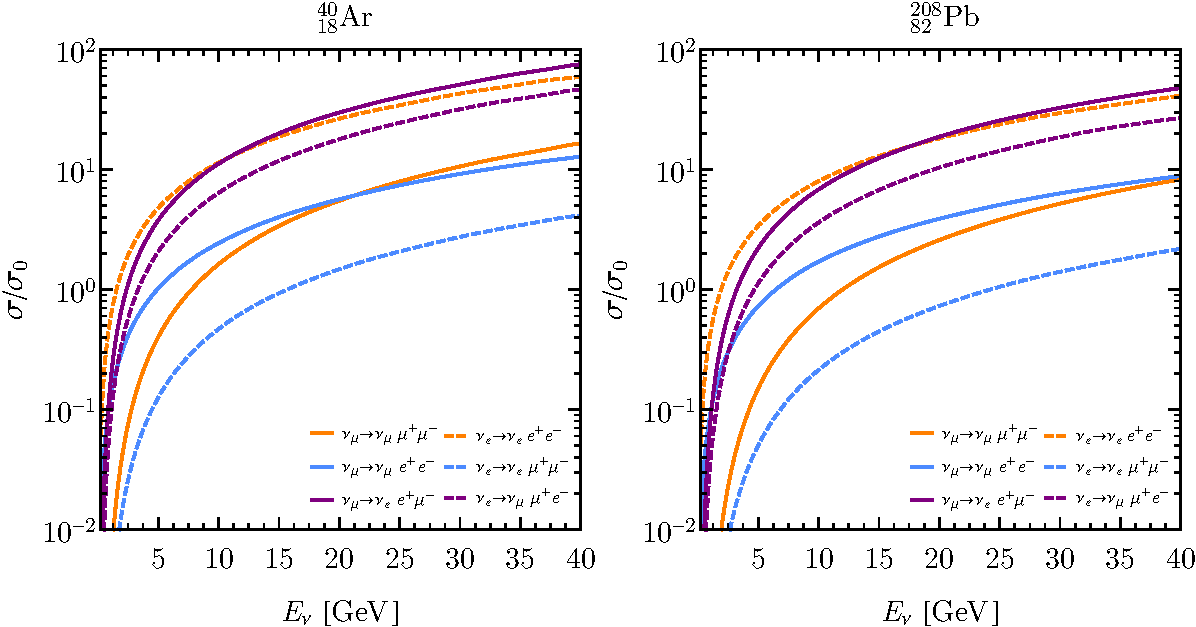
\includegraphics[width=\textwidth]{figs/Xsec_4PS_coh.pdf}
\caption[Coherent neutrino trident production total cross sections.]{Cross sections for coherent neutrino trident production on $^{40}$Ar (left) and  $^{208}$Pb (right) normalized to $\sigma_0 =  Z^2\, 10^{-44}$ cm$^2$. The full (dashed) lines correspond to the scattering of an incoming $\nu_\mu$ ($\nu_e$) produced by the NC (light-blue), CC (purple), and CC+NC (orange) SM interactions. \label{fig:coh_xsec}}
\end{figure}


%%%%%%%%%%%%%%%%%%%%%%%%%%%%%%%%%%%%%%%%%%%%%%%%%%%%
\subsubsection{Incoherent Regime ($\mathrm{H}^{\mu\nu}_\mathrm{d}$)}

At larger $Q^2$, the neutrino interacts with the individual nucleons of the nucleus. In this incoherent regime $\mathrm{H}^{\mu\nu}_\mathrm{d}$ is given by the sum of the contributions of the two types of nucleons: protons ($\mathrm{N=p}$) and neutrons ($\mathrm{N=n}$), so
\begin{equation}
\mathrm{H}^{\mu \nu}_\mathrm{d} (P, P^\prime) = Z\, \mathrm{H}^{\mu \nu}_\mathrm{p} (P, P^\prime)+
(A-Z)\,\mathrm{H}^{\mu \nu}_\mathrm{n}(P, P^\prime)\, ,
\end{equation}
where each $\mathrm{H}^{\mu \nu}_\mathrm{N}$ is the square of the matrix element of the nucleon electromagnetic current summed over final and averaged over initial spins. Neglecting second class currents, the matrix elements take the form
\begin{equation}
\bra{\mathrm{N}(P^\prime)} {J}^\mu_{\rm{E.M.}} (Q^2) \ket{\mathrm{N} (P) } = e \, \overline{u}_\mathrm{N} (P^\prime) \left[ \gamma^\mu F^\mathrm{N}_1(Q^2) - i \frac{\sigma^{\mu \nu} q_{\nu}}{2 M_{\rm N}} F^\mathrm{N}_2(Q^2) \right] u_\mathrm{N}(P)\, ,
\end{equation}
%
with $F^\mathrm{N}_{1,2}(Q^2)$ the Dirac and Pauli form factors, respectively. The hadronic tensors are then given by \cite{Kniehl:1990iv}
%
\begin{equation}
\mathrm{H}^{\mu \nu}_\mathrm{N} = e^2 \left[ 4 \, H_1^\mathrm{N}(Q^2) \left(P^\mu - \frac{q^\mu}{2}\right)\left(P^\nu - \frac{q^\nu}{2}\right) - H_2^\mathrm{N}(Q^2) \left( Q^2 g^{\mu \nu} + q^\mu q^\nu \right) \right]\, ,
\end{equation}
%
where the  $H_1^\mathrm{N}(Q^2)$ and $H_2^\mathrm{N}(Q^2)$ form factors, functions of $F^\mathrm{N}_{1,2}(Q^2)$, are given in Appendix~\ref{app:formfactors}. The flux functions in the incoherent regime can then be calculated as
\begin{subequations}\label{eq:dcoh}
\begin{align}
h^\mathrm{T}_\mathrm{N}(Q^2, \hat{s})  &=  8 \, e^2 \left[ \left(1 - \frac{\hat{s}}{2E_\nu M_{\rm N}} - \frac{\hat{s}^2}{4 E_\nu^2 Q^2 }\,\right) H_1^\mathrm{N}(Q^2) + \frac{\hat{s}^2}{8E_\nu^2 M_{\rm N}^2}  H_2^\mathrm{N}(Q^2)\right ]\, ,\label{eq:hTdiff}\\
%
h^\mathrm{L}_\mathrm{N}(Q^2, \hat{s})  &=  4 e^2 \, \left[ \left(1-\frac{\hat{s}}{4 E_\nu M_{\rm N}} \right)^2 H_1^\mathrm{N}(Q^2)  - \frac{\hat{s}^2}{16 E_\nu^2 M_{\rm N}^2} H_2^\mathrm{N}(Q^2)\right]\, .\label{eq:hLdiff}
\end{align}
\end{subequations}
%
In the case of the proton, the flux functions $h^{\rm T, L}_{\rm p}$ have some unique features given the presence of both electric and magnetic contributions. Specifically, the transverse function is non-zero at $Q=Q_{\rm min}$ for a fixed $\hat{s}$, due to the additional term proportional to $H_2^{\rm p}$. Indeed, for large values of $\hat{s}$, the $H_2^{\rm p}$ term dominates the transverse function. An opposite behaviour occurs for the longitudinal component. There, the $H_1^{\rm p}$ term dominates over the second term for all physical values of $\hat{s}$, $Q$, and for any incoming neutrino energy. On the other hand, the flux functions of the neutron, which have only 
the magnetic moment contribution, have somewhat different characteristics. While 
$h^{\rm T}_{\rm n}$ behaves similarly to $h^{\rm T}_{\rm p}$, that is, it is dominated by the second term for large values of $\hat{s}$, $h^{\rm L}_{\rm n}$ is zero at $Q_{\rm min}$ due to the exact cancellation between the $H_{1,2}^{\rm n}$ terms. This cancellation is not evident from Eq.\ ~\eqref{eq:hLdiff}; however, simplifying the longitudinal component for the neutron case, one finds
\begin{align*}
	h^\mathrm{L}_\mathrm{n}(Q^2, \hat{s})  &=4 e^2 \left(1+\frac{Q^2}{4M_{\rm n}^2}\right)\frac{Q^2}{4 M_{\rm N}^2}\left( 1 - \frac{\hat{s}}{2 E_\nu M_{\rm N}} - \frac{\hat{s}^2}{4 E_\nu^2 Q^2} \right) \left| F^\mathrm{n}_2(Q^2) \right|^2,
\end{align*}
which is zero for $Q=Q_{\rm min}$. Also, this shows why $h^{\rm L}_{\rm p}$ does not 
vanish at $Q_{\rm min}$ since there we have the additional contribution of the electric component. 

When the neutrino interacts with an individual nucleon inside the nucleus, one must be aware of the nuclear effects at play. One such effect is Pauli blocking, a suppression of neutrino-nucleon interactions due to the Pauli exclusion principle. Modelling the nucleus as an ideal Fermi gas of protons and neutrons, one can take Pauli blocking effects into account by requiring that the hit nucleon cannot be in a state which is already occupied \cite{Brown:1971qr}. This requirement is implemented in our calculations by a simple replacement of the differential incoherent cross section
\begin{align*}
\frac{\dd^2 \sigma_{\nu  \mathrm{d}}}{\dd Q^2 \dd \hat{s}}\to f (|\vec{q}|) \, \frac{\dd^2 \sigma_{\nu  \mathrm{d}}}{\dd Q^2 \dd \hat{s}},
\end{align*}
where $|\vec{q}|$ is the magnitude of the transferred three-momentum in the lab frame. In particular, following \cite{Brown:1971qr}, assuming an equal density of neutrons and protons, we have
%
\begin{equation}
f (|\vec{q}|) = \begin{cases} \displaystyle
                    \frac{3}{2} \frac{|\vec{q}|}{2 \, k_F} - \frac{1}{2} \left( \frac{|\vec{q}|}{2 \, k_F} \right)^3 ,\, &\mathrm{if }\;\; |\vec{q}| < 2\, k_F\, ,\\
                    1,\, &\mathrm{if }\;\; |\vec{q}| \geq 2 \, k_F\, ,
                \end{cases}
\end{equation}
%
where $k_F$ is the Fermi momentum of the gas, taken to be $235$ MeV. This is a rather low value of $k_F$ and the assumption of equal density of neutrons and protons must be taken with care for heavy nuclei. We refrain from trying to model any additional nuclear effects as we believe that this is the dominant effect on the total incoherent rate, particularly when requiring no hadronic activity in the event. The net result is a reduction of the incoherent cross section by about $50\%$ for protons and $20\%$ for neutrons. Unless clearly stated otherwise, we always include Pauli blocking in our calculations.

Our final cross sections for this regime can be seen in \reffig{fig:dif_xsec}. One can clearly see that the neutron contribution is subdominant, and that, up to factors of $Z^2$, the proton one is comparable to the coherent cross section. Note that now the typical values of $Q^2$ are much larger than in the coherent regime and the impact of the final-state lepton masses is much smaller. 

\begin{figure}[t]
\centering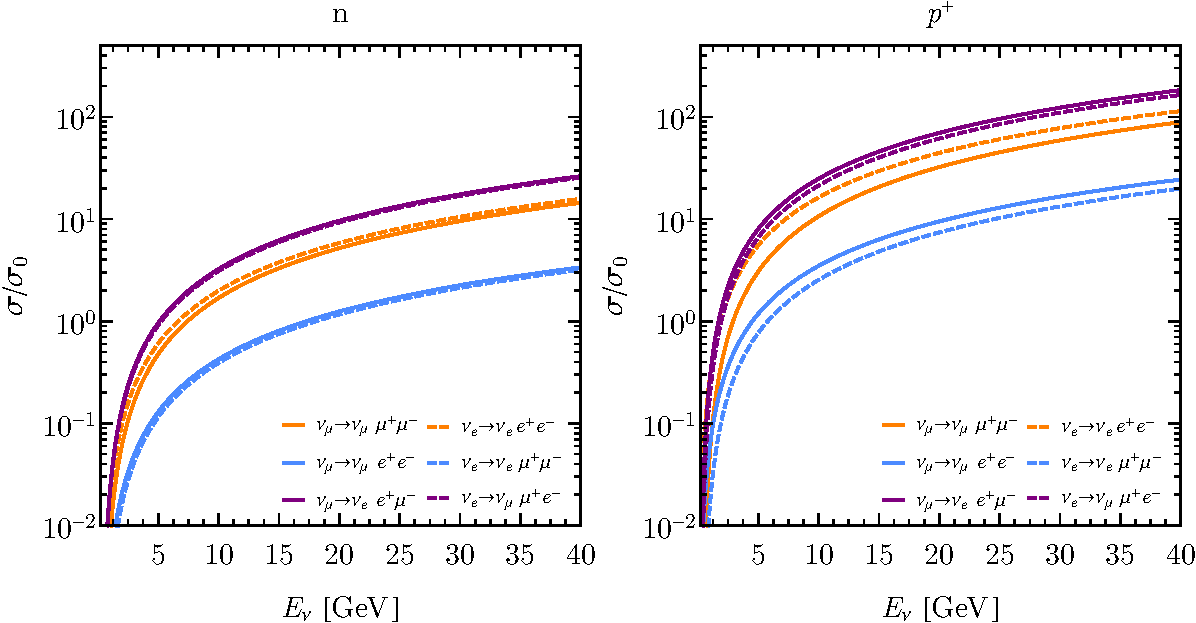
\includegraphics[width=\textwidth]{figs/Xsec_4PS_diff.pdf}
\caption[Incoherent neutrino trident production total cross sections.]{Cross sections for incoherent neutrino trident production on neutrons (left) and protons (right), including Pauli blocking effects as described in the text, normalized to $\sigma_0 =  10^{-44}$ cm$^2$. The full (dashed) lines correspond to the scattering of an incoming $\nu_\mu$ ($\nu_e$) produced by the NC (light-blue), CC (purple), and CC+NC (orange) SM interactions. \label{fig:dif_xsec}}
\end{figure}


%%%%%%%%%%%%%%%%%%%%%%%%%%%%%%%%%%%%%%%%%%%%%%%%%%%%
\subsection{Breakdown of the EPA \label{sec:EPAbreakdown}}

In order to understand the breakdown of the EPA in the neutrino trident case, let us first remind briefly the reader about the Weizs\"acker--Williams method of equivalent photons in Quantum Electrodynamics (QED)~\cite{vonWeizsacker:1934nji,Williams:1934ad}, and the main reason for its validity in that theory. The EPA, first introduced by E.\ Fermi~\cite{Fermi:1924tc}, is based on a simple principle: when an ultra-relativistic particle $P_i$ approaches a charged system $C_s$, like a nucleus, it will perceive the electromagnetic fields as nearly transverse, similar to the fields of a pulse of radiation, {\it i.e.},  as an on-shell photon. Therefore, it is possible to obtain an approximate total cross section for the inelastic scattering process producing a set of final particles $P_f$, $\sigma_{\rm t}(P_i + C_s \to P_f + C_s)$, by computing the scattering of the incoming particle with a real photon integrated over the energy spectrum of the off-shell photons,
%
\begin{align}
	\sigma_{\rm t}(P_i + C_s \to P_f + C_s)\approx\int\, dP(Q^2,\hat{s})\,\sigma_\gamma(P_i + \gamma \to P_f; \hat{s}, Q^2 = 0),
\end{align}
where the photo-production cross section for the process $P_i + \gamma \to P_f$, 
$\sigma_\gamma(P_i + \gamma \to P_f; \hat{s}, Q^2 = 0)$, 
depends on the center-of-mass energy of the $P_i$--photon system, $\sqrt{\hat{s}}$. Here $dP(Q^2,\hat{s})$ corresponds to the energy spectrum of the virtual photons, that is, the probability of emission of a virtual photon with transferred four-momentum $Q^2$ resulting in an center-of-mass energy $\sqrt{\hat{s}}$.
For trident scattering off a nuclear target, this probability can be approximated by~\cite{Belusevic:1987cw,Altmannshofer:2014pba}
\begin{align}\label{eq:GenEPA}
	dP(Q^2,\hat{s})=\frac{Z^2e^2}{4\pi^2}|F (Q^2)|^2\,\frac{d\hat{s}}{\hat{s}}\,\frac{dQ^2}{Q^2}\, .
\end{align}
A crucial fact in QED is that the cross section $\sigma_\gamma^{\rm QED}(P_i + \gamma \to P_f; \hat{s},0)$ is inversely proportional to $\hat{s}$,
\begin{align*}
	\sigma_\gamma^{\rm QED}(P_i + \gamma \to P_f; \hat{s},0) \propto \frac{1}{\hat{s}}\,.
\end{align*}
We see clearly that small values of $\hat{s}$ and consequently of the transferred four-momentum $Q^2$ dominate the cross section. Hence, the on-shell contribution is much more significant 
than the off-shell one, so the EPA will be valid and give the correct cross  section 
estimate for any QED process. 

Now, let us consider the case of neutrino trident production. In this case, the equivalent-photon cross section in the four-point interaction limit has a completely opposite dependence on the center-of-mass energy; it is \emph{proportional} to $\hat{s}$,
\begin{align*}
	\sigma_\gamma^{\rm FL}(P_i + \gamma \to P_f; \hat{s}, 0)\propto G_{\rm F}^2\, \hat{s}\, .
\end{align*}
This dependence is a manifestation of the unitarity violation in the Fermi theory. Therefore, we can see that for weak processes larger values of $\hat{s}$, and, consequently, larger values of $Q^2$ are more significant \cite{Kozhushner:1962aa, Shabalin:1963aa}.  The EPA is then generally not valid for the neutrino trident production, as the virtual photon contribution dominates over the real one. Nevertheless, one may wonder if there is a situation  in which the EPA can give a reasonable estimate for a neutrino trident process. 
As noticed in the early literature \cite{Kozhushner:1962aa, Shabalin:1963aa}, the presence of the nuclear form factor introduces a cut in the transferred momentum which, in turn, makes the EPA applicable for the specific case of the dimuon channel in the coherent regime. Let us discuss this in more detail. 

Recalling our exact decomposition, \refeq{eq:full_diff_xsec}, it is necessary to consider two assumptions for implementing the EPA \cite{Kozhushner:1962aa}:
%
\begin{enumerate} 
%
\item The longitudinal polarization contribution to the cross section can be neglected, i.e., $\sigma_{\nu\gamma}^\mathrm{L}(Q^2,\hat{s})\approx 0$;
%
\item The transverse polarization contribution to the cross section can be taken to be on-shell, i.e., $\sigma^\text{T}_{\nu\gamma}(Q^2,\hat{s}) \approx \sigma^\text{T}_{\nu\gamma}(0,\hat{s})$. 
%
\end{enumerate}
%
Assuming for now that these approximations hold, we can find a simplified expression for the coherent neutrino-target process, described by Eqs.~(\ref{eq:full_diff_xsec}) and (\ref{eq:hcoh}), in terms of the photon-neutrino cross section\footnote{An analogous expression can be obtained for the incoherent regime from Eq.~(\ref{eq:dcoh}).}:
%
\begin{align}     
\sigma_\text{EPA} = \frac{Z^2e^2}{4\pi^2}\int_{m_L^2}^{\hat{s}_{\rm max}} \frac{d\hat{s}}{\hat{s}}\,
\sigma^\mathrm{T}_{\nu\gamma}(0,\hat{s})
\int_{(\hat{s}/2E_\nu)^2}^{Q^2_{\rm max}}\frac{|F (Q^2)|^2}{Q^4} \left[ Q^2(1-y) - M_{\cal H}^2y^2\right]dQ^2\, , 
\end{align}
%
where we introduced the fractional change of the nucleus energy $y$, defined as $\hat{s} = (s-M_{\cal H}^2)y$, and the integration limits can be obtained from \eqref{eq:qslimts} after considering that $m_L^2\ll E_\nu M_{\cal H}$. Keeping only the leading terms in the small parameter $y$ \cite{Belusevic:1987cw}, we recover the EPA applied to the neutrino trident case
%
\begin{align} \label{eq:EPA_bad}
\sigma_\text{EPA} = \int \sigma^\mathrm{T}_{\nu\gamma}(0,\hat{s}) \, dP(Q^2,\hat{s})\, ,
\end{align}
%
where $dP(Q^2,\hat{s})$ is given in Eq.~(\ref{eq:GenEPA}). The EPA in the form of \refeq{eq:EPA_bad} has been used in trident calculations for the coherent dimuon channel \cite{Altmannshofer:2014pba} as well as for coherent mixed- and electron-flavour trident modes and incoherent trident modes \cite{Magill:2016hgc}.  Using our decomposition, we can explicitly compute both $\sigma^\mathrm{L}_{\nu \gamma}$ and $\sigma^\mathrm{T}_{\nu \gamma}$ and verify if the EPA conditions are satisfied for any channel and, if they are not, quantify the error introduced by making this approximation. For that purpose, we will compare the results of the full calculation, \refeq{eq:full_diff_xsec}, with the EPA results, \refeq{eq:EPA_bad}, by computing the following ratios in the physical region of the $(Q,\hat{s})$ plane,
\begin{align}\label{eq:ratios}
		\frac{\sigma^{\rm L}(Q^2,\hat{s})\,h_{\rm c}^{\rm L}(Q^2,\hat{s})}{\sigma^{\rm T}(Q^2,\hat{s})\,h_{\rm c}^{\rm T}(Q^2,\hat{s})}\, , \quad \frac{\sigma^\mathrm{T}_{\nu\gamma}(Q^2,\hat{s})}{\sigma^\mathrm{T}_{\nu\gamma}(0,\hat{s})}\, .
\end{align} 
The first ratio in Eq.\ \eqref{eq:ratios} will indicate where the longitudinal contribution can be neglected compared to the transverse one; while, the second ratio will show where the transverse contribution behaves as an on-shell photon. 

As an illustration of the general behaviour, we show in Fig.\ \ref{fig:4PSvsEPA} those ratios 
of cross sections for an incoming $\nu_\mu$ of fixed energy $E_\nu=3$ GeV colliding coherently with an $^{40}$Ar target, for the dielectron (left panels), mixed  (middle panels) and dimuon  (right panels)
channels. On the top panels of Fig.\ \ref{fig:4PSvsEPA} we see that the longitudinal component can be neglected for $Q\lesssim m_\alpha$, for the dielectron and dimuon channels, $\alpha=e,\mu$, while in the mixed case there is a much less pronounced hierarchy between the transverse and longitudinal components. On the bottom panels we have the comparison between on-shell and off-shell transverse photo-production cross sections. Again, we find that the EPA is only valid for $Q \lesssim m_\alpha$ for the dielectron and dimuon channels. For the mixed case, there is only a very small region in $Q < 10^{-2}$\,GeV for which the off-shell transverse cross section is comparable to the on-shell one. This relative suppression of the off-shell cross section can be understood by noticing that $Q$ enters the lepton propagators, suppressing the process for $Q \gtrsim m_\alpha$. For mixed channels it is then the smallest mass scale ($m_e$) that dictates the fall-off of the matrix element in $Q$, whilst the heaviest mass ($m_\mu$) defines the phase space boundaries, rendering most of this phase space incompatible with the EPA assumptions.   
%
\begin{figure}[t]
\centering
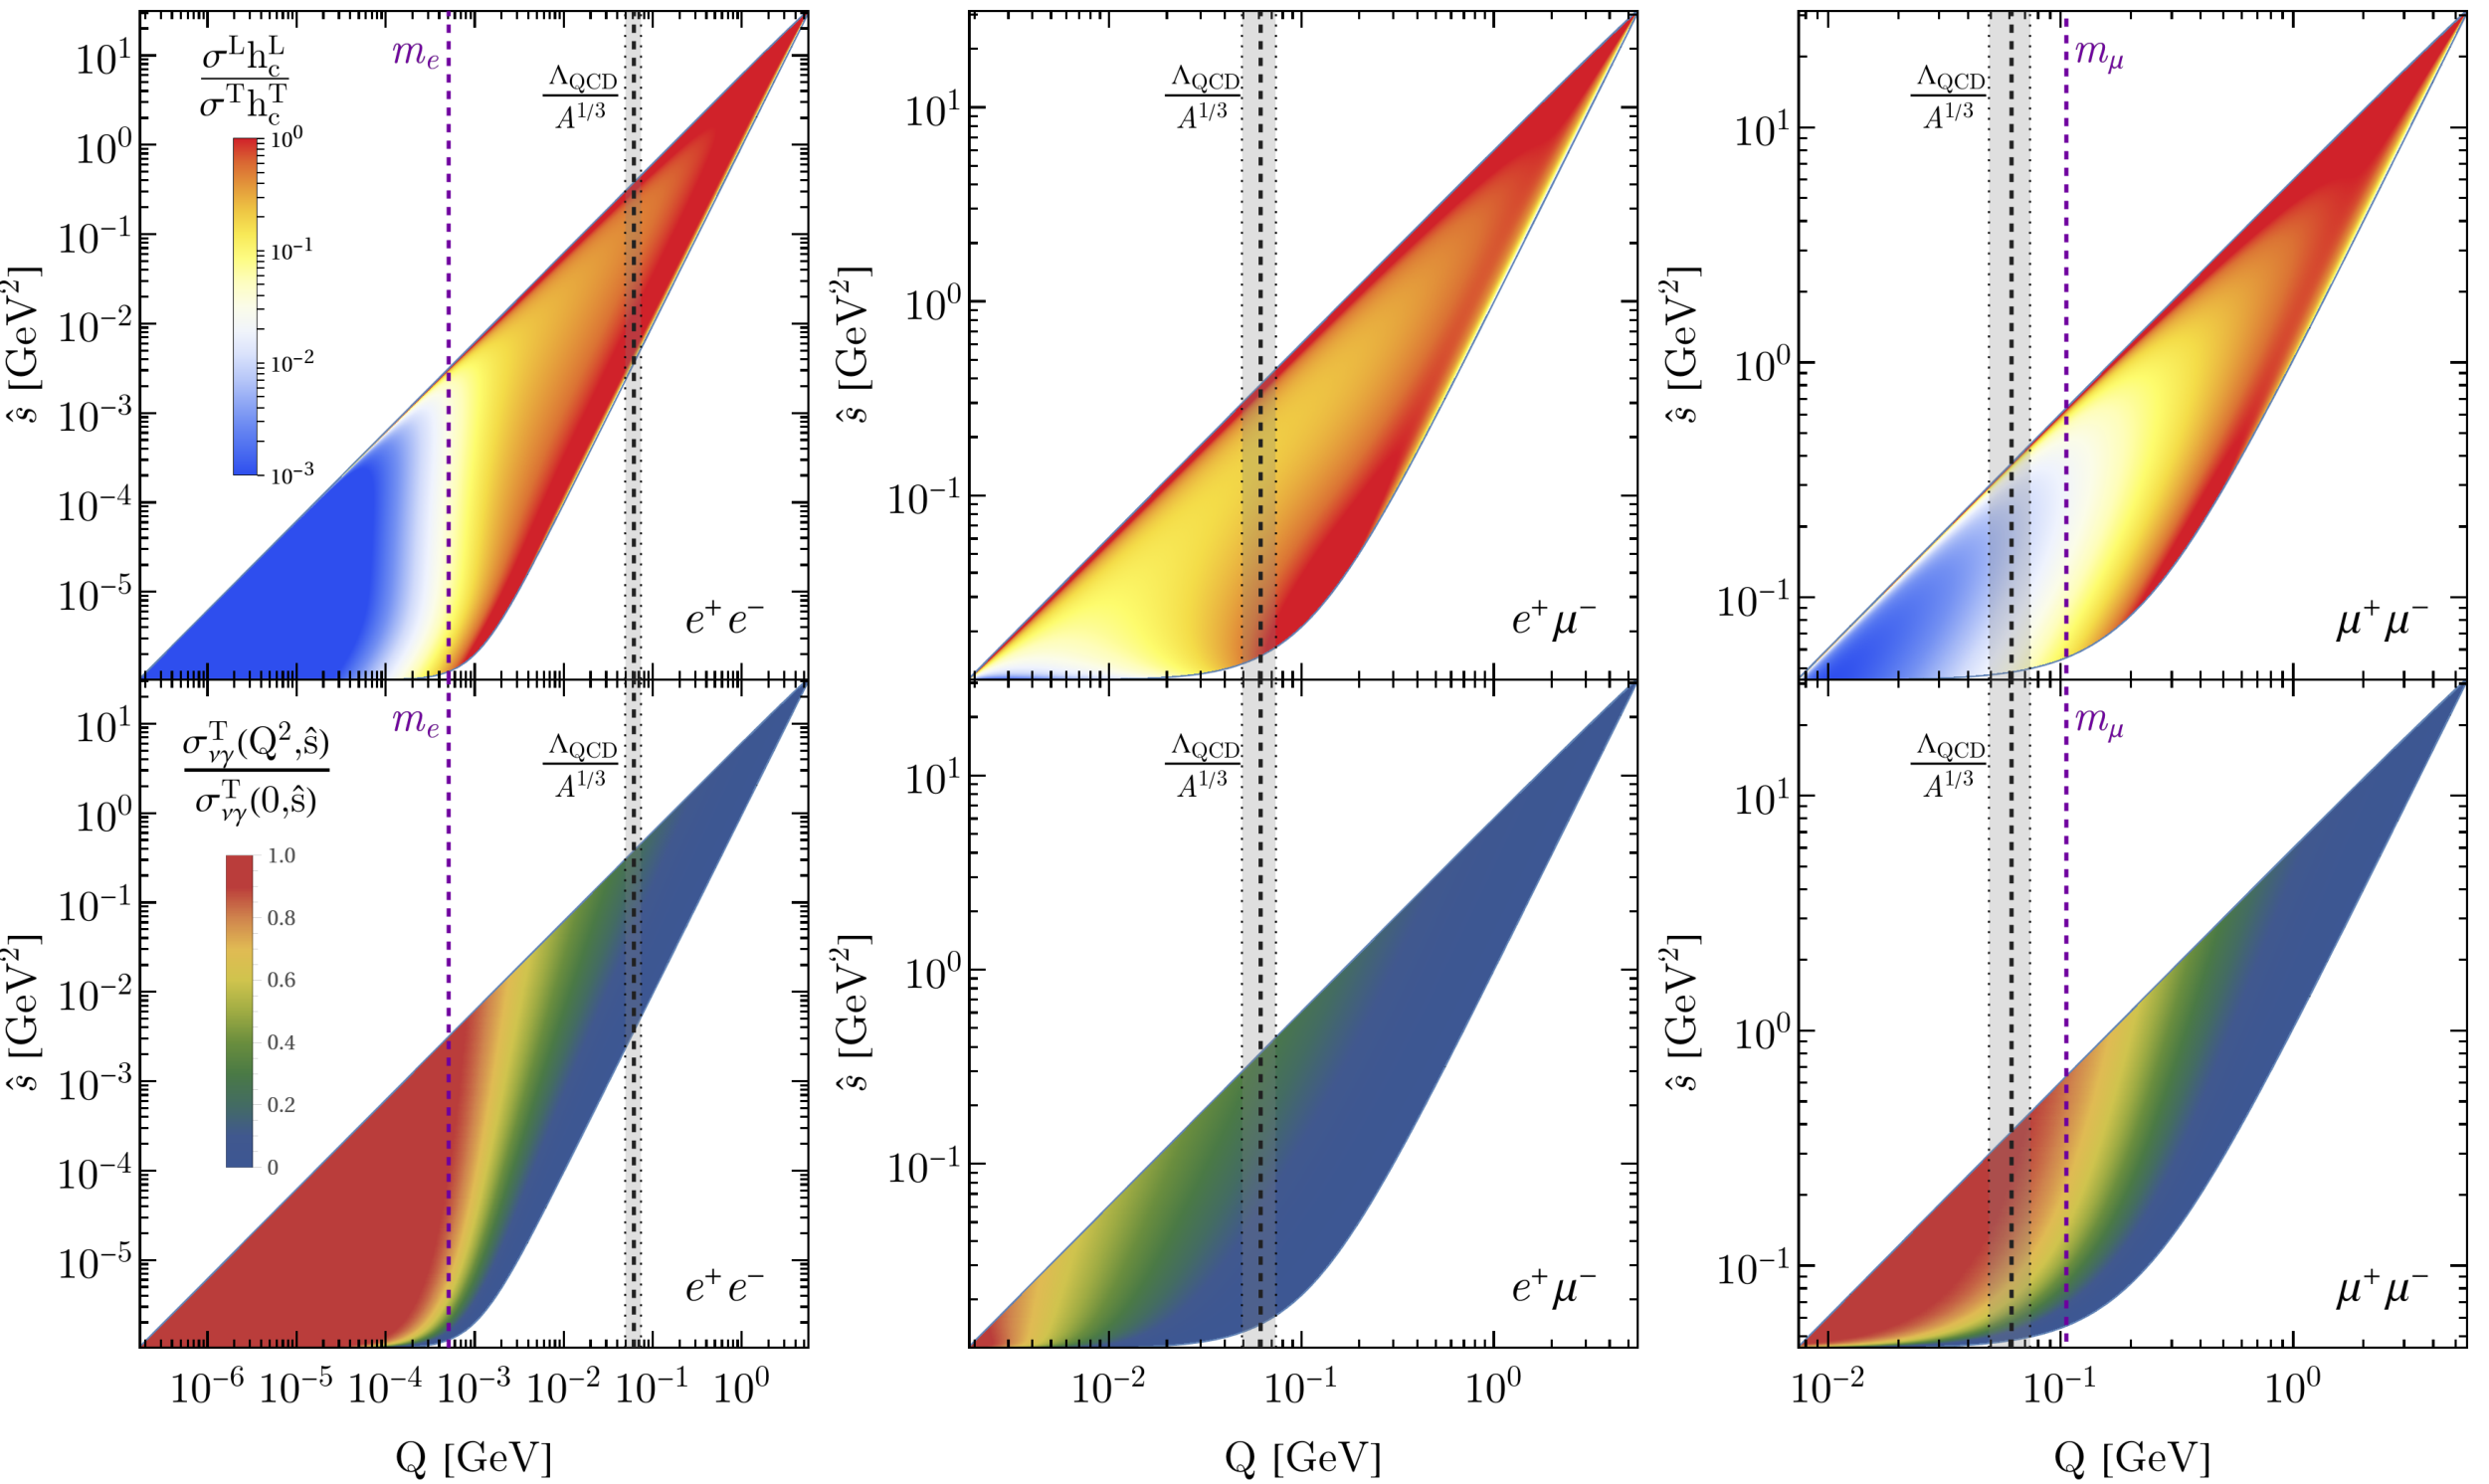
\includegraphics[width=\textwidth]{figs/4PS_vs_EPA.pdf}%
\caption[Comparison of the differential cross section using the EPA and using the full calculation for neutrino trident scattering.]{\label{fig:4PSvsEPA} Comparison between the full calculation of the trident production 
coherent cross section and the EPA in the kinematically allowed region of the $(Q,\hat{s})$ plane for an incoming $\nu_\mu$ with fixed energy $E_\nu=3$ GeV colliding with an $^{40}$Ar target. 
The left, middle and right panels correspond to the dielectron, mixed and dimuon final-states, respectively. The top panels correspond to the comparison between the longitudinal and transverse contributions while the bottom ones show the ratio between the transverse cross sections computed for an specific value of $Q$ with the cross section for an on-shell photon. The thick black dashed lines correspond to the cut in the $Q^2$ integration at $\Lambda_{\rm QCD}^2/ A^{2/3}$, and the shadowed region around these lines account for a variation of $20\%$ in the value of this cut. The purple dashed lines are for $Q=m_\alpha$, $\alpha=e,\mu$ for the unmixed cases.}
\end{figure}

These results explicitly show that the EPA is, in principle, not suitable for any neutrino trident process as it can overestimate the cross section quite substantially by treating the photo-production cross section at large $Q^2$ as on-shell. However, as previously mentioned, in the coherent regime the nuclear form factor introduces a strong suppression for large values of $Q^2$. In general, this dominates the behaviour of the cross sections for values of $Q^2$ smaller than the purely kinematic limit, $Q^2_{\rm max}$, and of the order of $\Lambda_{\rm QCD}/ A^{1/3}\approx 0.06$ GeV for coherent scattering on $^{40}$Ar. In the dimuon case, the latter scale happens to be smaller than the charged lepton masses, implying that the region where the EPA breaks down is heavily suppressed due to the nuclear form factor. The same cannot be said about coherent trident channels involving electrons, as the nuclear form factor suppression happens for much larger values of $Q$ than the EPA breakdown. Furthermore, for incoherent scattering the nucleon form factors suppress the cross sections only for much larger $Q$ values, $Q\approx 0.8$ GeV. The effective range of integration then includes a significant region where the EPA assumptions are invalid, leading to an overestimation of the incoherent cross section for every process regardless of the flavours of their final-state charged leptons. 

%
\begin{figure}[t]
	\centering
	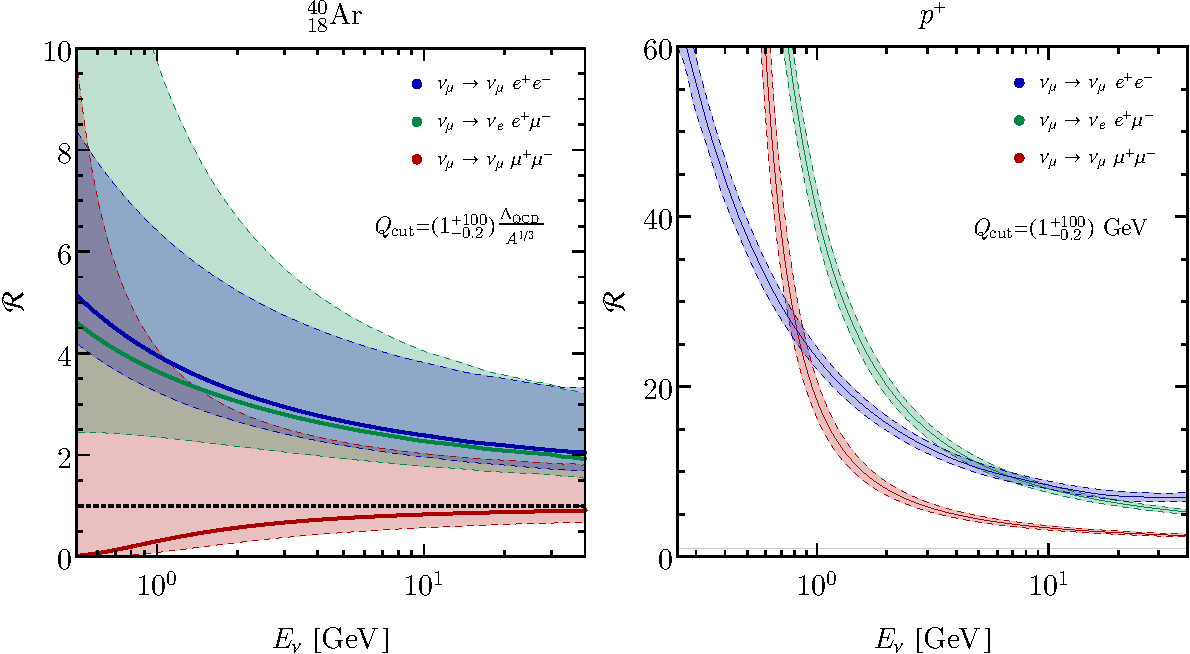
\includegraphics[width=\textwidth]{figs/XSec_ratio.pdf}%
	\caption[Comparison of the total cross section in the EPA and in the full calculation for neutrino trident scattering.]{\label{fig:comparison4PS_EPA} 
    Ratio $\mathcal{R}$ of the trident cross section calculated using 
    the EPA to the full four-body calculation. 
    Left panel: Ratio in the coherent regime on $^{40}$Ar. The full curves correspond to the central value of $Q_{\rm cut}$, and the upper (lower) boundary corresponds to a choice 100 times larger ($20\%$ smaller). 
Right  panel: Ratio in the incoherent regime for scattering on protons, where the full curves corresponds to the central value of $1.0$ GeV, and the upper (lower) boundary corresponds to a choice 100 times larger ($20\%$ smaller); we have taken the lower limit in the integration on $Q$ to match the choice of the coherent regime and we do not include Pauli blocking in these curves. A guide to the eye at $\mathcal{R} = 1$ is also shown.}
\end{figure}

In some calculations, artificial cuts have been imposed on the range of $Q^2$, affecting the validity of the EPA. In Ref. \cite{Magill:2016hgc}, it is claimed that to avoid double counting between different regimes, an artificial cut must be imposed, lowering the upper limit of integration in $Q^2$. Ref.~\cite{Magill:2016hgc} chooses a value of $Q^{\rm cut}_{\rm max} = \Lambda_{\rm QCD}/ A^{1/3}$ in the coherent regime (black thick dashed lines in Fig.\ \ref{fig:4PSvsEPA}), and $Q^{\rm cut}_{\rm min}= {\rm max}\left( \Lambda_{\rm QCD}/ A^{1/3}, \hat{s}/2E_\nu\right)$ and $Q^{\rm cut}_{\rm max} = 1.0$ GeV in the incoherent regime. We believe that no such cut is required on physical grounds\footnote{It should be noted that the coherent and incoherent regimes have different phase space boundaries and that the form factors should guarantee their independence.}, and their presence will impact the EPA cross section quite dramatically. Let us first consider the dimuon case in the coherent regime, where the EPA assumptions hold reasonably well in the relevant parts of phase space. By introducing a value for $Q^{\rm cut}_{\rm max}$ we would be decreasing the total relevant phase space for the process, reducing the total cross section. Therefore, despite the EPA tendency to overestimate the cross section in this channel, an artificial cut in $Q^2$ can actually lead to an underestimation of the cross section. In the electron channels, where the EPA breakdown is much more dramatic, we can expect that the overestimation of the cross section by the EPA is reduced by the cut $Q^{\rm cut}_{\rm max}$. In fact, one way to improve the EPA for the dielectron channel is to artificially cut on the $Q^2$ integral around the region where the ap\-pro\-xi\-ma\-tion breaks down \cite{Frixione:1993yw}. This cut does then improve the coherent EPA calculation by decreasing the overestimation of the cross section. However, an energy independent cut cannot provide a good estimate of the cross section over all values of $E_\nu$. To illustrate our point and to quantify the errors induced by the EPA, we show on the left panel of \reffig{fig:comparison4PS_EPA} the ratio $\mathcal{R}$ of the trident cross section calculated using the EPA with an artificial cut at $Q^2_\text{cut}$, as performed in \cite{Magill:2016hgc}, to the full calculation used in this work as a function of the incoming neutrino energy:
%
 \begin{equation}
 \mathcal{R} = \frac{\sigma_{\rm EPA} (E_\nu) \vert_{Q_{\rm cut}}}{\sigma_{\rm 4PS} (E_\nu)}\,.
 \end{equation}
%
 In this plot we vary the artificial cut on $Q^2$ around the choice of \cite{Magill:2016hgc} (shown as the central dashed line) in two ways. First we reduce it by $20 \%$, and then increase it by a large factor, recovering the case with no $Q^2$ cut. From this, our conclusions about the validity of the approximation are confirmed, and it becomes evident that the trident coherent cross section is very sensitive to the choice of $Q^2_{\mathrm{cut}}$. In particular, the EPA with all the assumptions that lead to \refeq{eq:EPA_bad} and the absence of a $Q^2$ cut can lead to an overestimation of all trident channels, including the dimuon one. Once the cut is implemented, however, the approximation becomes better for the dimuon channel, but still unacceptable for the electron ones. It is also clear that an energy independent cut cannot give the correct cross section at all energies. This is particularly troublesome for detectors subjected to a neutrino flux covering a wide energy range such as the near detectors for DUNE and  MINOS or MINER$\nu$A. Moreover, \refeq{eq:EPA_bad} fails at low energies, and generally, overestimates the coherent cross sections by at least  200\%. At these energies, one must be wary of the additional approximations in \refeq{eq:EPA_bad} regarding the integration limits and the small $y$ limit.     

On the right panel of \reffig{fig:comparison4PS_EPA} we illustrate what happens in the incoherent regime, where the nucleon form factors impact the cross section at much larger values of $Q^2$ and have a slower fall-off. We see that the incoherent cross section is dramatically overestimated over the full range of $E_\nu$ considered and for any trident mode. The discrepancy is particularly important for $E_\nu \lesssim$ 5 GeV and larger than in the coherent regime by at least an order of magnitude\footnote{There are some differences in the treatment of the hadronic system between the EPA calculation in \cite{Magill:2016hgc} and the one presented here. However, these differences are of the order 10\% to 20\%. Note also that we do not implement any Pauli blocking when calculating $\mathcal{R}$ to avoid ambiguities over the choice of the range of $Q^2$.}. We also see that the cuts on $Q^2$ impact the EPA calculation much less dramatically, and that its use is unlikely to yield the correct result.

Given these problems with both coherent and incoherent cross section calculations due to the breakdown of the EPA for trident production, in what follows we will use the complete four-body calculation.

%%%%%%%%%%%%%%%%%%%%%%%%%%%%%%%%%%%%%%%%%%%%%%%%%%%%
\subsection{Coherent versus incoherent Scattering in Trident Production}
\label{subsec:cohdiff}

%
\begin{figure}[t]
	\centering
	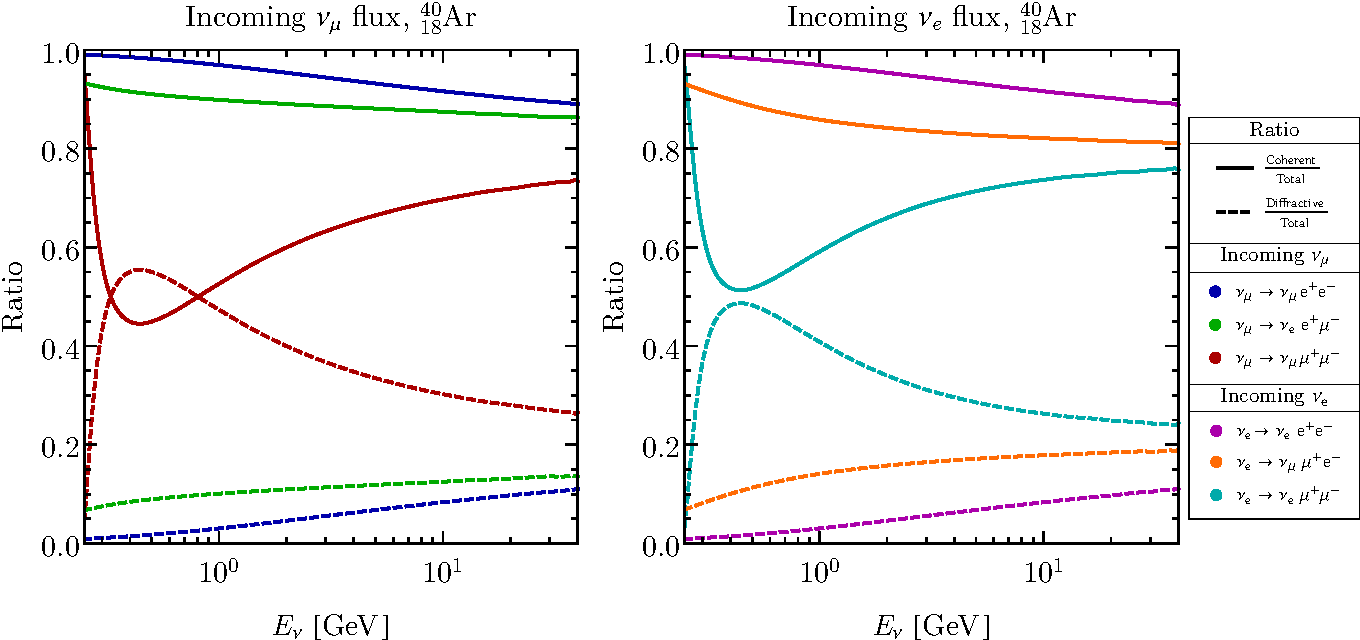
\includegraphics[width=\textwidth]{figs/Ratio_CDvsT.pdf}%
	\caption[Ration between coherent and incoherent trident total cross sections.]{\label{fig:RatioCDvsT} On the left (right) panel we show the
    ratio of the coherent (full lines) and the incoherent (dashed lines) contributions to the total trident cross section for an incoming flux of $\nu_\mu$($\nu_e$) as a function of $E_\nu$ for an 
    $^{40}$Ar target.}
\end{figure}
%

Let us  now comment on the significance of  the coherent and incoherent contributions to the total cross for the different trident channels. 
In Fig.\ \ref{fig:RatioCDvsT} we present the ratio of the coherent and the incoherent scattering cross sections to the total cross section for an $^{40}$Ar target for an incoming $\nu_\mu$ (left) and $\nu_e$ (right)  neutrino. We can see that the coherent regime dominates at all neutrino energies when there is an electron in the final-state, especially in the dielectron case. 
This can be explained by noting that the $Q^2$ necessary to create an electron pair is smaller than the one needed to create a muon; thus, coherent scattering is more likely to occur for this mode. Conversely, 
as one needs larger momentum transferred to produce a muon (either accompanied by an electron 
or another muon) the  incoherent regime becomes more likely in these modes, as we can explicitly 
see in Fig.\ \ref{fig:RatioCDvsT}. 
Because of this effect the incoherent contribution is $\lesssim$ 10\%, except for the 
dimuon channel where it can be between $30$ and $40$\% in most of the energy region.
Furthermore, when we compare the two incoming types of neutrinos, we see that for an incoming $\nu_\mu$ the incoherent contribution is larger than the coherent one in the range $0.3\ {\rm GeV}\lesssim E_\nu \lesssim 0.8$ GeV, while for an incoming $\nu_e$ this never happens. 
This difference can be explained by the fact that CC and NC contributions  are simultaneously present for the scattering of an initial $\nu_\mu$ creating a muon pair, whereas
for an initial $\nu_e$ creating a muon pair, we will only have the NC contribution, see Table \ref{tab:tridentmodes}.

An important difference between the coherent and incoherent regimes will be in their hadronic signatures in the detector. Neutrino trident production is usually associated with zero hadronic energy at the vertex, a feature that proved very useful in reducing backgrounds in previous measurements. Whilst this is a natural assumption for the coherent regime, it need not be the case in the incoherent one. In fact, in the latter it is likely that the struck nucleon is ejected from the nucleus in a significant fraction of events with $Q$ exceeding the nuclear binding energy
%
\footnote{The peak of our incoherent $Q^2$ distributions happens at around $Q \approx 300$ MeV, much beyond the typical binding energy for Ar (see \refapp{app:distributions}). Without Pauli suppression, however, we expect this value to drop.}. Since the dominant incoherent contribution comes from scattering on protons, these could then be visible in the detector if their energies are above threshold. On the other hand, the struck nucleon is subject to many nuclear effects which may significantly affect the hadronic signature, such as interactions of the struck nucleon in the nuclear medium as well as reabsorption. Our calculation of Pauli blocking, for example, shows large suppressions ($\sim 50\%$) precisely in the low $Q^2$ region, usually associated with no hadronic activity. This then raises the question of how well one can predict the hadronic signatures of incoherent events given the difficulty in modelling the nuclear environment. We therefore do not commit to an estimate of the number of incoherent events that would have a coherent-like hadronic signature, but merely point out that this might introduce additional uncertainties in the calculation, especially in the $\mu^+ \mu^-$ channel where the incoherent contribution is comparable to the coherent one. Finally, from now on we will refer to the number of trident events with no hadronic activity as coherent-like, where this number can range from coherent only to coherent plus all incoherent events. 


%%%%%%%%%%%%%%%%%%%%%%%%%%%%%%%%%%%%%%%%%%%%%%%%%%%%
\section{Trident Events in LAr Detectors}
\label{sec:LAr}

In this section we calculate the total number of expected  trident events for some present and future LAr detectors with different fiducial masses, total exposures and beamlines. In Table~\ref{tab:LAr} we specify the values used for each set-up and in Fig.~\ref{fig:LAr} we show the total production cross section for each neutrino trident mode of Table~\ref{tab:tridentmodes}
as well as the neutrino fluxes as a function of $E_\nu$ at the position of each experiment.  

%%%%%%%%%%%%%%%%%%%%%%%%%%%%%%%%%%%%%%%%%%%%%%%%%%%%
\subsection{Event Rates}
\label{subsec:rates}

The total number of trident events, $N^{\text{\Neptune}}_{\rm X}$, expected for a given trident mode at any detector is written as  
\begin{eqnarray}
\label{eq:nevents}
N^{\text{\Neptune}}_{\rm X}={\rm Norm}\times\int dE_\nu \, \sigma_{\nu {\rm X}}(E_\nu) \frac{d\phi_{\nu}(E_\nu)}{dE_\nu}\epsilon(E_\nu)\,,
\end{eqnarray}
where $\sigma_{\nu {\rm X}}$ can be the trident total (${\rm X}={\cal N}$), coherent ($\mathrm{X=c}$) or incoherent ($\mathrm{X=d}$) cross sections 
for a given mode, $\phi_{\nu}$ is the flux of the incoming neutrino and $\epsilon(E_\nu)$ is the efficiency of detection of the charged leptons. In the calculations of this section, we assume an efficiency of $100\%$\footnote{See \refsec{subsec:kine} for a discussion on the detection efficiencies for trident events and backgrounds.}.
%
The normalization is calculated as 
 %
$${\rm Norm}= {\rm{Exposure}}~[{\rm{POT}}] \times \frac{{\rm{Fiducial~Detector~Mass}\times N_A}}{m_{\rm T}} \left[{\rm{target~particles}}\right],$$
%%
where $m_{\rm T}$ is the molar mass of the target particle and $N_A$ is Avogadro's number.
%
Two features of the cross sections are important for the event rate calculation: 
threshold effects, especially for channels involving muons in the final-state,
and cross section's growth with energy. In particular, we expect higher trident event rates for experiments with higher energy neutrino beams. 

We start our study with the three detectors of the SBN program, one of which, $\mu$BooNE, is already installed and taking data at Fermilab. These three LAr time projection chamber detectors are located along the Booster Neutrino Beam line which is by now a well-understood source, having the focus of active research for over 15 years. 
%
Although the number of trident events expected in these detectors is rather low, they may offer one of the first opportunities to study trident events in LAr, as well as to better understand their backgrounds in this medium and to devise improved analysis techniques.
%
After that we study the proposed near detector for DUNE. This turns out to be the most important LAr detector for trident production since it will provide the highest number of events in both neutrino and antineutrino modes. 
%
Finally, having in mind the novel flavour composition of neutrino beams from muon facilities, we investigate trident rates at a 100~t LAr detector for the $\nu$STORM project. This last facility could offer a very well understood neutrino beam with as many electron neutrinos as muon antineutrinos from muon decays, creating new possibilities for trident scattering measurements.
%%
\begin{table}[t]
\begin{center}
\scalebox{0.9}{
\begin{tabular}{|cccccc|}
\hline\hline
		\bf Channel & \bf SBND& \bf $\mu$BooNE & \bf ICARUS & \bf DUNE ND &\bf  $\nu$STORM ND \\ \hline \hline
		$\nu_\mu\to\nu_e e^+ \mu^-$& $10$ &$0.7$ &$1$ &$2844 ~ (235)$ & $159$ \\
        &$1$ &$0.08$ &$0.1$ &$369 ~ (33)$& $18$\\\hline
        $\overline\nu_\mu\to\overline\nu_e e^- \mu^+$&$0.4$ &$0.02$ &$0.04$ &$122~(2051)$ & $23$\\
        &$0.04$ &$0.003$ &$0.004$ &$16~(262)$ & $3$\\\hline
	$\nu_e\to\nu_\mu e^- \mu^+$& $0.05$ &$0.003$ &$0.004$ &$22~(7)$ & $9$\\
        &$0.008$ &$0.0005$ &$0.0008$ &$5~(1)$ & $2$\\\hline
	$\overline\nu_e\to\overline\nu_\mu e^+ \mu^-$& $0.005$ &$0.0003$ &$0.0005$ &$5~(14)$ & $-$\\
    &$0.001$ &$0.0001$ &$0.0001$ &$1~(3)$ & $-$\\\hline
    \hline\hline
    {$\rm{Total} \ e^\pm \mu^\mp$}& $10$ &$0.7$ &$1$ &$2993~(2307)$ & $191$ \\
    &$1$ &$0.1$ &$0.1$ &$391~(299)$ & $23$\\\hline
    \hline
		$\nu_\mu\to\nu_\mu e^+ e^-$& $6$ &$0.4$ &$0.7$ &$913~(58)$ & $73$ \\
        &$0.2$ &$0.04$ &$0.02$ &$57~(5)$ & $3$\\\hline
        $\overline\nu_\mu\to\overline\nu_\mu e^- e^+$& $0.2$ &$0.01$ &$0.02$ &$34~(695)$ & $9$\\
        &$0.01$ &$0.001$ &$0.002$ &$2~(41)$ & $0.5$\\\hline
	$\nu_e\to\nu_e e^- e^+$&$0.2$ &$0.01$ &$0.02$ &$50~(13)$ & $32$ \\
    &$0.01$ &$0.001$ &$0.002$ &$4~(1)$ & $2$\\\hline
	$\overline\nu_e\to\overline\nu_e e^+ e^-$&$0.02$ &$0.001$ &$0.002$ &$10~(34)$ & $-$ \\
    &$0.0009$ &$0.0001$ &$0.0002$ &$1~(2)$ & $-$\\\hline
    \hline\hline
    ${\rm{Total}}\  e^+ e^-$& $6$ &$0.4$ &$0.7$ &$1007~(800)$ & $114$\\
    &$0.2$ &$0.0$ &$0.02$ &$64~(49)$ & $6$\\\hline
    \hline    
		$\nu_\mu\to\nu_\mu \mu^+ \mu^-$& $0.4$ &$0.03$ &$0.04$ &$271~(32)$ & $9$ \\
        &$0.3$ &$0.03$ &$0.04$ &$135~(14)$ & $5$\\\hline
        $\overline\nu_\mu\to\overline\nu_\mu \mu^- \mu^+$& $0.01$ &$0.001$ &$0.001$ &$14~(177)$ & $2$\\
        &$0.01$ &$0.0009$ &$0.001$ &$7~(93)$ & $1$\\\hline
 $\nu_e\to\nu_e \mu^+ \mu^-$    &$0.002$ &$0.0001$ &$0.0001$ &$1~(0.5)$ & $0.4$\\  
 &$0.001$ &$0.0001$ &$0.0001$ &$0.5~(0.2)$ & $0.2$\\\hline
        $\overline\nu_e\to\overline\nu_e \mu^+ \mu^-$&$0.0002$ &$0.0000$ &$0.0000$ &$0.3~(0.9)$ & $-$\\
        &$0.0001$ &$0.0000$ &$0.0000$ &$0.1~(0.3)$ & $-$\\\hline
        \hline\hline
    ${\rm{Total}} \ \mu^+ \mu^-$ &$0.4$ &$0.0$ &$0.0$ &$286~(210)$ & $11$ \\
    &$0.3$ &$0.0$ &$0.0$ &$143~(108)$ & $6$\\
    \hline\hline
\end{tabular}}
\end{center}
\caption[Trident rates in LAr detectors.]{\label{tab:LArrates}Total number of \textbf{coherent} (top row) and \textbf{incoherent} (bottom row) trident events expected at different LAr experiments for a given channel.
The numbers in parentheses are for the antineutrino running mode, when present. These calculations  
considered a detector efficiency of 100\%. }
\end{table}
%%%%%%%%%%%%%%%%%%%%%%%%%%%%%%%%%%%%%%%%%%%%%%%%%%%%
\paragraph{The SBN Program}

The SBN Program at Fermilab is a joint endeavour by three collaborations ICARUS, $\mu$BooNE and 
SBND to perform searches for eV-sterile neutrinos and study neutrino-Ar cross sections \cite{SBNproposal}. As can be seen in Tab.~\ref{tab:LAr}, SBND has the shortest baseline (110 m) and therefore the largest neutrino fluxes (shown in Fig.~\ref{fig:LAr} and taken from Fig. 3 of \cite{SBNproposal}). The largest detector, ICARUS, is also the one with the longest baseline (600 m) and consequently subject to the lowest neutrino fluxes.
%
The ratio between the fluxes at the different detectors are  $\phi_{\mu\rm{BooNE}}/\phi_{\rm{SBND}}=5$\% and $\phi_{\rm{ICARUS}}/\phi_{\rm{SBND}}=3$\%.
%
The neutrino beam composition is about 93\% of $\nu_\mu$,  6\% of $\overline\nu_\mu$ and  
$1\%$ of $\nu_e+\overline{\nu}_e$. 

Considering the difference in fluxes and the total number of targets in each of these 
detectors, one can estimate the following ratios of trident events: 
${N^\text{\Neptune}_{\mu\rm{BooNE}}}/{N^\text{\Neptune}_{\rm{SBND}}}\sim 8$\% and ${N^\text{\Neptune}_{\rm{ICARUS}}}/{N^\text{\Neptune}_{\rm{SBND}}}\sim 10$\%. Unfortunately, 
since the fluxes are peaked at a rather low energy ($E_\nu \lesssim 1$ GeV), where the trident  
cross sections are still quite small ($\lesssim 10^{-42}$ cm$^2$) we expect very few 
trident events produced.
%
The exact number of trident events for those detectors according to our calculations is 
presented in Tab.~\ref{tab:LArrates}. For each trident channel the first (second) row
shows the number of coherent (incoherent) events. As expected, less than a total 
of 20 events across all channels can be detected by SBND, and a negligible rate of events is expected at $\mu$BooNE and ICARUS. 

%%%%%%%%%%%%%%%%%%%%%%%%%%%%%%%%%%%%%%%%%%%%%%%%%%%%
\paragraph{DUNE Near Detector} The DUNE experiment will operate with neutrino as well as antineutrino LBNF beams produced by 
directing a 1.2 MW beam of protons onto a fixed target \cite{Acciarri:2016ooe,DUNECDRvolII}. 
The design of the near detector is not finalised, but the current designs favour a mixed technology  detector combining a LAr TPC with a larger tracker module.  In this work, we will assume that DUNE ND is a LAr detector located at $574$ m from the target with a fiducial mass of 50~t \cite{WeberTalk}. As the trident event rate scales with the density of the target, any tracker module will not significantly influence the total event rate, and does not feature in our estimates; although, its presence is assumed to improve reconstruction of final-state muons. Our estimates can be easily scaled for the final design by using \refeq{eq:nevents}.

For the first 6 years of data taking (3 years in the neutrino plus 3 years in the antineutrino 
mode) the collaboration expects $1.83\times 10^{21}$~POT/year with  a plan to upgrade the beam after the 6th year for 2 extra years in each beam mode  with double exposure, making a total of $1.83 \times(3+2\times2)\times 10^{21}~{\rm{POT}}$ for each mode \cite{DUNE:exposure}. We will 
assume the total 10-year exposure in our calculations.
%
. as the relevant fluxes at the DUNE ND location (see Fig.~\ref{fig:LAr}). The beam composition of the neutrino (antineutrino) beam is about 96\% $\nu_\mu$ ($\overline\nu_\mu$), 4\%  $\overline\nu_\mu$ ($\nu_\mu$) and 1\% $\nu_e+\overline\nu_e$.
 
The number of trident events for DUNE ND can be found in Tab.~\ref{tab:LArrates}. 
The numbers in parentheses correspond to antineutrino beam mode.
Note that although the trident cross sections are the same 
for neutrinos and antineutrinos, the fluxes are a bit lower for the antineutrino beam, as a consequence we predict a lower event rate for this beam\footnote{A similar difference will apply to the processes constituting the background to the trident process, although there is an additional suppression in many channels due to the lower antineutrino cross sections.}.
%
Due to the much higher energy and wider energy range of the neutrino fluxes at DUNE ND, as compared to the SBN detectors, DUNE can observe a considerable number of trident events, about 300 times the number of trident events expected for SBND just in the neutrino mode. Moreover, the subdominant component of 
each beam mode will also contribute to the signal. For example, we expect to observe $2051$ trident events in the $\overline{\nu}_\mu\to\overline{\nu}_e e^- \mu^+$ channel in the antineutrino mode. However, we also expect 
$235$ events in the $\nu_\mu\to\nu_e e^+ \mu^-$ channel produced by 
the subdominant component of $\nu_\mu$ in the antineutrino beam.
%
We have considered 100\% detection efficiency here, however, we will see in Sec.~\ref{subsec:bck} that after implementing hadronic vetos, detector thresholds and kinematical cuts to substantially reduce the background we expect an efficiency of about 47\%-65\% on coherent tridents, depending on the channel (see Tab.~\ref{tab:DUNE_ND_NU_BG}).

The mixed flavour trident channel is the one with the highest statistics (more than 6000 events adding 
neutrino and antineutrino beam modes), 11\% of which are produced by incoherent scattering. The dielectron channel comes next with a total of a bit more than 1900 events, 5\%  of which are produced by incoherent scattering. Although the  dimuon channel is the less copious one, with only about 
750 events produced, almost 34\% of these events are produced by a incoherent process.
This can be understood by recalling our discussions in Sec.~\ref{subsec:cohdiff}.

Finally, we note that a dedicated high-energy run at DUNE has been mooted, to be undertaken after the full period of data collecting for the oscillation analysis. Thanks to the higher energies of the beam, this has the potential to see a significant number of neutrino tridents, provided it can collect enough POTs.  

%%%%%%%%%%%%%%%%%%%%%%%%%%%%%%%%%%%%%%%%%%%%%%%%%%%%
\paragraph{$\nu$STORM} In this section we study the trident rates for a possible LAr detector for the proposed 
$\nu$STORM experiment \cite{Soler:2015ada,nuSTORM2017}. The $\nu$STORM facility 
is based on a neutrino factory-like design and has the goal to search for sterile neutrinos and study neutrino nucleus cross sections \cite{Adey:2014rfv}. Although this proposal is in its early days, $\nu$STORM has the potential to make cross section measurements with unprecedented precision. In its current design, $120$-GeV protons are used to produce pions from a fixed target with the pions subsequently decaying into muons and neutrinos. The muons are captured in a storage ring and during repeated passes around the ring they decay to produce neutrinos.
%
Consequently, the storage ring is an intense source of three types of neutrino
flavours: $\nu_\mu$ from $\pi^+$ and $K^+$ decays, which will be more than $99\%$ of the total flux, $\nu_e$ and $\overline\nu_\mu$ from recirculated muon decays which will comprise less than $1\%$ of the total flux. An important point, however, is that the neutrinos coming from the pion and kaon decays can be separated by event timing from the ones produced by the stored muons. This distinction allows the $\nu_\mu$ flux to be studied almost independently from the $\overline{\nu}_\mu$ and $\nu_e$ flux. In addition, it implies after the initial flash of meson-derived events, that the flux consists of as many electron neutrinos as muon antineutrinos. We will assume a LAr detector for $\nu$STORM at a baseline of 50\,m with 100\,t of fiducial mass with an exposure of $10^{21}$ POT. The neutrino fluxes, assuming 
a central $\mu^+$ momentum of $3.8$~GeV/c in the storage ring, are taken from Ref.~\cite{nuSTORM2017} and are 
shown in Fig.~\ref{fig:LAr}.

In Tab.~\ref{tab:LArrates}, we show the results of our calculations for $\nu$STORM. 
More than $97\%$ of the events from the incoming $\nu_\mu$ are from pion decays and only less 
than $3\%$ from kaon decays. Since we only consider the decay of mesons with positive charges and we expect neutral and wrong charge contamination to be small, we do not have trident events from incoming $\overline\nu_e$.
%
The total number of mixed flavour, dielectron and dimuon channel events is, respectively,
214, 120 and 17, much less than what can be achieved at the larger neutrino energies available at the DUNE ND. The novel flavour structure of the beam does enhance the contribution of $\nu_e$ induced tridents with respect to the $\pbar{\nu}_\mu$ ones, but this contribution only becomes dominant for the $e^+e^-$ tridents in the muon decay events. Finally, we emphasize that the experimental design parameters for $\nu$STORM are far from definite. Increasing the energy of stored muons and the size of the detector are both viable options which could significantly enhance the rates we present.

%

%%%%%%%%%%%%%%%%%%%%%%%%%%%%%%%%%%%%%%%%%%%%%%%%%%%%
\subsection{Background Estimates for Neutrino Trident in LAr}
\label{subsec:bck}

The study of any rare process is a struggle against both systematic uncertainties in the event rates and unavoidable background processes. True dilepton signatures are naturally rare in neutrino scattering experiments, but with modest rates of particle misidentification a non-trivial background arises. In this section we estimate the background to trident processes in LAr and its impact on the trident measurement. We perform our analysis only for DUNE ND, in neutrino and antineutrino mode, but our results are expected to be broadly applicable to other LAr detectors. We have generated a sample of $1.1 \times 10^6$ background events using GENIE \cite{Andreopoulos2009} for incident electron and muon flavour neutrinos and antineutrinos. It is worth noting, however, that this event sample will in fact be smaller than the total number of neutrino interactions expected in the DUNE ND. 
%
Our goal, therefore, will be to demonstrate that with modest analysis cuts background levels can be suppressed significantly such that they become comparable to or smaller than the signals we are looking for. In the absence of events that satisfy our background definition, we argue that the frequency of that type of event is less than one in $1.1\times 10^6$ interactions of the corresponding initial neutrino.  

To account for misreconstruction in the detector, we implement resolutions as a gaussian smear around the true MC energies and angles. We assume relative energy resolutions as $\sigma/E = 15\%/\sqrt{E}$ for $e/\gamma$ showers and protons, and $6\%/\sqrt{E}$ for charged pions and muons. Angular resolutions are assumed to be $1^\circ$ for all particles (proton angles are never smeared in our analysis). The detection thresholds are a crucial part of the analysis, since for many channels one ends up with very soft electrons. We take thresholds to be $30$ MeV for muons and $e/\gamma$ showers kinetic energy, $21$ MeV for protons and $100$ MeV for $\pi^{\pm}$ \cite{DUNECDRvolII}.

%%%%%%%%%%%%%%%%%%%%%%%%%%%%%%%%%%%%%%%%%%%%%%%%%%%%
\subsubsection{Background Candidates}
\label{subsubsec:misID}
We focus on three final-state charged lepton combinations: $\mu^+\mu^-$, $\mu^\pm e^\mp$ and $e^+e^-$. Genuine production of these states is possible in background processes, but usually rare, deriving from meson resonances or other prompt decays. The majority of the background is expected to be from particle misidentification (misID). We assume that protons can always be identified above threshold and that neutrons leave no detectable signature in the detector. In addition, we require no charge ID capabilities from the detector and assume that the interaction vertex can always be reconstructed. Under these assumptions, we have incorporated three misidentifications which will affect our analysis, and give our naive estimates for their rates in Tab.~\ref{tab:misIDlist}. Any other particle pairs are assumed to be distinguishable from each other when needed.
%
\renewcommand{\arraystretch}{1.2}
\begin{table}[t]
\centering 
\begin{tabular}{|c c|}
\hline\hline
\bf misID & \bf Rate \\
\hline\hline
%
$\gamma$ as $e^\pm$ & 0.05 \\
\hline
\multirow{2}{*}{$\gamma$ as $e^+e^-$} & 0.1 (w/ vertex)  \\
%\cline{2-2}
 & 1 (no vertex + overlapping)  \\
\hline
$\pi^\pm$ as $\mu^\pm$ & 0.1 \\
\hline\hline
\end{tabular}
\caption[Rates for particle misID in LAr.]{\label{tab:misIDlist} Assumed misID rates for various particles in a LAr detector. We take these values to be constant in energy.}
\end{table}

The requirement of no hadronic activity helps constrain the possible background processes, but one is still left with significant events with invisible hadronic activity and other coherent neutrino-nucleus scatterings. These are then reduced by choosing appropriate cuts on physical observables, exploring the discrepancies between our signal and the background. In our GENIE analysis, we include all events that have final-states identical to trident, or that could be interpreted as a trident final-state considering our proposed misID scenarios. Our dominant sources of background for $\mu^+ \mu^-$ tridents are $\nu_\mu$-initiated charged-current events with an additional charged pion in the final-state ($\nu_\mu$CC$1\pi^\pm$). For $e^+e^-$ tridents, the most important processes are neutral current scattering with a $\pi^0$ (NC$\pi^0$), while for mixed $e^\pm \mu^\mp$ tridents, the $\nu_\mu$-initiated charged-current events with a final-state $\pi^0$ (CC$\pi^0$) dominate the backgrounds. In each case, the pion is misidentified to mimic the true trident final-state. Other relevant topologies include charm production, CC$\gamma$ and $\nu_e$CC$\pi^\pm$. For a detailed discussion of these backgrounds processes we refer the reader to \refapp{app:backgrounds}.

%%%%%%%%%%%%%%%%%%%%%%%%%%%%%%%%%%%%%%%%%%%%%%%%%%%%
\subsubsection{\label{sec:DUNE_bg_rates}Estimates for the DUNE ND}

In this section we provide estimates for the total background for each trident final-state for the DUNE ND. The number of total inclusive CC interactions in the 50 t detector due to neutrinos of all flavours is calculated to be $5.18 \times 10^8$. We scale our background event numbers to match this, and argue that one has to reach suppressions of order $10^{-6} - 10^{-5}$ to have a chance to observe trident events. Whenever our cuts remove all background events from our sample, we assume the true background rate is one event per $1.1\times10^6$ $\nu$ interactions and scale it to the appropriate number of events in the ND, applying the misID rate whenever relevant. Within our framework, this provides a conservative estimate as the true background is expected to be smaller.

Our estimates are shown in \reftab{tab:DUNE_ND_NU_BG}. We start with the total number of background candidates $\rm N_B^{\mathrm{misID}}$, using only the naive misID rates shown in \reftab{tab:misIDlist}. These are much larger than the trident rates we expect, by at least 2 orders of magnitude. Next, we veto any hadronic activity at the interaction vertex, obtaining $\rm N_B^{\mathrm{had}}$. We emphasize that this veto also affects the incoherent tridents in a non-trivial way, and therefore we remain agnostic about the hadronic signature of these. 
%
Finally, one can look at the kinematical distributions of coherent trident in \refsec{subsec:kine} and try to estimate optimal one dimensional cuts for the DUNE ND based on the kinematics of the final-state charged leptons. This is a simple way to explore the striking differences between the peaked nature of our signal and the smoother background. In a real experimental setting it is desirable to have optimization methods for isolating signal from background, preferably with a multivariate analyses. However, even in our simple analysis, cutting on the small angles to the beamline and the low invariant masses of our trident signal can achieve the desired background suppressions. For the $\mu^+\mu^-$ tridents we show the effect of our cuts in \reffig{fig:bkg_flow}. The cuts are defined to be $m^2_{\mu^+ \mu^-} < 0.2 \ \mathrm{GeV}^2$, $\Delta \theta < 20^\circ$, $\theta_\pm < 15^\circ$. The kinematics is very similar in the other trident channels, with slightly less forward distributions for electrons. For the $e^+ e^-$ channel we take  $m^2_{e^+ e^-} < 0.1 \ \mathrm{GeV}^2$, $\Delta \theta < 40^\circ$ and $\theta_\pm < 20^\circ$. 
%
The asymmetry between the positive and negative charged leptons is visible in the distributions, where the latter tends to be more energetic. This feature was not explored in our cuts, as it is not significant enough to further improve background discrimination. In the mixed flavour tridents, however, one sees a much more pronounced asymmetry. The muon tends to carry most of the energy and be more forward than the electron, which can make the search for this channel more challenging due to the softness of the electron in the high energy event. Nevertheless, the low invariant masses and forward profiles can still serve as powerful tool for background discrimination, provided the event can be well reconstructed. We assume that is the case here and use the following cuts on the background:  $m^2_{e^\pm \mu^\mp} < 0.1 \  \mathrm{GeV}^2$, $\Delta \theta < 20^\circ$, $\theta_e < 40^\circ$ and $\theta_\mu < 20^\circ$. When performing kinematical cuts, we also include the effects of detection thresholds after smearing. For a discussion on the impact of these thresholds on the trident signal see \refsec{subsec:kine}. 
%

The resulting signal efficiencies due to our cuts and thresholds are shown in the last two columns of \reftab{tab:DUNE_ND_NU_BG}. One can see that these are all $ \approx 50\%$ or greater for our coherent samples, whilst all background numbers remain much below the trident signal. The incoherent samples are also somewhat more affected by our cuts than the coherent ones. If one is worried about the contamination of coherent events by incoherent ones, then the kinematics of the charged leptons alone can help reduce this, independently of the hadronic energy deposition of the events. For instance, in the case where all $\mu^+\mu^-$ incoherent events appear with no hadronic signature, then after our cuts the incoherent contribution is reduced from $41\%$ to $15\%$ of the total trident signal. This reduction is, however, also subject to large uncertainties coming from nuclear effects. In summary, the set of results above are encouraging, suggesting that the signal of coherent-like trident production is sufficiently unique to allow for its search at near detectors despite naively large backgrounds. 

%
\begin{table}[t]	
	\begin{center}
    \resizebox{\textwidth}{!}{
		\begin{tabular}{|clllll|}
		\hline \hline
		\bf Channel& $\bf N^{\mathrm{misID}}_{\mathrm{B}} / N_{\mathrm{CC}}$        & $ \bf N^{\mathrm{had}}_{\mathrm{B}} / N_{\mathrm{CC}}$ & $\bf N^{\mathrm{kin}}_{\mathrm{B}} / N_{\mathrm{CC}}$ & ${\epsilon_{\mathrm{sig}}^{\mathrm{coh}}}$ &
${\epsilon_{\mathrm{sig}}^{\mathrm{dif}}}$ \footnotemark\\	\hline \hline
		$e^{\pm}\mu^{\mp}$ & $1.67\  (1.62) \times 10^{-4}$ & $2.68\  (4.31) \times 10^{-5}$ & $4.40 \ (3.17) \times 10^{-7}$ & $ 0.61 \ (0.61)$ & $ 0.39 \ (0.39)$\\
		$e^+e^-$ & $2.83 \ (4.19)\times 10^{-4}$ & $1.30 \ (2.41) \times 10^{-4}$ &  $6.54 \ (14.1) \times 10^{-6}$ & $ 0.48 \ (0.47)$ & $ 0.21 \ (0.21)$\\
		$\mu^+\mu^-$ & $2.66 \ (2.73)\times 10^{-3}$ & $10.4 \ (9.75)\times 10^{-4}$ & $3.36 \ (3.10)\times10^{-8}$ & $0.66 \ (0.67)$ & $0.17 \ (0.16)$\\\hline\hline
		\end{tabular}
    }
	\end{center}
	\caption[Neutrino trident production background reduction at the DUNE ND.]{\label{tab:DUNE_ND_NU_BG} Reduction of backgrounds at the DUNE ND in neutrino (antineutrino) mode and its impact on the signal for each distinguishable trident final-state. $\mathbf{N^{\mathrm{misID}}_{\mathrm{B}}}$ stands for total backgrounds to trident after only applying misID rates, $\mathbf{N^{\mathrm{had}}_{\mathrm{B}}}$ are the backgrounds after the hadronic veto, and $\mathbf{N^{\mathrm{kin}}_{\mathrm{B}}}$ reduce the latter with detection thresholds and kinematical cuts (see text for the cuts chosen). These quantities are normalized to the total number of CC interactions in the ND $\mathbf{N_{\mathrm{CC}}}$ (flavour inclusive). We also show the impact of our detection thresholds and kinematical cuts on the trident signal via efficiencies for coherent only ($\epsilon_{\mathrm{sig}}^{\mathrm{coh}}$) and incoherent only samples ($\epsilon_{\mathrm{sig}}^{\mathrm{dif}}$). We do not cut on the hadronic activity of incoherent events.}
\end{table}

\footnotetext{Despite the fact that many incoherent events will likely deposit hadronic energy in the detector, we quote the efficiency of our cuts on incoherent events with no assumptions on their hadronic signature.}

\begin{figure}[t]
\centering
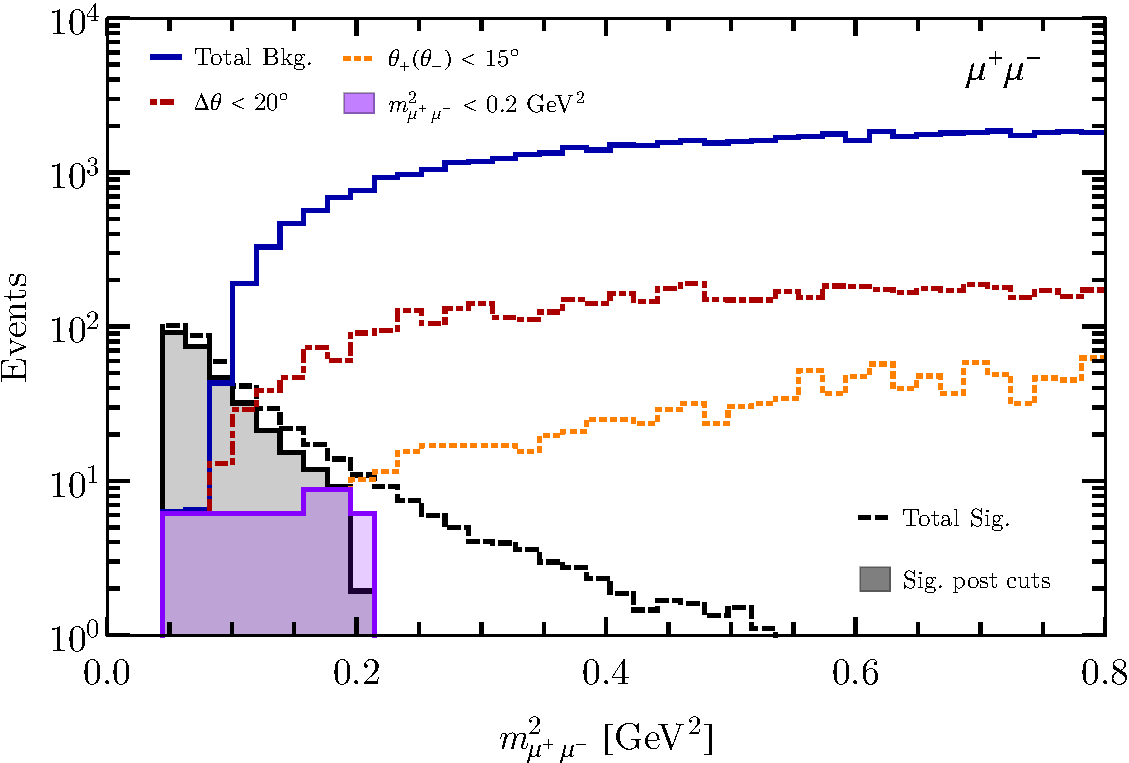
\includegraphics[width = 0.75\textwidth]{figs/SigvsBkg.pdf}
 \caption[Kinematical cuts on background samples for dimuon tridents.]{Signal and background distributions in invariant mass. The total background events (blue) include the misID rates in table \reftab{tab:misIDlist}. We apply consecutive cuts on the background, starting with cuts on the separation angle $\Delta \theta$ (red), both charged lepton angles to the beamline ($\theta_+$ and $\theta_-$) (orange) and the invariant mass $m^2_{\mu^+ \mu^-}$ . We show the signal samples before and after all the cuts in dashed black and filled black, respectively. \label{fig:bkg_flow}}
\end{figure}
%
Finally, we comment on some of the limitations of our analysis. The low rate of trident events calls for a more careful evaluation of other subdominant processes that could be easily be overlooked. For channels involving electrons, it is possible that de-excitation photons and internal bremsstrahlung become a source of background, as these also produce very soft EM showers, none of which are implemented in GENIE. The question of reconstruction of these soft EM showers, accompanied either by a high energy muon or by another soft EM shower also would have to be addressed, especially in the latter case where a trigger for these soft events would have to be in place. A more complete analysis is also needed for treating the decay products of charged pions and muons produced in neutrino interactions, as well as rare meson decay channels (like the Dalitz decay of neutral pions $\pi^0 \to \gamma e^+ e^-$). Cosmic ray events are not expected to be a problem due to the requirement of a vertex and a correlation with the beam for trident events. Perhaps even more exotic processes, such as the production of three final-state charged leptons ($\nu_{\alpha} (\overline{\nu}_{\alpha}) + \mathcal{H} \to  \ell_\alpha^- (\ell_\alpha^+) + \ell_\beta^+ + \ell_{\beta}^- + \mathcal{H^\prime}$), can also become relevant. For instance, radiative trimuon production \cite{Smith:1977nx} can potentially serve as a background to dimuon tridents if one of the muons is undetected. Similarly, $\mu e e$ production would fake a dielectron (mixed) trident signature if the muon (an electron) is missed. We are not aware of any estimates for the rate of these processes at the DUNE ND, but we note that their rate can be comparable to trident production at energies above $30$ GeV \cite{Albright:1978mg}. Improvements on our analysis should come from the collaboration's sophisticated simulations, allowing for a better quantification of hadronic activity, more realistic misID rates and more accurate detector responses.  

%%%%%%%%%%%%%%%%%%%%%%%%%%%%%%%%%%%%%%%%%%%%%%%%%%%%
\section{Conclusions}

\label{sec:conc}
Neutrino trident events are predicted by the SM, however, only $\overline{\nu}_\mu$ initiated dimuon tridents have been observed in small numbers, typically fewer than 100 events. This will change in the near future thanks to the current and future generations of precision neutrino scattering and oscillation experiments, which incorporate state-of-the-art detectors located at short distances from intense neutrino sources. 
%
In this work we discuss the calculation of the neutrino trident cross section for all flavours and hadronic targets, and provide estimates for the number and distributions of events at 9 current or future neutrino detectors: five detectors based on the new LAr technology (SBND, $\mu$BooNE, ICARUS, DUNE ND and $\nu$STORM ND) as well as four more conventional detectors (INGRID, MINOS ND, NO$\nu$A ND and MINER$\nu$A). The search for tridents, however, need not be exclusive to near detectors of accelerator neutrino experiments. As pointed out by the authors of Ref.~\cite{Ge2017}, atmospheric neutrino experiments can also look for these processes, benefiting from the increase of the cross section at large energies. 

We have stressed the need for a full four-body phase space calculation of the trident cross sections without using the EPA. This approximation has been employed in recent calculations and can lead to overestimations of the cross section by 200\% or more at the peak neutrino energies relevant for many accelerator neutrino experiments.
%
Moreover, we show why the EPA is not applicable for computing trident cross sections, and provide the first quantitative assessment of this breakdown for coherent and incoherent hadronic regimes. 
%
We find that the breakdown of the approximation is most severe for processes with electrons in the final-state and for incoherent scattering of all final state flavours. 
%
For coherent dimuon production, the approximation can give a reasonable result at large neutrino energies. This is due to the nuclear form factors that serendipitously suppress those regions of phase space where the EPA is least applicable. We also demonstrated that the best results in this channel are achieved when applying artificial cuts to the phase space.
%
However, even in this case, at energies relevant for the above experiments, the EPA can artificially suppress the coherent scattering contribution and increase the incoherent one giving rise to an incorrect rate and distributions of observable quantities. 
%
For instance, the invariant mass of the charged lepton pair $m^2_{\ell \ell}$ and their angular separation $\Delta \theta$ are more uniformly distributed for incoherent than for coherent trident scattering. Using the correct distributions is crucial to correctly disentangle the signal from the background by cutting on these powerful discriminators.

Our calculations show that DUNE ND is the future detector with the highest neutrino trident statistics, more than 6000 mixed events, 11\% produced by incoherent scattering, more than 1900 dielectron events, 5\%  produced by incoherent scattering and about 750 dimuon events,
almost 34\% of those produced by a incoherent process. Making use of our efficiencies (see \reftab{tab:DUNE_ND_NU_BG}), assuming an ideal background suppression and neglecting systematic uncertainties, we quote the statistical uncertainty on the coherent-like flux averaged cross section for the DUNE ND. We do this for coherent only events and, in brackets, for coherent plus incoherent events, yielding
%
\[\frac{\delta \langle \sigma^{e^\pm\mu^\mp} \rangle}{\langle \sigma^{e^\pm\mu^\mp} \rangle} =  1.8\% \, (1.6\%), \quad \frac{\delta \langle \sigma^{e^+e^-} \rangle}{\langle \sigma^{e^+e^-} \rangle} =  3.4\% \,(3.3\%) \quad \mathrm{and} \quad \frac{\delta \langle\sigma^{\mu^+\mu^-} \rangle}{\langle \sigma^{\mu^+\mu^-} \rangle} =  5.5\% \,(5.1\%).\]
%
In this optimistic framework we expect the true statistical uncertainty on coherent-like tridents to lie between the two numbers quoted, depending on how many incoherent events contribute to the coherent-like event sample. This impressive precision would provide unprecedented knowledge of the trident process and the nuclear effects governing the interplay between coherent and incoherent regimes. We emphasize, however, that given these small values for the relative uncertainties, the trident cross section will likely be dominated by systematic uncertainties from detector response and backgrounds which are not modelled here. 

For DUNE ND, we have studied the distribution of observables which could help distinguish trident events from the background. We have estimated the background for each trident channel via a Monte Carlo simulation using GENIE, and identified the dominant contributions arising primarily from particle misidentification.  
%
We conclude that reaching background rates of the order 
${\cal O}(10^{-6}-10^{-5})$ times the CC rate is necessary to observe trident events at DUNE ND, and given the distinctive kinematic behaviour of the trident signal a simple cut-based GENIE-level analysis suggests that this is an attainable goal in a LAr TPC. 

Existing facilities may also be able to make a neutrino trident measurement at their near detectors. Despite not including reconstruction efficiencies nor an indication of the impact of backgrounds, we find that the largest trident statistics is available at INGRID, the T2K on-axis near detector. We predict about 660 (1700) events for the mixed flavour, 300 (770) events for the dielectron and 50 (130) events for the dimuon channel for T2K-I (T2K-II). The more fine-grained near detector of MINOS and MINOS+ is also expected to have collected a significant numbers of events during its run. As such, the very first measurement of neutrino trident production of mixed and dielectron channels may be at hand.


%%%%%%%%%%%%%%%%%%%%%%%%%%%%%%%%
\section{Individual Backgrounds}
\label{app:backgrounds}
Here we discuss backgrounds to trident final-states in more detail. We start by motivating our misID rates shown in \reftab{tab:misIDlist}, and then discuss the dominant background processes individually.

In LAr photons can be distinguished from a single electron if their showers start displaced from the vertex (if present). Photons have a conversion length in LAr of around 18 cm, meaning $5$--$10\%$ could be expected to convert quickly enough to hinder electron-photon discrimination by this means if the resolution on the gap is from $1$--$2$ cm \cite{Acciarri:2016sli}. Once pair conversion happens, photons can be distinguished from a single electron purely by $\dd E/\dd x$ measurements in the first 1--2 cm of their showers. Motivated by the success of this method as shown at ArgoNeuT \cite{Acciarri:2016sli} and based on projections for DUNE \cite{Acciarri:2016ooe}, we assume that $5\%$ of photons would be taken as $e^\pm$ with perfect efficiency, without the need for an event vertex. Needless to say that a dedicated study for trident topologies would be necessary for a more complete study. It is worth noting that our remarks concern only the misID of a single photon for a single electron, whilst the distinction between a photon and an overlapping $e^+e^-$ pair without a vertex can be much more challenging. For this reason we take the misID rate between an overlapping $e^+e^-$ pair and a photon to be 1 in the absence of a vertex.  

Charged pions are notorious for faking long muon tracks. We estimate this misID rate as arising from through-going pions, which do not exhibit the decay kink used in their identification. We assume an interaction length of around $1$ m, meaning that about $5\%$ of particles travel $\sim3$ meters and escape the fiducial volume. Assuming that this is the most likely way a pion can spoof a muon, we estimate a naive suppression rate of $10^{-2}$. In a more complete study, it is desirable to explore the length of the muon and pion tracks inside the detector as a function of energy. The length of the contained tracks can also be an important tool for background suppression which we leave to future studies.  

%%%%%%%%%%%%%%%%%%%%%%%%%%%%%%%%%%%%%%%%%%%%%%%%%%%%
\subsection{Pion Production}

Coherent pion production in its charged ($\nu + A \to \ell^\mp + \pi^\pm + A$) and neutral ($\nu + A \to \nu + \pi^0 + A$) current version is very abundant at GeV energies. The cross section for these processes is modelled in GENIE using a modern version of the Rein-Sehgal model \cite{REIN198329,Rein:2006di}. The charged current version serves mainly as a background to $\mu^+ \mu^-$ tridents, but can also appear as a background for $e^\pm \mu^\mp$ tridents for incoming electron neutrinos or antineutrinos. It has been studied before at MiniBooNE \cite{AguilarArevalo:2010xt}, MINER$\nu$A \cite{Higuera:2014azj,Mislivec:2017qfz}, T2K \cite{Abe:2016fic,Abe:2016aoo}, and for the first time in LAr at ArgoNeuT \cite{Acciarri:2014eit}. This process has a very distict low 4-momentum transfer to the nucleus $|t|$ \cite{Higuera:2014azj}, but a much flatter distribution in invariant mass if compared to trident. The neutral current version of coherent pion production serves as a background to $e^+e^-$ tridents. This process has been studied before by the MiniBooNE \cite{AguilarArevalo:2009ww}, SciBooNE \cite{Kurimoto:2010rc} and in LAr by the ArgoNeuT collaboration \cite{Acciarri:2015ncl}. There are two possibilities for these events to fake an $e^+e^-$ trident: when one of the gammas produced in the $\pi^0$ decay is missed and the other is misIDed for an overlapping $e^+e^-$ pair, and when both photons are each misIDed for a single electron. This signature also comes with low hadronic activity, but for separated visible photons the invariant mass is a natural discriminator, as in the detector $m_{\gamma \gamma} \approx m_{\pi^0}$.

Resonant pion production can also contribute to trident backgrounds in the absence of any reconstructed protons. Resonant pion production can be larger than its coherent counterpart and is modelled in GENIE by the Rein-Sehgal model \cite{Rein:1980wg}. Its CC version was measured by MiniBooNE \cite{AguilarArevalo:2010xt}, K2K \cite{Mariani:2010ez}, MINOS \cite{Adamson:2014pgc}, and MINER$\nu$A \cite{Altinok:2017xua}. In the latter measurement one can clearly see the large number of events with undetected protons. The misIDed photon and the charged lepton invariant mass are once more flatter than the trident ones, allowing for a kinematical discrimination whenever a single photon is undetected. It is worth noting that these are some of the dominant underlying processes for pion production in GENIE, but all events leading to topologies relevant for trident are included in our analysis.
%
%%%%%%%%%%%%%%%%%%%%%%%%%%%%%%%%%%%%%%%%%%%%%%%%%%%%
\subsection{Charm Production}

Since the first observation of dimuon pairs from charm production in neutrino interaction by the HPWF experiment in 1974 \cite{Benvenuti:1975ru}, a lot has been learned about these processes (see \cite{Lellis:2004yn} for a review) in neutrino experiments. Particularly, the production of charm quarks and their subsequent weak decays into muons or electrons have been identified as a major source of background for early trident searches. At the lower neutrino energies at DUNE, however, this is expected to be a smaller yet non-negligible contribution. From our GENIE samples, we estimate that a charmed state is produced at a rate of around $10^{-4}(N_\text{CC}+N_\text{NC})$. Most of these produce either D mesons, 
$\Lambda_c$ or $\Sigma_c$ baryons. These particles decay in chains, emitting a muon with a branching ratio of around $0.1$, and are always accompanied by pions or other hadronic particles. We therefore expect these rates to be negligible with a hadronic veto, and do not consider them further. We hope, however, that future studies will address these channels in more detail.

%%%%%%%%%%%%%%%%%%%%%%%%%%%%%%%%%%%%%%%%%%%%%%%%%%%%
\subsection{CC$\gamma$ and NC$\gamma$}

The emission of a single photon alongside a CC process could be a background for $\mu e$ tridents if the photon is misIDed as a single electron. When the photon is produced in a NC event, it can be a background to overlapping $e^+e^-$ tridents. In GENIE, these topologies arise mainly due to resonance radiative decays and from the intra-nuclear processes. For this reason, it usually comes accompanied with extra hadronic activity. For hadronic resonances, we have simulated CC processes in GENIE and estimated
the multiplicities: $0.5\%$ single
photon and $1\%$ double photon emission from CC rates. Radiative photon production from the charged lepton, on the other hand, does not need to come accompanied by hadrons. It is phase space and $\alpha\approx1/137$ suppressed with respect to CCQE rates, and therefore could occur at appreciable rates compared to our signal. This contribution, however, is not included in GENIE and is absent from our samples. The rates of internal photon bremsstrahlung have been estimated before, particularly for T2K where a low-energy photon is an important background for electron
appearance searches \cite{Efrosinin:2009zz}, and as a background to the low energy events at MiniBooNE \cite{Bodek:2007wb}. De-excitation gammas from the struck nuclei can also generate CC$\gamma$ or NC$\gamma$ topologies \cite{PhysRevLett.108.052505}. These contributions for Ar are not included in GENIE, but are expected to come with a distinct energy profile, which can be tagged on.

%%%%%%%%%%%%%%%%%%%%%%%%%%%%%%%%%%%%%%%%%%%%


\chapter{New fundamental forces at DUNE}
\graphicspath{{}{Zprime_scattering/}}

\section{Introduction}

The discovery of neutrino oscillation is the first laboratory-based proof of physics Beyond the Standard Model (BSM) establishing that, in contrast to the predictions of the Standard Model (SM), the neutrino sector has at least three mass eigenstates distinct from the flavour states defined by the charged-leptons. However, the mechanism which generates neutrino masses remains unknown and many competing candidate theories exist, ranging from the simplicity of a Dirac mass term protected by a symmetry (see \eg\ \cite{Chulia:2016ngi,Ma:2014qra,Aranda:2013gga}) or the popular see-saw mechanisms \cite{Minkowski:1977sc,Mohapatra:1979ia,GellMann:1980vs,Yanagida:1979as,Lazarides:1980nt,Mohapatra:1980yp,Schechter:1980gr,Cheng:1980qt,Foot:1988aq} to proposals with a more elaborate spectrum of particles. In general, more elaborate scenarios have additional motivations, including the explanation of lepton mass and flavour hierarchies (see \eg\ \cite{King:2013eh}), the matter-antimatter asymmetry of the universe \cite{Fukugita:1986hr, Asaka:2005pn, Asaka:2005an}, the existence of dark matter \cite{Boehm:2006mi,Ma:2006km}, the scale of neutrino masses \cite{Gabriel:2006ns,Davidson:2009ha,Bertuzzo:2017sbj} or anomalous experimental results \cite{Nath:2016mts}. Uncovering the nature of new physics in the neutrino sector, and its connection to other BSM concerns, will be a central aim of the experimental and theoretical programs over the next few decades.

Although significant progress has already been made, the neutrino sector remains relatively poorly explored. There are still large uncertainties on the masses and on some of the mixing parameters of the light neutrinos \cite{Esteban:2018azc}, but even beyond the effects of neutrino mass, many SM cross sections are poorly known theoretically and infrequently measured. This is in part due to the typical energy scales of neutrino experiments which necessitate the mo\-del\-ling of the neutrino-nucleus interactions, but also because of the rareness of neutrino scattering (see \refref{Conrad:1997ne}). Much effort has gone into measuring crucial cross sections at oscillation experiments \cite{Abe:2015biq,Adamson:2009ju,Aguilar-Arevalo:2013dva} and at the Main Injector Experiment for $\nu$-A (MINER$\nu$A) \cite{Ren:2017xov}, a dedicated cross section experiment. However, given the necessity and potential richness of BSM physics in the neutrino sector, and the wide array of measurements yet to be made, it is conceivable that new physics will also manifest itself as detectable signatures in neutrino scattering. It is crucial to keep an open mind about what future experimental work might find, for instance, in the auxiliary physics program of the Near Detector (ND) of the next-generation Deep Underground Neutrino Experiment (DUNE) \cite{Acciarri:2016crz}.

Novel interactions in the neutrino sector have been proposed for a variety of reasons, including as a potentially observable effect in the neutrino oscillation probabilities (see \eg\ \cite{Blennow:2016jkn}), as a way of ameliorating tension introduced by sterile neutrinos in the early universe~\cite{Hannestad:2013ana, Dasgupta:2013zpn,Mirizzi:2014ama,Cherry:2016jol,Capozzi:2017auw,Denton:2018dqq,Chu:2018gxk,Esmaili:2018qzu}, and as a possible explanation of anomalous results at short baseline~\cite{Bertuzzo:2018itn,Ballett:2018ynz,Arguelles:2018mtc}. Models which introduce new interactions between neutrinos and matter have been discussed in simplified settings~\cite{Boehm:2004uq, Cerdeno:2016sfi,Denton:2018xmq}, via Effective Field Theory \cite{Falkowski:2018dmy,Falkowski:2019xoe} and specific UV complete models~\cite{Farzan:2015doa} (see also \cite{Bakhti:2018avv} for a neutrinophilic $Z^\prime$ study at the DUNE ND).
%
One class of models restricts the new interactions to leptons. This arises most naturally in settings with a gauged subgroup of lepton number, with most attention given to the anomaly free subgroups $L_\alpha - L_\beta$ for $\alpha,\beta \in \{e,\mu,\tau\}$ \cite{He:1991qd,He:1990pn}. Such leptophilic interactions must satisfy strong constraints from processes involving charged-leptons \cite{Bauer:2018onh}, but in the case of a gauged $L_\mu - L_\tau$ symmetry, neutrino processes have been found to be particularly competitive \cite{Altmannshofer2014}.

In this work, we study potential constraints which can be placed on a general set of leptophilic $Z^\prime$ models in the two most likely scattering channels for this type of BSM at the near detector of DUNE: $\nu-e$ scattering and $\nu\ell\ell$ trident scattering. During ten years of running, a 75-t near detector subjected to the intense neutrino beam at the Long-Baseline Neutrino Facility (LBNF) will provide tens of thousands of $\nu-e$ scattering events. The cross section for this process is theoretically well understood and can therefore be a sensitive probe of BSM physics. Additionally, this process has received special interest due to its potential in reducing systematic uncertainties in the neutrino flux~\cite{Park:2013dax,Bian:2017axs}, an undertaking which can be affected by new physics. Despite not being a purely leptonic process, neutrino trident production can also be measured with reasonable precision at DUNE, where hundreds of coherent and diffractive trident events are expected at the ND~\cite{Ballett:2018uuc}. We study the neutral current channels with dielectron or dimuon final states, pointing out how the new physics contribution impacts the non-trivial kinematics of these processes. The main advantage in such measurements lies on the flavour structure of dimuon tridents, which can be used to constrain otherwise difficult to test models, such as the one where a new force is associated to the $L_\mu-L_\tau$ gauge symmetry~\cite{Altmannshofer2014}.

Although these processes can place stringent bounds on many classes of mediators, many scenarios are already heavily constrained through other experimental work. A recent study of several different $U(1)_X$ models using $\nu-e$ scattering was presented in Ref.~\cite{Lindner:2018kjo}, where data from past $\nu-e$ experiments CHARM-II, GEMMA and TEXONO has been used to put bounds on the couplings and masses of general $Z^\prime$s. Novel charged particles are typically constrained to be very massive, leading to little enhancement of the charged current neutrino scattering rates. In particular, charged scalars have been considered in $\nu\ell\ell$ trident scattering in \refref{Magill:2017mps}, where it is found that trident measurements can provide competitive bounds on charged scalars, albeit only in simplified theoretical settings. The requirement of doubly charged scalars or the connection to neutrino masses introduced by the typical UV completions of such models dilutes the relevance of the trident bounds. Neutral scalars are viable, but also present challenging UV completions. Novel $Z^\prime$ interactions in $\nu\ell\ell$ trident scattering with dimuon final states have been studied in \refref{Altmannshofer2014}, where it was shown to be a promising channel to probe a $L_\mu-L_\tau$ gauge symmetry. This model was revisited in \refrefs{Kaneta:2016uyt}{Araki:2017wyg}, where the effects of kinetic mixing and the possibility of a measurement by T2K was alluded to. Finally, neutrino trident scattering with atmospheric neutrinos was shown to be sensitive to this model as well as to simplified scalar models in \cite{Ge:2017poy}. It should be noted, however, that as it was shown in \refref{Ballett:2018uuc} the Equivalent Photon Approximation (EPA) discussed in several recent studies \cite{Magill:2017mps, Kaneta:2016uyt} for the calculation of the trident cross section leads to intolerably large errors in the predictions for the $\nu\ell\ell$ scattering channels in the SM. For this reason, we calculate this process without making this approximation.

The structure of the paper is as follows. In \refsec{sec:models}, we describe the basic properties of the leptophilic scenarios that we will consider in this work. In \refsec{sec:signatures}, we discuss the calculation of the trident and $\nu-e$ scattering cross sections in a general model of leptophilic $Z^\prime$. In \refsec{sec:sensitivities}, we show how DUNE can place bounds on a few popular leptophilic $Z^\prime$ models, discussing our assumptions for experimental configurations and backgrounds. We make our concluding remarks in \refsec{sec:conclusion}.

%%%%%%%%%%%%%%%%%%%%%%%%%%%%%%%%
\section{\label{sec:models}Leptophilic $Z^\prime$ models}

Since we are interested in models where the novel neutral currents are present only in the lepton sector, let us consider explicitly a ${\rm U(1)}_{Z^\prime}$ extension of the SM whose Lagrangian is given by
%
\begin{equation}\label{eq:lagrangian}
\mathcal{L} \supset -g^\prime Z^\prime_\mu \left[ Q^\text{L}_\alpha\, \overline{L_L^\alpha}\gamma^\mu L_L^\alpha  + Q^\text{R}_\alpha\, \overline{\ell_R^\alpha}\gamma^\mu \ell_R^\alpha + \sum_{\rm N} Q_\text{N}\, \overline{N_R}\gamma^\mu N_R \right],
\end{equation}
%
where $L_\alpha$ ($\ell_\alpha$) represents the leptonic SU(2) doublet (singlet) of flavour $\alpha\in\{e,\mu,\tau\}$, and we included ${\rm N}$ right-handed neutrinos with charges $Q_{\rm N}$ under the new symmetry for completeness. Thus, we have $7+{\rm N}$ new parameters to characterize the couplings between the new boson and the lepton sector, one gauge coupling $g^\prime$ and $6+N$ charges $\{Q_\alpha^\text{L}, Q_\alpha^\text{R}, Q_\text{N}\}$. Below the scale of the Electroweak Symmetry Breaking (EWSB), the relevant interaction terms in the Lagrangian are given by 
%
\begin{align}\label{eq:lagrangian_below_EWSB}
\mathcal{L} \supset &-g^\prime Z^\prime_\mu \big[ Q^\text{L}_\alpha\,\overline{\nu_\alpha}\gamma^\mu P_\text{L}\nu_\alpha  + \frac{1}{2}\,\overline{\ell_\alpha}\gamma^\mu(Q_\alpha^\text{V} - Q_\alpha^\text{A}\gamma^5) \ell_\alpha \nonumber\\ &\quad\quad\quad\quad+ \sum_{\rm N} Q_\text{N}\, \overline{N_R}\gamma^\mu N_R \big],
\end{align}
%
where $Q^\text{V}_\alpha \equiv Q^\text{L}_\alpha + Q^\text{R}_\alpha$ and $Q^\text{A}_\alpha \equiv Q^\text{L}_\alpha - Q^\text{R}_\alpha$. We note that the right-handed singlets could modify the form of the neutrino interaction in \refeq{eq:lagrangian_below_EWSB} by introducing a right-chiral current. The details of this would depend on the relationship between these chiral states and the flavour-basis neutrino $\nu_\alpha$. However, in practice our Lagrangian is fully general, as the polarization effects in the neutrino beam ensure that only the left-handed charge is relevant for light-neutrino scattering experiments. 

The Lagrangian in \refeq{eq:lagrangian} contains all of the terms necessary for this analysis. However, when it comes to assigning specific charges to the particles, a few wider model-building considerations are worthy of discussion. In the SM, any non-vectorial symmetry would forbid the Yukawas responsible for the charged-lepton mass terms post-ESWB; similarly, possible negative implications for neutrino mass generation are expected. The precise implementation of the neutrino mass mechanism is highly model dependent, but neutrino gauge charges are not compatible with many usual realizations\footnote{If neutrino masses are thought of as coming from a Weinberg operator, it is clear that the leptonic doublet must be uncharged under any unbroken U$(1)^\prime$ group.}. Furthermore, the novel gauge boson $Z^\prime$ will also require a mass generation mechanism, and indeed this could be achieved via the means of symmetry breaking. Although each of these is an important aspect of model building, their resolution can be expected to have little impact on the phenomenology of neutrino scattering, and we will not pursue them here.
%
Anomaly freedom of our new symmetry, however, is a more pertinent concern. It has been shown that an anomalous group can always be made anomaly free via the introduction of exotically charged sets of fermions which can be given arbitrarily large masses \cite{Batra:2005rh}. Yet these novel fermionic states necessarily introduce effects at low-scales, which in some cases can strongly affect the phenomenology of the model \cite{Dror:2017ehi}. Therefore, while it seems likely that mass generation can be addressed with the addition of new particles which do not interfere with neutrino scattering phenomenology, anomaly freedom is more pernicious. For this reason we will briefly discuss how anomaly freedom will dictate the types of leptonic symmetries that we consider in the remainder of this work.

\paragraph{Anomaly freedom.} The most general anomaly-free symmetries compatible with the SM were first deduced in the context of Grand Unification Theories (GUT) \cite{Barger:1982bj,Barr:1986hj}. More recently, an atlas of all anomaly-free $U(1)$ extensions of the SM with flavour-dependent charges has been provided by Ref.~\cite{Allanach:2018vjg}. Interestingly, the only anomaly-free subgroups of the SM with renormalisable Yukawa sector are leptophilic: the lepton-family number differences $L_\alpha -L_\beta$ $(\alpha,\beta=e,\mu,\tau)$ \cite{He:1990pn,He:1991qd}. The popular $B-L$ symmetry is in fact anomalous unless right-handed SM singlets are added with the appropriate charges. This is well motivated by the necessity of neutrino mass ge\-ne\-ra\-tion but remains a hypothesis, as not all models of neutrino mass require novel fermionic content. 
%
For the sake of discussion, we follow a similar logic and consider the most general anomaly free subgroups of the SM accidental leptonic symmetries allowing for an arbitrary number of right-handed fermionic singlets. These would presumably be associated with the neutrino mass generation mechanism, but we impose no specific relations in this regard due to the significant model-building freedom. The anomaly conditions for a leptophilic model with right-handed neutrinos are given below \cite{Ellis:2017nrp} \footnote{Notice that $\rm U(1)_{Z^\prime}^3$ together with gauge-gravity conditions imply that the number of right-handed states must be at least $N=3$.}
%
\begin{subequations}\label{eq:anom}
    \begin{align}
        {\rm SU(2)_W^2\times \rm U(1)_{Z^\prime}} & \quad\sum_\alpha Q_\alpha^{\rm L} = 0,\\
        {\rm U(1)_Y^2\times \rm U(1)_{Z^\prime}}& \quad\sum_\alpha\left[ \frac{1}{2}Q_\alpha^{\rm L} - Q_\alpha^{\rm R}\right]= 0,\\
        {\rm U(1)_Y\times \rm U(1)_{Z^\prime}^2} &  \quad\sum_\alpha \left[(Q_\alpha^{\rm L})^2 - (Q_\alpha^{\rm R})^2\right]= 0,\label{eq:YZp2}\\
        {\rm U(1)_{Z^\prime}^3} & \quad \sum_\alpha  \left[2 (Q_\alpha^{\rm L})^3 - (Q_\alpha^{\rm R})^3\right] - \sum_{\rm N}Q_{\rm N}^3= 0,\\
        \text{Gauge-Gravity} & \quad \sum_\alpha \left[2Q_\alpha^{\rm L} - Q_\alpha^{\rm R}\right] - \sum_{\rm N} Q_{\rm N} = 0.
    \end{align}
\end{subequations}
%

In the absence of new $N_R$ particles ($Q_{\rm N}=0$) and assuming that $Q_{\alpha}^{\rm L}=Q_{\alpha}^{\rm R}$, that is considering vector couplings, we find the three well-known discrete solutions for the Eqs.~\eqref{eq:anom}: the antisymmetric pairs $L_\alpha- L_\beta$, $\alpha,\beta = \{e,\mu,\tau\},\ \alpha\neq\beta$. As far as anomalies are concerned, all three pairs are equal, but frequently focus falls on $L_\mu-L_\tau$, which has no coupling to electrons and correspondingly weaker constraints. If we reconsider these conditions with charged right-handed neutrinos, we find a one dimensional continuous family of potential symmetries which can be consistently gauged. We can parametrise this as
%
\begin{align}
     \varrho (L_\alpha - L_\beta) + \vartheta (L_\beta - L_\lambda),
\end{align}
%
with
\begin{align}\label{eq:Ncharges}
3\varrho\,\vartheta(\vartheta - \varrho) = \sum_{\rm N}Q_{\rm N}^3. 
\end{align}
What we have shown is that linear combinations of the $(L_\alpha - L_\beta)$ choice of charges yield an anomaly free scenario provided N right-handed neutrinos respecting \refeq{eq:Ncharges} are added to the theory. We have checked that the ``anomaly-free atlas'' in~\cite{b_c_allanach_2018_1478085} contains a subset of these solutions, which are more general.

The above conclusions are based on the assumption of vectorial charge assignments. In the SM, this requirement is a consequence of the origin of mass assuming a chargeless Higgs. However, in non-minimal models this requirement could be relaxed. Even with this extra freedom, not all charge assignments are allowed: for example, a purely chiral $U(1)^\prime$ cannot satisfy \refeq{eq:YZp2} without additional matter charged under the SM gauge group. The axial-vector case, however, does have further solutions: we find that the same one-dimensional family of charges is allowed as for the vectorial gauge boson --- in this case, the charges apply to the left-handed fields and the right-handed ones have the opposite charges. In such a model the leptonic mass generation mechanism would necessarily be more complicated than in the SM, but such a possibility is not excluded. UV completions of an axial-vector $Z^\prime$ have been presented in \cite{Ismail:2016tod,Kahn:2016vjr}, however, these generally introduce extra bounds that are expected to be stronger than neutrino scattering bounds (see \eg\ \cite{Dror:2017nsg,Dror:2017ehi}). For this reason, we only comment on the consequences of an axial-vector case in our calculations, but do not develop any particular model or constraint.


\paragraph{Kinetic mixing.} The symmetries of our SM extensions allow for kinetic mixing between the $Z^\prime$ and the SM gauge bosons \cite{Holdom:1985ag,Kamada:2015era,Ibe:2016dir}
%
\begin{align}
    \mathcal{L}_{\rm mix} = -\frac{\varepsilon}{2}F_{\kappa \rho}F^{\prime\,\kappa\rho},
\end{align}
%
where $F_{\kappa \rho}$ and $F^{\prime\,\kappa \rho}$ are the field strength tensors of the hypercharge and the $Z^\prime$ boson, respectively. The presence of such coupling introduces a very rich phenomenology and has been explored in great detail in the literature \cite{Alexander:2016aln}. In this work, we choose to focus on the less constrained possibility of vanishing tree-level kinetic mixing. In this case, kinetic mixing is still radiatively generated due to the presence of particles charged under both the SM and the new $U(1)$ group. As well as the SM particle content, additional particles present in the UV theory may also contribute to kinetic mixing, but we will neglect these contributions in this study as they are highly model dependent \footnote{The authors of Ref.~\cite{Escudero:2019gzq} have calculated the contribution to kinetic mixing in the $L_\mu-L_\tau$ model from a pair of scalars with opposite charges. These are typically subdominant, provided the mass hierarchy between the two scalars is not much larger than that of the charged leptons.}. We compute $\varepsilon$ between the $Z^\prime$ and the SM \emph{photon}, and find the one-loop result to be finite for any $\varrho(L_\alpha - L_\beta) + \vartheta (L_\beta - L_\lambda)$ gauge group, with divergences cancelling between families. In particular, for the $L_\mu-L_\tau$ model our result is in agreement with Refs.~\cite{Araki:2017wyg,Escudero:2019gzq}
\begin{align}
    \varepsilon(q^2) = &\frac{e g^\prime}{2\pi^2} \int_{0}^{1}\dd x\, x (1-x) \ln{\frac{m_\mu^2 - x(1-x)q^2}{m_\tau^2 - x(1-x)q^2}} \nonumber \\ &\quad\xrightarrow{q^2 \to 0} \,\, \frac{e g^\prime}{12 \pi^2} \ln{\frac{m_\mu^2}{m_\tau^2}}.
\end{align}    
Note that the finiteness of the one-loop result has important consequences for the leptophilic theories we consider. As pointed out in \refref{Bauer:2018onh}, the finiteness of $\varepsilon$ implies that one is able to forbid tree-level kinetic mixing, albeit in a model dependent manner. This happens, for instance, when embedding the new leptophilic $U(1)$ group in a larger non-abelian group $G$, which is completely independent from the SM sector. This choice of one-loop generated kinetic mixing should be seen as a conservative choice; in the absence of cancellation between tree and loop-level kinetic mixing, this yields the least constrained scenario for an $L_\mu-L_\tau$ model. Additional constraints from first-family leptons are now relevant \cite{Kamada:2015era,Araki:2015mya}, especially $\nu-e$ scattering measurements, where the strength of the constraint makes up for the loop suppression in the coupling. For neutrino trident scattering, one can safely ignore loop-induced kinetic mixing contributions in the calculation since these are either smaller than the tree-level new physics contribution or yield very weak bounds compared to other processes. 

We emphasize that if accompanied by a consistent mechanism for the generation of the $Z^\prime$ mass terms and leptonic Yukawa terms, the models we consider constitute a UV complete extension of the SM. The treatment of such scenarios lies beyond the scope of this work, but we note that if their scalar sectors are light enough they can also yield rich phenomenology at low scales \cite{Heeck:2011wj}.

\section{\label{sec:signatures}Signatures of leptonic neutral currents}

When a neutrino impinges on a detector it has only two options for BSM scattering via a leptophilic mediator. In the simplest scenario, the neutrino interacts via the new mediator with the electrons of the detection medium. In this case, there is a tree-level $\nu-e$ scattering process which would be expected to show the clearest signs of new physics. For scattering off a hadron, however, the leptophilic nature of the mediator means that the first tree-level contribution will necessarily come from a diagram which also includes at least one additional SM mediator.
%
Any neutrino-hadron scattering process can be embellished with the new boson to create a BSM signature. In general, the final states of these processes will be either identical to the original un-embellished process (perhaps with missing energy) or it will have an extra pair of leptons in the final state. These neutrino trilepton production processes, which we will refer to as tridents for simplicity, can be subdivided into four types:
%
\begin{itemize}
%
\item $\ell \ell \ell$ trident: $\mathcal{H} + \nu_\alpha \to \mathcal{H}^\prime + \ell^-_\alpha + \ell^+_\beta + \ell^-_\beta$
%
\item $\nu \ell \ell$ trident: $\mathcal{H} + \nu_\alpha \to \mathcal{H} + \nu_\beta + \ell^+_\gamma + \ell^-_\delta$
%
\item $\nu \nu \ell$ trident: $\mathcal{H} + \nu_\alpha \to \mathcal{H}^\prime + \ell^-_\alpha + \nu_\beta + \overline{\nu}_\beta$
%
\item $\nu \nu \nu$ trident: $\mathcal{H} + \nu_\alpha \to \mathcal{H} + \nu_\alpha + \nu_\beta + \overline{\nu}_\beta$
%
\end{itemize}
%

We note that these processes all occur in the SM, and so the hunt for new physics will necessarily be competing against a background of genuine SM events. Moreover, for final states with missing energy in the form of neutrinos, isolating a BSM signal would necessarily rely on spectral measurements and other backgrounds have the potential to be large. In particular, the trident production of $\nu\nu\nu$ and $\nu\nu\ell$ will be seen as contributions to the neutral-current (NC) elastic and charged-current quasi-elastic (CCQE) processes, and we expect backgrounds to be insurmountable (see \eg\ Ref.~\cite{Kelly:2019wow} for new physics contributions to CCQE processes). The $\ell\ell\ell$ channels, on the other hand, are expected to have a much more manageable SM background. Trimuon production, for instance, has been measured in the past and provides a multitude of kinematical observables in the final state~\cite{Holder:1977gp,KayisTopaksu:2004ea}. The SM rate for this channel contains radiative photon diagrams as well as hadronic contributions~\cite{Benvenuti1977,Barish1977,Smith1978}, whilst for leptophilic neutral bosons, the dominant  contributions comes from a weak process with initial and final state radiation of a $Z^\prime$, making it a less sensitive probe of light new physics. Finally, the $\nu \ell \ell$ production, the most discussed trident signature in the literature, has already been observed in the dimuon channel~\cite{Geiregat:1990gz,Mishra:1991bv,Goncharov:2001qe}. This channel is by far the most important trident process for our study, as the leptonic subdiagrams contain only weak vertices in the SM.

\subsection{Neutrino trident scattering}

\begin{figure*}
    \centering
    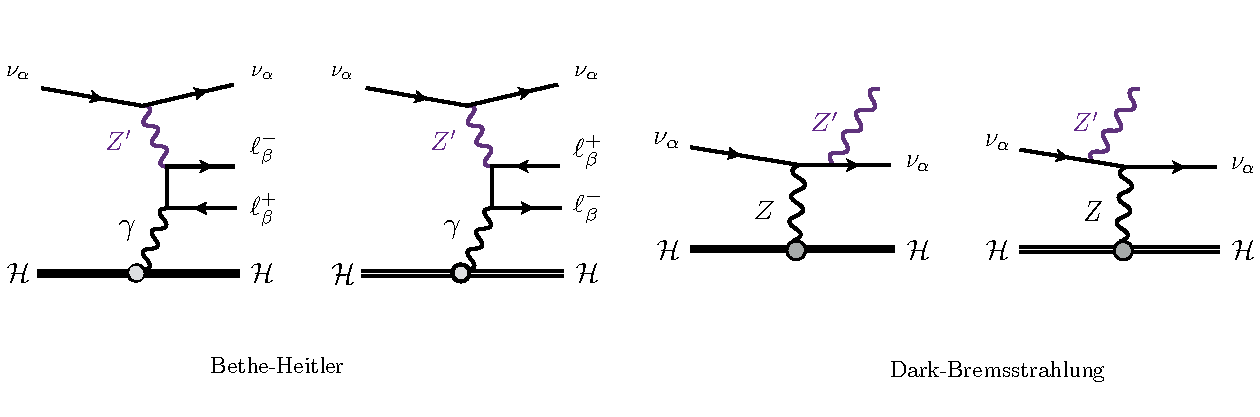
\includegraphics[width=0.94\textwidth]{tridentdiagrams.pdf}
\caption{The BSM contributions to neutrino trident production considered in our calculation. The diagrams on the left are referred to as Bether-Heitler contributions due to their resemblance to pair-production. On the right, we show diagrams with a radiative-like $Z^\prime$ emission, which allows for the production of on-shell $Z^\prime$ particles, which subsequently decays into a charged-lepton pair.\label{fig:trident_diagrams}}
\end{figure*}


In the $\nu \ell \ell$ neutrino trident scattering, an initial neutrino scatters off a hadronic target producing a pair of charged leptons in the process. Since we focus solely on neutral current processes and on flavour conserving new physics, no mixed flavour tridents are relevant and we can write 
%
\begin{align*} 
\mathcal{H} (P) + \nu_\alpha (p_1) \to \mathcal{H} (P^\prime) + \nu_\alpha (p_2)  + \ell^-_\beta (p_3) + \ell^+_\beta (p_4). 
\end{align*}
%
In the SM this process receives CC and NC contributions when $\alpha = \beta$, and is a purely NC process if $\alpha \neq \beta$. The BSM contributions to trident production we consider are shown in \reffig{fig:trident_diagrams}. Beyond computing the Bethe-Heitler (BH) contributions considered previously, we show that radiative contributions to these processes are generally small. Using the Narrow-Width-Approximation (NWA), we compute the cross section for the radiation of a $Z^\prime$ particle from a neutrino-nucleus interaction, which can then promptly decay to an $\ell^+\ell^-$ pair. We call these contributions Dark-Bremsstrahlung (DB) processes for their similarity with electron brehmsstrahlung in QED. We now discuss the two amplitudes individually.

\paragraph{Bethe-Heitler.} The BH amplitude can be written as follows 
%
\begin{equation}
\mathcal{M}_{\rm BH} = \frac{\mathrm{L}_\mu \,\mathrm{H}_{\rm EM}^{\mu}}{Q^2}\, ,
\end{equation}
%
where $Q^2 \equiv -q^2 = (P - P^\prime)^2$ is the momentum transfer and $\mathrm{H}_{\rm EM}^{\mu}$ the hadronic amplitude for coherent or diffractive electromagnetic scattering
%
\begin{align}
{\rm H}^\mu_{\rm EM} &\equiv \langle {\cal H}(P) \vert J_\mathrm{EM}^\nu (q^2)\vert {\cal H}(P^\prime)\rangle\,.
\label{eq:Hmu1}
\end{align}
%
We refer the reader to Ref. \cite{Ballett:2018uuc} for the details on the treatment of the hadronic amplitude. %our previous paper for the details on the treatment of the hadronic amplitude \cite{Ballett:2018uuc}. 
The leptonic amplitude for NC scattering $\mathrm{L}_\mu$ reads
%
\begin{align}
\mathrm{L}_\mu  \equiv - &\frac{ie G_F}{\sqrt{2}}[\bar{u}(p_2)\gamma^\tau(1-\gamma_5)u(p_1)] \nonumber\\
&\times 
\bar{u}(p_4)\Bigg[\gamma_\tau(\hat{V}_{\alpha\beta}-\hat{A}_{\alpha\beta}\gamma_5)\frac{1}{(\slashed{q}-\slashed{p}_3-m_3)}\gamma_\mu \nonumber \\ 
& + \gamma_\mu \frac{1}{(\slashed{p}_4-\slashed{q}-m_4)} \gamma_\tau (\hat{V}_{\alpha\beta}-\hat{A}_{\alpha\beta}\gamma_5) \Bigg] v(p_3)\,.
\label{eq:Lmu1}
\end{align}
%
In writing the equation above, we have introduced effective vector and axial couplings containing SM and BSM contributions
\begin{subequations}
\begin{align}
&\hat{V}_{\alpha \beta} = g^{\ell_{\beta}}_{V} + \delta_{\alpha \beta} +  \frac{Q_{\alpha}^L Q_{\beta}^V}{2\sqrt{2} G_{F}} \frac{(g^\prime)^2}{K^2 + M^2_{Z^\prime}},
\\&  
\hat{A}_{\alpha \beta} = g^{\ell_{\beta}}_{A} + \delta_{\alpha \beta} + \frac{Q_{\alpha}^L Q_{\beta}^A}{2\sqrt{2} G_{F}} \frac{(g^\prime)^2}{K^2 + M^2_{Z^\prime}}\,,
\label{eq:c_prescription_trident}
\end{align}
\end{subequations}

where $K^2 = -(p_1-p_2)^2$ and $g^{\ell_{\beta}}_{V}$'s $(g^{\ell_{\beta}}_{A}$'s) are the SM vector (axial) couplings. Note the dependence on the positive kinematic variable $K^2$ in the BSM contribution, which can lead to a significant peaked behaviour in the cross section. To avoid numerical difficulties, we have modified the phase space treatment proposed in \cite{Czyz1964,Lovseth1971}, as shown in \refapp{app:phase_space}. 


\paragraph{Dark-Bremsstrahlung.} Due to the small decay width of the $Z^\prime$ ($\Gamma \propto g^{\prime\,2} M_{Z^\prime}$), one can obtain an estimate for its resonant production using the NWA. In the true narrow-width limit, this process reduces to a 3-body phase space calculation and does not interfere with the BH amplitude \footnote{We note that despite the fact that interference terms between resonant and non-resonant contributions vanish in the narrow-width limit, the errors induced by the NWA can no longer be shown to be of the order of $\Gamma_{Z^\prime}/M_{Z^\prime}$ \cite{Uhlemann:2008pm}. Nevertheless, we do not expect a more careful evaluation of the resonant contribution to change our conclusions.}. Our DB amplitude
for $\nu_\alpha (k_a)\,+\,  {\rm A} (k_b) \to \nu_\alpha (k_1)\,+\, Z^\prime (k_2)\,+\, {\rm A} (k_3)$ reads 
%
\begin{equation}
    \mathcal{M}_{\rm DB} = g^\prime Q^L_{\alpha}\, \frac{G_F}{\sqrt{2}} \, J_\mu {\rm H}_{\rm W}^{\mu},
\end{equation}%
where ${\rm H}_{\rm W}^{\mu}$ is the weak hadronic current (see \refapp{app:formfactors}) and
\begin{align}
    J_\mu = &\overline{u}(k_1) \Big[ \gamma^\alpha \frac{\slashed{k_1}+\slashed{k_2}}{(k_1+k_2)^2} \gamma_\mu \nonumber \\ \quad&+ \gamma_\mu \frac{\slashed{k_a}-\slashed{k_2}}{(k_a-k_2)^2} \gamma^\alpha\Big] (1-\gamma^5) u(k_2) \, \epsilon^*_\alpha(k_2),
\end{align}
where $\epsilon^*_\alpha(k_2)$ is the polarization vector of the $Z^\prime$. The previous amplitude can then be squared and integrated over phase-space for the total DB cross section. The different charged lepton final states can then be imposed with their respective branching ratios (BR). As a final remark, we note that the typical decay lengths of the new boson are typically below 1 cm for the parameter space of interest, such that their decay is indeed prompt.

From the previous discussions it is clear that the contributions to the total cross section at the lowest order in $g^\prime$ 
come from the interference between the BSM and the SM BH diagrams, and from the DB. The latter, however, contains an extra power of $G_{\rm F}$ and is expected to be subdominant with respect to the BH interference. Our results for the individual flux integrated cross sections are shown in \reffig{fig:xsecs_mmmm} for the $\mu^+\mu^-$ and in \reffig{fig:xsecs_mmee} for the $e^+e^-$ trident channels. We show the BH contributions as well as the DB one normalized by the SM trident cross section. All cross sections are flux integrated using the $62.4$ GeV $p^+$ DUNE flux described in Section \ref{sec:experimental}. For generality, we do not include the BR factors in the DB contributions, and so the green lines only apply for $\mu^+\mu^-$ tridents if $M_{Z^\prime} > 2 m_\mu$ and would suffer additional suppression due to the BR. In each figure we show two panels, one for vector couplings and one for axial-vector couplings. This is interesting from a purely computational point of view, as it shows explicitly the BH cross section scaling with the $M_{Z^\prime}$ in the two cases. Whilst the scaling is similar for dielectron tridents, it differs significantly between the vector and axial-vector cases of the dimuon cross section. This suggests the presence of mass suppression effects in the BH process. We do not investigate this further, but note that there are large cancellations between the two BH diagrams in \reffig{fig:trident_diagrams} which are only present for vector-like couplings.

%
\begin{figure*}[t]
%
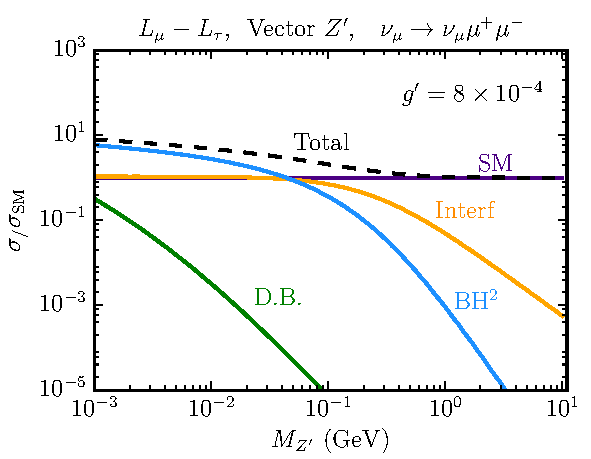
\includegraphics[width=0.43\textwidth]{SMvsBSMmass_xsec_mmmm_vec.pdf}
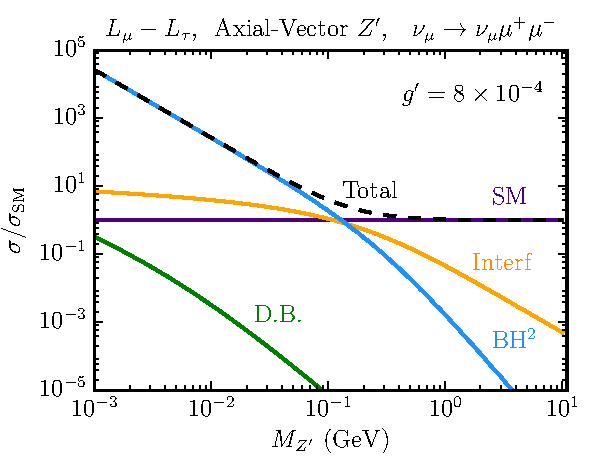
\includegraphics[width=0.43\textwidth]{SMvsBSMmass_xsec_mmmm_ax.pdf}
\caption{\label{fig:xsecs_mmmm} Flux integrated cross sections normalized to the flux integrated SM trident cross section for dimuon production. On the left (right) panel we show the vector (axial-vector) $Z'$ 
case. We separate the different contributions:
 SM only, interference between SM and BSM Bethe-Heitler contributions (interf) and BSM Bethe-Heither only (BH$^2$). The Dark-Bremsstrahlung (DB) cross section is also shown, but does not take the branching ratio into final state charged leptons into account.}
%
\end{figure*}
%
\begin{figure*}[t]
%
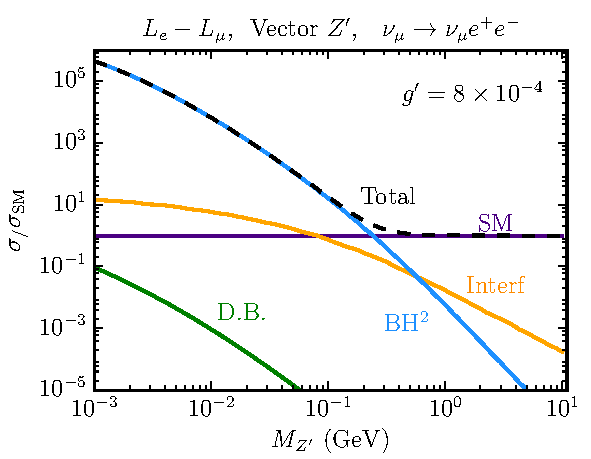
\includegraphics[width=0.43\textwidth]{SMvsBSMmass_xsec_mmee_vec.pdf}
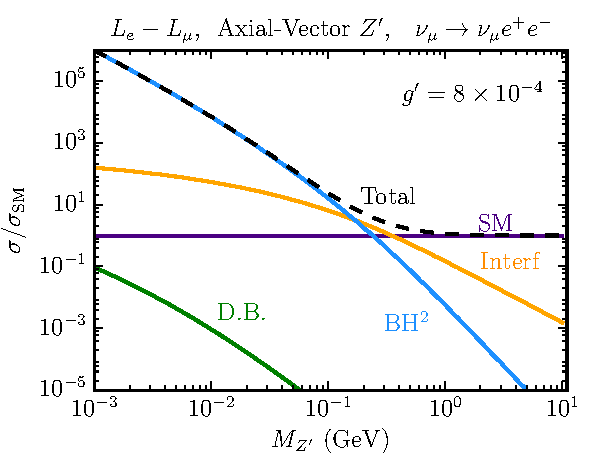
\includegraphics[width=0.43\textwidth]{SMvsBSMmass_xsec_mmee_ax.pdf}
%
\caption{\label{fig:xsecs_mmee} Same as \reffig{fig:xsecs_mmmm} but for the $e^+e^-$ trident channel.}
%
\end{figure*}

%
%%%%%%%%%%%%%%%%%%%%%%%%%%%%%%%%%%%%%%%%%%%%%%%%%%%%%%%%%%%%%%%%%%%%%%%%%%%%%%
\subsubsection{The Equivalent Photon Approximation \label{sec:EPA}}

We now comment on the EPA for neutrino trident production. This approximation is known to perform quite badly for the SM neutrino trident production cross section \cite{Ballett:2018uuc}. One may wonder, however, if the EPA gets better or worse when computing our BSM cross sections. Naturally, it would be most inadequate for the resonant-like cross sections, since the photon propagator and the strong $1/Q^4$ behaviour is absent. However, if one focuses on the BH contributions, a marginal improvement of the accuracy of the approximation is seen as one lowers the mass of the $Z^\prime$ mediator. In the SM, the $\nu-\gamma$ cross sections scale as a typical weak cross section, $\sigma_{\nu \gamma} \propto G_{\rm F}^2 \hat{s}$, where $\hat{s}$ is the square of the center of mass energy of the $\nu-\gamma$ system.  On the other hand, if the cross section is dominated by the BSM BH %Bethe-Heitler
contributions, %on the other hand, 
then as we take the limit of small $Z^\prime$ masses, it scales more similarly to a QED cross section, $\sigma_{\nu \gamma} \propto 1/\hat{s}$. This behaviour, however, is only present at low masses and only for the BSM contribution. Since we are interested in regions of the parameter space where BSM and SM cross sections are of similar size, then we expect the total cross section to have a behaviour which is a combination of the two. As a sanity check, we numerically verified that for parameter space points where the BSM contributions are of the same order as the SM cross section, the improvement in the accuracy of the EPA is still not satisfactory. For instance, the ratio between the EPA prediction and the full calculation for the dimuon channel assuming a $Q_{\rm max} = (140$ MeV$)/A^{1/3}$ goes from $\approx 30\%$ in the SM to $\approx 60\%$ for $g^\prime = 8\times10^{-4}$ and $M_{Z^\prime} = 5$ MeV. For this reason, we only use the full $2 \to 4$ calculation in what follows.

%%%%%%%%%%%%%%%%%%%%%%%%%%%%%%%%%%%%%%%%%%%%%%%%%%%%%%%%%%%%%%%%%%%%%%%%%%%%
\subsubsection{Trident kinematical distributions \label{sec:trident_kinematics}}
%
\begin{figure*}[t]
%
\centering
%
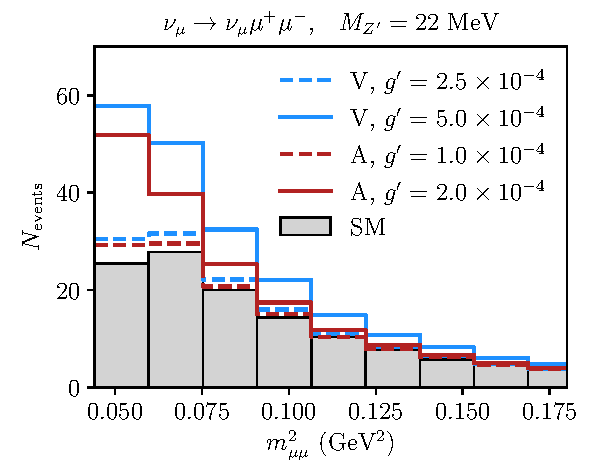
\includegraphics[width=0.4\textwidth]{BSM_invmass_mumu.pdf}
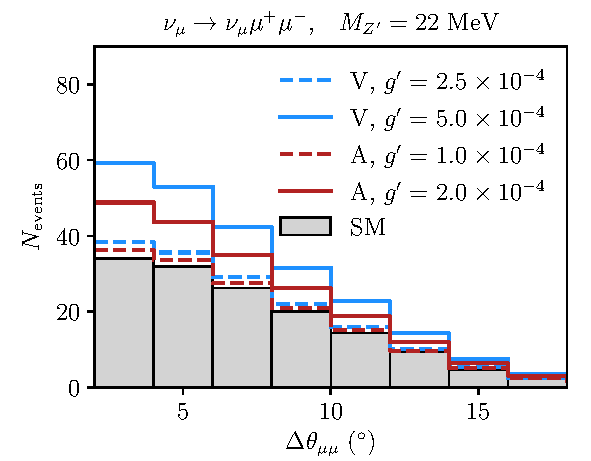
\includegraphics[width=0.4\textwidth]{BSM_sepangle_mumu.pdf}
%
\caption{
Distribution of the number of neutrino trident events as a function of the invariant mass of the dimuon pair (left) and their separation angle (right) at the DUNE ND. The distributions were produced using the DUNE 120 GeV $p^+$ neutrino beam and have been smeared as described in \refsec{sec:experimental}. For the new physics, we plot the case of a vector (V), $Q^L = Q^R$, and axial-vector (A), $Q^L = -Q^R$,  $Z^\prime$ assuming $Q^L_{\alpha}$ to be given by $L_\mu - L_\tau$. \label{fig:mm_spectra}}
\end{figure*}
%
The impact of new physics on the total cross section for trident production has been explored in the previous section. It is then natural to ask what the impact of new physics is on the kinematics of trident production which are, especially in the case of the invariant mass and angular variables, of utmost importance for background reduction. In this section we show how the new physics can alter the distributions of these important variables. All results that follow have been obtained using trident events produced by our dedicated Monte Carlo (MC). Smearing and selection cuts have been applied as detailed in Sec.~\ref{sec:sensitivities}.

The variables of interest in background reduction are the charged lepton invariant mass $m^2_{\ell \ell}$ and their separation angle $\Delta \theta_{\ell\ell}$. In \reffig{fig:mm_spectra} we show the dimuon invariant mass spectrum between $4 m_{\mu}^2$ and $0.2$ GeV$^2$, and the dimuon separation angle between $2^\circ$ and $18^\circ$ for a light vector boson with $M_{Z^\prime} = 22$ MeV. We show the results for the dielectron channel in \reffig{fig:ee_spectra}. The light new physics here enhances these distributions at low values of these parameters. We show our results for two types of mediators, vector and axial-vector leptophilic bosons. Comparing the couplings necessary to produce similar BSM enhances 
of the number of events, we see that axial-vector bosons lead to larger enhancements with smaller couplings. In particular, it leads to greater spectral distortions for the $Z^\prime$ mass shown.
%
\begin{figure*}[t]
%
\centering
%
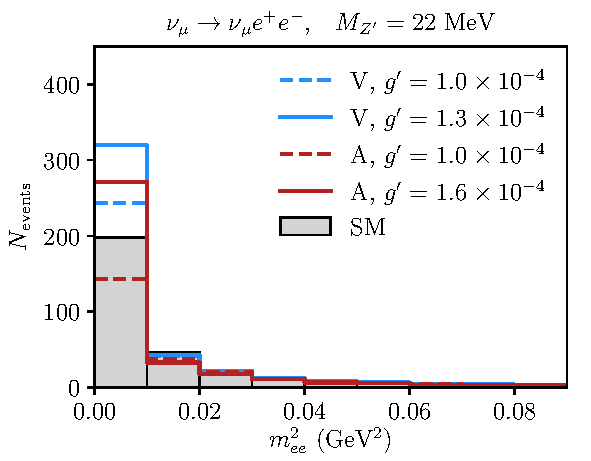
\includegraphics[width=0.4\textwidth]{BSM_invmass_ee.pdf}
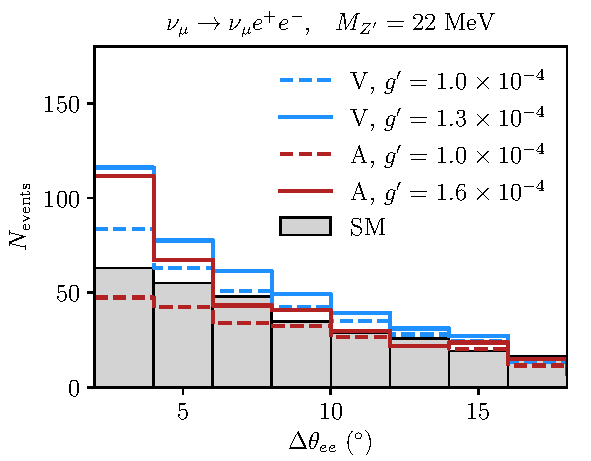
\includegraphics[width=0.4\textwidth]{BSM_sepangle_ee.pdf}
%
\caption{Same as \reffig{fig:mm_spectra} but for $e^+e^-$ trident events. In all cases we assume $Q^L_{\alpha}$ to be given by $L_e - L_\mu$. \label{fig:ee_spectra}}
%
\end{figure*}
%


\subsection{Neutrino-electron scattering}

Neutrino-electron scattering has long been a valuable probe of both the SM and potential new physics \cite{Marciano:2003eq,deGouvea:2006hfo,PhysRevD.93.093019,Lindner:2018kjo}. It is important to note that in the presence of novel leptophilic currents, experiments searching for $e^+e^-$ tridents would also observe anomalous $\nu-e$ event rates. In fact, given the larger statistics present in the $\nu-e$ scattering sample, this channel is expected to provide the leading constraints in our scenarios with tree-level couplings to electrons. 


In order to compute the $\nu-e$ cross section in the presence of the new leptophilic interactions we need to consider an analogous modification of the NC scattering amplitude
% neutrino-electron scattering amplitude in the presence of new physics. This is a purely leptonic amplitude and can be written as
\begin{align}
    \mathcal{M}_{\rm \nu_\alpha-e} = - \frac{G_F}{\sqrt{2}}  & \left[\bar{u}(k_2)\gamma^\mu(1-\gamma_5)u(k_1)\right] \nonumber\\ & \times \left[\bar{u}(p_2)\gamma_\mu(C^{\rm V}_\alpha-C^{\rm A}_\alpha\gamma_5)u(p_1)\right],
\end{align}
where the vector ($C_V$) and axial ($C_A$) effective couplings include both the SM and BSM contributions
%
\begin{subequations}
\begin{align}
%
C^{\rm V}_\alpha &= -\frac{1}{2}+2s^2_{\rm W} + \delta_{\alpha e} + \frac{Q^{\rm V}_{e} Q^{\rm L}_{\alpha} }{2\sqrt{2}G_F} \frac{(g^\prime)^2}{M_{Z^\prime}^2+2m_eT_e},\\
%
C^{\rm A}_\alpha &= -\frac{1}{2} + \delta_{\alpha e} + \frac{Q^{\rm A}_{e} Q^{\rm L}_{\alpha} }{2\sqrt{2} G_F} \frac{(g^\prime)^2}{ M_{Z^\prime}^2 + 2m_e T_e},
\label{eq:c_prescription_nue}
%
\end{align}
\end{subequations}
with, as usual, $s_{\rm W}\equiv\sin\theta_{\rm W}$, being $\theta_{\rm W}$ the weak angle and $T_e$ is the kinetic energy of the recoil electron. The loop-induced kinetic mixing in the $L_\mu-L_\tau$ model also induces a $\nu - e$ coupling
%
\begin{equation}
C^{\rm V}_\alpha = -\frac{1}{2}+2s^2_{\rm W} + \delta_{\alpha e} + \frac{1 }{\sqrt{2}G_F} \frac{g^\prime \, e\, \varepsilon(q^2)}{M_{Z^\prime}^2+2m_eT_e}.
\end{equation}
%
The differential cross section is then given by 
%
\begin{align}\label{nuexsection}
  \frac{d\sigma_{\nu_{\alpha}-e}}{dT_e} = \frac{2m_eG_F^2}{\pi} \Bigg[ \left(C^{\rm L}_\alpha\right)^2 &+\left(C^{\rm R}_\alpha\right)^2\left(1-\frac{T_e}{E_\nu}\right)^2\nonumber\\&-C^{\rm L}_\alpha C^{\rm R}_\alpha \, m_e \frac{T_e}{E_\nu^2} \Bigg].
\end{align}
%
where the left and right handed constants are given by
%
\begin{align*}
%
C^{\rm L}_\alpha \equiv \frac{1}{2}\left(C^{\rm V}_\alpha + C^{\rm A}_\alpha\right) \qquad\text{and}\qquad
%
C^{\rm R}_\alpha \equiv \frac{1}{2}\left(C^{\rm V}_\alpha - C^{\rm A}_\alpha\right).
%
\end{align*}
%
For antineutrino scattering one obtains the cross section by exchanging $C_{\alpha}^{\rm L} \leftrightarrow C_{\alpha}^{\rm R}$. 

The kinetic energy of the outgoing electron is bounded by kinematics and the energy resolution of the detector, which effectively sets a threshold energy $T_{\rm th}$ such that
%
\begin{align}
  T_{\rm th}  \le T_e \le T_{\rm max},
\end{align}
%   
with $T_{\rm max} = 2E_\nu^2/m_e+2E_\nu$, the maximum kinetic energy attainable. We define the effective total cross section for an initial neutrino energy $E_\nu$ as
%
\begin{equation}\label{eq:effective_nue_xsec}
\sigma_\text{eff}(E_\nu,T_\text{th}) = \int_{T_\text{th}}^{T_{\rm max}} \frac{d\sigma}{dT_e}\,dT_e.
\end{equation}
%
This definition also ensures that the enhancement due to very light mediators becomes constant at around $\sqrt{2 m_e T_\text{th}}$, as discussed in \refref{Lindner:2018kjo}. This is a consequence of the detector threshold and of the 2-body kinematics of the process. Finally, electroweak radiative corrections have been computed in the SM \cite{Bahcall:1995mm,Passera:2000ug}, but 
will not be included here. Since they correspond to a change of a few percent we do not expect them to affect very much our results.

\subsubsection{$\nu-e$ kinematical distributions \label{sec:nue_kinematics}}

\begin{figure*}[t]
%
\centering
%
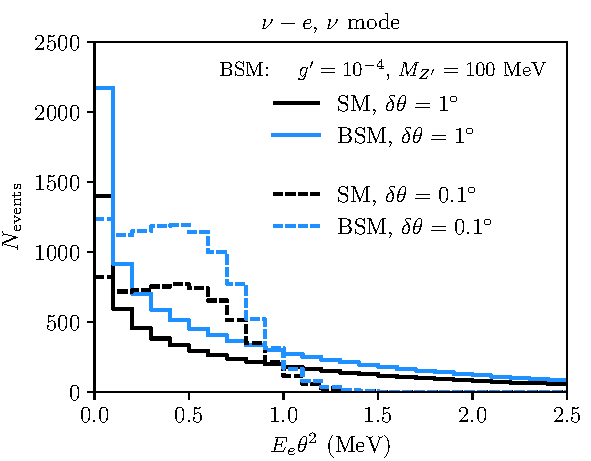
\includegraphics[width=0.43\textwidth]{Etheta2_nu_new.pdf}
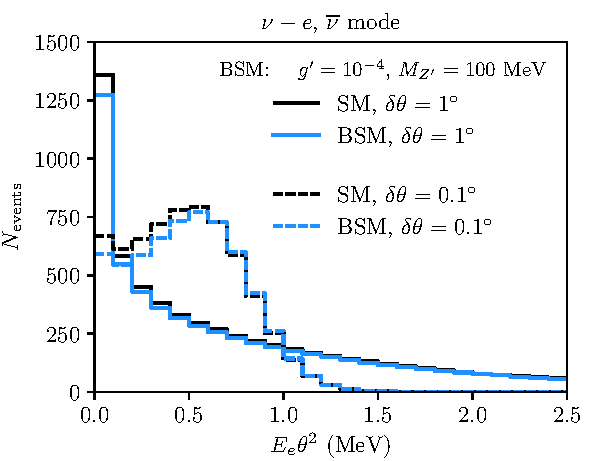
\includegraphics[width=0.43\textwidth]{Etheta2_nubar_new.pdf}
%
\caption{Number of $\nu-e$ scattering events in the DUNE ND as a function of $E_e\theta^2$ for the neutrino (left) and antineutrino (right) beams from the 120 GeV $p^+$ configuration. We show the prediction in the SM and in a vector $L_e-L_\mu$ $Z^\prime$ model for two angular resolutions $\delta\theta$. The electron kinetic energy threshold is taken to be $600$ MeV and the energy resolution is fixed at $\sigma/E = 15\%/\sqrt{E}$. \label{fig:nuedist}}
%
\end{figure*}


The angle between the scattered electron and the outgoing neutrino $\theta$ is related to their energies as 
%
\begin{align*} 
1 - \cos{\theta} = m_e \frac{1 - y}{E_e}, 
\end{align*}
%
where $y \equiv T_e/E_{\nu}$ is the inelasticity ($T_{\rm th}/E_{\nu}<y<1$) and $E_e=T_e+m_e$ is the outgoing electron energy. This implies that at ${\cal O}(\rm GeV)$ neutrino energies, the electron recoil is very forward and obey $E_e \theta^2 < 2 m_e$, up to detector resolution. For this reason, we choose to analyse our results in terms of  $E_e \theta^2$. In this case, the differential cross section becomes
\begin{eqnarray}
  \frac{d\sigma_{\nu_{\alpha}-e}}{d(E_e\theta^2)} =\frac{E_\nu}{2m_e}\frac{d\sigma_{\nu_{\alpha}-e}}{dT_e} \Bigg|_{T_e=E_\nu(1-\frac{E_e\theta^2}{2m_e})}\,.
\end{eqnarray}
This distribution is particularly important for suppressing the background. Given the kinematics explained above, $E_e\theta^2$ must be smaller than $2m_e$ for $\nu-e$ scattering, while it is often much larger for neutrino-nucleon scattering, the dominant background (See \refsec{sec:experimental}). We show in Fig.~\ref{fig:nuedist} the expected $\nu-e$ 
event distribution as a function of $E_e\theta^2$ for the SM and a light $Z^\prime$ case, in the neutrino and anti-neutrino modes at the DUNE ND. As expected, the signal is extremely forward and the final distribution is highly sensitive to the angular resolution $\delta\theta$ of the detector. At a conservative value of $\delta\theta = 1^\circ$, little information about the true distribution is left, and a significant portion of the signal lies in a region where $E_e\theta^2 > 2 m_e$. Therefore, shape information may improve the search for a light new physics only when the angular and energy resolutions of the detector are well understood. 
%%%%%%%%%

\subsection{Interference effects}

Since for $\nu-e$ scattering and neutrino trident production there exists a SM contribution, we expect the experimental sensitivity to new physics to be dominated by the interference between SM and BSM contributions. We now argue what kind of interference one can expect in each one of these processes.

For neutrino trident production we follow \refref{Brown1973} and separate the differential cross section as 
%
\begin{equation}
d\sigma = \hat{V}^2\,\, d\sigma_{\rm V} +\hat{V} \hat{A} \,d\sigma_{\rm V-A} + \hat{A}^2 \,d\sigma_{\rm A},
\end{equation}
%
where we dropped the flavour indices in $\hat{V}$ and $\hat{A}$ from (\ref{eq:c_prescription_trident}) for simplicity. This allows us to write the interference between the SM and the vector new physics as
%
\begin{equation}\label{eq:trident_interference}
d\sigma_{\rm{INT}} =  \frac{Q_{\alpha}^L Q_{\beta}^V}{2\sqrt{2} G_{F}} \frac{(g^\prime)^2}{K^2 + M^2_{Z^\prime}} \left( 2\, C_{\rm V}^{\rm SM}\, d\sigma_{\rm V}  + C_{\rm A}^{\rm SM} \, d\sigma_{\rm V-A}\right).
\end{equation}
%
Depending on the region of phase space considered, the term proportional to $d\sigma_{\rm V-A}$ can be of similar size to $d\sigma_{\rm V}$. However, $d\sigma_{\rm V-A}$ changes sign as a function of the angular variables or energies, leading to small integrated cross sections (typically two orders of magnitude smaller than the integral of the $d\sigma_{\rm V}$ term). Ignoring this term, one can then completely predict the type of interference in trident production. For $\nu_\mu \to \nu_\mu \mu^+ \mu^-$ trident production, for instance, $C_{\rm V}^{\rm SM} > 0$ and the second generation charge appears squared, leading to constructive interference in all cases. For $\nu_\mu \to \nu_\mu e^+e^-$ trident events, on the other hand, $C_{\rm V}^{\rm SM} < 0$. If the first and second generation charges come in with opposite signs, then the interference is still constructive, otherwise destructive interference happens. The same considerations also apply to antineutrino scattering if one ignores the $d\sigma_{\rm V-A}$ term. Finally, the axial-vector case is completely analogous taking $V \leftrightarrow A$ in \refeq{eq:trident_interference}.

For $\nu-e$ scattering analytical expressions can easily be used~\cite{Lindner:2018kjo}. Taking $C_L^{\rm{SM}}=-1/2+s_{\rm W}^2\sim-1/4$ and $C_L^{\rm{SM}}=s_{\rm W}^2\sim1/4$ we have
\begin{subequations}
    \begin{align}
        \frac{{d\sigma_{\rm{INT}}}_{\nu_\mu- e}}{dT_e}&\sim - \frac{\sqrt{2} m_e G_F}{4\pi}\frac{g'^2}{m_{Z'}^2+2m_eT_e}\left(-1+(1-y)^2\right)\\
        \frac{{d\sigma_{\rm{INT}}}_{\bar\nu_\mu- e}}{dT_e}&\sim - \frac{\sqrt{2} m_e G_F}{4\pi}\frac{g'^2}{m_{Z'}^2+2m_eT_e}\left(1-(1-y)^2\right).
    \end{align}
\end{subequations}
Since $y<1$, the interference term for $\nu_\mu- e$ is always positive (constructive), and for $\bar\nu_\mu -e$ it is always negative (destructive).

%%%%%%%%%%%%%%%%%%%%%%%%%%%%%%%%%%%%%%%%%%%%
\section{\label{sec:sensitivities}DUNE sensitivities}

Having studied the behaviour of neutrino trident production and neutrino-electron scattering cross sections in the presence of light new bosons, we now apply our results in sensitivity studies for the DUNE ND. As discussed in Section \ref{sec:models}, we limit our studies to $L_e- L_\mu$ and $L_\mu- L_\tau$ models with vector gauge bosons. We start with a discussion on the experimental details, highlighting the challenges of backgrounds and laying out our statistical methods in \refsec{sec:experimental}. Then we show our main results in Sections \ref{sec:le_lbeta} and \ref{sec:lmu_ltau}, comparing our sensitivity curves to the leading bounds in the parameter space of the leptophilic models from other experiments.

\subsection{Analysis techniques}\label{sec:experimental}

The LBNF is expected to produce an intense beam of neutrinos and antineutrinos from a 1.2 MW proton beam colliding against a fixed target \cite{Acciarri:2016crz}. The DUNE ND, where the number of neutrino interactions is the largest, is expected to be located at a distance of 574 m from the target. Despite its design not being final yet \cite{Roeck:2018,Manly:2018}, we focus on the possibility of a 75-t fiducial mass Liquid Argon (LAr) detector. Regarding the neutrino fluxes, we now concentrate on the option of a beam from 120 GeV protons with $1.1\times10^{21}$ POT per year. The LBNF could also provide higher or lower energy neutrinos depending on the proton energy, target and focusing system used. We explore other possibilities shown in \reftab{tab:rates} and we take the flux files provided in Ref.~\cite{DUNE:flux,DUNE:flux_updated}. We assume that the experiment will run 5 years in neutrino and another 5 years in antineutrino mode. The final exposure, therefore, will vary with beam designs, and is equal to a total of $11\times10^{22}$ POT in the case of 120 GeV protons. To generate neutrino scattering events, we use our own dedicated MC, Gaussian smearing the true MC energies and angles as a proxy for the detector effects during reconstruction. We assume an energy resolution of $\sigma/E = 15\%/\sqrt{E}$ $(\sigma/E = 6\%/\sqrt{E})$ for $e/\gamma$ showers (muons) and angular resolutions of $\delta\theta=1^\circ$ for all particles \cite{DUNECDRvolII}.

An interesting addition to the design of the DUNE ND would be a magnetized high-pressure Gaseous Argon (GAr) tracker placed directly behind the LAr module~\cite{DUNE:GArOption}. The lower thresholds for particle reconstruction and the presence of a magnetic field is expected to improve event reconstruction and reduce backgrounds to neutrino-electron scattering and neutrino trident production. We note that despite the relatively small fiducial mass of such a GAr module, $\lesssim 1$ tonne, it would still provide a sizeable number of these rare leptonic neutrino scattering processes. 

%%%%%%%%%%%%%%%%%%% TABLE %%%%%%%%%%%%%%%%%%%%%%%%%%%%%%%%%%%
\begin{table*}[t]
\begin{center}
\begin{tabular}{|lccccc|}
\hline
		Design & Mode & $\mu^+\mu^-$ trident & $e^+e^-$ trident & $\nu-e$ scattering & POTs/year \\ \hline\hline
		\multirow{ 2}{*}{62.4 GeV $p^+$}       &$\nu$ & $36.5$ & $92.7$ & $7670$ &  $1.83\times10^{21}$\\
		                     &$\overline{\nu}$ & $27.3$ & $73.4$ & $4620$ &  $1.83\times10^{21}$\\\hline
        \multirow{ 2}{*}{80 GeV $p^+$}         &$\nu$ & $42.0$ & $102$ & $8380$ &  $1.4\times10^{21}$\\ 
                             &$\overline{\nu}$ & $33.0$ & $84.3$ & $5320$ &  $1.4\times10^{21}$\\\hline 
        \multirow{ 2}{*}{120 GeV $p^+$}        &$\nu$ & $47.6$ & $110$ & $8930$ &  $1.1\times10^{21}$\\
                             &$\overline{\nu}$ & $40.7$ & $97.6$ & $6450$ &  $1.1\times10^{21}$\\\hline
        \multirow{ 2}{*}{$\nu_\tau$ app optm}  &$\nu$ & $210$ & $321$  & $24900$  & $1.1\times10^{21}$\\
                             &$\overline{\nu}$ & $156$ & $243$  & $14700$  &  $1.1\times10^{21}$\\
        \hline
\end{tabular}
\end{center}
\caption{The SM rates for neutrino trident production and neutrino-electron scattering per year at the 75-t DUNE ND after kinematical cuts. \label{tab:rates} }
\end{table*}

%%%%%%%%%%%%%%%%%%%%%%%%%%%%%%%%%%%%%%%%%%%%%%%%%%%%%%%%%%%%%%
With the intense flux at DUNE and the large number of POT, the $\nu-e$ scattering measurement will not be statistically limited, with order $10^4$ events in the DUNE ND after a few years. Systematics from the beam and detector are then the limiting factor for the sensitivity to new physics in this measurement. Current work on neutrino flux uncertainties shows that normalization uncertainties can be reduced to the order of $5\%$ \cite{Michael:2008bc,Aliaga:2013uqz,Abramov:2001nr}, with similar projections for DUNE \cite{Acciarri:2016crz}. The electron energy threshold also plays a role in the new physics search. In particular, for new light bosons the enhancement at very low momentum transfer $2 T_e m_e$ has a cut-off at the minimum electron recoil energy (see \refeq{eq:effective_nue_xsec}). This implies that the experiment is no longer sensitive to the $Z^\prime$ mass below $\sqrt{2 T_{\rm th} m_e}$. In our analysis, we assume a realistic overall normalization systematic uncertainty of $5\%$ and a $\nu-e$ scattering electron kinetic energy threshold of 600 MeV.

Lowering systematic uncertainties on the flux is challenging given the large hadroproduction and focusing uncertainties at the LBNF beam. Here, improvements on the experimental side in determining the neutrino flux will be extremely valuable (see \eg\ \refref{Bodek:2012uu}). If one is searching for novel leptophilic neutral currents, hadronic processes and inverse muon decay measurements are available, but these are limited either by theoretical uncertainties or by statistics, and might not be applicable in the whole energy region of interest. As to the electron energy, %our assumption 
assuming a threshold as low as $30$ MeV would be safe for electron detection, but at these low energies backgrounds can be incredibly challenging due to the overwhelming $\pi^0$ backgrounds. Increasing this threshold to $600$ MeV, however, has little impact in our sensitivities and is only $200$ MeV below the threshold used in the most recent MINER$\nu$A analysis \cite{Park:2013dax}, where good reconstruction is important for measuring the flux. For $e^+e^-$ and $\mu^+\mu^-$ tridents, we refrain from increasing the analysis thresholds from a naive $30$ MeV. This is certainly an aggressive assumption but it is necessary if $e^+e^-$ tridents are to be measured, since these events are quite soft \cite{Ballett:2018uuc}. Thresholds for $\mu^+\mu^-$ tridents are much less important since the events are generally more energetic than their dielectron analogue. 

\paragraph{Backgrounds ($\nu_\mu \to \nu_\mu \ell^+\ell^- $)}  We now discuss the individual sources of backgrounds to neutrino trident production. A pair of charged leptons is very rarely produced in neutrino interactions, usually coming from heavy resonance decays \cite{Conrad:1997ne,Astier:2000us,Adams:1999mn,Goncharov:2001qe,PhysRevD.43.2765}. Since our signal is mostly coming from coherent interactions with nuclei, cuts in the hadronic energy deposition in the detector $E_{\rm had}$, often large in heavy meson production processes, can help reduce backgrounds. Coherent and diffractive production of mesons is an exception to this, in particular pion production  \cite{Higuera:2014azj,Mislivec:2017qfz,Acciarri:2014eit,Acciarri:2015ncl}, which is the main background to trident due to particle mis-identification (misID). Muons are known to be easily spoofed by charged pions, making CC $\nu_\mu$ interactions with $\pi^\pm$ in the final state (CC1$\pi$) one of the largest contributions to the backgrounds of $\mu^+\mu^-$ tridents. Similarly, NC $\pi^0$ production stands as the leading background to $e^+e^-$ tridents when the photons are misIDed as two electrons, or if one of the photons pair converts and the other escapes detection. In Ref. \cite{Ballett:2018uuc}, we have shown that the $\mu^+\mu^-$ and $e^+e^-$ pairs produced in trident have small separation angles ($\Delta \theta$), possess small invariant masses ($m^2_{\ell \ell}$) and that both charged leptons are produced with small angles with respect to the neutrino beam ($\theta_{\pm}$). With simplified misID rates, we used the GENIE~\cite{Andreopoulos2009} event generator to show that simple kinematical cuts can reduce backgrounds significantly, achieving a significance of $S_{\mu\mu}/\sqrt{B_{\mu\mu}} \sim 44$ and $S_{ee}/\sqrt{B_{ee}} \sim 17.3$ for the DUNE ND in neutrino mode, where $S$ and $B$ stand for signal and background, respectively. In our current analysis we implement the same kinematical cuts, which are as follows: $m^2_{\mu \mu} < 0.2$ GeV$^2$, $\theta_{\pm} < 15^\circ$ and $\Delta \theta < 20^\circ$ for the $\mu^+\mu^-$ channel, and $m^2_{e e} < 0.1$ GeV$^2$, $\theta_{\pm} < 20^\circ$ and $\Delta \theta < 40^\circ$ for the $e^+e^-$ one. We impose these cuts again in our signal analysis, and point out that the new physics enhancement happens precisely in this favourable kinematical region, (see \refsec{sec:trident_kinematics}). Given the background rejection we find with our naive misID rates, we do not include backgrounds in our results, unless indicated otherwise.

\paragraph{Backgrounds ($\nu-e$)} For neutrino-electron scattering, backgrounds will arise from either the genuine production of an electron or via the misID of particle showers in the detector, both in the absence of observable hadronic energy deposition. The former scenario happens mostly by the CC interactions of the flux suppressed $\nu_e$ states present in the beam. The main contribution will be from CCQE interactions where the struck nucleon is invisible either for being below threshold or due to nuclear re-absorption. The misID of a photon initiated EM shower for an electron one is expected to be rare in LAr, where the first few cm of the showers can be used to separate electrons and photons by their characteristic $dE/dx$. However, the large NC rates for the production of single photons and $\pi^0$ can become a non-negligible background. For instance, coherent NC $\pi^0$ production leaves no observable hadronic signature and may look like a single electron if one of the photons is mis-identified and the other escapes detection. Finally, after misID happens, the signal can still look unique in its kinematical properties. In particular, $E_e \theta^2$ cuts can dramatically reduce backgrounds due to the forwardness of our signal (see e.g. \cite{Park:2013dax,Park:2015eqa}).

%
\begin{figure*}[t]
\centering
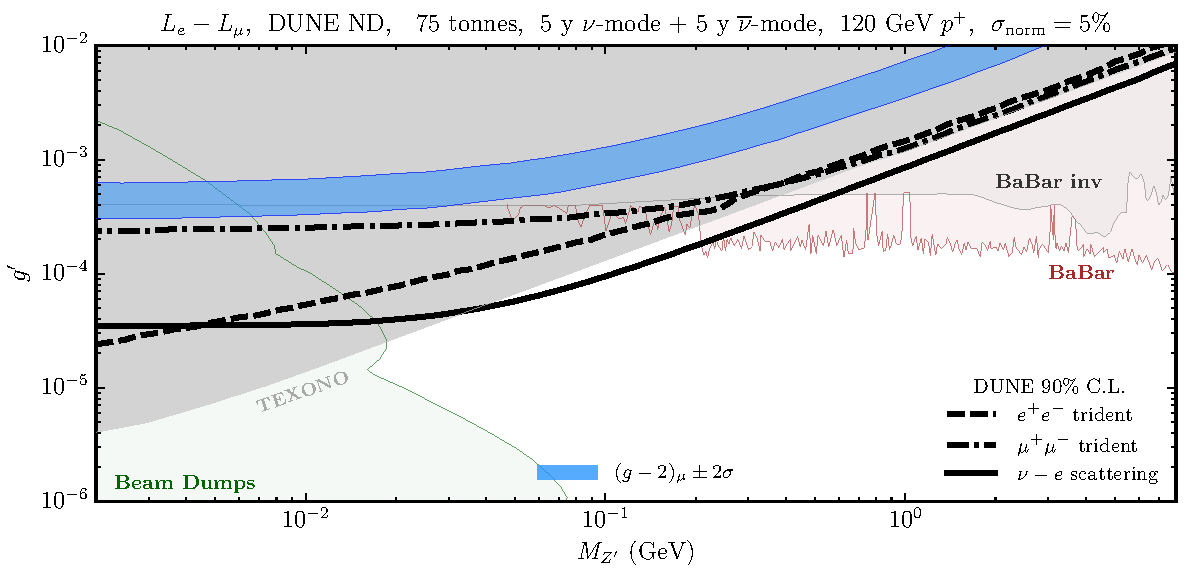
\includegraphics[width=0.8\textwidth]{lelmu.pdf}
 \caption{The DUNE ND neutrino scattering sensitivities to the $L_e - L_\mu$ $Z^\prime$ at 90\% C.L. The solid line shows the $\nu-e$ scattering sensitivity, followed by the dielectron trident in dashed line, and the dimuon trident in dot-dashed line. The coloured regions are excluded by other experiments, where we highlight the neutrino-electron scattering measurements at reactor experiments~\cite{Wong:2006nx,Deniz:2009mu,Chen:2014dsa}, searches at the BaBar $e^+e^-$ collider~\cite{Lees:2014xha, Lees:2017lec} and beam dump experiments~\cite{Bauer:2018onh}.\label{fig:Le_Lmu}}
\end{figure*}
%
\begin{figure*}[t]
\centering
    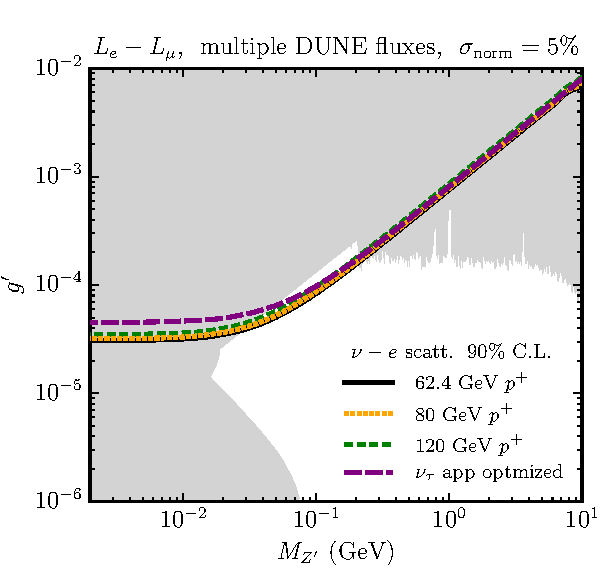
\includegraphics[width=0.43\textwidth]{lelmu_fluxes.pdf}
    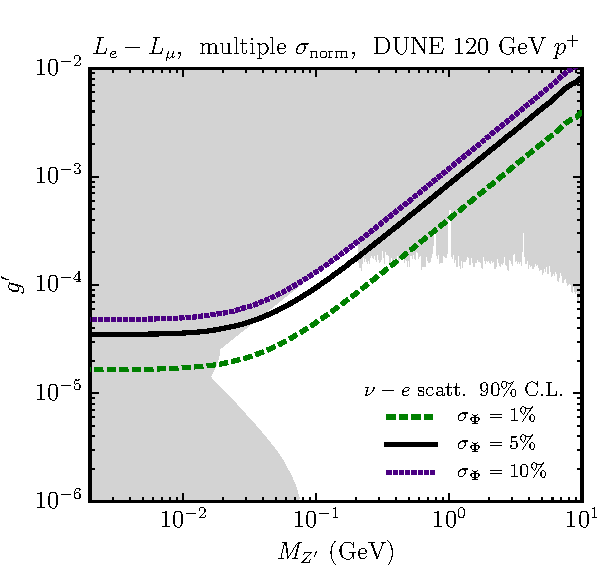
\includegraphics[width=0.43\textwidth]{lelmu_sys.pdf}
 \caption{The $\nu-e$ scattering sensitivity to the $L_e - L_\mu$ model at 90\% C.L. On the left panel we show the sensitivity using different choices for the neutrino flux, and on the right we use the neutrino beam from 120 GeV protons and vary the normalization systematic uncertainty from an aggressive $1\%$ to a conservative $10\%$. \label{fig:Le_Lmu_varied}}
\end{figure*}
%
\paragraph{Statistics.} 
In order to assess the potential of DUNE to discover new physics, we perform a sensitivity analysis using a $\chi^2$ test with a pull method for systematic uncertainties. Our goal is to assess when DUNE would be able to rule out the SM, and so we generate BSM events and fit the SM prediction to it. Our $\chi^2$ function is defined as
%
\begin{align}
  \chi^2 = \min_{\alpha} &\Bigg[\frac{ (N_{\text{BSM}} - (1+\alpha) N_{\text{SM}}-(\alpha+\beta) N_{\text{BKG}})^2 }{ N_{\text{BSM}}} \nonumber \\ &\quad \quad+ \left(\frac{\alpha}{\sigma_{\rm norm}}\right)^2 + \left(\frac{\beta}{\sigma_{\rm BKG}}\right)^2 \Bigg],
\end{align}
%
where the number of events for the BSM case is given by $N_{\rm BSM}$, the SM number of events is $N_{\rm SM}$ and the number of background events is $N_{\rm BKG}$. The nuisance parameters $\alpha$ and $\beta$, with their uncertainties $\sigma_{\rm norm}$ and  $\sigma_{\rm BKG}$, take into account normalization uncertainties from the flux and detector, and uncertainties on the background prediction, respectively. For the DUNE ND, we assume $\sigma_{\rm norm} = 5\%$ and $\sigma_{\rm BKG} = 10\%$. These systematics will likely be dominated by flux normalization uncertainties, and can only be measured with interactions that do not depend on the leptophilic BSM physics.

\subsection{\boldmath${L_e - L_\mu}$ \label{sec:le_lbeta}}

New vector bosons with couplings to the first and second generation leptons can be probed very effectively in neutrino experiments by meausuring the $\nu-e$ scattering rate. This has been recognized in the literature \cite{Bilmis:2015lja,Lindner:2018kjo,Bauer:2018onh}, where bounds from various experiments, including CHARM-II \cite{Vilain:1994qy}, TEXONO \cite{Wong:2006nx,Deniz:2009mu,Chen:2014dsa} and Borexino \cite{Bellini:2011rx} have been derived on these bosons. Curiously, the bound calculated from the CHARM-II data has been pointed out by \refref{Bauer:2018onh} to be too optimistic. The uncertainty on the neutrino flux is a real hindrance for these measurements which has not been taken into account when these bounds were computed. This is particularly important for measurements with large statistics, and for this reason we do not show the CHARM-II bound here. The measurement of $\overline{\nu}_e - e$ scattering at TEXONO, on the other hand, is statistically limited, and the bound it places on this class of models can safely ignore the flux systematics. This turns out to provide the strongest limit in a large region of the ${L_e - L_\mu}$ parameter space. Trident bounds can be obtained for this model, but due to their lower statistics and more involved kinematics, are subdominant.

We show our results for the DUNE ND in \reffig{fig:Le_Lmu}. Our results are for the combined $\nu+\bar\nu$ modes and do not include backgrounds. The opposite charges between the first and second families implies constructive interference between the SM and BSM contributions for neutrino scattering, contrary to what happens in a $B-L$ model, for instance. Therefore, the strongest bounds on this model can be obtained at DUNE in neutrino mode. It is clear, however, that the degree with which DUNE can probe unexplored parameter space is a question of how much the uncertainties on the flux can be lowered. To illustrate this effect, we vary the normalization systematics on the right panel of Fig.~\ref{fig:Le_Lmu_varied}, going from a conservative $10\%$ to an aggressive $1\%$ uncertainty. The effect of changing the thresholds is very small, being most important in a region already probed by other experiments. Different beam designs seem to have only a small impact 
on the sensitivity, as shown on the left panel of Fig.~\ref{fig:Le_Lmu_varied}.

Since we show the bounds obtained from the neutrino and antineutrino runs combined, it is not possible to see the effects of destructive interference. If only channels with destructive interference were available, however, it would have been possible to allow for cancellations between the total interference and the square of the BSM contributions in certain regions of parameter space at the level of the total rate. The region where this cancellation happens depends strongly on the neutrino energies involved and on the integrated phase space of the recoiled electron. In that case, one expects that the sensitivity to the lowest new physics couplings comes, in fact, from the search for a deficit of $\nu-e$ scattering events, as opposed to the constructive interference case where an excess of events is always produced. We note that this has no significant impact on the sensitivity of a leptophilic $Z^\prime$, but might provide crucial information about the nature of the $Z^\prime$ charges in case of detection. 

The trident bounds we obtain are not competitive for this model despite the fact that the trident cross sections receive similar enhancements to that of $\nu-e$ scattering. This is due to two reasons: the low number of events and the non-trivial kinematics of trident processes. Since the neutrino is essentially scattering off virtual charged leptons produced in the Coulomb field of the nucleus, it has to typically transfer more energy to the system than it would in a scattering off real particles in order to produce visible signatures. This remark also helps us to explain the behaviour of the sensitivity curves at the lowest masses. Whilst $\nu-e$ scattering cross sections become insensitive to the boson mass at $\sqrt{2 m_e T_{\rm th}}$, the trident cross sections do not. This behaviour is most dramatic in the $e^+e^-$ tridents, but is also present in the $\mu^+\mu^-$ one. This is a consequence of the 4-body phase space kinematics, where now the momentum transfer through the $Z^\prime$ propagator is no longer trivially related to the final state particle energies, as in $2\to2$ processes. It should be noted, however, that both the dimuon and the dielectron trident rates become nearly independent of $M_{Z^\prime}$ below the muon and the electron mass, respectively, where only a logarithmic dependence is expected~\cite{Altmannshofer2014}.

DUNE can also probe this class of models in a different way. In the context of long range forces in neutrino oscillation experiments and with the same choice of charges, Ref. \cite{Wise:2018rnb} places competitive bounds in this model with Super-Kamiokande data and makes projections for DUNE. The matter potential created by the local matter density modifies the dispersion relation of the neutrinos with lepton non-universal charges, leading to very competitive bounds in our region of interest. Similar considerations have also been explored in the context of high-energy astrophysical neutrinos~\cite{Bustamante:2018mzu}. Other experimental searches have been conducted at electron beam dumps. This technique consists of producing the $Z^\prime$ boson at the target via radiative processes such as $e + A \to e + A + Z^\prime$, and look for the visible decays of the boson in the detector. In this model, the decay products are mostly $e^+ e^-$ states and the bounds are only applicable at appreciably small values of $g^\prime$ and $M_{Z^\prime}$, where the lifetime of the $Z^\prime$ is sufficiently large. Probing the large mass region, on the other hand, requires high-energy experiments. In that regime, the strongest bounds come from searches at the $e^+ e^-$ collider BaBar. These come about in two ways: looking for the visible decay products of a $Z^\prime$ produced radiatively or in heavy meson decays \cite{Lees:2014xha}, or exploring the BR into invisible final states \cite{Lees:2017lec}.
%
\begin{figure*}[t]
\centering
  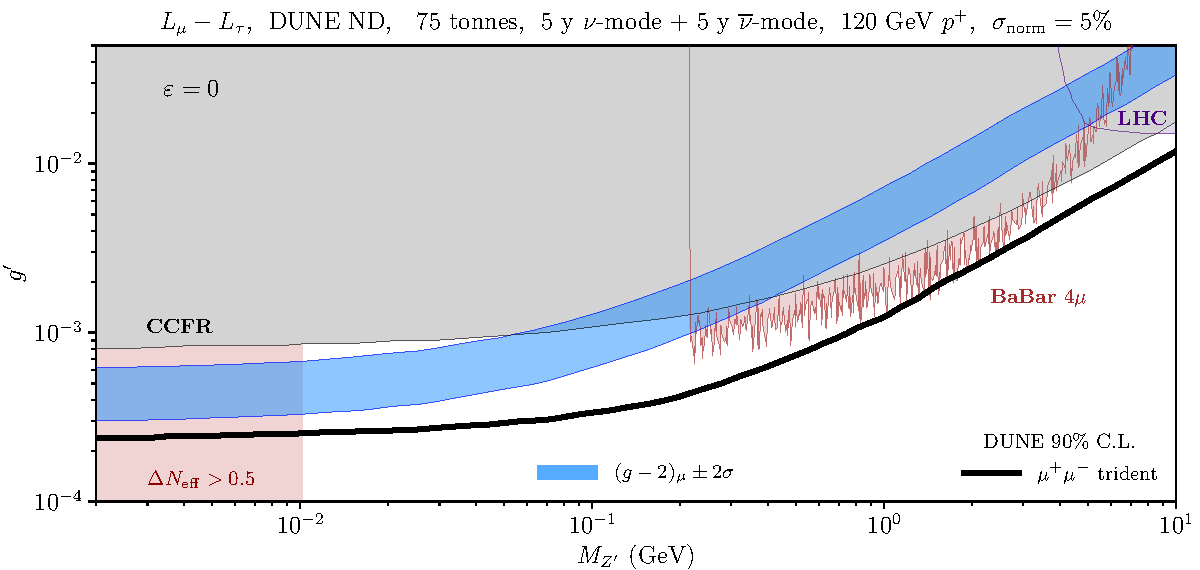
\includegraphics[width=0.8\textwidth]{lmultau_nokm.pdf}\\
 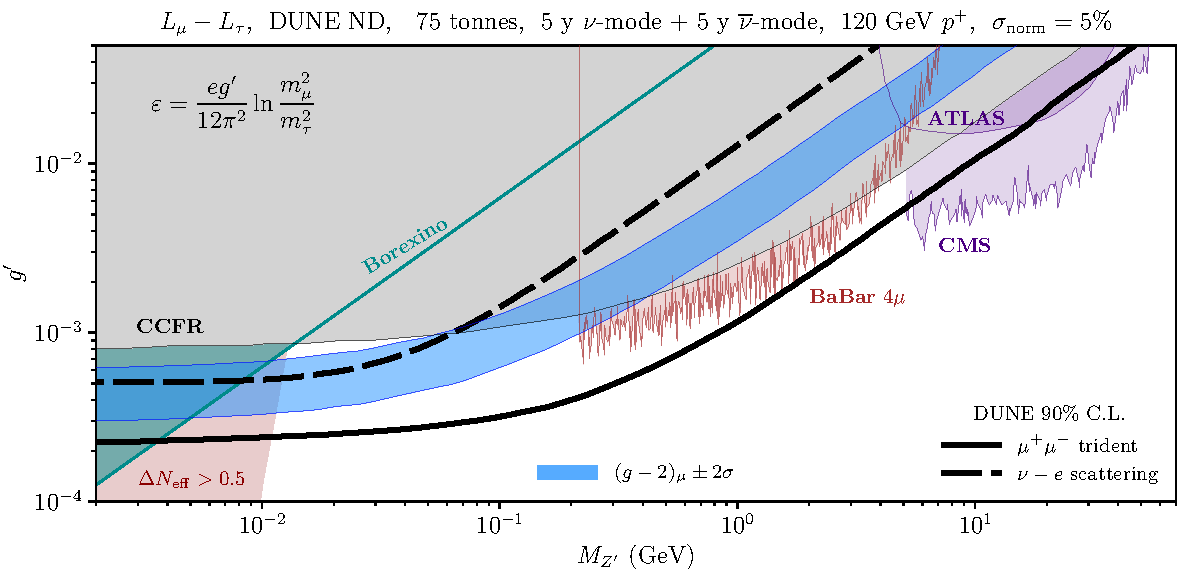
\includegraphics[width=0.8\textwidth]{lmultau_km.pdf}
 \caption{The DUNE ND neutrino scattering sensitivities for $L_\mu - L_\tau$ at 90\% C.L. The upper panel shows the case with no kinetic mixing, and the lower panel the case with the loop-induced mixing. Bounds from neutrino-electron scattering apply only to the latter. We also show bounds from BaBar~\cite{TheBABAR:2016rlg}, LHC~\cite{Aad:2014wra}, Borexino~\cite{Kaneta:2016uyt} and from the neutrino trident production measurement at CCFR~\cite{Mishra:1991bv,Altmannshofer2014}. Recent cosmological bounds for the two kinetic mixing cases derived in Ref.~\cite{Escudero:2019gzq} are also shown. \label{fig:Lmu_Ltau}}
\end{figure*}
%
%
\begin{figure*}[t]
\centering
  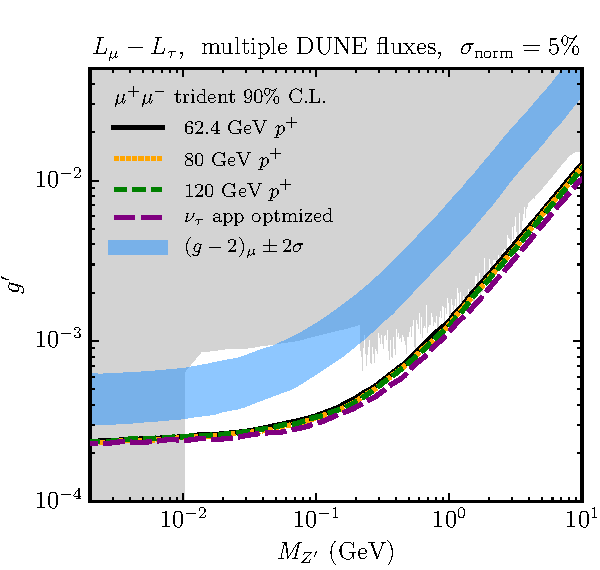
\includegraphics[width=0.43\textwidth]{lmultau_fluxes.pdf}
 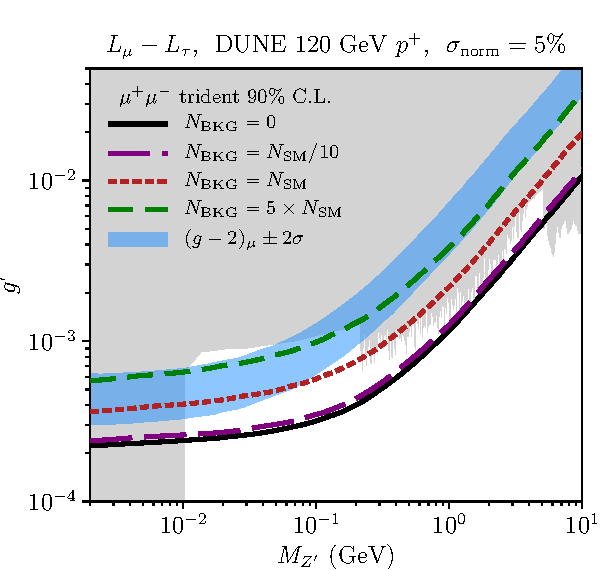
\includegraphics[width=0.43\textwidth]{lmultau_bkgs.pdf}
 \caption{The dimuon neutrino trident sensitivity to the $L_\mu - L_\tau$ model with no kinetic mixing at 90\% C.L. On the left panel we show the sensitivity using different choices for the neutrino flux, and on the right we use the neutrino beam from 120 GeV protons and scale the background with respect to the total number of SM trident events after cuts.\label{fig:Lmu_Ltau_varied}}
\end{figure*}
%

%%%%%%%%%%%%%%%%%%%%%%%%%%%%%%%%%%%%%%%%%%%%%%%%%%%%%%%%%%%%%%%%%%%%%%%%%%%%%%%%%%%
\subsection{\boldmath$L_\mu - L_\tau$ \label{sec:lmu_ltau}}

In this section we evaluate the DUNE ND sensitivity to the presence of a light
vector $Z^\prime$ charged under $L_{\mu} - L_{\tau}$. Beyond being anomaly free, this choice of charges allows for positive contributions to the anomalous magnetic moment of the muon, $a_\mu = (g-2)_{\mu}$, as discussed in Refs. \cite{Baek:2001kca,Pospelov:2008zw,Kamada:2015era,Araki:2015mya,Kamada:2018zxi}. This quantity is well known for a $\sim 3.7\sigma$ discrepancy between the experimental measurement \cite{Bennett:2006fi} and the theory predictions \cite{Blum:2018mom,Keshavarzi:2018mgv}. If future efforts to measure it \cite{Grange:2015fou} confirm this disagreement and if theoretical uncertainties are better controlled in the next few years, then constraining new physics scenarios that could contribute to $a_\mu$ is of utmost importance. 

This model can significantly impact neutrino trident production of a muon pair. In fact, the leading bound in this parameter space for masses $M_{Z^\prime} \lesssim 200$ MeV comes from the CCFR measurement of the same neutrino trident channel \cite{Mishra:1991bv}. CCFR observed $37.0\pm 12.4$ events, extracting a measurement of the trident cross section of $\sigma_{\rm CCFR}/\sigma_{\rm SM} = 0.82 \pm 0.28$. Curiously, the measurement by CHARM-II \cite{Geiregat:1990gz} provides weaker constraints on this model despite seeing a larger number of trident events, namely $55 \pm 16$ events in total, most likely due to the $1\sigma$ upward fluctuation of the measurement: $\sigma_{\rm CHARM-II}/\sigma_{\rm SM} = 1.58 \pm 0.57$. Other important bounds from $\nu-e$ scattering have also been obtained using the kinetic mixing parameter generated at one-loop. The strongest of which uses data from Borexino \cite{Kaneta:2016uyt}, and are only relevant for the low mass region $M_{Z^\prime} \lesssim 20$ MeV.

At DUNE, both of these measurements are possible, allowing to constrain this model in different ways. We show our results in Fig.~\ref{fig:Lmu_Ltau}, without including backgrounds. In this scenario, DUNE would be able to cover all the $2 \sigma$ region compatible with the $(g-2)_\mu$ measurement only with the $\mu^+ \mu^-$ trident events. For the low mass region, measuring the $\nu-e$ scattering rate can provide a complementary probe of this region, depending most strongly on the systematic uncertainties DUNE can achieve. We note that analysis thresholds used for $\nu-e$ scattering have little impact on the sensitivity in the region of interest. Our conclusion that DUNE can cover all of the $(g-2)_\mu$ region holds provided backgrounds are kept below the SM signal rate. This can be seen when we include backgrounds with different assumption on the right panel of Fig.~\ref{fig:Lmu_Ltau_varied}. Finally, different assumption for the beam design have little impact on the sensitivity, as show on the left panel of Fig.~\ref{fig:Lmu_Ltau_varied}.

Apart from neutrino scattering, dedicated searches for resonances decaying into $\mu^+ \mu^-$ in four muon final states have been performed at BaBar~\cite{TheBABAR:2016rlg}, looking for $e^+ e^- \to \mu^+\mu^- Z^\prime (\to \mu^+ \mu^-)$. At the LHC, the searches for $Z \to 4 \mu$~\cite{Aad:2014wra} performed by the ATLAS collaboration can be recast into a bound on $Z^\prime$. Here, we show the bounds derived in~\cite{Altmannshofer2014}. Big Bang Nucleosynthesis bounds were studied in~\cite{Kamada:2015era,Kamada:2018zxi}, and shown to constrain the mass of the boson to be $M_{Z^\prime} \gtrsim 5$ MeV. Recently, additional constraints from Cosmology were derived given that the presence of very light $Z^\prime$ bosons changes the evolution of the early Universe~\cite{Escudero:2019gzq}. In particular, the decays and inverse decays induced by the new leptophilic interactions can modify the neutrino relativistic degrees of freedom, requiring $M_{Z^\prime}\gtrsim 10$ MeV in order for $\Delta N_{\rm eff} < 0.5$ for the case with no kinetic mixing. The authors of Ref.~\cite{Escudero:2019gzq} also found that an additional $Z^\prime$ boson can alleviate the tension in the different measurements of the Hubble parameter. Let us stress here that all these bounds will be complementary to possible future constraints that can be obtained by the DUNE program, as shown in Fig.~\ref{fig:Lmu_Ltau}.

%%%%%%%%%%%%%%%%%%%%%%%%%%%%%%%%%%%%%%%%%%%%%%%%%%%%%%%%%%%%%%%%%%%%%%%%
\section{\label{sec:conclusion}Conclusions}
%%%%%%%%%%%%%%%%%%%%%%%%%%%%%%%%%%%%%%%%%%%%%%%%%%%%%%%%%%%%%%%%%%%%%%%%

Although the next generation neutrino oscillation experiments are primarily designed for making precision measurements of the neutrino mixing parameters, the unprecedented fluxes and large detectors will allow for many non-minimal new physics searches. In this work, we have considered the physics potential of the DUNE ND for constraining the existence of an additional anomaly-free $U(1)$ gauge group giving rise to a $Z^\prime$ boson which only couples to leptons --- a form of a purely leptophilic neutral current. Specifically, we have considered the anomaly free scenarios with charges associated to the lepton number difference $L_\alpha-L_\beta$.  Focusing on the two most promising neutrino scattering processes, $\nu- e$ and $\nu\ell\ell$ trident scattering, we have computed expected sensitivity curves for the DUNE ND for a variety of charge assignments. 

In performing our sensitivity studies as a function of the coupling and mass of the $Z^\prime$ boson, we have remained as faithful as possible to the real experimental conditions of a LAr detector. Our main results rely on the realistic assumptions of flux uncertainties of $5\%$ and feasible exposures. To avoid large backgrounds, we have also implemented kinematical cuts on the neutrino trident sample, and a kinetic energy threshold of $600$ MeV for $\nu-e$ scattering events. The parameter space which can be probed by $\nu-e$ scattering in the $L_e-L_\mu$ scenario is at least two times better than the $e^+e^-$ and almost twenty times better than the $\mu^+\mu^-$ trident channels, specially for the lower mass region. In this case, the DUNE ND would improve only slightly on previous $\nu-e$ scattering bounds, especially at around $M_{Z^\prime}\sim100$ MeV. We do not expect $e^+e^-$ trident  measurements at DUNE to improve our coverage of the $L_e - L_\mu$ $Z^\prime$ parameter space, but note this process has a distinct dependence on $M_{Z^\prime}$ if compared to $\nu-e$ scattering. 

If the light vector $Z^\prime$ is charged under $L_\mu-L_\tau$, we have found that the dimuon trident measurement could provide the leading bound in this parameter space. This is particularly interesting as these models can also explain the discrepancy between the measurement of the anomalous magnetic moment of the muon and its SM prediction. We expect that DUNE will be able to fully explore the $(g-2)_\mu$ motivated parameter space provided backgrounds are kept under control. The robustness of our results is tested against different choices of neutrino fluxes, where we find that despite the larger rates at higher neutrino energies and the larger BSM enhancement at lower energies, the sensitivities are very similar. 

Improvements to the experimental sensitivities we have displayed in Figs.~\ref{fig:Le_Lmu} and \ref{fig:Lmu_Ltau} can be achieved by reducing uncertainties on the neutrino flux and detection. From the experimental side, novel detection techniques suitable to rare neutrino events are currently under discussion, such as the magnetized HPgTPC~\cite{DUNE:GArOption} and the Straw Tube Tracker~\cite{PettiTalk,Duyang:2018lpe}. Together with improved analysis techniques, these will help to improve upon our projections for the sensitivity of DUNE to new physics that might be hiding at light masses and small couplings.



\chapter{A dark neutrino sector}
%%%%%%%%%%%%%%%%%%%%%%%%%%%%%%%%%%%%%%%%%%%%%%%%%%%%%
\graphicspath{{}{three_portals/}}

\begin{figure}[t]
\centering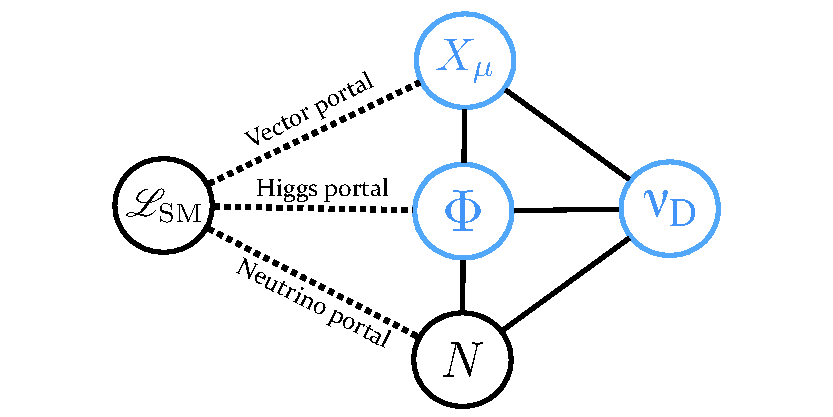
\includegraphics[width=0.7\textwidth]{three_portals/portals.pdf}
\caption{Schematic representation of our dark neutrino model. The dark neutrino, $\nu_{D}$ and the complex scalar $\Phi$ are the only fields charged under the new U$(1)^\prime$ gauge symmetry. The new vector boson $X_\mu$ acquires a mass after spontaneous symmetry breakig, and $N$ remains a complete singlet.
\label{fig:Tdiagrams}}
\end{figure}


\chapter{The MiniBooNE experimental anomaly}
%%%%%%%%%%%%%%%%%%%%%%%%%%%%%%%%%%%%%%%%%%%%%%%%%%%%%
\graphicspath{{}{three_portals/}}

\begin{figure}[t]
\centering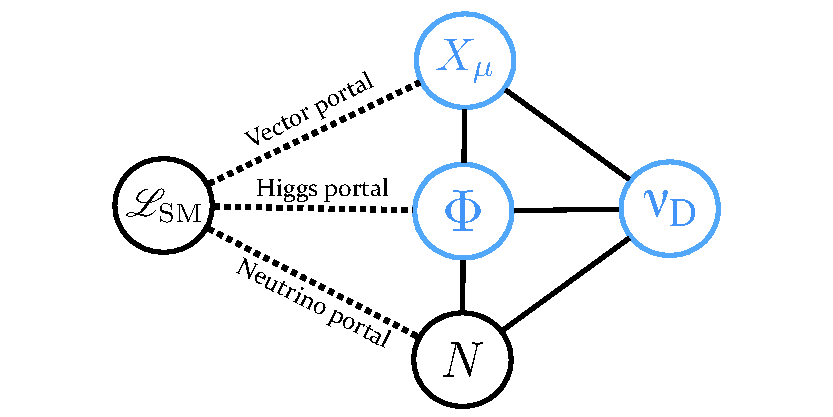
\includegraphics[width=0.7\textwidth]{three_portals/portals.pdf}
\caption{Schematic representation of our dark neutrino model. The dark neutrino, $\nu_{D}$ and the complex scalar $\Phi$ are the only fields charged under the new U$(1)^\prime$ gauge symmetry. The new vector boson $X_\mu$ acquires a mass after spontaneous symmetry breakig, and $N$ remains a complete singlet.
\label{fig:Tdiagrams}}
\end{figure}


\chapter{Future precision neutrino physics}
%%%%%%%%%%%%%%%%%%%%%%%%%%%%%%%%%%%%%%%%%%%%%%%%%%%%%
\graphicspath{{}{tridentSM/figs/}{tridentSM/}{Diagrams/}}

This chapter is dedicated to the study of rare neutrino scattering processes. Before we can explore the possibilities to constrain new physics, it is very important we understand our theoretical predictions in the SM. In this thesis we will see that leptonic and semi-leptonic neutrino scattering is a crucial tool to understanda and go beyond the SM. This chapter is dedicated to a refresher on neutrino-electron scattering and to original work developed on the calculation and phenomenology of neutrino trident scattering. These two processes were the object of study of experiments back in the 80's and 90's, but the high beam luminosity achieved at current neutrino experiments and expected at future facilitites (typically beyond $10^{21}$ protons on target), the relatively large fiducial masses of high-$Z$ materials (typically 100~ton) of modern detectors, and improved particle idenditification (PID) capabilities allows to return to this topic at lower energies ($E_\nu =$ few~GeV) with a refreshed approach.

\section{Neutrino-electron scattering}

Neutrino-electron scattering has long been a valuable probe of both the SM and potential new physics \cite{Marciano:2003eq,deGouvea:2006hfo,PhysRevD.93.093019,Lindner:2018kjo}. It is important to note that in the presence of novel leptophilic currents, experiments searching for $e^+e^-$ tridents would also observe anomalous $\nu-e$ event rates. In fact, given the larger statistics present in the $\nu-e$ scattering sample, this channel is expected to provide the leading constraints in our scenarios with tree-level couplings to electrons. 

In order to compute the $\nu-e$ cross section in the presence of the new leptophilic interactions we need to consider an analogous modification of the NC scattering amplitude
% neutrino-electron scattering amplitude in the presence of new physics. This is a purely leptonic amplitude and can be written as
\begin{align}
    \mathcal{M}_{\rm \nu_\alpha-e} = - \frac{G_F}{\sqrt{2}}  & \left[\bar{u}(k_2)\gamma^\mu(1-\gamma_5)u(k_1)\right] \nonumber\\ & \times \left[\bar{u}(p_2)\gamma_\mu(C^{\rm V}_\alpha-C^{\rm A}_\alpha\gamma_5)u(p_1)\right],
\end{align}
where the vector ($C_V$) and axial ($C_A$) effective couplings include both the SM and BSM contributions
%
\begin{subequations}
\begin{align}
%
C^{\rm V}_\alpha &= -\frac{1}{2}+2s^2_{\rm W} + \delta_{\alpha e} + \frac{Q^{\rm V}_{e} Q^{\rm L}_{\alpha} }{2\sqrt{2}G_F} \frac{(g^\prime)^2}{M_{Z^\prime}^2+2m_eT_e},\\
%
C^{\rm A}_\alpha &= -\frac{1}{2} + \delta_{\alpha e} + \frac{Q^{\rm A}_{e} Q^{\rm L}_{\alpha} }{2\sqrt{2} G_F} \frac{(g^\prime)^2}{ M_{Z^\prime}^2 + 2m_e T_e},
\label{eq:c_prescription_nue}
%
\end{align}
\end{subequations}
with, as usual, $s_{\rm W}\equiv\sin\theta_{\rm W}$, being $\theta_{\rm W}$ the weak angle and $T_e$ is the kinetic energy of the recoil electron. The loop-induced kinetic mixing in the $L_\mu-L_\tau$ model also induces a $\nu - e$ coupling
%
\begin{equation}
C^{\rm V}_\alpha = -\frac{1}{2}+2s^2_{\rm W} + \delta_{\alpha e} + \frac{1 }{\sqrt{2}G_F} \frac{g^\prime \, e\, \varepsilon(q^2)}{M_{Z^\prime}^2+2m_eT_e}.
\end{equation}
%
The differential cross section is then given by 
%
\begin{align}\label{nuexsection}
  \frac{d\sigma_{\nu_{\alpha}-e}}{dT_e} = \frac{2m_eG_F^2}{\pi} \Bigg[ \left(C^{\rm L}_\alpha\right)^2 &+\left(C^{\rm R}_\alpha\right)^2\left(1-\frac{T_e}{E_\nu}\right)^2\nonumber\\&-C^{\rm L}_\alpha C^{\rm R}_\alpha \, m_e \frac{T_e}{E_\nu^2} \Bigg].
\end{align}
%
where the left and right handed constants are given by
%
\begin{align*}
%
C^{\rm L}_\alpha \equiv \frac{1}{2}\left(C^{\rm V}_\alpha + C^{\rm A}_\alpha\right) \qquad\text{and}\qquad
%
C^{\rm R}_\alpha \equiv \frac{1}{2}\left(C^{\rm V}_\alpha - C^{\rm A}_\alpha\right).
%
\end{align*}
%
For antineutrino scattering one obtains the cross section by exchanging $C_{\alpha}^{\rm L} \leftrightarrow C_{\alpha}^{\rm R}$. 

\subsection{Kinematics} The kinetic energy of the outgoing electron is bounded by kinematics and the energy resolution of the detector, which effectively sets a threshold energy $T_{\rm th}$ such that
%
\begin{align}
  T_{\rm th}  \le T_e \le T_{\rm max},
\end{align}
%   
with $T_{\rm max} = 2E_\nu^2/m_e+2E_\nu$, the maximum kinetic energy attainable. We define the effective total cross section for an initial neutrino energy $E_\nu$ as
%
\begin{equation}\label{eq:effective_nue_xsec}
\sigma_\text{eff}(E_\nu,T_\text{th}) = \int_{T_\text{th}}^{T_{\rm max}} \frac{d\sigma}{dT_e}\,dT_e.
\end{equation}
%
This definition also ensures that the enhancement due to very light mediators becomes constant at around $\sqrt{2 m_e T_\text{th}}$, as discussed in \refref{Lindner:2018kjo}. This is a consequence of the detector threshold and of the 2-body kinematics of the process. Finally, electroweak radiative corrections have been computed in the SM \cite{Bahcall:1995mm,Passera:2000ug}, but 
will not be included here. Since they correspond to a change of a few percent we do not expect them to affect very much our results.


\subsection{Measurements}

MINERvA

CHARM-II, CHARM, 

TEXONO, GEMMA, DAYA BAY?

Solar neutrinos - BOREXINO, SNO, Super-K

\section{Neutrino trident scattering}

Trident events are processes predicted by the SM as the result of (anti)neutrino-nucleus scattering with the production of a charged lepton pair \cite{Czyz:1964zz,Lovseth:1971vv,Fujikawa:1971nx,Brown:1971qr,Koike:1971tu}, $\pbar{\nu}_{\alpha}+{\cal{H}} \to \pbar{\nu}_{\alpha \,{\rm{or}} \, \kappa(\beta)} + \ell_{\beta}^- + \ell_\kappa^+ +{\cal{H}}$, $\{\alpha,\beta,\kappa\}\in \{e,\mu,\tau\}$\footnote{Throughout the manuscript we will consider ${\alpha,\beta, \kappa}$ as flavour indexes.} where $\cal{H}$ denotes a hadronic target. Depending on the (anti)neutrino and charged lepton flavours in the final-state, the process will be mediated by the $Z^0$ boson, $W$ boson or both. Coherent interactions between (anti)neutrinos and the atomic nuclei are expected to dominate these processes as long as the momentum transferred $Q$ is significantly smaller than the inverse of the nuclear size \cite{Czyz:1964zz}. For larger momentum transfers incoherent elastic and deep-inelastic scattering become increasingly relevant \cite{Magill:2016hgc}.
%
Although this process exists for all combinations of same-flavour or mixed flavour charged-lepton final-states, to this day only the $\nu_\mu$-induced dimuon mode, $\pbar{\nu}_\mu + {\cal{H}} \to \pbar{\nu}_\mu  + \mu^+ + \mu^- + {\cal{H}}$, has been observed. The first measurement of this trident signal performed by CHARM II~\cite{Geiregat:1990gz} is also the one with the largest statistics: 55 signal events in a beam of neutrinos and antineutrinos with $\langle E_\nu \rangle \approx 20$ GeV. Other measurements by CCFR~\cite{Mishra:1991bv} and NuTeV~\cite{Adams:1998yf} at larger energies soon followed.

As the measurement of trident events may provide a sensitive test of the weak sector~\cite{Brown:1973ih} as well as placing constraints on physics beyond the SM~\cite{Mishra:1991bv,Gaidaenko:2000hg,Altmannshofer:2014pba,Kaneta:2016uyt,Ge2017,Magill:2017mps,Falkowski:2018dmy} it is relevant to investigate how to probe it further at current and future neutrino experiments. Atmospheric neutrinos, for instance, may provide a feasible measurement of the dimuon channel, as pointed out in \refref{Ge2017}\footnote{The authors of \refref{Ge2017} have performed the full calculation of the trident process and made their code publicly available.}. Other trident modes were also re\-cog\-ni\-zed to be relevant by the authors of Ref.~\cite{Magill:2016hgc} who calculated the cross sections for trident production in all possible flavour combinations and estimated the number of events expected for the DUNE and SHiP experiments. They used the Equivalent Photon Approximation (EPA)~\cite{Belusevic:1987cw} to compute the cross section in the coherent and incoherent regimes of the scattering. The EPA, however, is known to breakdown for final state electrons~\cite{Kozhushner:1962aa, Shabalin:1963aa, Czyz:1964zz} leading, as we will demonstrate here, to an overestimation of the cross section that in some cases is by more than 200\%. 

In this work, we present a unified treatment of the coherent and incoherent trident calculation beyond the EPA for all modes. We then compute the number and distribution of events expected in each mode at various near detectors, devoting particular attention to the case of liquid argon (LAr) detectors, as they are expected to lead the field of precision neutrino scattering measurements over the next few decades thanks to their excellent tracking and calorimetry capabilities. Finally, we address the likely backgrounds that may hinder these experimental searches --- a question that we believe to be of utmost importance given the rarity of the process, and one that has been omitted in earlier sensitivity studies \cite{Magill:2016hgc,Altmannshofer:2014pba}. 

This paper is organized as follows. In Sec.~\ref{sec:xsec}, we explain how to correctly calculate the trident SM cross sections, comparing our results to the EPA and explicitly showing the breakdown of this approximation. In Sec.~\ref{sec:LAr}, we discuss the trident event rates and kinematic distributions at the near detectors of several present and future neutrino oscillation experiments based on LAr technology: the three detectors of the Short-Baseline Neutrino (SBN) Program at Fermilab~\cite{SBNproposal} and the near detector for the long-baseline Deep Underground Neutrino Experiment (DUNE)~\cite{Acciarri:2016ooe,DUNECDRvolII}, also located at Fermilab. We also consider the potential gains from an optimistic future facility: a 100 t LAr detector subject to the novel low-systematics neutrino beam of the Neutrinos from STORed Muons ($\nu$STORM) project~\cite{Soler:2015ada,nuSTORM2017}. 
%
We discuss the sources of background events at these facilities, providing a GENIE-level analysis \cite{Andreopoulos2009} of how to reduce these backgrounds and assessing the impact they are expected to have on the trident measurement. 
%
In Sec.~\ref{sec:others}, we discuss other near detectors that use more conventional technologies: the Interactive Neutrino GRID (INGRID)~\cite{Abe:2011xv,Abe:2015biq,Abe:2016fic,Abe:2016tez}, the on-axis iron near detector for T2K at J-PARC, as well as three detectors at the Neutrino at the Main Injector (NuMI) beamline at Fermilab, the one for the Main INjector ExpeRiment $\nu$-A (MINER$\nu$A)~\cite{Altinok:2017xua,MINERvA:2017} and the near detectors for the Main Injector Oscillation Search (MINOS)~\cite{Adamson:2014pgc,AlpernBoehm} and the Numi Off-axis $\nu_e$ Appearance (NO$\nu$A) experiment~\cite{Wang:Biao,sanchez_mayly_2018_1286758}. 
%

%%%%%%%%%%%%%%%%%%%%%%%%%%%%%%%%%%%%%%%%%%%%%%%%%%%%
\section{Trident Production Cross Section}\label{sec:xsec}

In this section we consider neutrino trident production in the SM, defined as the process where a (anti)neutrino scattering off a hadronic system ${\cal H}$ produces a pair of same-flavour or mixed flavour charged leptons 
%
\begin{equation}
\pbar{\nu}_{\alpha}(k_1) \,+\, {\cal H}(P) \,\to\, \pbar{\nu}_{\alpha^\prime} (k_2) \,+\, \ell_\beta^- (p_-)  \,+\, \ell_\kappa^+ (p_+) \,+\, {\cal H}(P^\prime),
\label{eq:indices}
\end{equation}
%
where $\beta (\kappa)$ corresponds to the flavour index of the negative (positive) charged lepton in both neutrino and antineutrino cases. 
%
Neutrino trident scattering can be divided into three regimes depending on the nature of the hadronic target: coherent, incoherent elastic and deep inelastic, when the neutrino scatters off the nuclei, nucleons and quarks, respectively. At the energies relevant for neutrino oscillation experiments, the deep inelastic scattering contribution amounts at most to 1\% of the total trident production cross section \cite{Magill:2016hgc} and we will not consider it further.

The cross section for trident production has been calculated before in the literature, both in the context of the $V-A$ theory~\cite{Czyz:1964zz,Lovseth:1971vv,Fujikawa:1971nx} and in the SM~\cite{Brown:1973ih}, while the EPA treatment was developed in Refs.~\cite{Kozhushner:1962aa,Shabalin:1963aa,Belusevic:1987cw}. Most calculations have focused on the coherent channels \cite{Czyz:1964zz,Lovseth:1971vv,Fujikawa:1971nx,Brown:1973ih,Belusevic:1987cw} but the incoherent process has been considered in \cite{Czyz:1964zz,Lovseth:1971vv}. More recently, calculations using the EPA have been performed for coherent scattering with a dimuon final-state \cite{Altmannshofer:2014pba}, and for all combinations of hadronic targets and flavours of final-states in \cite{Magill:2016hgc}. While the EPA is expected to agree reasonably well with the full calculation for coherent channels with dimuon final-states, the assumptions of this approximation are invalid for the coherent process with electrons in the final-state \cite{Kozhushner:1962aa,Shabalin:1963aa,Czyz:1964zz}. 
%
For this reason, we perform the full $2\to 4$ calculation without the EPA in a manner applicable to any hadronic target, following a similar approach to Refs.~\cite{Czyz:1964zz,Lovseth:1971vv}. Our treatment of the cross section allows us to quantitatively assess the breakdown of the EPA in both coherent and incoherent channels for all final-state flavours, an issue we come back to in Sec.~\ref{sec:EPAbreakdown}.

We write the total cross section for neutrino trident production off a nucleus ${\cal N}$ with $Z$ protons and $(A-Z)$ neutrons as the sum
%
\begin{equation}
\sigma_\mathrm{\nu {\cal N}} = \sigma_\mathrm{\nu c} +\sigma_\mathrm{\nu d}\, ,
\end{equation}
where $\sigma_\mathrm{\nu c}$ ($\sigma_\mathrm{\nu d}$) is the coherent (incoherent) part of the cross section. 
%
%%%%%%%%%%%% SM DIAGRAMS %%%%%%%%%%%%%%%%
\unitlength = 0.9mm
\begin{figure}[t]
% \centering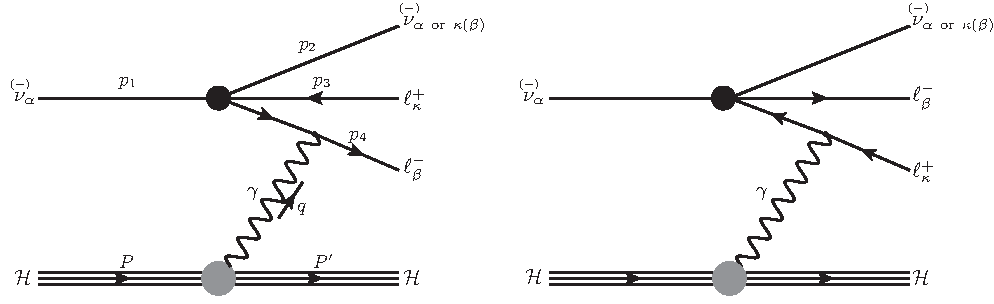
\includegraphics[width=\textwidth]{tridentSM/figs/SM-trident.pdf}
\centering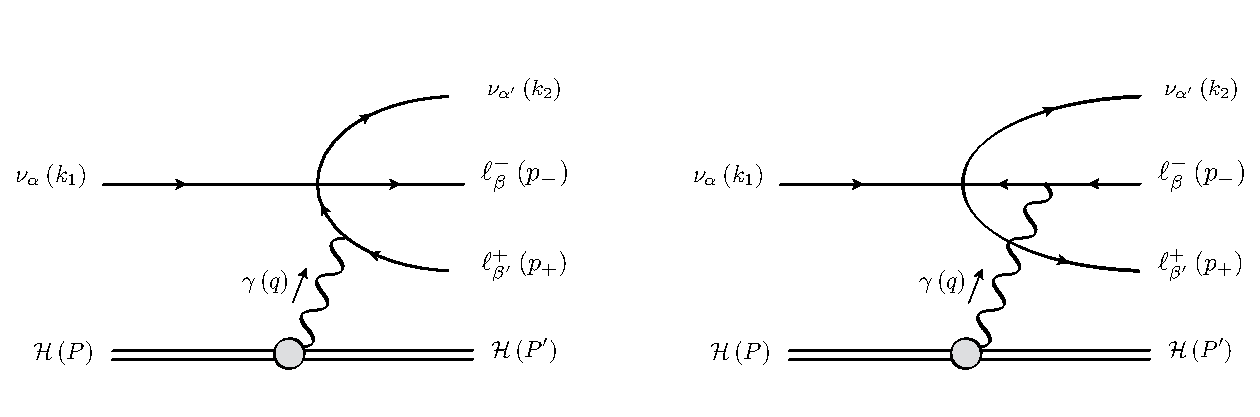
\includegraphics[width=\textwidth]{Neutrino_trident_production.pdf}
\caption[Neutrino trident production with a contact approximation.]{Diagrams contributing to the neutrino trident process in the four-point interaction limit of the Standard Model.  
\label{fig:Tdiagrams}}
\end{figure}

%%%%%%%%%%%%%%%%%%%%%%%%%%%%%%%%%%%%%%%%%
%
The relevant diagrams for these processes in the coherent or incoherent 
regimes involve the boson $Z^0$, $W$ or both mediators, depending on the particular mode. In the four-point interaction limit, depicted in \reffig{fig:Tdiagrams}, these reduce to only two contributions\footnote{An additional diagram involving a $WW\gamma$ vertex has also been neglected, since it is of order $1/M_W^4$.}, one where the photon couples to the negatively and one to the positively charged lepton. 
In Table \ref{tab:tridentmodes}, we present the processes we will consider in this thesis as well as the SM contributions present in each. Although our formalism applies also to processes with final-state $\tau$ leptons, the increased threshold and their suppressed cross section makes them irrelevant for the experiments of interest in this study and we do not consider them further.
%
The trident amplitude for a coherent (${\rm X=c}$) or incoherent (${\rm X=d}$) scattering regime can be written as
%
\begin{equation}
i \mathcal{M} = \mathrm{L}^\mu (\{p_i\},q) \, \frac{-ig_{\mu \nu}}{q^2} \, \mathrm{H}_{\rm X}^{\nu}(P,P^{\prime})\, ,
\end{equation}
%
where $\{p_i\}=\{k_2,p_-,p_+\}$ is the set of outgoing leptonic momenta. $ \mathrm{L}^\mu (\{p_i\},q)$ is the total leptonic amplitude 
%
\begin{align}
\mathrm{L}^\mu & \equiv - \frac{ie G_F}{\sqrt{2}}[\bar{u}(k_2)\gamma^\tau(1-\gamma_5)u(k_1)] \times 
\bar{u}(p_-)\left[\gamma_\tau(V-A\gamma_5)\frac{1}{(\slashed{q}-\slashed{p}_+ - m_+)}\gamma^\mu \right . \nonumber \\ 
& \left . + \gamma^\mu \frac{1}{(\slashed{p}_- -\slashed{q}-m_-)} \gamma_\tau (V-A \gamma_5) \right] v(p_+)\, ,
\label{eq:Lmu}
\end{align}
%
and $\mathrm{H}_{\rm X}^{\nu}(P,P^{\prime})$ is the total hadronic amplitude
\begin{align}
H_{\rm X}^\nu  &\equiv \langle {\cal H}(P) \vert J_\mathrm{E.M.}^\nu (q^2)\vert {\cal H}(P^\prime)\rangle\, ,
\label{eq:Hmu}
\end{align}
%
with  $q \equiv P - P^\prime$ denoting the transferred momentum, $m_+$ ($m_-$) the positively (negatively) charged lepton mass and ${J}^\nu_{\rm{E.M.}} (q^2)$ the electromagnetic current for the hadronic system ${\cal H}$ (a nucleus or a nucleon). The flavour indices have been ommitted from the vector $V$ and axial $A$ couplings, determined by $V \equiv g_{V}^{\alpha^\prime} \delta_{\alpha\alpha^\prime}\delta_{\beta\beta^\prime}+\delta_{\alpha^\prime \beta^\prime}\delta_{\alpha\beta}$ and $A \equiv g_{A}^{\alpha^\prime} \delta_{\alpha\alpha^\prime}\delta_{\beta\beta^\prime}+\delta_{\alpha^\prime \beta^\prime}\delta_{\alpha\beta}$ in accordance to~\refeq{eq:indices} and shown in~\reftab{tab:tridentmodes}.
%
\begin{table}[t]
\begin{center}
\begin{tabular}{cccc}
\hline
Trident channel &  SM Contributions & V & A \\
\hline
${\nu}_\mu\, {\cal H} \to {\nu}_\mu\, \mu^- \mu^+\,  {\cal H}$  & CC + NC &$\sfrac{1}{2} + 2 \,\sw^2$&$\sfrac{1}{2}$\\
${\nu}_\mu\, {\cal H} \to {\nu}_\mu\,  e^- e^+\, {\cal H}$ & NC&$-\sfrac{1}{2} + 2 \,\sw^2$&$-\sfrac{1}{2}$\\
${\nu}_\mu\, {\cal H} \to {\nu}_e\,  e^+ \mu^-\, {\cal H}$  & CC&$1$&$1$\vspace{2ex}\\
${\nu}_e\, {\cal H} \to {\nu}_e\,  e^- e^+\, {\cal H}$ &  CC + NC &$\sfrac{1}{2} + 2 \,\sw^2$&$\sfrac{1}{2}$\\
${\nu}_e\, {\cal H} \to {\nu}_e\,  \mu^- \mu^+\, {\cal H}$ & NC &$-\sfrac{1}{2} + 2 \,\sw^2$&$-\sfrac{1}{2}$\\
${\nu}_e\, {\cal H} \to {\nu}_\mu\,  \mu^+ e^-\, {\cal H}$ & CC &$1$&$1$\\

\hline
\end{tabular}
\end{center}
\caption[Neutrino trident production channels and their SM contributions.]{\label{tab:tridentmodes} Neutrino trident processes considered in this thesis. Antineutrino induced channels are analogous.}
\end{table}
%

We can write the differential cross section as
\begin{align}
\frac{\dd^2 \sigma_{\nu  {\rm X}}}{\dd Q^2 \dd \hat{s}}= \frac{1}{32  \pi^2(s-M_{\cal H}^2)^2}\frac{\mathrm{H}_{\rm X}^{\mu\nu}\mathrm{L}_{\mu\nu}}{Q^4}\, ,
\end{align}
where $s = (k_1 + P)^2$, $\hat{s} \equiv 2\,(k_1 \vdot q)$, $Q^2 = -q^2$ and $M_{\cal H}$ is the mass of the hadronic target. We have also introduced the hadronic tensor $\mathrm{H}_{\rm X}^{\mu \nu}$
%
\begin{align}
\mathrm{H}_{\rm X}^{\mu\nu} &\equiv \overline{\sum_{\rm{spins}}}  \left(\mathrm{H}_{\rm X}^\mu\right)^* \mathrm{H}_{\rm X}^\nu.
%
\end{align}
The two scattering regimes in which the hadronic tensor is computed will be discussed in more detail in Sec.~\ref{sec:had}. The leptonic tensor, $\mathrm{L}^{\mu \nu}$, integrated over the phase space of the three final-state leptons, $\dd^{3} \Pi \left(k_1 + q; \{p_i\}\right)$, and merely summed over final and initial spins is given by
%
\begin{equation}
\mathrm{L}^{\mu \nu} (k_1, q) \equiv  \int \dd ^{3} \Pi \left(k_1 + q; \{p_i\}\right) \left( \sum_{\rm{spins}} \left(  \mathrm{L}^\mu \right)^*  \mathrm{L}^\nu  \right)\, .
\label{eq:Lmunu}
\end{equation}
We can use $\mathrm{L}^{\mu \nu}$ to define two scalar functions, one related to the longitudinal ($\mathrm{L}_{\mathrm{L}}$) and the other to the transverse ($\mathrm{L}_{\mathrm{T}}$) polarization of the exchanged photon
\begin{equation}
\mathrm{L}_{\mathrm{T}} = -\frac{1}{2}\left( g^{\mu \nu} - \frac{4Q^2}{\hat{s}^2} k_1^\mu k_1^\nu \right) \mathrm{L}_{\mu \nu}, \quad \mathrm{and} \quad \mathrm{L_{L}} =  \frac{4Q^2}{\hat{s}^2} k_1^\mu k_1^\nu \mathrm{L}_{\mu \nu}\, .\label{eq:LT_LL}
\end{equation}
%
This allows us to write the differential cross section as a sum of a longitudinal and a transverse contribution \cite{Hand:1963bb} as follows
%
\begin{align}
\frac{\dd^2 \sigma_{\nu  {\rm X}}}{\dd Q^2 \dd \hat{s}} &= \frac{1}{32 \pi^2} \frac{1}{\hat{s}\,Q^2} \left [ h_{\rm X}^\mathrm{T}(Q^2, \hat{s}) \, \sigma^\mathrm{T}_{\nu \gamma} (Q^2, \hat{s}) + h_{\rm X}^\mathrm{L}(Q^2, \hat{s}) \, \sigma^\mathrm{L}_{\nu \gamma} (Q^2, \hat{s}) \right] \, ,\label{eq:full_diff_xsec}
\end{align}
%
where we have defined two functions for the flux of longitudinal and transverse virtual photons 
%
\begin{subequations}
\label{eq:splitting_function}
\begin{align}
%
h_{\rm X}^\mathrm{T}(Q^2, \hat{s})  &\equiv \frac{2}{(E_\nu M_{\cal H})^2} \left[ k_{1 \mu} k_{1\nu} -\frac{\hat{s}^2}{4 Q^2} \, g_{\mu \nu} \right]\mathrm{H}_{\rm X}^{\mu \nu} , \quad \text{and} \\ \quad
h_{\rm X}^\mathrm{L}(Q^2, \hat{s})  &\equiv \frac{1}{(E_\nu M_{\cal H})^2} \, k_{1\mu} k_{1\nu}\, \mathrm{H}_{\rm X}^{\mu \nu}\, ,
%
\end{align}
%
\end{subequations}
%
and two leptonic neutrino-photon cross sections associated with them\footnote{Note that we include a factor of $1/2$ in $\sigma^\mathrm{T}_{\nu \gamma}$ to match the polarization averaging of the on-shell cross section: $\sigma_{\nu \gamma}^{\rm on-shell} = \frac{1}{2 \hat{s}} \left( \overline{\sum}_r (\epsilon_r^\mu)^* \epsilon^\nu_r \, {\rm L}_{\mu\nu} \right) \big\vert_{Q^2=0} = \frac{1}{4 \hat{s}} \left( - g^{\mu\nu} L_{\mu\nu}\right) \big\vert_{Q^2=0} = \frac{{\rm L_T}}{2 \hat{s}}\big\vert_{Q^2=0} = \sigma_{\nu\gamma}^\text{T}(0,\hat{s})$.}
%
\begin{equation}
\sigma^\mathrm{T}_{\nu \gamma} (Q^2, \hat{s})  = \frac{\mathrm{L_T}}{2 \hat{s}}\, , \quad \mathrm{and} \quad
\sigma^\mathrm{L}_{\nu \gamma} (Q^2, \hat{s})  = \frac{\mathrm{L_L}}{\hat{s}}\, .
\end{equation}
%
The kinematically allowed region in the $(Q^2,\hat{s})$ plane can be obtained by considering the full four-body phase space, as in~\cite{Czyz:1964zz,Lovseth:1971vv,Fujikawa:1971nx}. The limits for such physical region are given by
\begin{subequations}\label{eq:qslimts}
	\begin{align}
		Q_{\rm min}^2&=\frac{M_{\cal H} \hat{s}^2}{2E_\nu(2E_\nu M_{\cal H}-\hat{s})},&\  
        Q_{\rm max}^2&=\hat{s}-m_L^2,\label{eq:qlimts}\\
        \hat{s}_{\rm min}&=\frac{E_\nu}{2E_\nu + M_{\cal H}}\left[m_L^2+2E_\nu M_{\cal H} -\Delta\right]&\  
        \hat{s}_{\rm max}&=\frac{E_\nu}{2E_\nu + M_{\cal H}}\left[m_L^2+2E_\nu M_{\cal H} +\Delta\right],\label{eq:shatlimts}
	\end{align}
\end{subequations}
%
with $m_L\equiv m_++m_-$, and
%
\begin{align*}
	\Delta \equiv \sqrt{(2E_\nu M_{\cal H}-m_L^2)^2-4M_{\cal H}^2 m_L^2}\,.
\end{align*}
%
Let us emphasize that \refeq{eq:full_diff_xsec} is an exact decomposition, and does not rely on any approximation of the process. In the following section, we will show how to calculate the flux functions $h_{\rm X}^\mathrm{T}$ and $h_{\rm X}^\mathrm{L}$ from Eq.~\ref{eq:splitting_function} in different scattering regimes. The total cross section for the process can then be computed by finding $\sigma^\mathrm{L}_{\nu \gamma}$ and $\sigma^\mathrm{T}_{\nu \gamma}$ from Eqs.~(\ref{eq:Lmu}), (\ref{eq:Lmunu}) and (\ref{eq:LT_LL}) and integrating over all allowed values of $Q^2$ and $\hat{s}$. Note that $\sigma^\mathrm{L}_{\nu \gamma}$ and $\sigma^\mathrm{T}_{\nu \gamma}$ are universal functions for a given leptonic process and need only to be computed once.

%%%%%%%%%%%%%%%%%%%%%%%%%%%%%%%%%%%%%%%%%%%%%%%%%%%%%%%%%%%%%%
\subsection{Hadronic Scattering Regimes}\label{sec:had}

Depending on the magnitude of the virtuality of the photon, $Q = \sqrt{-q^2}$, the hadronic current can contribute in different ways to the trident process. Thus, given the decomposition in \refeq{eq:full_diff_xsec}, the change in the hadronic treatment translates to computing the flux factors $h_{\rm X}^\mathrm{T}$ and $h_{\rm X}^\mathrm{L}$ for each scattering regime.  From those flux factors, $\sigma_{\nu\mathrm{c}}$ and $\sigma_{\nu\mathrm{d}}$ can be calculated.

%%%%%%%%%%%%%%%%%%%%%%%%%%%%%%%%%%%%%%%%%%%%%%%%%%
\subsubsection{Coherent Regime (${\rm H}^{\mu \nu}_{\rm c}$)}

In the coherent scattering regime the incoming neutrino interacts with the whole nucleus without resolving its substructure. For this to occur frequently, we need small values of $Q$. Despite the relatively large neutrino energies in contemporary neutrino beams, this is still allowed for trident.

In this regime, the hadronic tensor $\mathrm{H}^{\mu\nu}_\mathrm{c}$ for a ground state spin-zero nucleus of charge $Z e$ can be written in terms 
of the nuclear electromagnetic form factor $F(Q^2)$, discussed in more detail in Appendix~\ref{app:formfactors}, as
%
\begin{equation}
\mathrm{H}^{\mu \nu}_\mathrm{c} =  4Z^2 e^2 \left| F (Q^2)\right|^2 \left(P^\mu - \frac{q^\mu}{2}\right) \left(P^\nu - \frac{q^\nu}{2}\right).
\end{equation}
%
From Eq.~\ref{eq:splitting_function}, we find that the transverse and longitudinal flux functions for the coherent regime are
%
\begin{subequations}\label{eq:hcoh}
\begin{align}
h^\mathrm{T}_\mathrm{c}(Q^2, \hat{s})  &=  8 Z^2 e^2   \left(1 - \frac{\hat{s}}{2E_\nu M} - \frac{\hat{s}^2}{4 E_\nu^2 Q^2}\,\right) |F (Q^2)|^2\, , \\
h^\mathrm{L}_\mathrm{c}(Q^2, \hat{s})  &=  4 Z^2 e^2  \left(1 - \frac{\hat{s}}{4E_\nu M}\right)^2 |F (Q^2)|^2\, ,
\end{align}
\end{subequations}
where $E_\nu$ is the energy of the incoming neutrino and $M$ is the nuclear mass. For a fixed value of $\hat{s}$ in the physical region, the $h^{\rm T}_{\rm c}$ flux function becomes zero at $Q_{\rm min}$ while the longitudinal component does not. This different behaviour can be seen explicitly in their definitions, Eqs. \eqref{eq:hcoh}, as the terms in the parenthesis in $h^{\rm T}_{\rm c}$ cancel each other at $Q_{\rm min}$. This does not occur for $h^{\rm L}_{\rm c}$ since the physical values of $\hat{s}$ are always smaller than $E_\nu M$ in this hadronic regime. 
Due to this fact, $Q_{\rm min}$, which according to  Eq.\ \eqref{eq:qlimts} depends on  both the  neutrino energy and target material, can be approximated to
\begin{align*}
	Q_{\rm min} \approx \frac{\hat{s}}{2E_{\nu}},
\end{align*}
which only depends on the incoming neutrino energy. On the other hand, as $Q$ becomes large, the flux functions $h^{T,L}$ become quite similar, $h^{\rm T}_{\rm c}\approx 2 h^{\rm L}_{\rm c}$, and favour small values of $\hat{s}$. After some critical value of the virtuality $Q$, $h^{\rm T, L}_{\rm c}$ become negligible due to the nuclear form factor. The $Q$ value at which this happens depends on the target material, but not on the incoming neutrino energy. For instance, in the case of an Ar target
the flux functions basically vanish for $Q\gtrsim 250$ MeV.

The final cross sections for coherent neutrino trident production on Argon can be seen in \reffig{fig:coh_xsec}. Despite thresholds being important for the behaviour of these cross sections for GeV neutrino energies, we can see that mixed channels quickly become the most important due to their CC nature. At large energies one can then rank the cross sections from largest to smallest as CC, CC+NC, and NC only channels. Nevertheless, one must be aware of the fact that the cross sections are dominated by low $Q^2$ even at large energies, leading to large effects due to the final-state lepton masses as discussed in \cite{Magill:2016hgc}.

\begin{figure}[t]
\centering
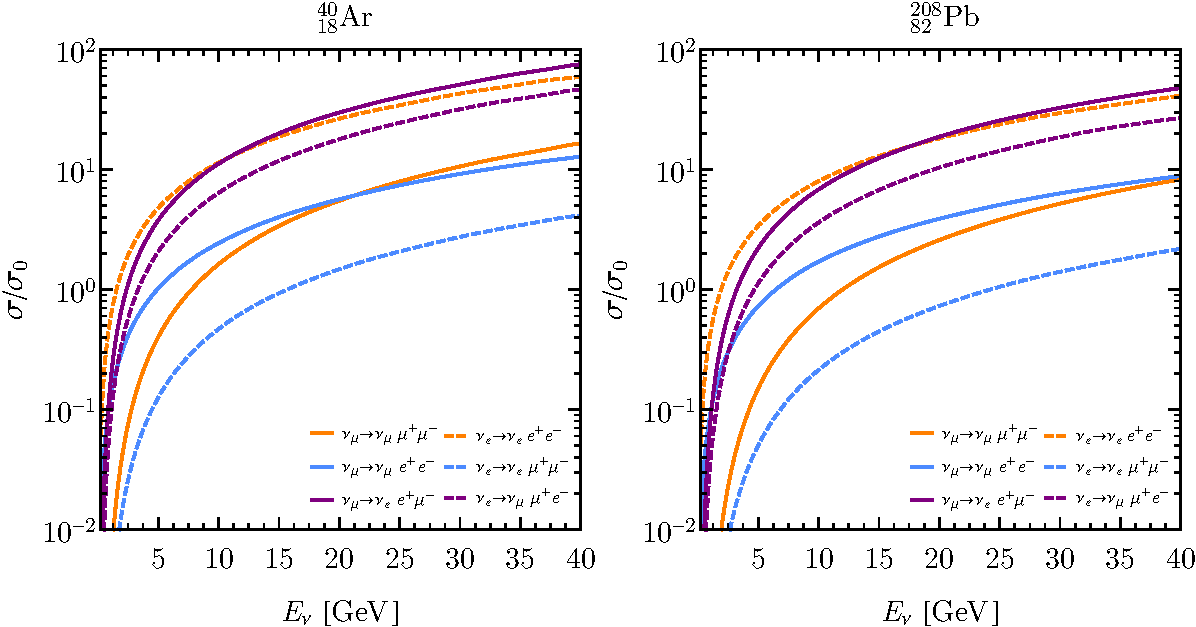
\includegraphics[width=\textwidth]{figs/Xsec_4PS_coh.pdf}
\caption[Coherent neutrino trident production total cross sections.]{Cross sections for coherent neutrino trident production on $^{40}$Ar (left) and  $^{208}$Pb (right) normalized to $\sigma_0 =  Z^2\, 10^{-44}$ cm$^2$. The full (dashed) lines correspond to the scattering of an incoming $\nu_\mu$ ($\nu_e$) produced by the NC (light-blue), CC (purple), and CC+NC (orange) SM interactions. \label{fig:coh_xsec}}
\end{figure}


%%%%%%%%%%%%%%%%%%%%%%%%%%%%%%%%%%%%%%%%%%%%%%%%%%%%
\subsubsection{Incoherent Regime ($\mathrm{H}^{\mu\nu}_\mathrm{d}$)}

At larger $Q^2$, the neutrino interacts with the individual nucleons of the nucleus. In this incoherent regime $\mathrm{H}^{\mu\nu}_\mathrm{d}$ is given by the sum of the contributions of the two types of nucleons: protons ($\mathrm{N=p}$) and neutrons ($\mathrm{N=n}$), so
\begin{equation}
\mathrm{H}^{\mu \nu}_\mathrm{d} (P, P^\prime) = Z\, \mathrm{H}^{\mu \nu}_\mathrm{p} (P, P^\prime)+
(A-Z)\,\mathrm{H}^{\mu \nu}_\mathrm{n}(P, P^\prime)\, ,
\end{equation}
where each $\mathrm{H}^{\mu \nu}_\mathrm{N}$ is the square of the matrix element of the nucleon electromagnetic current summed over final and averaged over initial spins. Neglecting second class currents, the matrix elements take the form
\begin{equation}
\bra{\mathrm{N}(P^\prime)} {J}^\mu_{\rm{E.M.}} (Q^2) \ket{\mathrm{N} (P) } = e \, \overline{u}_\mathrm{N} (P^\prime) \left[ \gamma^\mu F^\mathrm{N}_1(Q^2) - i \frac{\sigma^{\mu \nu} q_{\nu}}{2 M_{\rm N}} F^\mathrm{N}_2(Q^2) \right] u_\mathrm{N}(P)\, ,
\end{equation}
%
with $F^\mathrm{N}_{1,2}(Q^2)$ the Dirac and Pauli form factors, respectively. The hadronic tensors are then given by \cite{Kniehl:1990iv}
%
\begin{equation}
\mathrm{H}^{\mu \nu}_\mathrm{N} = e^2 \left[ 4 \, H_1^\mathrm{N}(Q^2) \left(P^\mu - \frac{q^\mu}{2}\right)\left(P^\nu - \frac{q^\nu}{2}\right) - H_2^\mathrm{N}(Q^2) \left( Q^2 g^{\mu \nu} + q^\mu q^\nu \right) \right]\, ,
\end{equation}
%
where the  $H_1^\mathrm{N}(Q^2)$ and $H_2^\mathrm{N}(Q^2)$ form factors, functions of $F^\mathrm{N}_{1,2}(Q^2)$, are given in Appendix~\ref{app:formfactors}. The flux functions in the incoherent regime can then be calculated as
\begin{subequations}\label{eq:dcoh}
\begin{align}
h^\mathrm{T}_\mathrm{N}(Q^2, \hat{s})  &=  8 \, e^2 \left[ \left(1 - \frac{\hat{s}}{2E_\nu M_{\rm N}} - \frac{\hat{s}^2}{4 E_\nu^2 Q^2 }\,\right) H_1^\mathrm{N}(Q^2) + \frac{\hat{s}^2}{8E_\nu^2 M_{\rm N}^2}  H_2^\mathrm{N}(Q^2)\right ]\, ,\label{eq:hTdiff}\\
%
h^\mathrm{L}_\mathrm{N}(Q^2, \hat{s})  &=  4 e^2 \, \left[ \left(1-\frac{\hat{s}}{4 E_\nu M_{\rm N}} \right)^2 H_1^\mathrm{N}(Q^2)  - \frac{\hat{s}^2}{16 E_\nu^2 M_{\rm N}^2} H_2^\mathrm{N}(Q^2)\right]\, .\label{eq:hLdiff}
\end{align}
\end{subequations}
%
In the case of the proton, the flux functions $h^{\rm T, L}_{\rm p}$ have some unique features given the presence of both electric and magnetic contributions. Specifically, the transverse function is non-zero at $Q=Q_{\rm min}$ for a fixed $\hat{s}$, due to the additional term proportional to $H_2^{\rm p}$. Indeed, for large values of $\hat{s}$, the $H_2^{\rm p}$ term dominates the transverse function. An opposite behaviour occurs for the longitudinal component. There, the $H_1^{\rm p}$ term dominates over the second term for all physical values of $\hat{s}$, $Q$, and for any incoming neutrino energy. On the other hand, the flux functions of the neutron, which have only 
the magnetic moment contribution, have somewhat different characteristics. While 
$h^{\rm T}_{\rm n}$ behaves similarly to $h^{\rm T}_{\rm p}$, that is, it is dominated by the second term for large values of $\hat{s}$, $h^{\rm L}_{\rm n}$ is zero at $Q_{\rm min}$ due to the exact cancellation between the $H_{1,2}^{\rm n}$ terms. This cancellation is not evident from Eq.\ ~\eqref{eq:hLdiff}; however, simplifying the longitudinal component for the neutron case, one finds
\begin{align*}
	h^\mathrm{L}_\mathrm{n}(Q^2, \hat{s})  &=4 e^2 \left(1+\frac{Q^2}{4M_{\rm n}^2}\right)\frac{Q^2}{4 M_{\rm N}^2}\left( 1 - \frac{\hat{s}}{2 E_\nu M_{\rm N}} - \frac{\hat{s}^2}{4 E_\nu^2 Q^2} \right) \left| F^\mathrm{n}_2(Q^2) \right|^2,
\end{align*}
which is zero for $Q=Q_{\rm min}$. Also, this shows why $h^{\rm L}_{\rm p}$ does not 
vanish at $Q_{\rm min}$ since there we have the additional contribution of the electric component. 

When the neutrino interacts with an individual nucleon inside the nucleus, one must be aware of the nuclear effects at play. One such effect is Pauli blocking, a suppression of neutrino-nucleon interactions due to the Pauli exclusion principle. Modelling the nucleus as an ideal Fermi gas of protons and neutrons, one can take Pauli blocking effects into account by requiring that the hit nucleon cannot be in a state which is already occupied \cite{Brown:1971qr}. This requirement is implemented in our calculations by a simple replacement of the differential incoherent cross section
\begin{align*}
\frac{\dd^2 \sigma_{\nu  \mathrm{d}}}{\dd Q^2 \dd \hat{s}}\to f (|\vec{q}|) \, \frac{\dd^2 \sigma_{\nu  \mathrm{d}}}{\dd Q^2 \dd \hat{s}},
\end{align*}
where $|\vec{q}|$ is the magnitude of the transferred three-momentum in the lab frame. In particular, following \cite{Brown:1971qr}, assuming an equal density of neutrons and protons, we have
%
\begin{equation}
f (|\vec{q}|) = \begin{cases} \displaystyle
                    \frac{3}{2} \frac{|\vec{q}|}{2 \, k_F} - \frac{1}{2} \left( \frac{|\vec{q}|}{2 \, k_F} \right)^3 ,\, &\mathrm{if }\;\; |\vec{q}| < 2\, k_F\, ,\\
                    1,\, &\mathrm{if }\;\; |\vec{q}| \geq 2 \, k_F\, ,
                \end{cases}
\end{equation}
%
where $k_F$ is the Fermi momentum of the gas, taken to be $235$ MeV. This is a rather low value of $k_F$ and the assumption of equal density of neutrons and protons must be taken with care for heavy nuclei. We refrain from trying to model any additional nuclear effects as we believe that this is the dominant effect on the total incoherent rate, particularly when requiring no hadronic activity in the event. The net result is a reduction of the incoherent cross section by about $50\%$ for protons and $20\%$ for neutrons. Unless clearly stated otherwise, we always include Pauli blocking in our calculations.

Our final cross sections for this regime can be seen in \reffig{fig:dif_xsec}. One can clearly see that the neutron contribution is subdominant, and that, up to factors of $Z^2$, the proton one is comparable to the coherent cross section. Note that now the typical values of $Q^2$ are much larger than in the coherent regime and the impact of the final-state lepton masses is much smaller. 

\begin{figure}[t]
\centering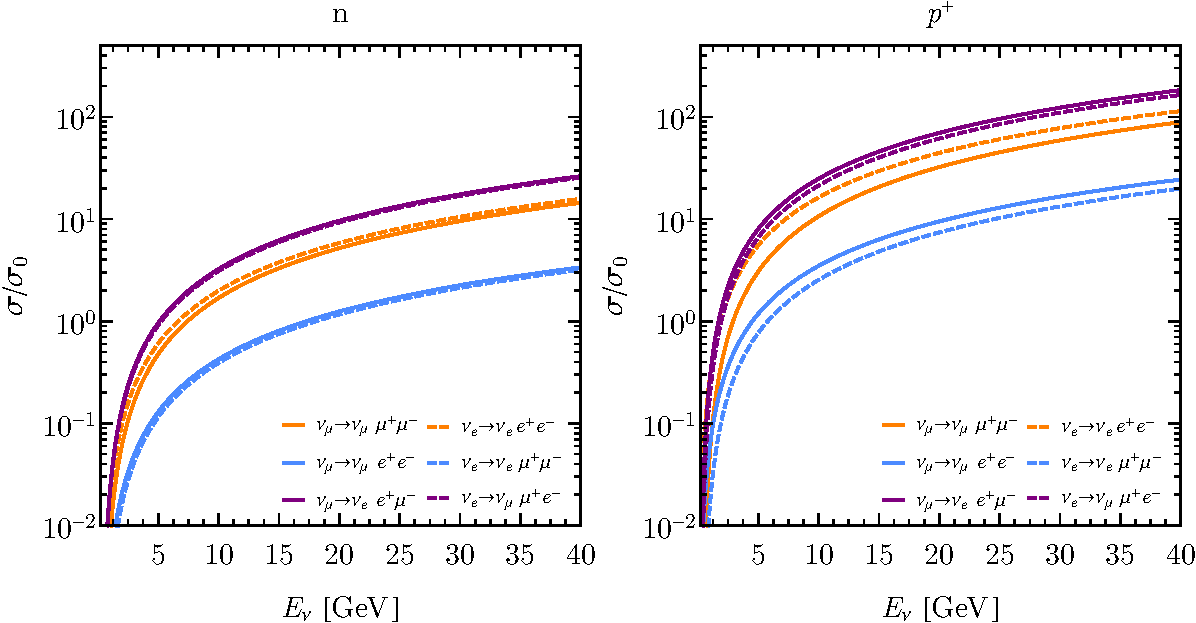
\includegraphics[width=\textwidth]{figs/Xsec_4PS_diff.pdf}
\caption[Incoherent neutrino trident production total cross sections.]{Cross sections for incoherent neutrino trident production on neutrons (left) and protons (right), including Pauli blocking effects as described in the text, normalized to $\sigma_0 =  10^{-44}$ cm$^2$. The full (dashed) lines correspond to the scattering of an incoming $\nu_\mu$ ($\nu_e$) produced by the NC (light-blue), CC (purple), and CC+NC (orange) SM interactions. \label{fig:dif_xsec}}
\end{figure}


%%%%%%%%%%%%%%%%%%%%%%%%%%%%%%%%%%%%%%%%%%%%%%%%%%%%
\subsection{Breakdown of the EPA \label{sec:EPAbreakdown}}

In order to understand the breakdown of the EPA in the neutrino trident case, let us first remind briefly the reader about the Weizs\"acker--Williams method of equivalent photons in Quantum Electrodynamics (QED)~\cite{vonWeizsacker:1934nji,Williams:1934ad}, and the main reason for its validity in that theory. The EPA, first introduced by E.\ Fermi~\cite{Fermi:1924tc}, is based on a simple principle: when an ultra-relativistic particle $P_i$ approaches a charged system $C_s$, like a nucleus, it will perceive the electromagnetic fields as nearly transverse, similar to the fields of a pulse of radiation, {\it i.e.},  as an on-shell photon. Therefore, it is possible to obtain an approximate total cross section for the inelastic scattering process producing a set of final particles $P_f$, $\sigma_{\rm t}(P_i + C_s \to P_f + C_s)$, by computing the scattering of the incoming particle with a real photon integrated over the energy spectrum of the off-shell photons,
%
\begin{align}
	\sigma_{\rm t}(P_i + C_s \to P_f + C_s)\approx\int\, dP(Q^2,\hat{s})\,\sigma_\gamma(P_i + \gamma \to P_f; \hat{s}, Q^2 = 0),
\end{align}
where the photo-production cross section for the process $P_i + \gamma \to P_f$, 
$\sigma_\gamma(P_i + \gamma \to P_f; \hat{s}, Q^2 = 0)$, 
depends on the center-of-mass energy of the $P_i$--photon system, $\sqrt{\hat{s}}$. Here $dP(Q^2,\hat{s})$ corresponds to the energy spectrum of the virtual photons, that is, the probability of emission of a virtual photon with transferred four-momentum $Q^2$ resulting in an center-of-mass energy $\sqrt{\hat{s}}$.
For trident scattering off a nuclear target, this probability can be approximated by~\cite{Belusevic:1987cw,Altmannshofer:2014pba}
\begin{align}\label{eq:GenEPA}
	dP(Q^2,\hat{s})=\frac{Z^2e^2}{4\pi^2}|F (Q^2)|^2\,\frac{d\hat{s}}{\hat{s}}\,\frac{dQ^2}{Q^2}\, .
\end{align}
A crucial fact in QED is that the cross section $\sigma_\gamma^{\rm QED}(P_i + \gamma \to P_f; \hat{s},0)$ is inversely proportional to $\hat{s}$,
\begin{align*}
	\sigma_\gamma^{\rm QED}(P_i + \gamma \to P_f; \hat{s},0) \propto \frac{1}{\hat{s}}\,.
\end{align*}
We see clearly that small values of $\hat{s}$ and consequently of the transferred four-momentum $Q^2$ dominate the cross section. Hence, the on-shell contribution is much more significant 
than the off-shell one, so the EPA will be valid and give the correct cross  section 
estimate for any QED process. 

Now, let us consider the case of neutrino trident production. In this case, the equivalent-photon cross section in the four-point interaction limit has a completely opposite dependence on the center-of-mass energy; it is \emph{proportional} to $\hat{s}$,
\begin{align*}
	\sigma_\gamma^{\rm FL}(P_i + \gamma \to P_f; \hat{s}, 0)\propto G_{\rm F}^2\, \hat{s}\, .
\end{align*}
This dependence is a manifestation of the unitarity violation in the Fermi theory. Therefore, we can see that for weak processes larger values of $\hat{s}$, and, consequently, larger values of $Q^2$ are more significant \cite{Kozhushner:1962aa, Shabalin:1963aa}.  The EPA is then generally not valid for the neutrino trident production, as the virtual photon contribution dominates over the real one. Nevertheless, one may wonder if there is a situation  in which the EPA can give a reasonable estimate for a neutrino trident process. 
As noticed in the early literature \cite{Kozhushner:1962aa, Shabalin:1963aa}, the presence of the nuclear form factor introduces a cut in the transferred momentum which, in turn, makes the EPA applicable for the specific case of the dimuon channel in the coherent regime. Let us discuss this in more detail. 

Recalling our exact decomposition, \refeq{eq:full_diff_xsec}, it is necessary to consider two assumptions for implementing the EPA \cite{Kozhushner:1962aa}:
%
\begin{enumerate} 
%
\item The longitudinal polarization contribution to the cross section can be neglected, i.e., $\sigma_{\nu\gamma}^\mathrm{L}(Q^2,\hat{s})\approx 0$;
%
\item The transverse polarization contribution to the cross section can be taken to be on-shell, i.e., $\sigma^\text{T}_{\nu\gamma}(Q^2,\hat{s}) \approx \sigma^\text{T}_{\nu\gamma}(0,\hat{s})$. 
%
\end{enumerate}
%
Assuming for now that these approximations hold, we can find a simplified expression for the coherent neutrino-target process, described by Eqs.~(\ref{eq:full_diff_xsec}) and (\ref{eq:hcoh}), in terms of the photon-neutrino cross section\footnote{An analogous expression can be obtained for the incoherent regime from Eq.~(\ref{eq:dcoh}).}:
%
\begin{align}     
\sigma_\text{EPA} = \frac{Z^2e^2}{4\pi^2}\int_{m_L^2}^{\hat{s}_{\rm max}} \frac{d\hat{s}}{\hat{s}}\,
\sigma^\mathrm{T}_{\nu\gamma}(0,\hat{s})
\int_{(\hat{s}/2E_\nu)^2}^{Q^2_{\rm max}}\frac{|F (Q^2)|^2}{Q^4} \left[ Q^2(1-y) - M_{\cal H}^2y^2\right]dQ^2\, , 
\end{align}
%
where we introduced the fractional change of the nucleus energy $y$, defined as $\hat{s} = (s-M_{\cal H}^2)y$, and the integration limits can be obtained from \eqref{eq:qslimts} after considering that $m_L^2\ll E_\nu M_{\cal H}$. Keeping only the leading terms in the small parameter $y$ \cite{Belusevic:1987cw}, we recover the EPA applied to the neutrino trident case
%
\begin{align} \label{eq:EPA_bad}
\sigma_\text{EPA} = \int \sigma^\mathrm{T}_{\nu\gamma}(0,\hat{s}) \, dP(Q^2,\hat{s})\, ,
\end{align}
%
where $dP(Q^2,\hat{s})$ is given in Eq.~(\ref{eq:GenEPA}). The EPA in the form of \refeq{eq:EPA_bad} has been used in trident calculations for the coherent dimuon channel \cite{Altmannshofer:2014pba} as well as for coherent mixed- and electron-flavour trident modes and incoherent trident modes \cite{Magill:2016hgc}.  Using our decomposition, we can explicitly compute both $\sigma^\mathrm{L}_{\nu \gamma}$ and $\sigma^\mathrm{T}_{\nu \gamma}$ and verify if the EPA conditions are satisfied for any channel and, if they are not, quantify the error introduced by making this approximation. For that purpose, we will compare the results of the full calculation, \refeq{eq:full_diff_xsec}, with the EPA results, \refeq{eq:EPA_bad}, by computing the following ratios in the physical region of the $(Q,\hat{s})$ plane,
\begin{align}\label{eq:ratios}
		\frac{\sigma^{\rm L}(Q^2,\hat{s})\,h_{\rm c}^{\rm L}(Q^2,\hat{s})}{\sigma^{\rm T}(Q^2,\hat{s})\,h_{\rm c}^{\rm T}(Q^2,\hat{s})}\, , \quad \frac{\sigma^\mathrm{T}_{\nu\gamma}(Q^2,\hat{s})}{\sigma^\mathrm{T}_{\nu\gamma}(0,\hat{s})}\, .
\end{align} 
The first ratio in Eq.\ \eqref{eq:ratios} will indicate where the longitudinal contribution can be neglected compared to the transverse one; while, the second ratio will show where the transverse contribution behaves as an on-shell photon. 

As an illustration of the general behaviour, we show in Fig.\ \ref{fig:4PSvsEPA} those ratios 
of cross sections for an incoming $\nu_\mu$ of fixed energy $E_\nu=3$ GeV colliding coherently with an $^{40}$Ar target, for the dielectron (left panels), mixed  (middle panels) and dimuon  (right panels)
channels. On the top panels of Fig.\ \ref{fig:4PSvsEPA} we see that the longitudinal component can be neglected for $Q\lesssim m_\alpha$, for the dielectron and dimuon channels, $\alpha=e,\mu$, while in the mixed case there is a much less pronounced hierarchy between the transverse and longitudinal components. On the bottom panels we have the comparison between on-shell and off-shell transverse photo-production cross sections. Again, we find that the EPA is only valid for $Q \lesssim m_\alpha$ for the dielectron and dimuon channels. For the mixed case, there is only a very small region in $Q < 10^{-2}$\,GeV for which the off-shell transverse cross section is comparable to the on-shell one. This relative suppression of the off-shell cross section can be understood by noticing that $Q$ enters the lepton propagators, suppressing the process for $Q \gtrsim m_\alpha$. For mixed channels it is then the smallest mass scale ($m_e$) that dictates the fall-off of the matrix element in $Q$, whilst the heaviest mass ($m_\mu$) defines the phase space boundaries, rendering most of this phase space incompatible with the EPA assumptions.   
%
\begin{figure}[t]
\centering
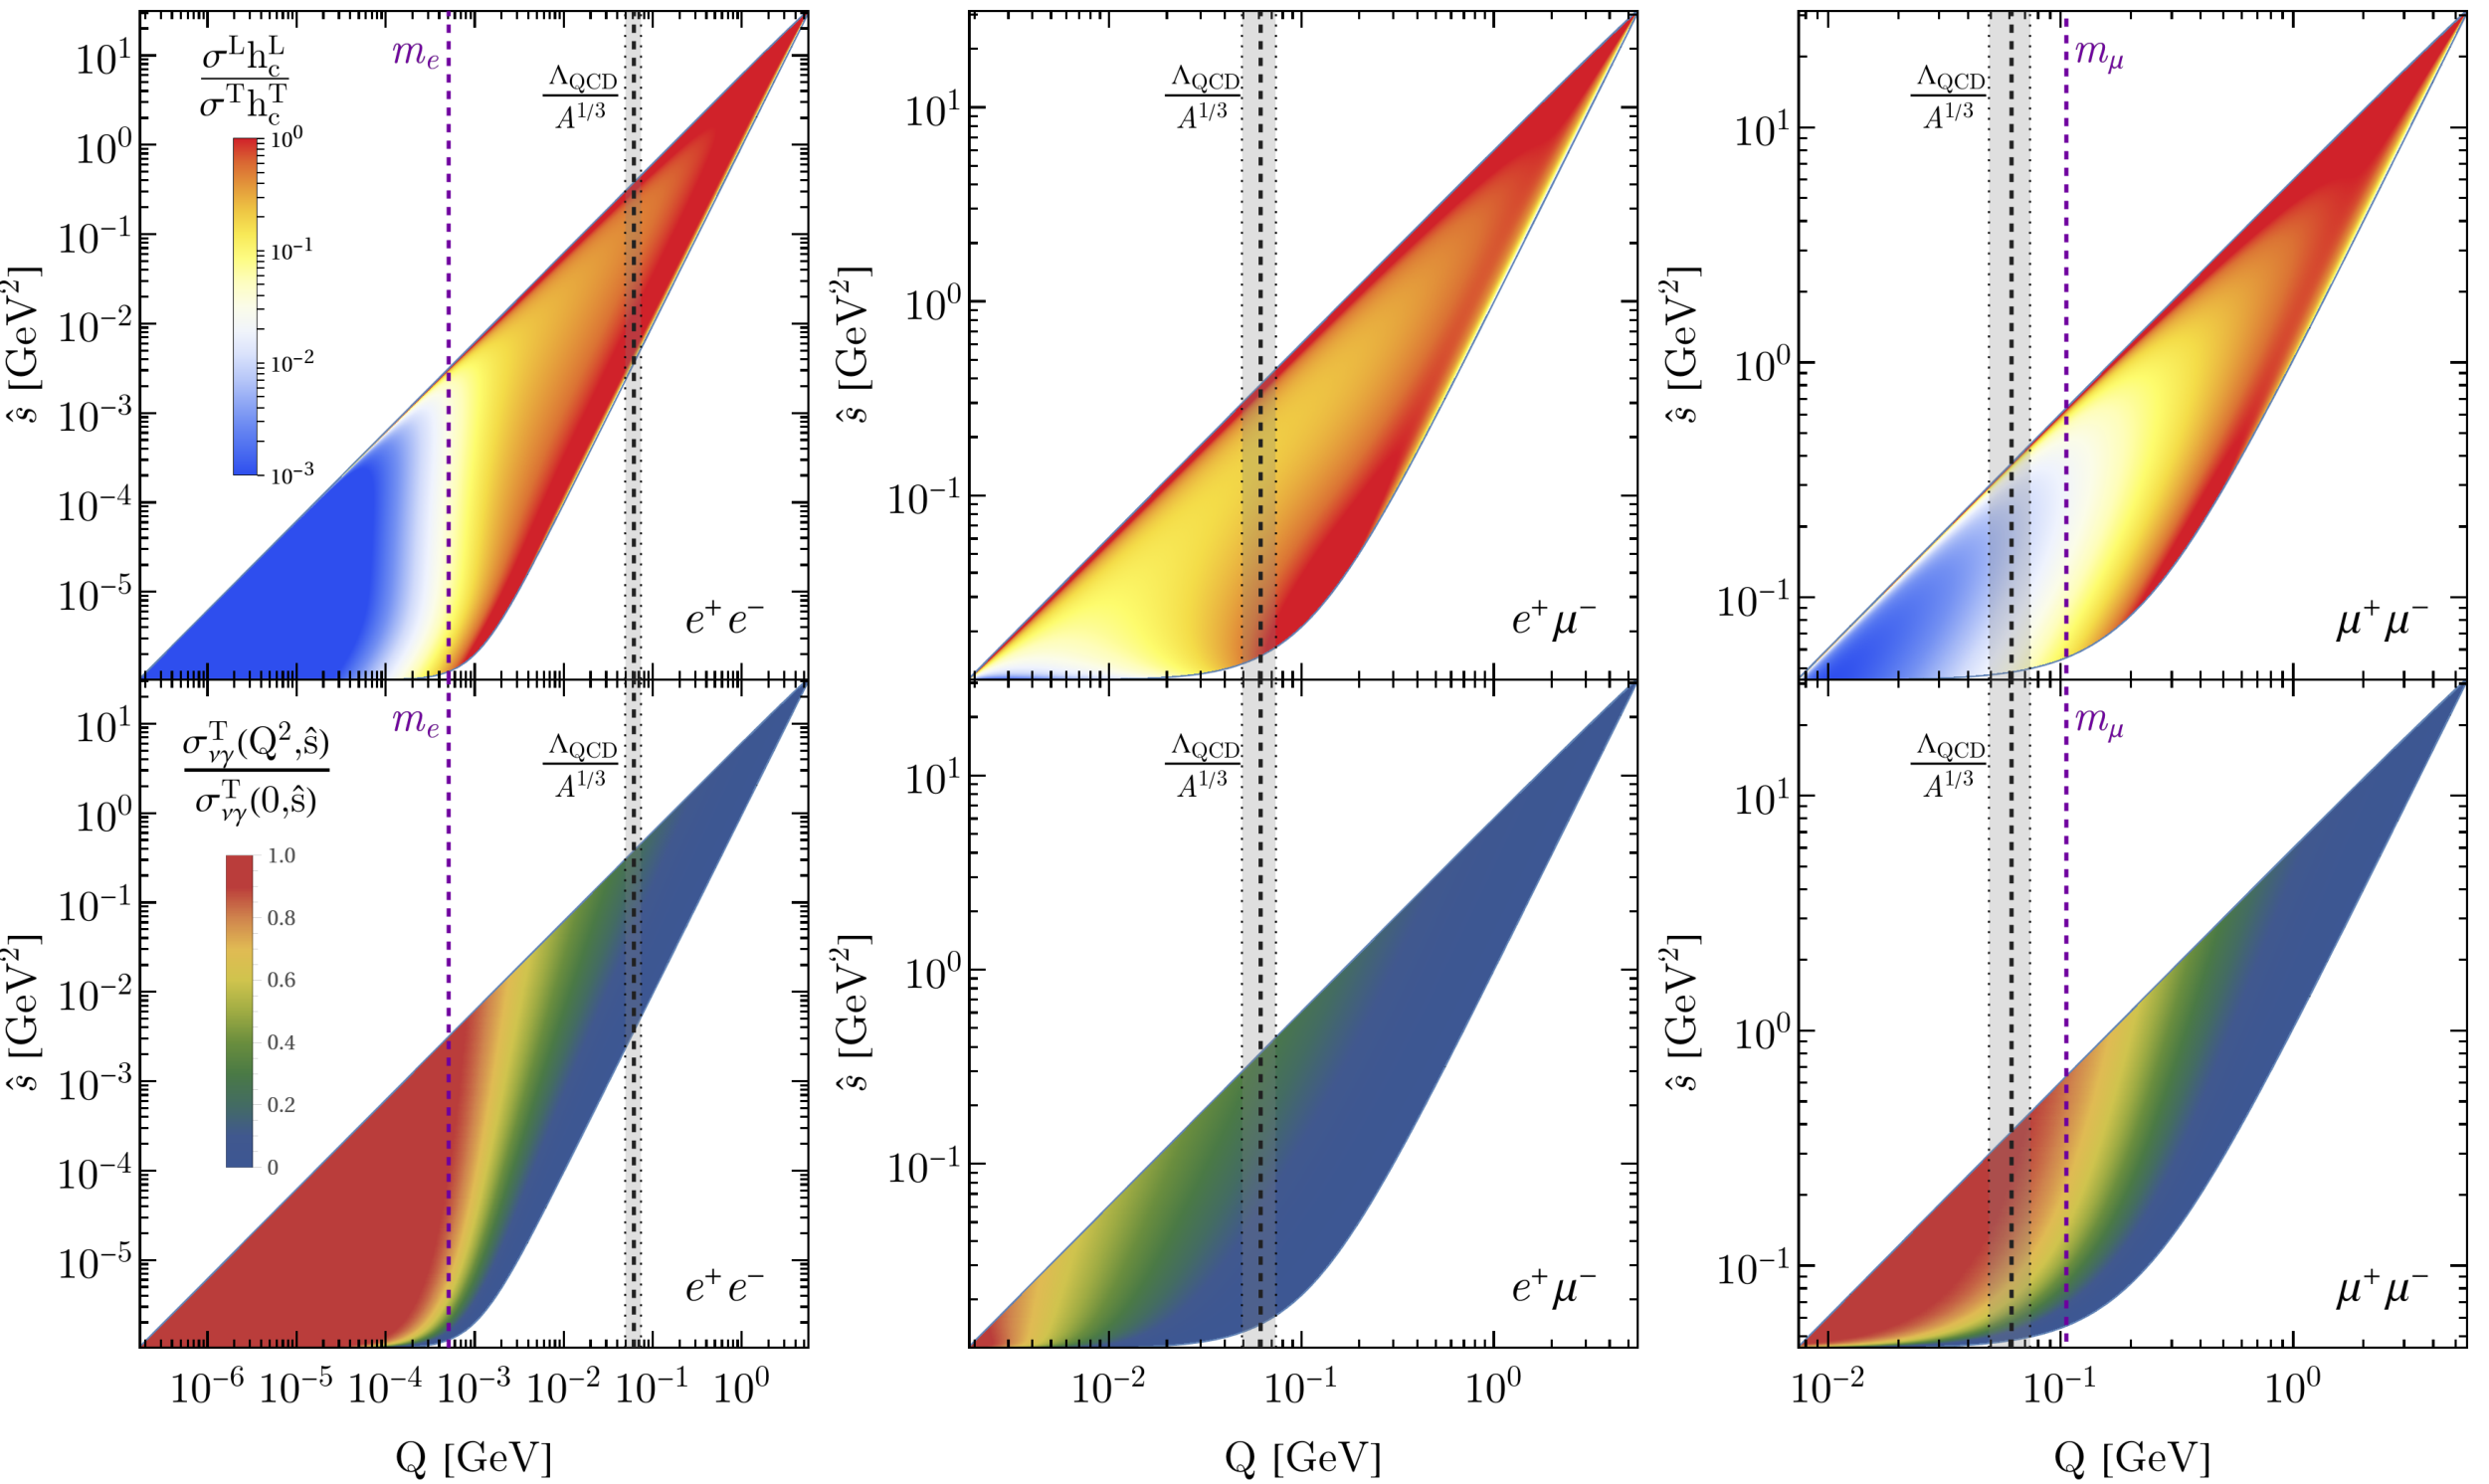
\includegraphics[width=\textwidth]{figs/4PS_vs_EPA.pdf}%
\caption[Comparison of the differential cross section using the EPA and using the full calculation for neutrino trident scattering.]{\label{fig:4PSvsEPA} Comparison between the full calculation of the trident production 
coherent cross section and the EPA in the kinematically allowed region of the $(Q,\hat{s})$ plane for an incoming $\nu_\mu$ with fixed energy $E_\nu=3$ GeV colliding with an $^{40}$Ar target. 
The left, middle and right panels correspond to the dielectron, mixed and dimuon final-states, respectively. The top panels correspond to the comparison between the longitudinal and transverse contributions while the bottom ones show the ratio between the transverse cross sections computed for an specific value of $Q$ with the cross section for an on-shell photon. The thick black dashed lines correspond to the cut in the $Q^2$ integration at $\Lambda_{\rm QCD}^2/ A^{2/3}$, and the shadowed region around these lines account for a variation of $20\%$ in the value of this cut. The purple dashed lines are for $Q=m_\alpha$, $\alpha=e,\mu$ for the unmixed cases.}
\end{figure}

These results explicitly show that the EPA is, in principle, not suitable for any neutrino trident process as it can overestimate the cross section quite substantially by treating the photo-production cross section at large $Q^2$ as on-shell. However, as previously mentioned, in the coherent regime the nuclear form factor introduces a strong suppression for large values of $Q^2$. In general, this dominates the behaviour of the cross sections for values of $Q^2$ smaller than the purely kinematic limit, $Q^2_{\rm max}$, and of the order of $\Lambda_{\rm QCD}/ A^{1/3}\approx 0.06$ GeV for coherent scattering on $^{40}$Ar. In the dimuon case, the latter scale happens to be smaller than the charged lepton masses, implying that the region where the EPA breaks down is heavily suppressed due to the nuclear form factor. The same cannot be said about coherent trident channels involving electrons, as the nuclear form factor suppression happens for much larger values of $Q$ than the EPA breakdown. Furthermore, for incoherent scattering the nucleon form factors suppress the cross sections only for much larger $Q$ values, $Q\approx 0.8$ GeV. The effective range of integration then includes a significant region where the EPA assumptions are invalid, leading to an overestimation of the incoherent cross section for every process regardless of the flavours of their final-state charged leptons. 

%
\begin{figure}[t]
	\centering
	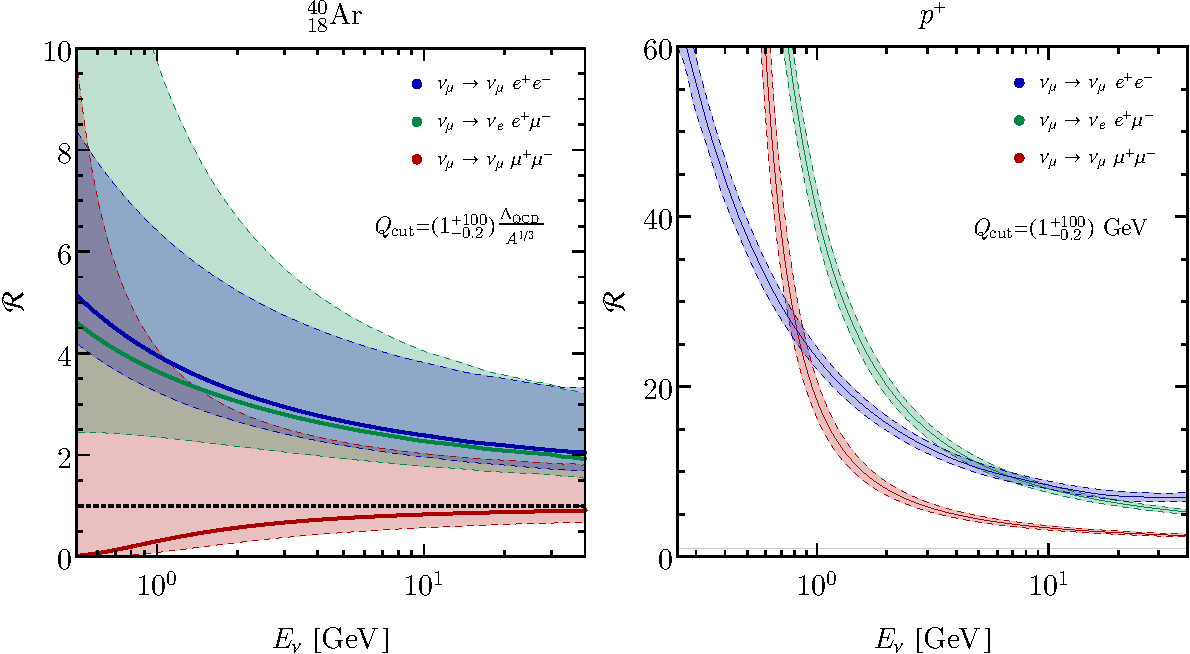
\includegraphics[width=\textwidth]{figs/XSec_ratio.pdf}%
	\caption[Comparison of the total cross section in the EPA and in the full calculation for neutrino trident scattering.]{\label{fig:comparison4PS_EPA} 
    Ratio $\mathcal{R}$ of the trident cross section calculated using 
    the EPA to the full four-body calculation. 
    Left panel: Ratio in the coherent regime on $^{40}$Ar. The full curves correspond to the central value of $Q_{\rm cut}$, and the upper (lower) boundary corresponds to a choice 100 times larger ($20\%$ smaller). 
Right  panel: Ratio in the incoherent regime for scattering on protons, where the full curves corresponds to the central value of $1.0$ GeV, and the upper (lower) boundary corresponds to a choice 100 times larger ($20\%$ smaller); we have taken the lower limit in the integration on $Q$ to match the choice of the coherent regime and we do not include Pauli blocking in these curves. A guide to the eye at $\mathcal{R} = 1$ is also shown.}
\end{figure}

In some calculations, artificial cuts have been imposed on the range of $Q^2$, affecting the validity of the EPA. In Ref. \cite{Magill:2016hgc}, it is claimed that to avoid double counting between different regimes, an artificial cut must be imposed, lowering the upper limit of integration in $Q^2$. Ref.~\cite{Magill:2016hgc} chooses a value of $Q^{\rm cut}_{\rm max} = \Lambda_{\rm QCD}/ A^{1/3}$ in the coherent regime (black thick dashed lines in Fig.\ \ref{fig:4PSvsEPA}), and $Q^{\rm cut}_{\rm min}= {\rm max}\left( \Lambda_{\rm QCD}/ A^{1/3}, \hat{s}/2E_\nu\right)$ and $Q^{\rm cut}_{\rm max} = 1.0$ GeV in the incoherent regime. We believe that no such cut is required on physical grounds\footnote{It should be noted that the coherent and incoherent regimes have different phase space boundaries and that the form factors should guarantee their independence.}, and their presence will impact the EPA cross section quite dramatically. Let us first consider the dimuon case in the coherent regime, where the EPA assumptions hold reasonably well in the relevant parts of phase space. By introducing a value for $Q^{\rm cut}_{\rm max}$ we would be decreasing the total relevant phase space for the process, reducing the total cross section. Therefore, despite the EPA tendency to overestimate the cross section in this channel, an artificial cut in $Q^2$ can actually lead to an underestimation of the cross section. In the electron channels, where the EPA breakdown is much more dramatic, we can expect that the overestimation of the cross section by the EPA is reduced by the cut $Q^{\rm cut}_{\rm max}$. In fact, one way to improve the EPA for the dielectron channel is to artificially cut on the $Q^2$ integral around the region where the ap\-pro\-xi\-ma\-tion breaks down \cite{Frixione:1993yw}. This cut does then improve the coherent EPA calculation by decreasing the overestimation of the cross section. However, an energy independent cut cannot provide a good estimate of the cross section over all values of $E_\nu$. To illustrate our point and to quantify the errors induced by the EPA, we show on the left panel of \reffig{fig:comparison4PS_EPA} the ratio $\mathcal{R}$ of the trident cross section calculated using the EPA with an artificial cut at $Q^2_\text{cut}$, as performed in \cite{Magill:2016hgc}, to the full calculation used in this work as a function of the incoming neutrino energy:
%
 \begin{equation}
 \mathcal{R} = \frac{\sigma_{\rm EPA} (E_\nu) \vert_{Q_{\rm cut}}}{\sigma_{\rm 4PS} (E_\nu)}\,.
 \end{equation}
%
 In this plot we vary the artificial cut on $Q^2$ around the choice of \cite{Magill:2016hgc} (shown as the central dashed line) in two ways. First we reduce it by $20 \%$, and then increase it by a large factor, recovering the case with no $Q^2$ cut. From this, our conclusions about the validity of the approximation are confirmed, and it becomes evident that the trident coherent cross section is very sensitive to the choice of $Q^2_{\mathrm{cut}}$. In particular, the EPA with all the assumptions that lead to \refeq{eq:EPA_bad} and the absence of a $Q^2$ cut can lead to an overestimation of all trident channels, including the dimuon one. Once the cut is implemented, however, the approximation becomes better for the dimuon channel, but still unacceptable for the electron ones. It is also clear that an energy independent cut cannot give the correct cross section at all energies. This is particularly troublesome for detectors subjected to a neutrino flux covering a wide energy range such as the near detectors for DUNE and  MINOS or MINER$\nu$A. Moreover, \refeq{eq:EPA_bad} fails at low energies, and generally, overestimates the coherent cross sections by at least  200\%. At these energies, one must be wary of the additional approximations in \refeq{eq:EPA_bad} regarding the integration limits and the small $y$ limit.     

On the right panel of \reffig{fig:comparison4PS_EPA} we illustrate what happens in the incoherent regime, where the nucleon form factors impact the cross section at much larger values of $Q^2$ and have a slower fall-off. We see that the incoherent cross section is dramatically overestimated over the full range of $E_\nu$ considered and for any trident mode. The discrepancy is particularly important for $E_\nu \lesssim$ 5 GeV and larger than in the coherent regime by at least an order of magnitude\footnote{There are some differences in the treatment of the hadronic system between the EPA calculation in \cite{Magill:2016hgc} and the one presented here. However, these differences are of the order 10\% to 20\%. Note also that we do not implement any Pauli blocking when calculating $\mathcal{R}$ to avoid ambiguities over the choice of the range of $Q^2$.}. We also see that the cuts on $Q^2$ impact the EPA calculation much less dramatically, and that its use is unlikely to yield the correct result.

Given these problems with both coherent and incoherent cross section calculations due to the breakdown of the EPA for trident production, in what follows we will use the complete four-body calculation.

%%%%%%%%%%%%%%%%%%%%%%%%%%%%%%%%%%%%%%%%%%%%%%%%%%%%
\subsection{Coherent versus incoherent Scattering in Trident Production}
\label{subsec:cohdiff}

%
\begin{figure}[t]
	\centering
	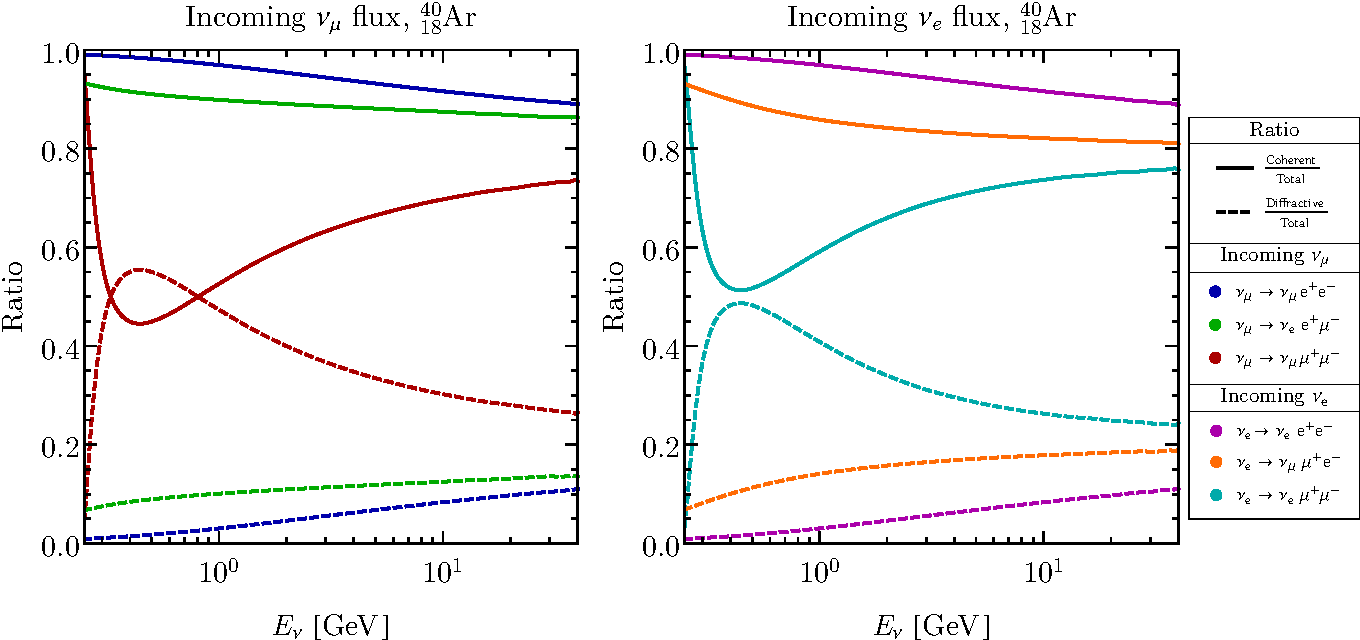
\includegraphics[width=\textwidth]{figs/Ratio_CDvsT.pdf}%
	\caption[Ration between coherent and incoherent trident total cross sections.]{\label{fig:RatioCDvsT} On the left (right) panel we show the
    ratio of the coherent (full lines) and the incoherent (dashed lines) contributions to the total trident cross section for an incoming flux of $\nu_\mu$($\nu_e$) as a function of $E_\nu$ for an 
    $^{40}$Ar target.}
\end{figure}
%

Let us  now comment on the significance of  the coherent and incoherent contributions to the total cross for the different trident channels. 
In Fig.\ \ref{fig:RatioCDvsT} we present the ratio of the coherent and the incoherent scattering cross sections to the total cross section for an $^{40}$Ar target for an incoming $\nu_\mu$ (left) and $\nu_e$ (right)  neutrino. We can see that the coherent regime dominates at all neutrino energies when there is an electron in the final-state, especially in the dielectron case. 
This can be explained by noting that the $Q^2$ necessary to create an electron pair is smaller than the one needed to create a muon; thus, coherent scattering is more likely to occur for this mode. Conversely, 
as one needs larger momentum transferred to produce a muon (either accompanied by an electron 
or another muon) the  incoherent regime becomes more likely in these modes, as we can explicitly 
see in Fig.\ \ref{fig:RatioCDvsT}. 
Because of this effect the incoherent contribution is $\lesssim$ 10\%, except for the 
dimuon channel where it can be between $30$ and $40$\% in most of the energy region.
Furthermore, when we compare the two incoming types of neutrinos, we see that for an incoming $\nu_\mu$ the incoherent contribution is larger than the coherent one in the range $0.3\ {\rm GeV}\lesssim E_\nu \lesssim 0.8$ GeV, while for an incoming $\nu_e$ this never happens. 
This difference can be explained by the fact that CC and NC contributions  are simultaneously present for the scattering of an initial $\nu_\mu$ creating a muon pair, whereas
for an initial $\nu_e$ creating a muon pair, we will only have the NC contribution, see Table \ref{tab:tridentmodes}.

An important difference between the coherent and incoherent regimes will be in their hadronic signatures in the detector. Neutrino trident production is usually associated with zero hadronic energy at the vertex, a feature that proved very useful in reducing backgrounds in previous measurements. Whilst this is a natural assumption for the coherent regime, it need not be the case in the incoherent one. In fact, in the latter it is likely that the struck nucleon is ejected from the nucleus in a significant fraction of events with $Q$ exceeding the nuclear binding energy
%
\footnote{The peak of our incoherent $Q^2$ distributions happens at around $Q \approx 300$ MeV, much beyond the typical binding energy for Ar (see \refapp{app:distributions}). Without Pauli suppression, however, we expect this value to drop.}. Since the dominant incoherent contribution comes from scattering on protons, these could then be visible in the detector if their energies are above threshold. On the other hand, the struck nucleon is subject to many nuclear effects which may significantly affect the hadronic signature, such as interactions of the struck nucleon in the nuclear medium as well as reabsorption. Our calculation of Pauli blocking, for example, shows large suppressions ($\sim 50\%$) precisely in the low $Q^2$ region, usually associated with no hadronic activity. This then raises the question of how well one can predict the hadronic signatures of incoherent events given the difficulty in modelling the nuclear environment. We therefore do not commit to an estimate of the number of incoherent events that would have a coherent-like hadronic signature, but merely point out that this might introduce additional uncertainties in the calculation, especially in the $\mu^+ \mu^-$ channel where the incoherent contribution is comparable to the coherent one. Finally, from now on we will refer to the number of trident events with no hadronic activity as coherent-like, where this number can range from coherent only to coherent plus all incoherent events. 


%%%%%%%%%%%%%%%%%%%%%%%%%%%%%%%%%%%%%%%%%%%%%%%%%%%%
\section{Trident Events in LAr Detectors}
\label{sec:LAr}

In this section we calculate the total number of expected  trident events for some present and future LAr detectors with different fiducial masses, total exposures and beamlines. In Table~\ref{tab:LAr} we specify the values used for each set-up and in Fig.~\ref{fig:LAr} we show the total production cross section for each neutrino trident mode of Table~\ref{tab:tridentmodes}
as well as the neutrino fluxes as a function of $E_\nu$ at the position of each experiment.  

%%%%%%%%%%%%%%%%%%%%%%%%%%%%%%%%%%%%%%%%%%%%%%%%%%%%
\subsection{Event Rates}
\label{subsec:rates}

The total number of trident events, $N^{\text{\Neptune}}_{\rm X}$, expected for a given trident mode at any detector is written as  
\begin{eqnarray}
\label{eq:nevents}
N^{\text{\Neptune}}_{\rm X}={\rm Norm}\times\int dE_\nu \, \sigma_{\nu {\rm X}}(E_\nu) \frac{d\phi_{\nu}(E_\nu)}{dE_\nu}\epsilon(E_\nu)\,,
\end{eqnarray}
where $\sigma_{\nu {\rm X}}$ can be the trident total (${\rm X}={\cal N}$), coherent ($\mathrm{X=c}$) or incoherent ($\mathrm{X=d}$) cross sections 
for a given mode, $\phi_{\nu}$ is the flux of the incoming neutrino and $\epsilon(E_\nu)$ is the efficiency of detection of the charged leptons. In the calculations of this section, we assume an efficiency of $100\%$\footnote{See \refsec{subsec:kine} for a discussion on the detection efficiencies for trident events and backgrounds.}.
%
The normalization is calculated as 
 %
$${\rm Norm}= {\rm{Exposure}}~[{\rm{POT}}] \times \frac{{\rm{Fiducial~Detector~Mass}\times N_A}}{m_{\rm T}} \left[{\rm{target~particles}}\right],$$
%%
where $m_{\rm T}$ is the molar mass of the target particle and $N_A$ is Avogadro's number.
%
Two features of the cross sections are important for the event rate calculation: 
threshold effects, especially for channels involving muons in the final-state,
and cross section's growth with energy. In particular, we expect higher trident event rates for experiments with higher energy neutrino beams. 

We start our study with the three detectors of the SBN program, one of which, $\mu$BooNE, is already installed and taking data at Fermilab. These three LAr time projection chamber detectors are located along the Booster Neutrino Beam line which is by now a well-understood source, having the focus of active research for over 15 years. 
%
Although the number of trident events expected in these detectors is rather low, they may offer one of the first opportunities to study trident events in LAr, as well as to better understand their backgrounds in this medium and to devise improved analysis techniques.
%
After that we study the proposed near detector for DUNE. This turns out to be the most important LAr detector for trident production since it will provide the highest number of events in both neutrino and antineutrino modes. 
%
Finally, having in mind the novel flavour composition of neutrino beams from muon facilities, we investigate trident rates at a 100~t LAr detector for the $\nu$STORM project. This last facility could offer a very well understood neutrino beam with as many electron neutrinos as muon antineutrinos from muon decays, creating new possibilities for trident scattering measurements.
%%
\begin{table}[t]
\begin{center}
\scalebox{0.9}{
\begin{tabular}{|cccccc|}
\hline\hline
		\bf Channel & \bf SBND& \bf $\mu$BooNE & \bf ICARUS & \bf DUNE ND &\bf  $\nu$STORM ND \\ \hline \hline
		$\nu_\mu\to\nu_e e^+ \mu^-$& $10$ &$0.7$ &$1$ &$2844 ~ (235)$ & $159$ \\
        &$1$ &$0.08$ &$0.1$ &$369 ~ (33)$& $18$\\\hline
        $\overline\nu_\mu\to\overline\nu_e e^- \mu^+$&$0.4$ &$0.02$ &$0.04$ &$122~(2051)$ & $23$\\
        &$0.04$ &$0.003$ &$0.004$ &$16~(262)$ & $3$\\\hline
	$\nu_e\to\nu_\mu e^- \mu^+$& $0.05$ &$0.003$ &$0.004$ &$22~(7)$ & $9$\\
        &$0.008$ &$0.0005$ &$0.0008$ &$5~(1)$ & $2$\\\hline
	$\overline\nu_e\to\overline\nu_\mu e^+ \mu^-$& $0.005$ &$0.0003$ &$0.0005$ &$5~(14)$ & $-$\\
    &$0.001$ &$0.0001$ &$0.0001$ &$1~(3)$ & $-$\\\hline
    \hline\hline
    {$\rm{Total} \ e^\pm \mu^\mp$}& $10$ &$0.7$ &$1$ &$2993~(2307)$ & $191$ \\
    &$1$ &$0.1$ &$0.1$ &$391~(299)$ & $23$\\\hline
    \hline
		$\nu_\mu\to\nu_\mu e^+ e^-$& $6$ &$0.4$ &$0.7$ &$913~(58)$ & $73$ \\
        &$0.2$ &$0.04$ &$0.02$ &$57~(5)$ & $3$\\\hline
        $\overline\nu_\mu\to\overline\nu_\mu e^- e^+$& $0.2$ &$0.01$ &$0.02$ &$34~(695)$ & $9$\\
        &$0.01$ &$0.001$ &$0.002$ &$2~(41)$ & $0.5$\\\hline
	$\nu_e\to\nu_e e^- e^+$&$0.2$ &$0.01$ &$0.02$ &$50~(13)$ & $32$ \\
    &$0.01$ &$0.001$ &$0.002$ &$4~(1)$ & $2$\\\hline
	$\overline\nu_e\to\overline\nu_e e^+ e^-$&$0.02$ &$0.001$ &$0.002$ &$10~(34)$ & $-$ \\
    &$0.0009$ &$0.0001$ &$0.0002$ &$1~(2)$ & $-$\\\hline
    \hline\hline
    ${\rm{Total}}\  e^+ e^-$& $6$ &$0.4$ &$0.7$ &$1007~(800)$ & $114$\\
    &$0.2$ &$0.0$ &$0.02$ &$64~(49)$ & $6$\\\hline
    \hline    
		$\nu_\mu\to\nu_\mu \mu^+ \mu^-$& $0.4$ &$0.03$ &$0.04$ &$271~(32)$ & $9$ \\
        &$0.3$ &$0.03$ &$0.04$ &$135~(14)$ & $5$\\\hline
        $\overline\nu_\mu\to\overline\nu_\mu \mu^- \mu^+$& $0.01$ &$0.001$ &$0.001$ &$14~(177)$ & $2$\\
        &$0.01$ &$0.0009$ &$0.001$ &$7~(93)$ & $1$\\\hline
 $\nu_e\to\nu_e \mu^+ \mu^-$    &$0.002$ &$0.0001$ &$0.0001$ &$1~(0.5)$ & $0.4$\\  
 &$0.001$ &$0.0001$ &$0.0001$ &$0.5~(0.2)$ & $0.2$\\\hline
        $\overline\nu_e\to\overline\nu_e \mu^+ \mu^-$&$0.0002$ &$0.0000$ &$0.0000$ &$0.3~(0.9)$ & $-$\\
        &$0.0001$ &$0.0000$ &$0.0000$ &$0.1~(0.3)$ & $-$\\\hline
        \hline\hline
    ${\rm{Total}} \ \mu^+ \mu^-$ &$0.4$ &$0.0$ &$0.0$ &$286~(210)$ & $11$ \\
    &$0.3$ &$0.0$ &$0.0$ &$143~(108)$ & $6$\\
    \hline\hline
\end{tabular}}
\end{center}
\caption[Trident rates in LAr detectors.]{\label{tab:LArrates}Total number of \textbf{coherent} (top row) and \textbf{incoherent} (bottom row) trident events expected at different LAr experiments for a given channel.
The numbers in parentheses are for the antineutrino running mode, when present. These calculations  
considered a detector efficiency of 100\%. }
\end{table}
%%%%%%%%%%%%%%%%%%%%%%%%%%%%%%%%%%%%%%%%%%%%%%%%%%%%
\paragraph{The SBN Program}

The SBN Program at Fermilab is a joint endeavour by three collaborations ICARUS, $\mu$BooNE and 
SBND to perform searches for eV-sterile neutrinos and study neutrino-Ar cross sections \cite{SBNproposal}. As can be seen in Tab.~\ref{tab:LAr}, SBND has the shortest baseline (110 m) and therefore the largest neutrino fluxes (shown in Fig.~\ref{fig:LAr} and taken from Fig. 3 of \cite{SBNproposal}). The largest detector, ICARUS, is also the one with the longest baseline (600 m) and consequently subject to the lowest neutrino fluxes.
%
The ratio between the fluxes at the different detectors are  $\phi_{\mu\rm{BooNE}}/\phi_{\rm{SBND}}=5$\% and $\phi_{\rm{ICARUS}}/\phi_{\rm{SBND}}=3$\%.
%
The neutrino beam composition is about 93\% of $\nu_\mu$,  6\% of $\overline\nu_\mu$ and  
$1\%$ of $\nu_e+\overline{\nu}_e$. 

Considering the difference in fluxes and the total number of targets in each of these 
detectors, one can estimate the following ratios of trident events: 
${N^\text{\Neptune}_{\mu\rm{BooNE}}}/{N^\text{\Neptune}_{\rm{SBND}}}\sim 8$\% and ${N^\text{\Neptune}_{\rm{ICARUS}}}/{N^\text{\Neptune}_{\rm{SBND}}}\sim 10$\%. Unfortunately, 
since the fluxes are peaked at a rather low energy ($E_\nu \lesssim 1$ GeV), where the trident  
cross sections are still quite small ($\lesssim 10^{-42}$ cm$^2$) we expect very few 
trident events produced.
%
The exact number of trident events for those detectors according to our calculations is 
presented in Tab.~\ref{tab:LArrates}. For each trident channel the first (second) row
shows the number of coherent (incoherent) events. As expected, less than a total 
of 20 events across all channels can be detected by SBND, and a negligible rate of events is expected at $\mu$BooNE and ICARUS. 

%%%%%%%%%%%%%%%%%%%%%%%%%%%%%%%%%%%%%%%%%%%%%%%%%%%%
\paragraph{DUNE Near Detector} The DUNE experiment will operate with neutrino as well as antineutrino LBNF beams produced by 
directing a 1.2 MW beam of protons onto a fixed target \cite{Acciarri:2016ooe,DUNECDRvolII}. 
The design of the near detector is not finalised, but the current designs favour a mixed technology  detector combining a LAr TPC with a larger tracker module.  In this work, we will assume that DUNE ND is a LAr detector located at $574$ m from the target with a fiducial mass of 50~t \cite{WeberTalk}. As the trident event rate scales with the density of the target, any tracker module will not significantly influence the total event rate, and does not feature in our estimates; although, its presence is assumed to improve reconstruction of final-state muons. Our estimates can be easily scaled for the final design by using \refeq{eq:nevents}.

For the first 6 years of data taking (3 years in the neutrino plus 3 years in the antineutrino 
mode) the collaboration expects $1.83\times 10^{21}$~POT/year with  a plan to upgrade the beam after the 6th year for 2 extra years in each beam mode  with double exposure, making a total of $1.83 \times(3+2\times2)\times 10^{21}~{\rm{POT}}$ for each mode \cite{DUNE:exposure}. We will 
assume the total 10-year exposure in our calculations.
%
. as the relevant fluxes at the DUNE ND location (see Fig.~\ref{fig:LAr}). The beam composition of the neutrino (antineutrino) beam is about 96\% $\nu_\mu$ ($\overline\nu_\mu$), 4\%  $\overline\nu_\mu$ ($\nu_\mu$) and 1\% $\nu_e+\overline\nu_e$.
 
The number of trident events for DUNE ND can be found in Tab.~\ref{tab:LArrates}. 
The numbers in parentheses correspond to antineutrino beam mode.
Note that although the trident cross sections are the same 
for neutrinos and antineutrinos, the fluxes are a bit lower for the antineutrino beam, as a consequence we predict a lower event rate for this beam\footnote{A similar difference will apply to the processes constituting the background to the trident process, although there is an additional suppression in many channels due to the lower antineutrino cross sections.}.
%
Due to the much higher energy and wider energy range of the neutrino fluxes at DUNE ND, as compared to the SBN detectors, DUNE can observe a considerable number of trident events, about 300 times the number of trident events expected for SBND just in the neutrino mode. Moreover, the subdominant component of 
each beam mode will also contribute to the signal. For example, we expect to observe $2051$ trident events in the $\overline{\nu}_\mu\to\overline{\nu}_e e^- \mu^+$ channel in the antineutrino mode. However, we also expect 
$235$ events in the $\nu_\mu\to\nu_e e^+ \mu^-$ channel produced by 
the subdominant component of $\nu_\mu$ in the antineutrino beam.
%
We have considered 100\% detection efficiency here, however, we will see in Sec.~\ref{subsec:bck} that after implementing hadronic vetos, detector thresholds and kinematical cuts to substantially reduce the background we expect an efficiency of about 47\%-65\% on coherent tridents, depending on the channel (see Tab.~\ref{tab:DUNE_ND_NU_BG}).

The mixed flavour trident channel is the one with the highest statistics (more than 6000 events adding 
neutrino and antineutrino beam modes), 11\% of which are produced by incoherent scattering. The dielectron channel comes next with a total of a bit more than 1900 events, 5\%  of which are produced by incoherent scattering. Although the  dimuon channel is the less copious one, with only about 
750 events produced, almost 34\% of these events are produced by a incoherent process.
This can be understood by recalling our discussions in Sec.~\ref{subsec:cohdiff}.

Finally, we note that a dedicated high-energy run at DUNE has been mooted, to be undertaken after the full period of data collecting for the oscillation analysis. Thanks to the higher energies of the beam, this has the potential to see a significant number of neutrino tridents, provided it can collect enough POTs.  

%%%%%%%%%%%%%%%%%%%%%%%%%%%%%%%%%%%%%%%%%%%%%%%%%%%%
\paragraph{$\nu$STORM} In this section we study the trident rates for a possible LAr detector for the proposed 
$\nu$STORM experiment \cite{Soler:2015ada,nuSTORM2017}. The $\nu$STORM facility 
is based on a neutrino factory-like design and has the goal to search for sterile neutrinos and study neutrino nucleus cross sections \cite{Adey:2014rfv}. Although this proposal is in its early days, $\nu$STORM has the potential to make cross section measurements with unprecedented precision. In its current design, $120$-GeV protons are used to produce pions from a fixed target with the pions subsequently decaying into muons and neutrinos. The muons are captured in a storage ring and during repeated passes around the ring they decay to produce neutrinos.
%
Consequently, the storage ring is an intense source of three types of neutrino
flavours: $\nu_\mu$ from $\pi^+$ and $K^+$ decays, which will be more than $99\%$ of the total flux, $\nu_e$ and $\overline\nu_\mu$ from recirculated muon decays which will comprise less than $1\%$ of the total flux. An important point, however, is that the neutrinos coming from the pion and kaon decays can be separated by event timing from the ones produced by the stored muons. This distinction allows the $\nu_\mu$ flux to be studied almost independently from the $\overline{\nu}_\mu$ and $\nu_e$ flux. In addition, it implies after the initial flash of meson-derived events, that the flux consists of as many electron neutrinos as muon antineutrinos. We will assume a LAr detector for $\nu$STORM at a baseline of 50\,m with 100\,t of fiducial mass with an exposure of $10^{21}$ POT. The neutrino fluxes, assuming 
a central $\mu^+$ momentum of $3.8$~GeV/c in the storage ring, are taken from Ref.~\cite{nuSTORM2017} and are 
shown in Fig.~\ref{fig:LAr}.

In Tab.~\ref{tab:LArrates}, we show the results of our calculations for $\nu$STORM. 
More than $97\%$ of the events from the incoming $\nu_\mu$ are from pion decays and only less 
than $3\%$ from kaon decays. Since we only consider the decay of mesons with positive charges and we expect neutral and wrong charge contamination to be small, we do not have trident events from incoming $\overline\nu_e$.
%
The total number of mixed flavour, dielectron and dimuon channel events is, respectively,
214, 120 and 17, much less than what can be achieved at the larger neutrino energies available at the DUNE ND. The novel flavour structure of the beam does enhance the contribution of $\nu_e$ induced tridents with respect to the $\pbar{\nu}_\mu$ ones, but this contribution only becomes dominant for the $e^+e^-$ tridents in the muon decay events. Finally, we emphasize that the experimental design parameters for $\nu$STORM are far from definite. Increasing the energy of stored muons and the size of the detector are both viable options which could significantly enhance the rates we present.

%

%%%%%%%%%%%%%%%%%%%%%%%%%%%%%%%%%%%%%%%%%%%%%%%%%%%%
\subsection{Background Estimates for Neutrino Trident in LAr}
\label{subsec:bck}

The study of any rare process is a struggle against both systematic uncertainties in the event rates and unavoidable background processes. True dilepton signatures are naturally rare in neutrino scattering experiments, but with modest rates of particle misidentification a non-trivial background arises. In this section we estimate the background to trident processes in LAr and its impact on the trident measurement. We perform our analysis only for DUNE ND, in neutrino and antineutrino mode, but our results are expected to be broadly applicable to other LAr detectors. We have generated a sample of $1.1 \times 10^6$ background events using GENIE \cite{Andreopoulos2009} for incident electron and muon flavour neutrinos and antineutrinos. It is worth noting, however, that this event sample will in fact be smaller than the total number of neutrino interactions expected in the DUNE ND. 
%
Our goal, therefore, will be to demonstrate that with modest analysis cuts background levels can be suppressed significantly such that they become comparable to or smaller than the signals we are looking for. In the absence of events that satisfy our background definition, we argue that the frequency of that type of event is less than one in $1.1\times 10^6$ interactions of the corresponding initial neutrino.  

To account for misreconstruction in the detector, we implement resolutions as a gaussian smear around the true MC energies and angles. We assume relative energy resolutions as $\sigma/E = 15\%/\sqrt{E}$ for $e/\gamma$ showers and protons, and $6\%/\sqrt{E}$ for charged pions and muons. Angular resolutions are assumed to be $1^\circ$ for all particles (proton angles are never smeared in our analysis). The detection thresholds are a crucial part of the analysis, since for many channels one ends up with very soft electrons. We take thresholds to be $30$ MeV for muons and $e/\gamma$ showers kinetic energy, $21$ MeV for protons and $100$ MeV for $\pi^{\pm}$ \cite{DUNECDRvolII}.

%%%%%%%%%%%%%%%%%%%%%%%%%%%%%%%%%%%%%%%%%%%%%%%%%%%%
\subsubsection{Background Candidates}
\label{subsubsec:misID}
We focus on three final-state charged lepton combinations: $\mu^+\mu^-$, $\mu^\pm e^\mp$ and $e^+e^-$. Genuine production of these states is possible in background processes, but usually rare, deriving from meson resonances or other prompt decays. The majority of the background is expected to be from particle misidentification (misID). We assume that protons can always be identified above threshold and that neutrons leave no detectable signature in the detector. In addition, we require no charge ID capabilities from the detector and assume that the interaction vertex can always be reconstructed. Under these assumptions, we have incorporated three misidentifications which will affect our analysis, and give our naive estimates for their rates in Tab.~\ref{tab:misIDlist}. Any other particle pairs are assumed to be distinguishable from each other when needed.
%
\renewcommand{\arraystretch}{1.2}
\begin{table}[t]
\centering 
\begin{tabular}{|c c|}
\hline\hline
\bf misID & \bf Rate \\
\hline\hline
%
$\gamma$ as $e^\pm$ & 0.05 \\
\hline
\multirow{2}{*}{$\gamma$ as $e^+e^-$} & 0.1 (w/ vertex)  \\
%\cline{2-2}
 & 1 (no vertex + overlapping)  \\
\hline
$\pi^\pm$ as $\mu^\pm$ & 0.1 \\
\hline\hline
\end{tabular}
\caption[Rates for particle misID in LAr.]{\label{tab:misIDlist} Assumed misID rates for various particles in a LAr detector. We take these values to be constant in energy.}
\end{table}

The requirement of no hadronic activity helps constrain the possible background processes, but one is still left with significant events with invisible hadronic activity and other coherent neutrino-nucleus scatterings. These are then reduced by choosing appropriate cuts on physical observables, exploring the discrepancies between our signal and the background. In our GENIE analysis, we include all events that have final-states identical to trident, or that could be interpreted as a trident final-state considering our proposed misID scenarios. Our dominant sources of background for $\mu^+ \mu^-$ tridents are $\nu_\mu$-initiated charged-current events with an additional charged pion in the final-state ($\nu_\mu$CC$1\pi^\pm$). For $e^+e^-$ tridents, the most important processes are neutral current scattering with a $\pi^0$ (NC$\pi^0$), while for mixed $e^\pm \mu^\mp$ tridents, the $\nu_\mu$-initiated charged-current events with a final-state $\pi^0$ (CC$\pi^0$) dominate the backgrounds. In each case, the pion is misidentified to mimic the true trident final-state. Other relevant topologies include charm production, CC$\gamma$ and $\nu_e$CC$\pi^\pm$. For a detailed discussion of these backgrounds processes we refer the reader to \refapp{app:backgrounds}.

%%%%%%%%%%%%%%%%%%%%%%%%%%%%%%%%%%%%%%%%%%%%%%%%%%%%
\subsubsection{\label{sec:DUNE_bg_rates}Estimates for the DUNE ND}

In this section we provide estimates for the total background for each trident final-state for the DUNE ND. The number of total inclusive CC interactions in the 50 t detector due to neutrinos of all flavours is calculated to be $5.18 \times 10^8$. We scale our background event numbers to match this, and argue that one has to reach suppressions of order $10^{-6} - 10^{-5}$ to have a chance to observe trident events. Whenever our cuts remove all background events from our sample, we assume the true background rate is one event per $1.1\times10^6$ $\nu$ interactions and scale it to the appropriate number of events in the ND, applying the misID rate whenever relevant. Within our framework, this provides a conservative estimate as the true background is expected to be smaller.

Our estimates are shown in \reftab{tab:DUNE_ND_NU_BG}. We start with the total number of background candidates $\rm N_B^{\mathrm{misID}}$, using only the naive misID rates shown in \reftab{tab:misIDlist}. These are much larger than the trident rates we expect, by at least 2 orders of magnitude. Next, we veto any hadronic activity at the interaction vertex, obtaining $\rm N_B^{\mathrm{had}}$. We emphasize that this veto also affects the incoherent tridents in a non-trivial way, and therefore we remain agnostic about the hadronic signature of these. 
%
Finally, one can look at the kinematical distributions of coherent trident in \refsec{subsec:kine} and try to estimate optimal one dimensional cuts for the DUNE ND based on the kinematics of the final-state charged leptons. This is a simple way to explore the striking differences between the peaked nature of our signal and the smoother background. In a real experimental setting it is desirable to have optimization methods for isolating signal from background, preferably with a multivariate analyses. However, even in our simple analysis, cutting on the small angles to the beamline and the low invariant masses of our trident signal can achieve the desired background suppressions. For the $\mu^+\mu^-$ tridents we show the effect of our cuts in \reffig{fig:bkg_flow}. The cuts are defined to be $m^2_{\mu^+ \mu^-} < 0.2 \ \mathrm{GeV}^2$, $\Delta \theta < 20^\circ$, $\theta_\pm < 15^\circ$. The kinematics is very similar in the other trident channels, with slightly less forward distributions for electrons. For the $e^+ e^-$ channel we take  $m^2_{e^+ e^-} < 0.1 \ \mathrm{GeV}^2$, $\Delta \theta < 40^\circ$ and $\theta_\pm < 20^\circ$. 
%
The asymmetry between the positive and negative charged leptons is visible in the distributions, where the latter tends to be more energetic. This feature was not explored in our cuts, as it is not significant enough to further improve background discrimination. In the mixed flavour tridents, however, one sees a much more pronounced asymmetry. The muon tends to carry most of the energy and be more forward than the electron, which can make the search for this channel more challenging due to the softness of the electron in the high energy event. Nevertheless, the low invariant masses and forward profiles can still serve as powerful tool for background discrimination, provided the event can be well reconstructed. We assume that is the case here and use the following cuts on the background:  $m^2_{e^\pm \mu^\mp} < 0.1 \  \mathrm{GeV}^2$, $\Delta \theta < 20^\circ$, $\theta_e < 40^\circ$ and $\theta_\mu < 20^\circ$. When performing kinematical cuts, we also include the effects of detection thresholds after smearing. For a discussion on the impact of these thresholds on the trident signal see \refsec{subsec:kine}. 
%

The resulting signal efficiencies due to our cuts and thresholds are shown in the last two columns of \reftab{tab:DUNE_ND_NU_BG}. One can see that these are all $ \approx 50\%$ or greater for our coherent samples, whilst all background numbers remain much below the trident signal. The incoherent samples are also somewhat more affected by our cuts than the coherent ones. If one is worried about the contamination of coherent events by incoherent ones, then the kinematics of the charged leptons alone can help reduce this, independently of the hadronic energy deposition of the events. For instance, in the case where all $\mu^+\mu^-$ incoherent events appear with no hadronic signature, then after our cuts the incoherent contribution is reduced from $41\%$ to $15\%$ of the total trident signal. This reduction is, however, also subject to large uncertainties coming from nuclear effects. In summary, the set of results above are encouraging, suggesting that the signal of coherent-like trident production is sufficiently unique to allow for its search at near detectors despite naively large backgrounds. 

%
\begin{table}[t]	
	\begin{center}
    \resizebox{\textwidth}{!}{
		\begin{tabular}{|clllll|}
		\hline \hline
		\bf Channel& $\bf N^{\mathrm{misID}}_{\mathrm{B}} / N_{\mathrm{CC}}$        & $ \bf N^{\mathrm{had}}_{\mathrm{B}} / N_{\mathrm{CC}}$ & $\bf N^{\mathrm{kin}}_{\mathrm{B}} / N_{\mathrm{CC}}$ & ${\epsilon_{\mathrm{sig}}^{\mathrm{coh}}}$ &
${\epsilon_{\mathrm{sig}}^{\mathrm{dif}}}$ \footnotemark\\	\hline \hline
		$e^{\pm}\mu^{\mp}$ & $1.67\  (1.62) \times 10^{-4}$ & $2.68\  (4.31) \times 10^{-5}$ & $4.40 \ (3.17) \times 10^{-7}$ & $ 0.61 \ (0.61)$ & $ 0.39 \ (0.39)$\\
		$e^+e^-$ & $2.83 \ (4.19)\times 10^{-4}$ & $1.30 \ (2.41) \times 10^{-4}$ &  $6.54 \ (14.1) \times 10^{-6}$ & $ 0.48 \ (0.47)$ & $ 0.21 \ (0.21)$\\
		$\mu^+\mu^-$ & $2.66 \ (2.73)\times 10^{-3}$ & $10.4 \ (9.75)\times 10^{-4}$ & $3.36 \ (3.10)\times10^{-8}$ & $0.66 \ (0.67)$ & $0.17 \ (0.16)$\\\hline\hline
		\end{tabular}
    }
	\end{center}
	\caption[Neutrino trident production background reduction at the DUNE ND.]{\label{tab:DUNE_ND_NU_BG} Reduction of backgrounds at the DUNE ND in neutrino (antineutrino) mode and its impact on the signal for each distinguishable trident final-state. $\mathbf{N^{\mathrm{misID}}_{\mathrm{B}}}$ stands for total backgrounds to trident after only applying misID rates, $\mathbf{N^{\mathrm{had}}_{\mathrm{B}}}$ are the backgrounds after the hadronic veto, and $\mathbf{N^{\mathrm{kin}}_{\mathrm{B}}}$ reduce the latter with detection thresholds and kinematical cuts (see text for the cuts chosen). These quantities are normalized to the total number of CC interactions in the ND $\mathbf{N_{\mathrm{CC}}}$ (flavour inclusive). We also show the impact of our detection thresholds and kinematical cuts on the trident signal via efficiencies for coherent only ($\epsilon_{\mathrm{sig}}^{\mathrm{coh}}$) and incoherent only samples ($\epsilon_{\mathrm{sig}}^{\mathrm{dif}}$). We do not cut on the hadronic activity of incoherent events.}
\end{table}

\footnotetext{Despite the fact that many incoherent events will likely deposit hadronic energy in the detector, we quote the efficiency of our cuts on incoherent events with no assumptions on their hadronic signature.}

\begin{figure}[t]
\centering
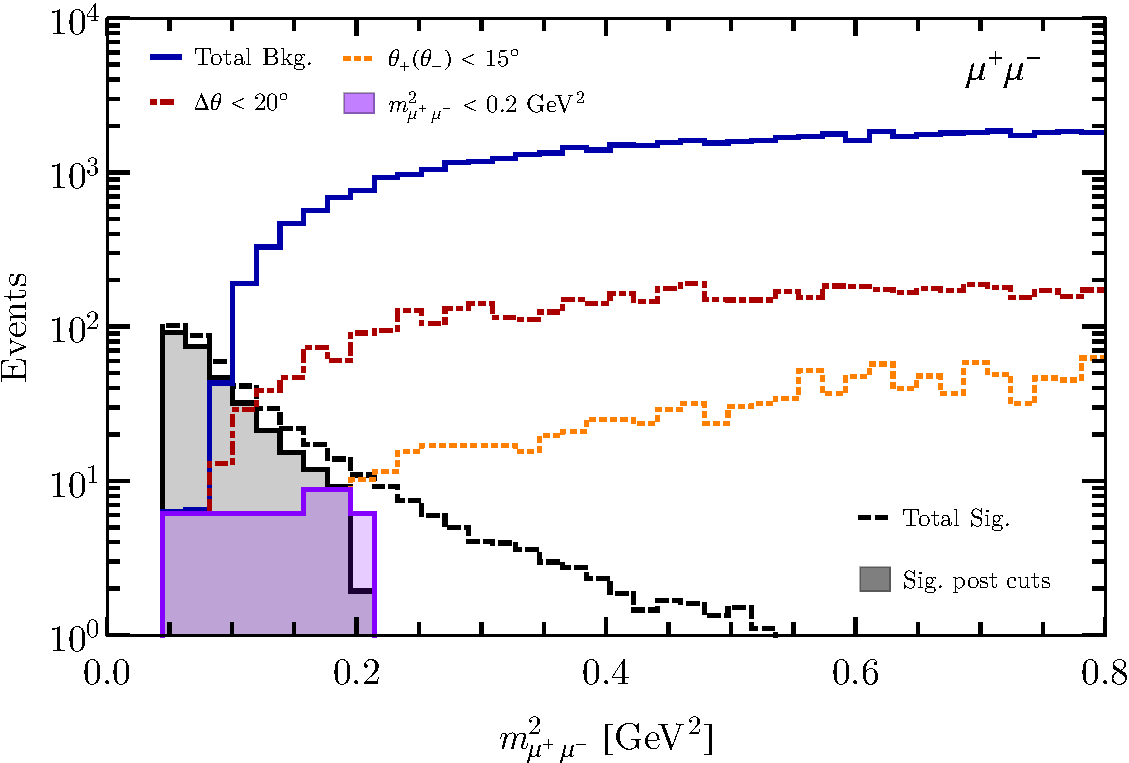
\includegraphics[width = 0.75\textwidth]{figs/SigvsBkg.pdf}
 \caption[Kinematical cuts on background samples for dimuon tridents.]{Signal and background distributions in invariant mass. The total background events (blue) include the misID rates in table \reftab{tab:misIDlist}. We apply consecutive cuts on the background, starting with cuts on the separation angle $\Delta \theta$ (red), both charged lepton angles to the beamline ($\theta_+$ and $\theta_-$) (orange) and the invariant mass $m^2_{\mu^+ \mu^-}$ . We show the signal samples before and after all the cuts in dashed black and filled black, respectively. \label{fig:bkg_flow}}
\end{figure}
%
Finally, we comment on some of the limitations of our analysis. The low rate of trident events calls for a more careful evaluation of other subdominant processes that could be easily be overlooked. For channels involving electrons, it is possible that de-excitation photons and internal bremsstrahlung become a source of background, as these also produce very soft EM showers, none of which are implemented in GENIE. The question of reconstruction of these soft EM showers, accompanied either by a high energy muon or by another soft EM shower also would have to be addressed, especially in the latter case where a trigger for these soft events would have to be in place. A more complete analysis is also needed for treating the decay products of charged pions and muons produced in neutrino interactions, as well as rare meson decay channels (like the Dalitz decay of neutral pions $\pi^0 \to \gamma e^+ e^-$). Cosmic ray events are not expected to be a problem due to the requirement of a vertex and a correlation with the beam for trident events. Perhaps even more exotic processes, such as the production of three final-state charged leptons ($\nu_{\alpha} (\overline{\nu}_{\alpha}) + \mathcal{H} \to  \ell_\alpha^- (\ell_\alpha^+) + \ell_\beta^+ + \ell_{\beta}^- + \mathcal{H^\prime}$), can also become relevant. For instance, radiative trimuon production \cite{Smith:1977nx} can potentially serve as a background to dimuon tridents if one of the muons is undetected. Similarly, $\mu e e$ production would fake a dielectron (mixed) trident signature if the muon (an electron) is missed. We are not aware of any estimates for the rate of these processes at the DUNE ND, but we note that their rate can be comparable to trident production at energies above $30$ GeV \cite{Albright:1978mg}. Improvements on our analysis should come from the collaboration's sophisticated simulations, allowing for a better quantification of hadronic activity, more realistic misID rates and more accurate detector responses.  

%%%%%%%%%%%%%%%%%%%%%%%%%%%%%%%%%%%%%%%%%%%%%%%%%%%%
\section{Conclusions}

\label{sec:conc}
Neutrino trident events are predicted by the SM, however, only $\overline{\nu}_\mu$ initiated dimuon tridents have been observed in small numbers, typically fewer than 100 events. This will change in the near future thanks to the current and future generations of precision neutrino scattering and oscillation experiments, which incorporate state-of-the-art detectors located at short distances from intense neutrino sources. 
%
In this work we discuss the calculation of the neutrino trident cross section for all flavours and hadronic targets, and provide estimates for the number and distributions of events at 9 current or future neutrino detectors: five detectors based on the new LAr technology (SBND, $\mu$BooNE, ICARUS, DUNE ND and $\nu$STORM ND) as well as four more conventional detectors (INGRID, MINOS ND, NO$\nu$A ND and MINER$\nu$A). The search for tridents, however, need not be exclusive to near detectors of accelerator neutrino experiments. As pointed out by the authors of Ref.~\cite{Ge2017}, atmospheric neutrino experiments can also look for these processes, benefiting from the increase of the cross section at large energies. 

We have stressed the need for a full four-body phase space calculation of the trident cross sections without using the EPA. This approximation has been employed in recent calculations and can lead to overestimations of the cross section by 200\% or more at the peak neutrino energies relevant for many accelerator neutrino experiments.
%
Moreover, we show why the EPA is not applicable for computing trident cross sections, and provide the first quantitative assessment of this breakdown for coherent and incoherent hadronic regimes. 
%
We find that the breakdown of the approximation is most severe for processes with electrons in the final-state and for incoherent scattering of all final state flavours. 
%
For coherent dimuon production, the approximation can give a reasonable result at large neutrino energies. This is due to the nuclear form factors that serendipitously suppress those regions of phase space where the EPA is least applicable. We also demonstrated that the best results in this channel are achieved when applying artificial cuts to the phase space.
%
However, even in this case, at energies relevant for the above experiments, the EPA can artificially suppress the coherent scattering contribution and increase the incoherent one giving rise to an incorrect rate and distributions of observable quantities. 
%
For instance, the invariant mass of the charged lepton pair $m^2_{\ell \ell}$ and their angular separation $\Delta \theta$ are more uniformly distributed for incoherent than for coherent trident scattering. Using the correct distributions is crucial to correctly disentangle the signal from the background by cutting on these powerful discriminators.

Our calculations show that DUNE ND is the future detector with the highest neutrino trident statistics, more than 6000 mixed events, 11\% produced by incoherent scattering, more than 1900 dielectron events, 5\%  produced by incoherent scattering and about 750 dimuon events,
almost 34\% of those produced by a incoherent process. Making use of our efficiencies (see \reftab{tab:DUNE_ND_NU_BG}), assuming an ideal background suppression and neglecting systematic uncertainties, we quote the statistical uncertainty on the coherent-like flux averaged cross section for the DUNE ND. We do this for coherent only events and, in brackets, for coherent plus incoherent events, yielding
%
\[\frac{\delta \langle \sigma^{e^\pm\mu^\mp} \rangle}{\langle \sigma^{e^\pm\mu^\mp} \rangle} =  1.8\% \, (1.6\%), \quad \frac{\delta \langle \sigma^{e^+e^-} \rangle}{\langle \sigma^{e^+e^-} \rangle} =  3.4\% \,(3.3\%) \quad \mathrm{and} \quad \frac{\delta \langle\sigma^{\mu^+\mu^-} \rangle}{\langle \sigma^{\mu^+\mu^-} \rangle} =  5.5\% \,(5.1\%).\]
%
In this optimistic framework we expect the true statistical uncertainty on coherent-like tridents to lie between the two numbers quoted, depending on how many incoherent events contribute to the coherent-like event sample. This impressive precision would provide unprecedented knowledge of the trident process and the nuclear effects governing the interplay between coherent and incoherent regimes. We emphasize, however, that given these small values for the relative uncertainties, the trident cross section will likely be dominated by systematic uncertainties from detector response and backgrounds which are not modelled here. 

For DUNE ND, we have studied the distribution of observables which could help distinguish trident events from the background. We have estimated the background for each trident channel via a Monte Carlo simulation using GENIE, and identified the dominant contributions arising primarily from particle misidentification.  
%
We conclude that reaching background rates of the order 
${\cal O}(10^{-6}-10^{-5})$ times the CC rate is necessary to observe trident events at DUNE ND, and given the distinctive kinematic behaviour of the trident signal a simple cut-based GENIE-level analysis suggests that this is an attainable goal in a LAr TPC. 

Existing facilities may also be able to make a neutrino trident measurement at their near detectors. Despite not including reconstruction efficiencies nor an indication of the impact of backgrounds, we find that the largest trident statistics is available at INGRID, the T2K on-axis near detector. We predict about 660 (1700) events for the mixed flavour, 300 (770) events for the dielectron and 50 (130) events for the dimuon channel for T2K-I (T2K-II). The more fine-grained near detector of MINOS and MINOS+ is also expected to have collected a significant numbers of events during its run. As such, the very first measurement of neutrino trident production of mixed and dielectron channels may be at hand.


%%%%%%%%%%%%%%%%%%%%%%%%%%%%%%%%
\section{Individual Backgrounds}
\label{app:backgrounds}
Here we discuss backgrounds to trident final-states in more detail. We start by motivating our misID rates shown in \reftab{tab:misIDlist}, and then discuss the dominant background processes individually.

In LAr photons can be distinguished from a single electron if their showers start displaced from the vertex (if present). Photons have a conversion length in LAr of around 18 cm, meaning $5$--$10\%$ could be expected to convert quickly enough to hinder electron-photon discrimination by this means if the resolution on the gap is from $1$--$2$ cm \cite{Acciarri:2016sli}. Once pair conversion happens, photons can be distinguished from a single electron purely by $\dd E/\dd x$ measurements in the first 1--2 cm of their showers. Motivated by the success of this method as shown at ArgoNeuT \cite{Acciarri:2016sli} and based on projections for DUNE \cite{Acciarri:2016ooe}, we assume that $5\%$ of photons would be taken as $e^\pm$ with perfect efficiency, without the need for an event vertex. Needless to say that a dedicated study for trident topologies would be necessary for a more complete study. It is worth noting that our remarks concern only the misID of a single photon for a single electron, whilst the distinction between a photon and an overlapping $e^+e^-$ pair without a vertex can be much more challenging. For this reason we take the misID rate between an overlapping $e^+e^-$ pair and a photon to be 1 in the absence of a vertex.  

Charged pions are notorious for faking long muon tracks. We estimate this misID rate as arising from through-going pions, which do not exhibit the decay kink used in their identification. We assume an interaction length of around $1$ m, meaning that about $5\%$ of particles travel $\sim3$ meters and escape the fiducial volume. Assuming that this is the most likely way a pion can spoof a muon, we estimate a naive suppression rate of $10^{-2}$. In a more complete study, it is desirable to explore the length of the muon and pion tracks inside the detector as a function of energy. The length of the contained tracks can also be an important tool for background suppression which we leave to future studies.  

%%%%%%%%%%%%%%%%%%%%%%%%%%%%%%%%%%%%%%%%%%%%%%%%%%%%
\subsection{Pion Production}

Coherent pion production in its charged ($\nu + A \to \ell^\mp + \pi^\pm + A$) and neutral ($\nu + A \to \nu + \pi^0 + A$) current version is very abundant at GeV energies. The cross section for these processes is modelled in GENIE using a modern version of the Rein-Sehgal model \cite{REIN198329,Rein:2006di}. The charged current version serves mainly as a background to $\mu^+ \mu^-$ tridents, but can also appear as a background for $e^\pm \mu^\mp$ tridents for incoming electron neutrinos or antineutrinos. It has been studied before at MiniBooNE \cite{AguilarArevalo:2010xt}, MINER$\nu$A \cite{Higuera:2014azj,Mislivec:2017qfz}, T2K \cite{Abe:2016fic,Abe:2016aoo}, and for the first time in LAr at ArgoNeuT \cite{Acciarri:2014eit}. This process has a very distict low 4-momentum transfer to the nucleus $|t|$ \cite{Higuera:2014azj}, but a much flatter distribution in invariant mass if compared to trident. The neutral current version of coherent pion production serves as a background to $e^+e^-$ tridents. This process has been studied before by the MiniBooNE \cite{AguilarArevalo:2009ww}, SciBooNE \cite{Kurimoto:2010rc} and in LAr by the ArgoNeuT collaboration \cite{Acciarri:2015ncl}. There are two possibilities for these events to fake an $e^+e^-$ trident: when one of the gammas produced in the $\pi^0$ decay is missed and the other is misIDed for an overlapping $e^+e^-$ pair, and when both photons are each misIDed for a single electron. This signature also comes with low hadronic activity, but for separated visible photons the invariant mass is a natural discriminator, as in the detector $m_{\gamma \gamma} \approx m_{\pi^0}$.

Resonant pion production can also contribute to trident backgrounds in the absence of any reconstructed protons. Resonant pion production can be larger than its coherent counterpart and is modelled in GENIE by the Rein-Sehgal model \cite{Rein:1980wg}. Its CC version was measured by MiniBooNE \cite{AguilarArevalo:2010xt}, K2K \cite{Mariani:2010ez}, MINOS \cite{Adamson:2014pgc}, and MINER$\nu$A \cite{Altinok:2017xua}. In the latter measurement one can clearly see the large number of events with undetected protons. The misIDed photon and the charged lepton invariant mass are once more flatter than the trident ones, allowing for a kinematical discrimination whenever a single photon is undetected. It is worth noting that these are some of the dominant underlying processes for pion production in GENIE, but all events leading to topologies relevant for trident are included in our analysis.
%
%%%%%%%%%%%%%%%%%%%%%%%%%%%%%%%%%%%%%%%%%%%%%%%%%%%%
\subsection{Charm Production}

Since the first observation of dimuon pairs from charm production in neutrino interaction by the HPWF experiment in 1974 \cite{Benvenuti:1975ru}, a lot has been learned about these processes (see \cite{Lellis:2004yn} for a review) in neutrino experiments. Particularly, the production of charm quarks and their subsequent weak decays into muons or electrons have been identified as a major source of background for early trident searches. At the lower neutrino energies at DUNE, however, this is expected to be a smaller yet non-negligible contribution. From our GENIE samples, we estimate that a charmed state is produced at a rate of around $10^{-4}(N_\text{CC}+N_\text{NC})$. Most of these produce either D mesons, 
$\Lambda_c$ or $\Sigma_c$ baryons. These particles decay in chains, emitting a muon with a branching ratio of around $0.1$, and are always accompanied by pions or other hadronic particles. We therefore expect these rates to be negligible with a hadronic veto, and do not consider them further. We hope, however, that future studies will address these channels in more detail.

%%%%%%%%%%%%%%%%%%%%%%%%%%%%%%%%%%%%%%%%%%%%%%%%%%%%
\subsection{CC$\gamma$ and NC$\gamma$}

The emission of a single photon alongside a CC process could be a background for $\mu e$ tridents if the photon is misIDed as a single electron. When the photon is produced in a NC event, it can be a background to overlapping $e^+e^-$ tridents. In GENIE, these topologies arise mainly due to resonance radiative decays and from the intra-nuclear processes. For this reason, it usually comes accompanied with extra hadronic activity. For hadronic resonances, we have simulated CC processes in GENIE and estimated
the multiplicities: $0.5\%$ single
photon and $1\%$ double photon emission from CC rates. Radiative photon production from the charged lepton, on the other hand, does not need to come accompanied by hadrons. It is phase space and $\alpha\approx1/137$ suppressed with respect to CCQE rates, and therefore could occur at appreciable rates compared to our signal. This contribution, however, is not included in GENIE and is absent from our samples. The rates of internal photon bremsstrahlung have been estimated before, particularly for T2K where a low-energy photon is an important background for electron
appearance searches \cite{Efrosinin:2009zz}, and as a background to the low energy events at MiniBooNE \cite{Bodek:2007wb}. De-excitation gammas from the struck nuclei can also generate CC$\gamma$ or NC$\gamma$ topologies \cite{PhysRevLett.108.052505}. These contributions for Ar are not included in GENIE, but are expected to come with a distinct energy profile, which can be tagged on.

%%%%%%%%%%%%%%%%%%%%%%%%%%%%%%%%%%%%%%%%%%%%


\chapter{Conclusions}
Particle physics is at a very important moment of its history. The Standard Model (SM) provides unprecedented accuracy when describing particle physics data, but it provides no explanation for neutrino masses and the existence of dark matter (DM). It is tempting to think that these phenomena are to the Standard Model what blackbody radiation was to classical physics in the beginning of the 20th century, a scientific revolution on the wait. While we cannot be sure, we continue to devise new theoretical explanations and new methods to test them. In particular, the experimental efforts in neutrino physics open new possibilities to test the connections between neutrinos and beyond the SM physics. New detector technologies, such as liquid Argon (LAr), and more powerful neutrino beams, allow us to study neutrino interactions in great detail and mimic conditions of high intensity fixed-target and beam-dump facilities. 

Rare and well-understood neutrino scattering processes offer a unique tool to test the SM weak interactions. We have shown that measuring the neutrino trident production ($\nu \, A \, \to \, \nu \, \ell \, \ell \, A$) cross section at GeV energies will be an attainable goal of near future experiments such as the Deep Underground Neutrino Experiment (DUNE). The backgrounds in LAr are expected to be manageable within our assumptions for particle identification capabilities. Our calculation for the cross section makes it explicit the poor performance of the Equivalent Photon Approximation for this process, and provides an estimate for trident rates at various current and future neutrino facilities. In Chapter 4, we assess the sensitivity of DUNE to new anomaly-free leptophilic $U(1)_{L_\alpha - L_\beta}$ groups. The new $Z^\prime$ gauge bosons can be searched for in leptonic and semi-leptonic neutrino scattering processes, such as neutrino trident and neutrino-electron scattering ($\nu \, e \to \nu \, e$). We showed that for $L_e - L_\mu$, the new boson may be searched for in neutrino-electron scattering measurements, provided the neutrino flux uncertainties are kept under control. For $L_\mu - L_\tau$, neutrino trident production of dimuon pairs can set strong bounds on the coupling and masses of the $Z^\prime$ boson, otherwise much harder to constrain since it does not couple to the first SM generation of particles. We show that if the number of non-trident background events exceeds that of the number of SM tridents, then DUNE starts to lose its ability to probe the entire parameter space able to explain the muon $(g-2)_\mu$. 

A new set of models for low energy phenomenology in neutrino experiments has been developed in Chapter 5. The model contains a new dark neutrino state $\nu_D$, charged under a hidden $U(1)^\prime$ local gauge symmetry, which in turn is broken by the vev of a new scalar $\Phi$. The setup realises all three neutral and renormalizable portals to hidden sectors: the scalar, vector and neutrino portals. With the presence of a completely neutral state $N$, this closely resembles other low-scale seesaw models like the inverse and extended seesaw. We show how the phenomenology is very different from having each portal taken individually, opening up parameter space to explain experimental anomalies such as the muon $(g-2)$, and the MiniBooNE low energy anomaly. As it turns out, the model also radiatively generates light neutrino masses, while remaining testable at the MeV scale.  

Phenomenological realizations of the dark neutrino model had already been put forward as explanations of the excess of electron-like events at MiniBooNE. As shown in Chapter 6, light $Z^\prime$ scenarios are severely constrained by neutrino-electron scattering measurements at accelerator neutrino experiments. We proposed a new technique to constrain these models by investigating sideband data in the MINER$\nu$A low energy measurement, as well as in the past measurements performed by CHARM-II. By using simplified rate analysis in sideband regions of MINER$\nu$A and CHARM-II, as well as computing the MiniBooNE angular spectrum, we showed that the region where both energy and angular distributions at MiniBooNE can be explained in this model are in severe tension with neutrino-electron scattering data. Although not all parameter space is excluded, our work highlights the importance of the coherent photon-like sidebands in neutrino-electron scattering measurements and paves the way for future analyses at MINER$\nu$A, NO$\nu$A, and DUNE, eventually.

Neutrino beams from stored muons can bring great improvements to laboratory neutrino experiments. The \nus project is a first step towards neutrino factories and muon colliders, and may provide a definite test of whether short-baseline oscillations due to eV sterile neutrinos exist. Beyond testing existing anomalies, it could provide the most stringent limits on non-unitarity of the PMNS matrix due to light sterile neutrinos. Our analysis also highlighted the peculiarities of the beam, with implications for production localisation, short-baseline CP violation, and displaying a variety of oscillation channels in a single experiment.

Neutrino physics is a field full of exciting and unexpected results. Neutrino oscillations have marked the beginning of our exploration of beyond the SM physics, but much more is yet to be learned. Beyond studying the physics of neutrino flavour, neutrino oscillation and scattering experiments are a unique tool to probe the weak interactions and to search for new particles. The theoretical models, novel measurements, and analyses techniques we have proposed in this thesis are intimately connected to the unique properties of neutrinos. Whether neutrinos are indeed a gateway to dark sectors, or just what we need to rule this possibility out, we are confident that the bright future of neutrino physics will shine light on what lies beyond the SM.

\appendixpageoff
\begin{appendices}
\let\clearpage\relax
\chapter{Phase Space}
In this appendix we derive some key results for the phase space treatment we use in calculating cross sections and decay rates. We begin with the factorization of $N$-final state phase-space factors into $N-2$ two-body ones. In general, the $N$-body phase space can be written as 

\begin{equation}
 \dd \Phi_{N} (P,\{p_i\}) = (2 \pi)^4 \delta^4 (P - \sum_i^N p_i) \, \prod_i^{N}\, \frac{\dd^3 p_i}{(2\pi)^3 2 E_i},
\end{equation}
where $\{p_i\} = p_1, \ldots, p_N$. Focusing on the 1-2 subsystem with total momentum $p_{12} = p_1 + p_2$, we can write

\begin{align}
  \dd \Phi_{N} (P,\{p_i\}) =& \int \dd^4 p_{12} \, \delta^4 (p_{12} - p_1 - p_2) \, (2 \pi)^4 \delta^4 (P - \sum_i^N p_i) \, \prod_i^{N}\, \frac{\dd^3 p_i}{(2\pi)^3 2 E_i}  \nonumber\\
 =& \int \dd^4 p_{12}\, \dd \Phi_2 (p_{12}, p_1, p_2) \, (2 \pi)^4 \delta^4 (P - p_{12} - \sum_{i=3}^N p_i) \, \prod_{i=3}^{N}\, \frac{\dd^3 p_i}{(2\pi)^3 2 E_i}\nonumber\\
 =& \int \dd^4 p_{12} \, \dd m_{12}^2 \, \delta(p_{12}^2 - m_{12}^2) \, \dd \Phi_2 (p_{12}, p_1, p_2)\nonumber\\ &\hspace{20ex} \times  (2 \pi)^4 \delta^4 (P - p_{12} - \sum_{i=3}^N p_i) \, \prod_{i=3}^{N}\, \frac{\dd^3 p_i}{(2\pi)^3 2 E_i},
\end{align}
which from 

\[\int \dd^4 p_{12} \, \delta(p_{12}^2 - m_{12}^2) = \int \dd^4 p_{12} \, \frac{\delta (E_{12} - \sqrt{m_{12}^2 + |\vec{p}_{12}|^2})}{2\sqrt{m_{12}^2 + |\vec{p}_{12}|^2} } = \int \frac{\dd^3 p_{12}}{2 E_{12}}, \]
yields the final results
\begin{equation}
 \dd \Phi_{N} (P, p_1, \ldots, p_N) = \frac{\dd m_{12}^2}{2 \pi} \dd \Phi_2 (p_{12}, p_1, p_2) \dd \Phi_N (P, p_{12}, p_3,\ldots,p_N). 
\end{equation}

This result not only lets us factorize any resonant features in phase space, but also provides a recipe to tackle the kinematics of any process in terms of a series of 2-body problems, which are much simpler. The 2-body phase-space factors and associated four-momenta in the respective center-of-mass (CM) frame can always be written as

\begin{align}
\dd \Phi_2 (p_{12}, p_1, p_2) &= \frac{{\lambda^{1/2} \left( 1, m_1^2/E_{12}^{ {\rm CM} \, 2}, m_2^2/E_{12}^{ {\rm CM} \, 2} \right)} }{32 \pi^2 } \dd \Omega^{\rm CM},\nonumber\\
p_{12} &= \left(E_{12}^{ {\rm CM}}, \vec{0} \right),\nonumber\\
p_{1}  &= \left(\frac{E_{12}^{ {\rm CM} \, 2}+m_1^2-m_{2}^2}{2E_{12}^{ {\rm CM} \, 2}}, |\vec{p}_1| \sin{\theta} \cos{\phi}, |\vec{p}_1| \sin{\theta} \sin{\phi} , |\vec{p}_1| \cos{\theta} \right),\nonumber\\
p_{2}  &= \left(\frac{E_{12}^{ {\rm CM} \, 2}+m_{2}^2 - m_1^2}{2E_{12}^{ {\rm CM} \, 2}}, -\vec{p}_1 \right),
\end{align}
where $\lambda(a,b,c) = (a - b -c)^2 - 4 b c$ is the K\"all\'en function. Now, the problem is reduced to finding the CM frame of every $p_{ij}$ subsystem, and the transformation between all such frames, if necessary. Of course, the dependence of the matrix element on the kinematics makes certain phase space parametrization better than others, making each problem unique. Lab variables, for instance, are the standard parametrization for DIS scattering as they preserve crucial physical intuition of the process at hand.

\paragraph{Neutrino trident production} Now we derive a phase space parametrization for neutrino trident production in terms of the momentum transfer $K^2 =  2 p_1 \vdot p_2$. This is important if one wants to change variables to smooth out the integrand at low $M_{Z^\prime}$ masses. We follow the calculation in \cite{Czyz1964} and \cite{Ballett:2018uuc}, and proceed to define $K^2$ as one of the integration variables. The relevant Lorentz invariant phase space for the $2\to3$ leptonic part of the cross section is given by
%
\begin{align}
\int \dd^3 & \Pi_{\mathrm{LIPS}} = \nonumber\int \frac{\dd \vec{p_2} }{(2\pi)^32 E_2} \frac{ \dd \vec{p_3} } {(2\pi)^3 2 E_3} \frac{\dd \vec{p_4}}{(2\pi)^32 E_4} \\& (2\pi)^4\delta^{(4)} (p_1 + q - p_2 - p_3 - p_4).
\end{align}
%
Following \cite{Czyz1964} we start by working in the frame $\vec{p_1} + \vec{q} - \vec{p_3} = 0$, putting $\vec{p_1}$ along the $\hat{z}$ direction instead. The delta function can be integrated with the $\vec{p_4}$ and $|\vec{p_2}|$ integrals, such that 
%
\begin{equation}
 \int \frac{\dd \vec{p_2} }{2 E_2} \frac{\dd \vec{p_4}}{2 E_4} \, \delta^{(4)} (p_1 + q - p_2 - p_3 - p_4) =  \int \frac{ |\vec{p_2}|}{4 W_c} \, \frac{1}{E_1 E_2} \dd K^2 \, \dd \phi_2,
\end{equation}
%
where we defined
%
\begin{align}
&|\vec{p_2}| = (W_c^2 - m_1^2)/2W_c, \nonumber\\\nonumber &W_c = q^0 + E_1 - E_3, \\ &K^2 = 2 E_1 E_2 (1 - \cos{\theta_2}).
\end{align}
%
Since we conserve energy and momentum in this frame, we can take $-1 \leq \cos{\theta_2} \leq 1$ and $0 \leq \phi_2 \leq 2 \pi$. The remaining $\vec{p_3}$ integral can be performed with the variables defined in \cite{Czyz1964} to yield
%
\begin{equation}
 \int \frac{\dd \vec{p_3} }{2 E_3}  =  \int \frac{2 \pi}{\hat{s}} \, \dd x_5 \, \dd x_3,
\end{equation}
%
where a trivial azimuthal angle was integrated over. Their limits are more easily found in the frame $\vec{p_1} + \vec{q} = 0$, with $\vec{q}$ along the $\hat{z}$ direction. Finally, our main result is given by
%
\begin{equation}
\int \dd^3 \Pi_{\mathrm{LIPS}} = \frac{1}{(2\pi)^4} \int \frac{|\vec{p_2}|}{4 W_c} \, \frac{1}{\hat{s}} \, \frac{1}{E_1 E_2} \, \dd x_5 \, \dd x_3 \, \dd K^2 \, \dd \phi_2 .
\end{equation}
%
There remains two non-trivial integrations to be performed to obtain the full 4-body phase space cross section, namely the ones over $q^2$ and $\hat{s}$. The substitutions suggested in \cite{Lovseth1971} for these two invariants are still convenient, and we make use of them in our numerical integrations.


\cleardoublepage
\chapter{One loop $\nu$ masses in Type-I seesaw}
\section{Type-I seesaw neutrino masses in the SM}

In this appendix, we compute the one-loop corrections to the light neutrino masses in the SM, following Refs.~\cite{Kniehl:1996bd,Grimus:2002nk,AristizabalSierra:2011mn}.

We work with the on-shell (OS) renormalization scheme. This is ensured by requiring that the off-diagonal elements of the self-energy be diagonal when the external particles are on their mass shell, and that the residue of the renormalized propagator are equal to one. Note this is only applicable to the off-diagonal entries that involve at least one heavy neutrino, and that the light-light entries are all non-zero and finite at one-loop.

Assuming Majorana neutrino fields, one can write the self-energy tensor in its most general form:
%
\begin{equation}
  \Sigma_{ij} (\slashed{q}) = \slashed{q} {\rm P}_L \Sigma_{ij}^L (q^2) + \slashed{q} {\rm P}_R \Sigma_{ij}^R (q^2) +  {\rm P}_L \Sigma_{ij}^M (q^2) +  {\rm P}_R \Sigma_{ij}^{M*} (q^2),
\end{equation}
%
where by virtue of the Majorana nature the previous terms obey
\[\Sigma_{ij}^L (q^2) = \Sigma_{ij}^{R*} (q^2), \qquad \Sigma_{ij}^M (q^2) = \Sigma_{ji}^M (q^2). \]

\subsection{Self-energy}

We now compute explicitly the self-energy corrections. The contribution from the scalar fields $s= h^0, \varphi^0$, the goldstones $G = G_h, G_\varphi$ and the vector bosons $V = Z, Z^\prime$ are 

\begin{align*}
 -i\,\Sigma^s_{ij} (p^2) &= (-i)^2 \left(\Delta_s P_R + \Delta^*_s P_L \right)_{ik} \times\\&\qquad\qquad \int \frac{d^d k}{(2\pi)^d} \frac{i (\slashed{p} + \slashed{k} + m_k) }{(p+k)^2 - m_k^2} \frac{i}{k^2 - m_s^2} \left( \Delta_s P_R + \Delta^*_s P_L \right)_{kj},\\
 %
 -i\,\Sigma^G_{ij} (p^2) &= (-i)^2 \left(i\,\Delta_G P_R + i\,\Delta^*_G P_L \right)_{ik} \times\\&\qquad\qquad\int \frac{d^d k}{(2\pi)^d} \frac{i (\slashed{p} + \slashed{k} + m_k) }{(p+k)^2 - m_k^2} \frac{i}{k^2 - \xi_V m_V^2} \left( i\,\Delta_G P_R + i\,\Delta^*_G P_L  \right)_{kj},\\
%
 -i\,\Sigma^G_{ij} (p^2) &= -(-i)^2 \gamma^\mu \left( C_V P_L - C_V^T P_R \right)_{ik} \times \\&\qquad\qquad\int \frac{d^d k}{(2\pi)^d} \frac{i (\slashed{p} + \slashed{k} + m_k) }{(p+k)^2 - m_k^2} \frac{iP_{\mu\nu}}{k^2 - m_V^2} \gamma^\nu \left( C P_L - C^T P_R \right)_{kj},
\end{align*}
with no index summation notation. In the latter term, we defined the vector boson propagator numerator, which we rewrite as
%
\begin{align*}
\gamma^\mu P_{\mu\nu} \gamma^\nu &= \gamma^\mu \left[ g_{\mu\nu} - (1-\xi_V) \frac{k_\mu k_\nu}{k^2 - \xi_V m_V^2} \right] \gamma^\nu\\
&= d - (1-\xi_V) \frac{k^2 - m_k^2}{k^2 - \xi_V m_V^2} - \frac{m_k^2}{m_V^2} \frac{ (k^2 - \xi_V m_V^2) - (k^2 - m_V^2)}{k^2 - \xi_V m_V^2}.
\end{align*}

This allows us to write the relevant part of the self-energy as functions of the scalar two-point loop function
\begin{align}
 B_0 (l, m_a^2,m_c^2) = \mu^{2\epsilon} \int \frac{d^d k}{(2 \pi)^d} \frac{1}{(k^2-m_a^2)( (l+k)^2 - m_c^2 )},
\end{align}
such that
\begin{align}
  \Sigma^s_{ij} (0) \, P_R =& -\frac{\pi^2}{(2\pi)^4} \mu^{d-4} \left[ (\Delta_s)_{ik} m_k B_0 (0,m_k^2, m_s^2) (\Delta_s)_{kj}\right] \, P_R \\
%
 \Sigma^G_{ij} (0) \, P_R =& \frac{\pi^2}{(2\pi)^4} \mu^{d-4} \left[ (\Delta_G)_{ik} m_k B_0 (0,m_k^2, \xi_V m_V^2) (\Delta_G)_{kj}\right] \, P_R \\
%
 \Sigma^V_{ij} (0) \, P_R =& -\frac{\pi^2}{(2 \pi)^4} \mu^{d-4} \left[ (C_V)_{ik} m_k \,f( m_k^2, m_V^2, \xi m_V^2) (C_V^*)_{kj} \right] \, P_R,
\end{align}
where the rearrangement of the boson propagator allowed us to write $f( m_k^2, m_V^2, \xi m_V^2)$ as
\begin{align*}
f( m_k^2, m_V^2, \xi m_V^2) =&\, d\, B_0(0,m_k^2, m_V^2) - (1-\xi_V) B_0 (0,m_V^2, \xi_V m_V^2) +\\ & \frac{m_k^2}{m_V^2} B_0 (0, m_k^2, \xi_V m_V^2) - \frac{m_k^2}{m_V^2} B_0 (0,  m_k^2, m_V^2). 
\end{align*}

Finally, the scalar loop function is given by
\begin{align*}
 B_0 (0,m_a^2,m_b^2) &= \frac{1}{\epsilon} - \gamma_E + \ln{4 \pi} - \int_0^1 dx \ln{\frac{m_a^2-x(m_a^2 - m_b^2)}{\mu^2}}\\
 &= \frac{1}{\epsilon} - \gamma_E + \ln{4 \pi} - \frac{m_a^2}{m_b^2 - m_a^2} \left[ \ln{\frac{m_a^2}{\mu^2}}  - 1 \right] + \frac{m_b^2}{m_b^2 - m_a^2} \left[ \ln{\frac{m_b^2}{\mu^2}}  - 1 \right].
\end{align*}

The finiteness of our final result and its gauge invariance are a consequence of the two following identities
\begin{align}
 \Delta_G = \Delta_S = C \frac{\hat{m}}{m_V} + \frac{\hat{m}}{m_V}C^T, \quad \quad C \hat{m} C^T = 0.
\end{align}

For light neutrinos ($i,j=1,2,3$), the final result reads

\begin{align}
 \Sigma_{ij} P_R  = -\frac{\pi^2}{(2\pi)^4} C \hat{m}\left[ d\, B_0(0,\hat{m}^2,m_V^2) + \frac{\hat{m}^2}{m_V^2} \left( B_0 (0,\hat{m}^2,m_S^2) - B_0(0,\hat{m}^2,m_V^2) \right) \right] C^T P_R.
\end{align}

\end{appendices}

\bibliographystyle{JHEP}
\bibliography{introduction/introduction,theory/theory,tridentSM/tridentSM,Zprime_scattering/Zprime_scattering,miniboone/miniboone,appendices/loop_masses}

\end{document}
